\documentclass[a4paper]{report}

%Import thesis style file
\usepackage{baththesis}
%Define thesis style macros and names
\title{Asymptotic and Numerical Analysis of Wave Propagation in Thin-Structure Waveguides}
\author{William Michael Graham}
\degree{Doctor of Philosophy}
\department{Department of Mathematical Sciences}
\degreemonthyear{June 2022}

%Image and page layout packages
\usepackage{graphicx}
\usepackage{subcaption} %allows subfigures
\usepackage[bottom]{footmisc} %footnotes go below figures
\usepackage{parskip} %adds line space between paragraphs by default
%Declare location of image files
\usepackage{appendix} %can declare chapter-local appendices

\DeclareGraphicsRule{.tif}{png}{.png}{`convert #1 `dirname #1`/`basename #1 .tif`.png}
\graphicspath{{./Diagrams/Diagram_PDFs/} {./Diagrams/Numerical_Results/}}

%Allows for more options when enumerating lists (roman, lettering, etc)
\usepackage{enumerate}

%\input imports all commands from the target files
%The idea behind this file is that it will be used to store all the maths-related macros that I concoct; so that I can import all the commands by \input{this file} in the preamble of any file that I want to use them in.
%This should make the top-level files look a lot cleaner, and the preamble much shorter!

\usepackage{amssymb}
\usepackage{amsmath}
%\usepackage{mathtools}

%theorems and lemma etc setup using amsthm
\usepackage{amsthm}
\theoremstyle{definition}
\newtheorem{definition}{Definition}[section]
\theoremstyle{plain}
\newtheorem{theorem}{Theorem}[section]
\theoremstyle{plain}
\newtheorem{lemma}[theorem]{Lemma}
\theoremstyle{plain}
\newtheorem{prop}[theorem]{Proposition}
\theoremstyle{plain}
\newtheorem{cory}[theorem]{Corollary}
\theoremstyle{definition}
\newtheorem{convention}[theorem]{Convention}
\theoremstyle{definition}
\newtheorem{assumption}[theorem]{Assumption}
\theoremstyle{definition}
\newtheorem{conjecture}[theorem]{Conjecture}

\allowdisplaybreaks %allows equations in the same align environment to split over multiple pages.

%tstk always need be there
\newcommand{\tstk}[1]{\textbf{#1} \newline}

%this adds extra functionality to pmatrix, vmatrix, bmatrix etc by allowing you to pass an optional argument in [FACTOR] to multiply the default spacing between elements by FACTOR
\makeatletter
\renewcommand*\env@matrix[1][\arraystretch]{%
  \edef\arraystretch{#1}%
  \hskip -\arraycolsep
  \let\@ifnextchar\new@ifnextchar
  \array{*\c@MaxMatrixCols c}
  }
\makeatother

%begin the macros via newcommand. Try to group them up reasonably!

%notation and variable use throughout the file
\renewcommand{\vec}[1]{\mathbf{#1}}				%vectors are bold, not overline arrow
\newcommand{\recip}[1]{\frac{1}{#1}}			%fast reciprocal as a fraction
\newcommand{\interval}[1]{\sqbracs{0,\abs{#1}}}	%creates the closed interval from 0 to the length of the input #1, denoted by absolute value
\newcommand{\eps}{\varepsilon}					%pretty epsilons
\newcommand{\charFunc}[1]{\mathcal{I}_{#1}}%{\mathbb{1}_{#1}}		%characteristic function of a set
\newcommand{\sgn}{\mathrm{sgn}}

\newcommand{\dddom}{\widetilde{\Omega}}		%3D domain notation
\newcommand{\ddom}{\Omega}						%2D domain notation
\newcommand{\dddmes}{\widetilde{\mu}}			%2D sing. measure + point masses
\newcommand{\ddmes}{\mu}						%2D sing. measure
\newcommand{\compMes}{\tilde{\lambda}}			%2D composite (Leb + sing) measure

\newcommand{\graph}{\mathbb{G}}					%graph variable
\newcommand{\vertSet}{\mathcal{V}}					%set of vertices rather than big V
\newcommand{\edgeSet}{\mathcal{E}}					%set of edges rather than large E, \graph = (V,E)
\newcommand{\wavenumber}{\kappa}				%fourier variable or wavenumber, not to confuse with jk subscripts!
\newcommand{\qm}{\theta}						%quasi-momentum parameter
\newcommand{\kt}{\bracs{\wavenumber, \qm}}		%(k, theta) pair
\newcommand{\dmap}{\Gamma_0}					%Dirichlet map
\newcommand{\nmap}{\Gamma_1}					%Neumann map
\newcommand{\dgmap}{\dmap^{\graph}}			%Dirichlet and Neumann maps with graph script for distinction
\newcommand{\ngmap}{\nmap^{\graph}}
\newcommand{\ag}{\mathcal{A}_\graph}			%caligraphic A with graph script for distinction
\newcommand{\effFreq}{\Lambda}					%Effective frequency sqrt(w^2-\wavenumber^2)
\newcommand{\conLeft}{\stackrel{\rightarrow}{\smash{\sim}\rule{0pt}{0.4ex}}} %j connects to k, j left
\newcommand{\conRight}{\stackrel{\leftarrow}{\smash{\sim}\rule{0pt}{0.4ex}}} %j connects to k, j right
\newcommand{\con}{\sim}							%j connects to k, indifferent of direction

%standard sets
\newcommand{\naturals}{\mathbb{N}}			%natural numbers
\newcommand{\integers}{\mathbb{Z}}			%integers
\newcommand{\rationals}{\mathbb{Q}}			%rational numbers
\newcommand{\reals}{\mathbb{R}}				%real numbers
\newcommand{\complex}{\mathbb{C}}			%complex numbers

%other notations
\newcommand{\rmi}{\mathrm{i}}				%imaginary unit i (RoMan font i)
\newcommand{\e}{\mathrm{e}}					%Euler number, e (Roman font e)

%brackets and norms
\newcommand{\bracs}[1]{\left( #1 \right)}				%encloses input in brackets
\newcommand{\sqbracs}[1]{\left[ #1 \right]}				%encloses input in square brackets
\newcommand{\clbracs}[1]{\left\{ #1 \right\}}			%encloses input in curly bracers
\newcommand{\abs}[1]{\left\lvert #1 \right\rvert}					%absolute value
\newcommand{\norm}[1]{\lvert\lvert #1 \rvert\rvert}		%norm 
\newcommand{\setVert}{\ \middle\vert \ }					%vertical bar for the middle of sets
\newcommand{\ip}[2]{\left\langle #1 , #2 \right\rangle}	%inner product

%function sets
\newcommand{\smooth}[1]{C^{\infty}\bracs{#1}}							%smooth functions
\newcommand{\ltwo}[2]{L^{2}\bracs{#1,\mathrm{d}#2}}						%general L^2 space
\newcommand{\gradSob}[2]{H^1_\mathrm{grad}\bracs{#1, \mathrm{d}#2}}		%gradient Sobolev space
\newcommand{\gradSobQM}[2]{H^1_{\qm, \mathrm{grad}}\bracs{#1, \mathrm{d}#2}} %gradient + i\qm Sobolev space
\newcommand{\tgradSob}[2]{H^1_{\qm, \mathrm{grad}}\bracs{#1, \mathrm{d}#2}} %coz words and standardisation
\newcommand{\ktgradSob}[2]{H^1_{\wavenumber,\qm,\mathrm{grad}}\bracs{#1, \mathrm{d}#2}}	%k,\qm-gradient Sobolev space
\newcommand{\curlSob}[2]{H^1_\mathrm{curl}\bracs{#1, \mathrm{d}#2}}		%curl Sobolev space
\newcommand{\tcurlSob}[2]{H^1_{\qm, \mathrm{curl}}\bracs{#1, \mathrm{d}#2}}		%curl + i\qm Sobolev space
\newcommand{\kcurlSob}[2]{H^1_{\wavenumber,\mathrm{curl}}\bracs{#1, \mathrm{d}#2}}	%k-curl Sobolev space
\newcommand{\ktcurlSob}[2]{H^1_{\wavenumber,\qm,\mathrm{curl}}\bracs{#1, \mathrm{d}#2}}	%k,\qm-curl Sobolev space
\newcommand{\ktcurlSobDivFree}[2]{\mathcal{H}^{\kt}\bracs{#1, \mathrm{d}#2}}					%k,\qm-curl, divergence-free Sobolev space
\newcommand{\supp}{\mathrm{supp}}										%support of a function
\newcommand{\dom}{\mathrm{dom}}								%domain of function (or operator i guess)

%grad and curl sets
\newcommand{\gradZero}[2]{\mathcal{G}_{ #1, \mathrm{d}#2}\bracs{0}}		%gradients of zero for domain #1 with measure #2
\newcommand{\kgradZero}[2]{\mathcal{G}_{ #1, \mathrm{d}#2}^{(\wavenumber)}\bracs{0}}	%k-gradients of zero for domain #1 with measure #2
\newcommand{\curlZero}[2]{\mathcal{C}_{ #1, \mathrm{d}#2}\bracs{0}}	%curls of zero for domain #1 with measure #2
\newcommand{\kcurlZero}[2]{\mathcal{C}_{ #1, \mathrm{d}#2}^{(\wavenumber)}\bracs{0}}	%k-curls of zero for domain #1 with measure #2

%derivatives and grad-like symbols
\newcommand{\diff}[2]{\dfrac{\mathrm{d}#1}{\mathrm{d}#2}}			%complete derivative d#1/d#2
\newcommand{\pdiff}[2]{\dfrac{\partial #1}{\partial #2}}			%partial derivative p#1/p#2
\newcommand{\ddiff}[2]{\dfrac{\mathrm{d}^2 #1}{\mathrm{d} {#2}^2}}	%2nd deriv
\newcommand{\pddiff}[2]{\dfrac{\partial^2 #1}{\partial {#2}^2}}		%2nd partial derivative
\newcommand{\grad}{\nabla}											%grad operator
\newcommand{\ograd}{\grad^{(0)}}									%grad operator with 0 superscript
\newcommand{\tgrad}{\nabla^{\qm}}									%grad operator with qm superscript
\newcommand{\kgrad}{\grad^{(\wavenumber)}}							%grad with wavenumber superscript
\newcommand{\ktgrad}{\grad^{\kt}}									%grad with wavenumber, qm superscript
\newcommand{\laplacian}{\Delta}						%laplacian operator, can have subscripts attached
%%for curls, there are two options for formatting - only use one set and don't mix-and-match!
%%%%set 1: writes \nabla\wedge notation
%\newcommand{\curl}[1]{\grad_{#1}\wedge}							%curl with subscript #1
%\newcommand{\kcurl}[1]{\grad_{#1}^{(\wavenumber)}\wedge}			%k-curl with measure subscript #1
%\newcommand{\ktcurl}[1]{\grad_{#1}^{\kt}\wedge}					%k,theta-curl with measure subscript #1
%%%%set 2: writes \mathrm{curl}
\newcommand{\curl}[1]{\mathrm{curl}_{#1}}							%curl with subscript #1
\newcommand{\kcurl}[1]{\mathrm{curl}_{#1}^{(\wavenumber)}}	 		%k-curl with measure subscript #1
\newcommand{\ktcurl}[1]{\mathrm{curl}_{#1}^{\kt}}					%k,theta-curl with measure subscript #1

%displaying integrals
\newcommand{\integral}[3]{\int_{#1}#2 \ \mathrm{d}#3}			%integral, domain #1, integrand #2, measure #3
\newcommand{\md}{\mathrm{d}}									%differential d

%convergence
%\newcommand{\lconv}[1]{\xrightarrow{#1}}							%convergence with #1 above the rightarrow - requires mathtools
\newcommand{\lconv}[1]{\overset{#1}{\longrightarrow}}				%convergence with #1 above the rightarrow
\newcommand{\toInfty}[1]{ \ \text{as} \ #1 \rightarrow\infty}		%writes out "as #1 tends to infty" %maths commands, variables, and other packages

%labelling hacks
\newcommand\labelthis{\addtocounter{equation}{1}\tag{\theequation}}

%can use the \includeonly{} command to specify which chapters to update and include in the document, to save on rendering time. This will also retain equation/section numbering from skipped sections too.
\includeonly{
%./Chapters/Introduction/Intro,
%./Chapters/Theory-Prelims/Theory-Prelims,
%./Chapters/Scalar-System/Scalar-System,
%./Chapters/Curl-Curl/Curl-Curl,
./Chapters/SingInclusions/SingInclusions,
}

\begin{document}

%Title page --- provided the information sent to baththesis is correct, this should auto-generate
\maketitle

%Number pages prior to the start of the thesis with roman numerals
\pagenumbering{roman}

%Licensing and authorship declaration comes next --- setting are in the baththesis style
\License

\chapter*{Summary}
The study of periodic composite materials is highly relevant in the design of photonic crystal fibres.
Under specific relations between the material properties, one can demonstrate the emergence of spectral band gaps (as well as other metamaterial behaviour) which give rise to frequencies that do not support any modes of light in the crystal.
These frequency gaps --- band gaps --- can then be exploited in the design of waveguides.
Similar contrast effects have also been shown to be the result of geometric contrast on so-called thin-structure domains.

Singular structures, and composite domains with one of the composite materials being singular, represent an intuitive visual limit of the domains described above.
However it is another matter to determine whether a given system of equations on a composite domain converges (in some sense) to a system of equations on such a singular structure.
The present methods of establishing such convergence results rely on having an \emph{a priori} guess of the expected limiting equations and structure to hand.
Whilst there has been some success in establishing convergence results of this kind for various materials exhibiting contrasts, there has been little progress in the context of electromagnetism.

The work conducted in this thesis aims to answer and explore a number of questions raised by the above.
We examine variational problems posed on singular structures, the form of which are motivated by the equations of electromagnetism.
Such problems constitute very intuitive analogues of their thin-structure or composite-domain counterparts, however require us to establish lower-dimensional analogues of the gradient, curl, and divergence operators --- the study of which comprises much of our analysis.
However through this analysis we are able to realise such variational problems as more familiar and tractable problems, which we can then look to solve either analytically or numerically.
These variational problems also provide candidates for the effective problems of their thin-structure counterparts, potentially aiding in establishing the aforementioned convergence results.  

We first focus on the study of the acoustic approximation on a singular structure represented by an embedded graph; demonstrating that it can be realised as a quantum graph problem, which coincides with the known limit of analogous equations on shrinking thin structures.
The geometric contrast between the edges and vertices of our singular structure that is encoded into the singular measures we use to setup our variational problem also emerges explicitly in the resulting quantum graph problem.
Furthermore, we also demonstrate that the resulting problem can be readily analysed and solved through use of the $M$-matrix, and provide an explicit form for it for any underlying graph.
This analysis then serves as motivation for us to study both the curl-of-the-curl equation on a singular structure, and the acoustic approximation on a composite domain containing singular inclusions.
In both cases we will to setup a variational problem on a singular structure representing a physical material under contrast, reduce it to a more tractable problem (ideally on the underlying graph), and suggest and implement numerical methods for solving it.


\chapter*{Acknowledgements}
Write your acknowledgements here

%Create the contents
\tableofcontents

\cleardoublepage %ensure that page numbering is correct
\addcontentsline{toc}{chapter}{\listfigurename}
\listoffigures %caption[list of figures text]{in body text} can be used to customise the text provided here

%Switch to arabic numbering for research content
\cleardoublepage
\pagenumbering{arabic}

%Introductory chapter begins
\chapter{Introduction}
\tstk{make this title more focused when the time comes.}

Introductory chapter, containing the motivation, literature review, and overview of the work carried out and presented.
Also establishes the story of the thesis, and the organisation of content.

\section{Physical Motivation} \label{sec:PhysMot}
Optical fibres are the \textit{de facto} industry standard for large telecommunications systems, thanks to their ability to transmit information quickly and with far less signal loss than other methods (such as metal cables).
The technology has rapidly developed since the first optical fibres were fabricated in the 1970s \cite{knight2003photonic} and optical fibres in use today present a balance between several competing factors to deliver a reliable performance.
Some of these factors such as (optical) loss are inherent, brought about by the materials needed to build the fibres,
Other factors can be influenced by the fibres design (group-velocity dispersion) or fabrication process, which can lead to imperfections and polarisation effects.
The common design of an optical fibre will consist of a ``core" made of a dielectric (non-conducting) material with a given refractive index, surrounded by ``cladding", another dielectric material of a lower refractive index.
In practice this is normally achieved by choosing a material for the core and then using a doped version of said material for the cladding, with silica being a common choice, which leads to typical differences in refractive indices of the core and cladding of around $0.001$.
By ensuring the cladding material has a lower refractive index than the core material, modes of light\footnote{A mode of light is a mono-frequency solution to the governing equations of electromagnetism in the fibre.} can be confined to the core of an optical fibre via the phenomenon of Total Internal Reflection (TIR), illustrated in figure \ref{fig:Diagram_OpticalFibre}.
\begin{figure}[h]
	\centering
	\includegraphics[scale=1.0]{Diagram_OpticalFibre.pdf}
	\caption{\label{fig:Diagram_OpticalFibre} A schematic diagram of a weakly-guiding optical fibre. A core is surrounded by a cladding, giving a cross section composed of concentric circles. Light propagates along the fibre axis, confined to the core by the process of TIR. Note: this is illustrated with a ray picture of light.}
\end{figure} 
One can imagine light entering the core of the fibre at one end, and (totally internally) reflecting off the boundaries of core and cladding as it moves along the fibre (although this intuition uses the ray description of light rather than the wave description).
Wave guidance in fibres using TIR is known as weak guiding, and typically allows light to be propagated over tens of kilometres before a signal boost is required.
However despite the majority of modern optical fibres utilising this method of guidance, all improvements to the technology have been incremental and largely centre around the manufacturing process. \newline

The first significant departure from this traditional setup came with the realisation that the ability to 
structure a material on the same scale as the wavelength of optical light will drastically alter its optical properties.
With the advancement of fabrication techniques to allow for these structures to be physically manufactured, the development and study of materials known as ``photonic crystals" begun in earnest.
These photonic crystals are materials composed of a periodic microstructure (on the aforementioned length scale), typically a periodic arrangement (``matrix") of one dielectric material within another.
They can be used as cladding for a traditional optical fibre in the same manner as described above, by encasing a core material of a higher refractive index within the photonic crystal --- such fibres are referred to as ``photonic crystal fibres" (PCFs).
However more radical designs for PCFs utilise the fact that, depending on their frequency (or equivalently wavelength), certain modes of light cannot propagate through a given photonic crystal.
Due to the inhomogeneity of the photonic crystal, waves propagating (or attempting to propagate) within it undergo multiple scattering and are subject to interference.
At certain frequencies, a wave attempting to propagate through the crystal may be subject to cumulative destructive inference off the inclusions, effectively forbidding wave propagation within the crystal at that frequency.
These intervals or ranges of frequencies at which light cannot propagate within the crystal are referred to as \emph{photonic} or \emph{frequency band gaps}, and their compliment as \emph{bands}.
These photonic band gaps offer an alternative method of ``guidance", rather than having light undergo TIR within a core material, instead these modes can be confined to the core by virtue of having a frequency within one of these band gaps.
Since such a mode of light cannot propagate in the surrounding crystal, it is confined, and can propagate along the core (provided its propagation \emph{is} supported by the core).
From these ideas came several new designs for PCFs, the first being the design and manufacture of ``hollow-core"\footnote{The name coming from the fact that the first such fibres were typically made from a photonic crystal of glass periodically punctured with air holes, surrounding a larger air cavity that played the role of the core. The core consisting of air rather than a solid dielectric material gave rise to the term ``hollow".} fibres schematically illustrated in figure \ref{fig:Diagram_PCF-AirHollowConfine.pdf}.
\begin{figure}[b!]
	\centering
	\begin{subfigure}[t]{0.45\textwidth}
		\centering
		\includegraphics[scale=0.5]{Diagram_PCF-AirHollowConfine.pdf}
		\caption{\label{fig:Diagram_PCF-AirHollowConfine.pdf} A hollow-core fibre formed from a material (typically a glass) punctured with air holes.}
	\end{subfigure}
	~
	\begin{subfigure}[t]{0.45\textwidth}
		\centering
		\includegraphics[scale=0.5]{Diagram_PCF-LowIndexConfine.pdf}
		\caption{\label{fig:Diagram_PCF-LowIndexConfine.pdf} An all-solid PCF, whose core is a defect in the periodic structure.}
	\end{subfigure}
	\caption{\label{fig:Diagram_PCF} Schematic illustration of the cross-section of a PCF. A photonic crystal surrounds a core, whose bandgaps confine certain modes of light to the cores, and support their propagation down the fibre. Darker colours represent higher refractive indices.}
\end{figure}
These PCFs confine light of a given frequency to this core at the centre, using the surrounding periodic arrangement of low-index inclusions.
However, this band-gap confinement can also be used to confine light to a low refractive index core via the placement of higher-index inclusions in the crystal (in figure \ref{fig:Diagram_PCF-LowIndexConfine.pdf}), in ``solid-core" PCFs --- see for example the study \cite{luan2004allsolid}.
Further investigations into PCF designs have even shown confinement and propagation of light using metallic reflection \cite{hou2008metallic}.
Importantly, all of these PCF designs do not utilise TIR to ensure that light is confined to the core, breaking tradition with established optical fibre technology \cite{knight2003photonic, russell2003photonic}.

The physical theory underlying the process by which they operate means that PCFs have the potential to replace traditional weakly guiding optical fibres as the industry standard.
PCFs have an advantage over conventional optical fibres in that their applications are not limited to telecommunications, with alternative applications including non-linear optics (where they offer high optical intensities per unit power, making them highly efficient) and particle guidance (dielectric particles can be guided by the dipole forces exerted by light).
Knowing how a photonic crystals band gaps depend on its geometry and microstructure is of great importance in the design process, as these gaps determine the range of frequencies at which the fibre can operate as a waveguide.
Hence there has been much to motivate study of the optical properties of PCFs; and understanding this interplay serves as the motivation for the study of the systems considered in this work, albeit these systems represent an approximation to these 2D photonic crystals.

\subsection{Exisiting Models for PCFs} \label{ssec:ExistingPCFModels}
Before moving on to introduce the systems to be studied in this work, we briefly outline some of the existing modelling techniques for PCFs.
The most conceptually straightforward of these is the use of numerical techniques to solve Maxwell's equations to determine modes that are supported by the PCF.
These modes can then be used to construct an approximate band-gap plot for the fibre, with the level of precision in the computational results coming at the cost of increasing the computing time.
Whilst this can provide detailed information about a fibre, it does not provide any insight into how the structure of the photonic crystal has contributed or affected the resulting band-gap plot.
Furthermore numerical schemes (particularly those based off finite elements) are known to require special treatment when being used to solve Maxwell's equations, but this in itself has been studied in detail (see for example \cite{monk2003finite}).
In our work we will largely stay clear of these kinds of solvers, primarily because they will not be directly applicable to the problems that we are looking to consider \tstk{(section \ref{sec:OurPhysicalSetup})} and the aforementioned lack of insight into the dependence of the band-gap structure on the underlying fibre geometry. \newline

There has been some success in developing approximate models for wave guidance in PCFs that retain key features of experimental band-gap plots.
Typically one reduces (by means of an appropriate transform or use of Bloch's theorem) the analysis of the governing equations for wave guidance in the photonic crystal to that on a period cell, and reassembles the band-gap structure through the analysis of the family of problems on the unit cell.
The ARROW model \tstk{Litchinitser, N., Dunn, S., Steinvurzel, P., Eggleton, B., White, T., McPhedran,
R., and De Sterke, C. Application of an arrow model for designing tunable photonic
devices. Opt. Express 12, (8) (2004), 15401550. Also references within \cite{birks2006approximate}} has been highly effective at explaining confinement of light to the core in certain solid-core fibres through anti-resonant reflections off the higher-index inclusions.
Models such as \cite{birks2006approximate}, simplify the geometry of the period cell and solve the (scalar) wave equation in the resulting structure, reporting good agreement with numerical solvers for the types of PCF the approximate model considers.
Other works such as \cite{birks2006approximate} look to understand how band-gaps for hollow-core fibres scale with the contrast in refractive index.
Such approaches useful when speed is more important than high accuracy, or when an intuitive picture of the band-structure is desired.
\tstk{now Cooper's pre-print too? not entirely sure how to transition here}

 by treating the physical origins of band-gaps in fibres as arising from the resonant properties of the cores.
In particular the spectral bands of a PCF are taken to correspond to modes that couple between the cores.
If the cores are assumed identical in shape then only information about the modes of a single core, plus the relative core spacing and size, are needed to build an approximate band-gap plot.
These methods have made several insights into the origins of band-gap structures, but are limited by their approximations in the information they provide about the fibres themselves.
Intermediate approaches have also been proposed, for example in \cite{birks2006approximate} which proposes a model that considers the sizes of the regions separating the cores in the PCF and provides alternative boundary conditions for when the unit cell of the fibre cross-section is hexagonal or circular.
This model is still based on the physical origins of the band-gaps being due to resonances within the cores of the fibre however; and eventually relies on a numerical scheme.
But the numerical scheme is only needed to the extent of root-finding for analytic expressions, and produces band-gap plots that are in good agreement with the more fully-fledged numerical models, provided certain scaling between parameters is adhered to.
This makes such approaches useful when speed is more important than high accuracy, or when an intuitive picture of the band-structure is required.


\tstk{this stuff needs to be saved for later, or recycled elsewhere. Leaving it here in comments for the time being}
%
%The idea or discovery of band-gaps emerging from core resonances has been treated mathematically as well, although there are some conflicts in the terms used in the mathematical literature and more physically-focused literature discussed previously (which we come to shortly).
%Work in \cite{cooper2014band} demonstrates mathematically how one can achieve resonant phenomena in any structure that has an inclusion with a refractive index contrast, using the time-harmonic system of Maxwell equations
%\begin{align*}
%	\grad\wedge\mathbf{E} &= i\omega\mu_{P}\mathbf{H}, &\quad \grad\wedge\mathbf{H} &= -i\omega\varepsilon_{P}\mathbf{E},
%\end{align*}
%as the starting point of the analysis.
%The time-harmonic Maxwell system arises from seeking ``Bloch wave" solutions in the fibre via an ansatz of the form $\hat{\mathbf{E}}=\mathbf{E}e^{i\bracs{\wavenumber x_3-\omega t}}$ (and similarly for the magnetic field), where $x_3$ is the axis of the fibre and $\wavenumber$ the component of the wave-vector in $x_3$.
%Equivalently one can view this as taking a Fourier transform along the axis of the fibre.
%We can demonstrate resonance phenomena as follows; first we label the inclusion as the region $Q_1$ with permittivity $\eps_{Q_1}$, and the surrounding matrix as $Q_2$ with permittivity $\eps_{Q_2}$ with $\eps_{Q_1}>\eps_{Q_2}$ and $Q_1\cup Q_2\subset\bracs{0,1}^2$.
%Then due to the refractive index contrast between the $Q_1$ and $Q_2$ the parameter
%\begin{align*}
%	\alpha &= \sqrt{\omega^2\mu_{P}\eps_{P} - \wavenumber^2}
%\end{align*}
%can be made small in $Q_1$ but finite in $Q_2$; provided we remain close to the lower ``light line", or formally sit on the line $\omega^2\mu_{P}\bracs{\eps_{Q_1}-\epsilon} = \wavenumber^2$ for some small $\epsilon>0$.
%This in turn causes any light waves incident on the structure with wavelength of the order $1$ to have this shrink to the order of $\epsilon^{-2}$ in the region $Q_1$, causing them to resonate with the inclusion.
%The term ``resonance" is commonly used by the community in this context, however there appears to be some conflict between the physical and mathematical communities over it's precise definition.
%There also comes a difficulty in reconciling this conflict; largely due to the different viewpoints of the two communities, with more physically-motivated works such as \cite{birks2004scaling} presenting results in terms of different quantities to those like \cite{cooper2014band}.
%Whilst these works are not contradictory there is no doubt that there is a need to determine which mathematical regimes are consistent with applications to PCFs, and specify that for the purposes of applications we are working in these.
%Having highlighted this issue, we remark that it is currently under our consideration; but it in itself does not prevent us from considering the mathematical problems that interest us that we shall come to in sections \ref{sec:OurPhysicalSetup} and \ref{sec:VariationalProblemLitReview}.
%However since we make a point that the problems we consider are motivated by applications to PCFs, it is something that should be addressed in the future.
%
%
%\section{Introduction to the Problems we shall Consider} \label{sec:OurPhysicalSetup}
%Having reviewed several existing models for PCFs in section \ref{sec:ExistingPCFModels}, we now set about introducing the problems that we will be analysing.
%Whilst our work is motivated by the study of band-gap spectra of PCFs, the problems that we shall be treating will begin from a singular-structure setting (which we will elaborate on shortly).
%At first this will appear to be removed from the more familiar thin-structure setting that the literature discussed in section \ref{sec:ExistingPCFModels} considers, where the cross-sectional structure of a PCF (or more generally any waveguide) is small but finite.
%Furthermore our approach will also not come without complications concerning how we pose mathematical problems on such singular-structure domains.
%The purpose of this section will be to clarify use of the term ``singular-structure", highlight the issues that our approach will raise, and how we propose to deal with them. \newline
%
%We work in domains in $\reals^3$, assuming they all exhibit structure that is translation invariant in the $x_3$-direction (which represents the axis of the PCF, along which light propagates down the fibre).
%The $\bracs{x_1,x_2}$-plane is referred to as the ``cross-section" or ``transverse plane" of the fibre, and is assumed to contain some periodic (micro-)structure with period cell $\sqbracs{0,1}^2$.
%For the models discussed in section \ref{sec:ExistingPCFModels}, this microstructure typically consists of a series of core inclusions in the cross-section (hence forming the cores along the fibre axis) and provides a thin-structure problem on a periodic domain when a suitable set of governing equations are posed.
%Our starting point however is to take the cross-sectional structure as an embedded graph periodic in the two cross-sectional directions, giving rise to a so-called ``singular-structure" domain - the microstructure in our transverse plane does not have any thickness in the intuitive sense.
%Contrastingly a thin-structure problem might have a periodic lattice in the cross-section, whose struts would have some finite thickness $l$ and lattice-junctions some characteristic size $r$, as illustrated in figure \ref{fig:Diagram_ThinStructurePeriodCell} - this framework fits the current models for PCFs discussed in section \ref{sec:ExistingPCFModels}.
%%\begin{figure}[b!]
%%	\centering
%%	\begin{subfigure}[t]{0.45\textwidth}
%%		\centering
%%		\includegraphics[scale=1.0]{Diagram_ThinStructurePeriodCell}
%%		\caption{\label{fig:Diagram_ThinStructurePeriodCell} Schematic illustration of the unit cell of a PCF. The photonic crystal is a lattice whose struts have some scale $l$ relative to the cell size of 1. Lattice ``junctions" are also assigned a length scale $r$ for consistency later. The cross section of a PCF is then composed of a (finite) number of these cells stacked in the $\bracs{x_1,x_2}$ plane.}
%%	\end{subfigure}
%%	~
%%	\begin{subfigure}[t]{0.45\textwidth}
%%		\centering
%%		\includegraphics[scale=1.0]{Diagram_SingularStructurePeriodCell}
%%		\caption{\label{fig:Diagram_SingularStructurePeriodCell} The domain which we will consider in our models, obtained by sending both length scales $l$ and $r$ to zero. The nature of the resulting problem depends on the relative scaling between $l$ and $r$, as we shall discuss in section \ref{sec:GraphLitReview}.}
%%	\end{subfigure}
%%	\caption{\label{fig:ThinToSingularStructure} An illustration of how the unit cell of a physical PCF relates to that of the systems that we shall be considering. This will be elaborated on in section \ref{sec:GraphLitReview}.}
%%\end{figure}
%It is not unreasonable to think that one of our singular-structure domains might arise from taking the limit as these scales $l,r\rightarrow0$, as sketched in figure \ref{fig:Diagram_SingularStructurePeriodCell}.
%Whilst geometrically this ``convergence" is quite easy to believe; it is less easy to deduce whether a mathematical problem can be posed on such a singular domain and still be consistent with this idea of it being a ``limit" in some sense of a family of thin-structure problems.
%We will revisit this topic in more detail in section \ref{sec:GraphLitReview}. \newline
%
%Because our problems will be posed on singular structure domains; we will require a formulation for problems on such domains that respects this lower-dimensional structure provided by the embedded graph, and is consistent with the idea of being a ``limit" problem as discussed in section \ref{sec:GraphLitReview}.
%This will lead us to pose variational problems on our domains using non-Lebesgue measures (specifically, singular graph measures as defined in section \ref{sec:GraphSingularMeasuresDef}), the literature for which we discuss in section \ref{sec:VariationalProblemLitReview} and the theory we review in chapter \ref{ch:ScalarEqns} and develop ourselves in chapter \ref{ch:VectorEqns}.
%A ``singular-structure problem" can thus be defined as referring to a singular-structure domain equipped with such a variational problem.
%For the purposes of this section it is sufficient to think of these variational problems as providing a framework for posing differential equations (subject to defining appropriate function spaces) on singular-structure domains, and that we are able to look for eigenvalues and eigenfunctions of such equations.
%In doing so, we are able to employ a couple of transforms to aid our analysis.
%The most obvious being to apply a Fourier transform along the axis of the fibre, removing dependencies on the spatial variable $x_3$ and introducing it's Fourier variable $\wavenumber$, and effectively reducing our 3D problem to a 2D problem in the (periodic) cross-section.
%This is a standard modelling assumption for wave-guidance models in general, unless surface roughness of the fibre needs to be incorporated.
%Since our objective will be to determining propagation modes (equivalently band-gaps) rather than modelling fibre loss due to roughness, we too adopt this assumption for the simplifications it brings.
%Of course, taking the Fourier transform can be thought of as looking for Bloch wave solutions, as discussed in section \ref{sec:ExistingPCFModels}. \newline
%
%Given that we have also assumed our singular-structure to be composed of an embedded graph periodic in 2 dimensions, we can also employ a Gelfand transform to any singular-structure problems we consider.
%This will enable us to move from a variational problem on an infinite-but-periodic singular-structure domain to a family of variational problems on the unit cell (assumed $\sqbracs{0,1}^2$) of said domain.
%Formally the Gelfand transform provides a fibre representation of an operator defined on a periodic domain, and the theory surrounding it is much more extensive than what we require it for, but the following interpretation is sufficient for us.
%For a function $u:\reals^{2}\rightarrow\complex^{d}$ for which we are solving our singular-structure problem, the Gelfand transform can be thought of as mapping $u$ to the family of functions $\widehat{u}$ defined by
%\begin{align*}
%	\widehat{u}: &\sqbracs{0,1}^{2} \rightarrow \complex^{d}, \\
%	\widehat{u}\bracs{x} &= \sum_{n\in\integers^{2}} u\bracs{x + n}e^{-i\qm\bracs{x + n}}, \\
%	\qm &\in [-\pi,\pi)^{2},
%\end{align*}
%the parameter $\qm$ is called the quasi-momentum.
%This transform effectively takes us from a singular-structure problem involving $u$ on the original (infinite) domain to a family of slightly altered singular-structure problems on the period cell, with the family parametrised by $\qm$.
%The extent of the alteration (to the variational formulation in this context) can be thought of as effectively applying a shift to any derivative we must take, formally any partial derivative transforms as
%\begin{align*}
%	\pdiff{}{x_j} &\rightarrow \pdiff{}{x_j} - i\qm_j.
%\end{align*}
%The reason for this shift being to account for integer-``mismatches" of $\widetilde{u}$ at the boundary of the period cell.
%If we are considering spectral problems, the spectrum of the original problem (in the infinite domain) can be recovered from taking the union of the spectra of the transformed problems over $\qm$. \newline
%
%Whilst the work that follows in this report will use the singular-structure problems as described above as a starting point and as the basis of the theory we develop and present; the explicit examples that we shall consider will be grounded in modelling wave-guidance in PCFs.
%We will establish a link between our singular-structure problems and classical thin-structure problems in section \ref{sec:GraphLitReview}; and in chapters \ref{ch:ScalarEqns} and \ref{ch:VectorEqns} we focus our attention on two variational problems motivated by wave-guidance applications, completing this analysis with worked examples in chapter \ref{ch:ExampleSystems}.
%In section \ref{sec:VariationalProblemLitReview} we will provide a review of the available literature on variational problems posed with respect to non-Lebesgue measures, as well as any work that has already been undertaken in this field.
%We develop this theory in chapter \ref{ch:VectorEqns} so that we can examine wave-guidance problems, and also highlight how our variational problems give rise to ``quantum graph" problems that we introduce in section \ref{sec:GraphLitReview} and present the theory of in chapter \ref{ch:QuantumGraphs}.
%Finally in section \ref{sec:ReportOverview} we shall reiterate the problems that we are studying and provide the objectives of our research; having provided a review of each of the areas of mathematics that we will need to aid us in sections \ref{sec:VariationalProblemLitReview}-\ref{sec:GraphLitReview}.
%
%\section{Variational Problems for Singular Structures} \label{sec:VariationalProblemLitReview}
%Because our singular-structure domain is essentially a 1D object embedded into a 2D plane; there are several oddities that must be addressed before we talk about posing equations or problems on these domains.
%There is also the looming issue of ensuring that any problems we pose on our singular structure are consistent with thin-structure models of wave-guidance, however we delay this discussion until section \ref{sec:GraphLitReview}.
%Of particular note is that the familiar concepts of gradient (and later curl and divergence) are no longer applicable to problems on our singular-structure domains; furthermore how can we define the ``boundary" of our singular-structure, and concepts like the ``normal derivative"?
%This has significant impacts on the problems that we might want to consider; for systems like Maxwell's equations one typically imposes conditions on the derivates of the normal- and tangential-field components at the domain boundary. 
%In this section we will provide the solution to these issues, and review some of the work that has been done in the field. \newline
%
%The core of the problems outlined in the preceding paragraph emerge because when imagining a system of equations modelling some physical process, it is natural to think of differential equations complimented with boundary conditions.
%Due to the fact that we are all familiar with differential equations on (what this report would label) thin-structure domains, these issues concerning gradients and boundary conditions never materialise.
%However for singular-structure domains we can no longer afford to retain this idea; what we need to do instead is look for a problem that is formulated in such a way that the boundary conditions are naturally taken care of, and within our domain the original differential equations hold.
%This leads us to consider variational (or weakly-formulated) problems.
%As an example rather than considering the problem of finding some function $u$ such that 
%\begin{align*}
%	-\grad\cdot\grad u &= f, \quad\text{ in } D\subset\reals^2, \\
%	\pdiff{u}{n}\big\vert_{\partial D} &= 0,
%\end{align*}
%for an appropriate domain $D$ and forcing function $f$, we could consider it's variational form
%\begin{align*}
%	\integral{D}{\grad u \cdot \grad \phi}{x} &= \integral{D}{f\phi}{x}, \quad\forall \phi\in V_{\mathrm{test}},
%\end{align*}
%for some appropriate set of test functions $V_{\mathrm{test}}$.
%Formally integrating by parts in the variational formulation\footnote{And using a suitable variant of the Fundamental Lemma of the Calculus of Variations.} then produces the original second-order differential equation plus it's boundary conditions.
%For thin-structure problems considering the variational form is a standard step in the derivation of numerical schemes like the Finite Element Method.
%For us it serves as an idea for how we can pose a set of ``differential equations" and ``boundary conditions" on a singular-structure; we just change the measure that the integration in the variational problem is performed with respect to, with this new measure respecting the singular-structure of our domain (see section \ref{sec:GraphSingularMeasuresDef}).
%This doesn't come without costs; we now need to produce some appropriate spaces for the functions we are looking to solve for, and do similar things for their gradients, curls, and divergences.
%Not to mention still need to qualify what we mean by these concepts (and indeed any concept previously involving differentiation), and we also throw away several techniques from familiar calculus.
%This notably includes integration by parts, which goes some way to breaking the idea of a variational problem being a weak formulation of a system of differential equations.
%However we can at least pose a consistent variational problem in this way, and we will later demonstrate that the subset of variational problems that use our chosen measures (section \ref{sec:GraphSingularMeasuresDef}) retain a connection to PCFs. \newline
%
%In terms of work that has already been done regarding variational problems posed with respect to non-Lebesgue measures, there has been a lot of activity in the context of the equations of elasticity.
%Notably the work in \cite{zhikov2000extension} lays a foundation for considering such problems in this context, defining the appropriate function spaces and concepts of (symmetric) gradients.
%This work will also serve largely as the motivation for the work in chapter \ref{ch:VectorEqns}, when we look to study our singular-structure variational problems (a specific choice of measure) and define the appropriate function spaces in a wave-propagation context.
%Also presented in this work are some preliminary results on whether such variational problems are well-posed, including existence results for solutions.
%The work in \cite{zhikov2002homogenization} further develops that previously mentioned, by bringing techniques from homogenisation theory into the framework of these (elasticity-based) variational problems and discussing how they are adapted to be applied in these contexts. 
%Work on homogenisation of variational problems on periodic domains has also been carried out outside of the context of elasticity; such as for elliptic problems involving scalar-valued functions, for example in \cite{cherednichenko2018elliptic} where techniques from homogenisation theory are adapted to provide operator-norm estimates on solutions to such variational problems. 
%In the context of electromagnetic wave-guidance problems, there have been similar developments for solution estimates for Maxwell's equations on periodic domains, such as in \cite{cherednichenko2018maxwell}.
%Whilst these works do not specify the (Borel) measure that their variational problems use; these works are of particular importance when questions about existence of solutions and the effects of scaling the domains are asked.
%That is they provide the answers to these questions, or at least the techniques to employ to find such answers, for a general setting which includes the subset of problems that we shall be considering.
%We will provide a review of the theory that we need in chapter \ref{ch:ScalarEqns}, which largely comes from \cite{zhikov2000extension} and \cite{cherednichenko2018elliptic}.
%In chapter \ref{ch:VectorEqns} we will look to extend the results of chapter \ref{ch:ScalarEqns} to variational problems involving vector-valued fields, bringing us closer to a classical electromagnetic-wave-guidance problem and the context of the work in \cite{cherednichenko2018maxwell}.
%The only point to address now is how these variational problems that employ non-Lebesgue measures can be thought of as being a consistent ``limit" of thin-structure problems as the size of the structure tends to 0.
%For this we will need the theory of quantum graphs, which we briefly introduce and review the literature for in section \ref{sec:GraphLitReview}.
%
%\section{Quantum Graphs, and their relation to Thin-Structure Problems} \label{sec:GraphLitReview}
%Quantum graphs have existed in some form (although not necessarily under that name) since the 1930s \cite{berkolaiko2013introduction} as surrogate models for various processes in chemistry, physics (including optical fibres) and mathematics.
%However there has only recently been a push to develop a standard basis for the theory in the past few decades, with works produced before this time tending to focus on specific examples relevant to the application being considered and less on a general, underlying theory.
%At heart quantum graphs are simply graphs that are equipped with some concept of length or bulk; and quantum graph problems are simply a framework for (differential) operators on such graphs.
%This is a departure from combinatorial graphs, where the vertices of the graph are the significant features and the edges merely represent some connections or processes.
%Instead quantum graph problems focus largely on the lengths (and thus ``physical space") occupied by the edges, with the role of the vertices being reduced to that analogous to a boundary in more familiar differential equation settings.
%A comprehensive introduction to the field can be found in \cite{berkolaiko2013introduction}, in which the main concepts and techniques for quantum graphs are gathered.
%Further advances include development of homogenisation techniques for quantum graph problems that are periodic in one direction (which is the primary objective of \cite{cherednichenko2018unified}), and their use in demonstrating time-dispersive properties of solutions to quantum graph problems representing stratified materials \cite{cherednichenko2019time}.
%Demonstration of this behaviour may yet be relevant to applications in PCFs, if quantum graph problems can be used as an approximate model for such fibres - we will review some of the literature on the more general topic of using quantum graphs as a ``limit" model of thin-structures shortly.
%However there have been several advances surrounding analysis of spectral quantum graph problems, which we will need to review for our own research.  \newline
%
%Our interest in quantum graphs actually stems from a recent increase in the interest of the properties of non-self-adjoint operators, which in turn has lead to the development of the theory of boundary triples.
%Boundary triples have served many practical and analytical purposes when studying spectral problems (specifically, studying the spectra of operators).
%Works such as \cite{ryzhov2007functional} are at the heart of this abstract study of non-self-adjoint operators, whilst others such as \cite{ryzhov2009spectral} focus their attention on this study of spectral problems.
%On the more practical side; boundary triples, and in particular an associated object called the Weyl-Titchmarsh M-function, have been used as a tool to derive convergence estimates for differential problems.
%The work in \cite{cherednichenko2017norm} derives operator-norm estimates for non-uniformly elliptic, periodic problems with rapidly varying coefficients by using a boundary triple related to the resolvent operator of said problem.
%\cite{cherednichenko2018effective} follows up on this work, demonstrating how approaches using boundary triples and the M-function demonstrate that certain systems of PDEs give rise to time-dispersion and resonances. 
%In terms of spectral problems on quantum graphs, the M-function can be represented as a finite square matrix \cite{ershova2014isospectrality} (which we henceforth refer to as the M-matrix) which means that spectral problems on quantum graphs can be drastically reduced in complexity, or at least reframed in a manner more open to analysis (see works such as \cite{ershova2016isospectrality}).
%The fact that the M-function can be represented as a matrix is incredibly useful from a solution-focused outlook; as with enough information about the underlying graph and spectral problem at hand the task of determining the spectrum of a (differential) operator is reduced to that of finding the eigenvalues of the M-matrix.
%This last development is of particular importance to us; as it provides a tool that can take us to the solution of any (spectral) quantum graph problems that we come across, and opens us potential for numerical schemes should exact analysis prove difficult.
%We will highlight this idea again in section \ref{sec:M-MatrixTheory}, when we have presented some of the theory of quantum graphs, and discuss it in more detail in section \ref{sec:NumericalMethodsDiscussion}.
%At present, having provided some background on quantum graph problems we now look to highlight the link between them; singular-structure problems of section \ref{sec:VariationalProblemLitReview}, and how they retain relevance to models for PCFs. \newline
%
%Section \ref{sec:VariationalProblemLitReview} made it clear that the starting point for our models will be a singular-structure problem, and hinted at a link between these problems and thin-structure problems that are traditionally used to model wave-propagation.
%We now look to address questions surrounding the nature of this link, in particular whether the singular-structure problems we consider are (or can be chosen so as to be) relevant to the original thin-structure problems for wave-guidance and hence PCFs.
%The exact nature of how one moves from a singular-structure problem to a quantum graph problem is covered in chapters \ref{ch:ScalarEqns} and \ref{ch:VectorEqns}, so we do not elaborate further here.
%However, it is not hard to believe that there will be connection between quantum graph problems and the singular-structure problems that we are going to propose, given that quantum graphs provide a framework for working on graphs with ``physical presence", which is precisely what our singular-structures are.
%We do review the existing literature that provides a link between quantum graph problems and thin-structure problems, which largely comes about due to the work of \cite{kuchment2001convergence} and (developed independantly) \cite{exner2005convergence}.
%These works are presented in a setting far more abstract than that which we require; in particular the setting of \cite{exner2005convergence} proves convergence results for graph-like manifolds, so we restrict ourselves to discussing the implications for work in our context.
%Being somewhat blas\'e; we can summarise the link by saying that properties of the solutions to thin-structure problems in the limit of the thickness of the structure tending to zero coincide (in some formal sense of limit) with those of a quantum graph problem.
%A more detailed explanation is as follows; suppose we have some domain $D$ (which may be periodic) such as that in figure \ref{fig:Diagram_ThinStructurePeriodCell}, and with two length scales $l$ and $r$ which capture the characteristic thickness/size of the struts (or ``tubes") and size of the junction regions (``tube connections") respectively.
%For each $l,r>0$ assume that we pose a system of differential equations\footnote{For clarity, these being the \emph{same} system of equations for each $\bracs{l,r}$ pair, only the size of the domain is changing.} on our domain $D$, and we are interested in computing the eigenvalues of this system.
%Denote this problem by $\mathcal{P}_{l,r}$, and the resulting spectrum by $\clbracs{\sigma}_{l,r}$.
%One can then ask the question of what happens to $\clbracs{\sigma}_{l,r}$ as $l,r\rightarrow0$; the answer being that $\clbracs{\sigma}_{l,r}$ converges\footnote{In an appropriate notion of convergence for sets.} to the spectrum of a quantum graph problem.
%We denote this quantum graph problem by $\mathcal{P}_0$ and it's spectrum by $\clbracs{\sigma}_0$.
%Then we are able to argue that for a thin-structure problem with $l,r$ sufficiently small (compared to the size of the domain $D$, or if $D$ is periodic compared to the size of the unit cell of $D$), the properties of the thin-structure problems are sufficiently well-approximated by the solution to this ``limit" quantum graph problem $\mathcal{P}_0$. \newline
%
%Interestingly the problem $\mathcal{P}_0$ and thus the spectrum $\clbracs{\sigma}_0$ depends on the relative scaling of $l$ and $r$ \cite{exner2005convergence}.
%As $l$ quantifies the size of the struts, which in the limit $l\rightarrow0$ become graph edges, we can determine how fast (as a power of $l$) the edges are shrinking.
%So for each $l>0$ we can define an ``edge area" $V_{\mathrm{edge}} \propto l^{\alpha}$ for some power $\alpha>0$, which decays to 0 as $l\rightarrow0$.
%There is a similar concept of ``vertex area" $V_{\mathrm{vert}} \propto r^{\beta}$ for some $\beta>0$, which $r$ provides.
%Then depending on the relative size\footnote{This is in fact not the complete picture, rather a consequence of the setting we are working in. The work in \cite{exner2013general} covers this more general setting and demonstrates the appropriate quantities to consider.} of $V_{\mathrm{edge}}$ to $V_{\mathrm{vert}}$ as $l,r\rightarrow0$ simultaneously; the problem $\mathcal{P}_0$, or rather the vertex conditions in this problem (see section \ref{sec:DEonQG}) are different.
%\begin{itemize}
%	\item In the case when $V_{\mathrm{edge}} \ll V_{\mathrm{vert}}$, the vertices dominate in the limit problem.
%	This case is also referred to as ``Dirichlet decoupling" - the result is a quantum graph problem where the boundary conditions at the vertices require that the solution take the value 0 at each of these points.
%	This makes $\mathcal{P}_0$ merely a system of independent (that is, decoupled) ODEs on the edges of the graph.
%	Intuitively we can think of this as saying that; with the edges decaying faster than the vertices, the vertices are large enough to prevent any interaction between any edges that share a common vertex.
%	\item In the case when $V_{\mathrm{edge}} \gg V_{\mathrm{vert}}$, the edges dominate in the limit problem.
%	This results in a quantum graph problem $\mathcal{P}_0$ where the boundary conditions at the vertices  are strict matching conditions.
%	That is; the functions we are solving for are required to be continuous across at each vertex, and derivatives of functions at the vertex are required to sum to zero (the coupling constant $\alpha=0$ in a Kirchoff condition, see section \ref{sec:DEonQG}).
%	Intuitively it can be thought that $V_{\mathrm{vert}}$ decaying faster than $V_{\mathrm{edge}}$ results in the vertices disappearing from the system, and with nothing to separate the edges, function values must match where there is overlap.
%	\item In the case when $V_{\mathrm{edge}} \approx V_{\mathrm{vert}}$, we arrive at a quantum graph problem that falls between the other two cases.
%	Namely the boundary conditions at the vertices still require continuity of the solution at the vertices, but conditions on the derivates are relaxed.
%	Instead one can obtain Kirchoff-like conditions at the vertices for the derivates, and the coupling constants that appear in these conditions are related to the ratio of $V_{\mathrm{edge}}$ to $V_{\mathrm{vert}}$.
%	In this case we think of the vertices and edges shrinking at a rate which keeps them of comparable size, so the effect of decoupling the solutions (due to the vertex area) is balanced out by the need for consistency across the vertices (the effect of the edge area).
%\end{itemize}
%
%This neatly ties together the singular-structure problems introduced in section \ref{sec:VariationalProblemLitReview} that will be our starting point, quantum graph problems, and their relevance to thin-structure PCF models.
%We shall demonstrate that singular-structure problems provide us with equivalent quantum graph problems, the relevance to PCFs coming being that for physical systems with thin-structure the problems we would consider are approximated by some appropriate quantum graph problems.
%Chapter \ref{ch:QuantumGraphs} elaborates on the ideas that have been presented in our review of the existing theory for quantum graphs, providing the formal statement of any definitions and results that we require for our work.
%In chapters \ref{ch:ScalarEqns} and \ref{ch:VectorEqns} we will demonstrate how a variational problem on a singular structure is equivalent to a quantum graph problem that coincides with the $V_{\mathrm{edge}} \gg V_{\mathrm{vert}}$ case, whilst in chapter \ref{ch:ExampleSystems} we will briefly explain how to obtain a quantum graph problem that coincides with the $V_{\mathrm{edge}} \approx V_{\mathrm{vert}}$ case.
%
%\section{Overview of Research} \label{sec:ReportOverview}
%In this chapter we have provided some motivation for the singular-structure problems we will be considering later, whilst also touching on several of the advantages and nuances of taking this approach.
%How the topics discussed in this chapter fit together and what we will be pursuing in this report is illustrated in figure \ref{fig:Diagram_RelationBetweenMathematicalFields}, and is the focus of this section.
%%\begin{figure}[b!]
%%	\centering
%%	\includegraphics[scale=0.75]{Diagram_RelationBetweenMathematicalFields.pdf}
%%	\caption{\label{fig:Diagram_RelationBetweenMathematicalFields} A visualisation of the topics covered in this chapter, how they link together and the research which we shall pursue.}
%%\end{figure}
%Current models for PCFs fall broadly into three categories (section \ref{sec:ExistingPCFModels}):
%\begin{itemize}
%	\item Numerical schemes that look to solve systems of governing equations for a specific fibre geometries.
%	These can provide accurate band-gap plots for the fibre geometry of interest, but do not provide any general insights into how the influence of the various PCF parameters.
%	\item Analytical models that make several simplifying assumptions have had success in replicating broad features of PCF band-gap plots.
%	However they are limited in the information they can provide about the fibres themselves.
%	\item Intermediate models have been proposed that aim to strike a balance between these two approaches, which have seen success and do not suffer (to the same extent) the weaknesses of the other models.
%\end{itemize}
%We have highlighted that quantum graph problems arise as a limit of thin-structure problems (section \ref{sec:GraphLitReview}); which solidifies the link between the singular-structure variational problems we will consider and thin-structure PCF models, through quantum graph problems.
%By utilising developments in the theory of boundary triples and the existing theory for quantum graphs (section \ref{sec:GraphLitReview}) we can make the task of solving quantum graph problems easier still, and potentially open to rather general numerical schemes (section \ref{sec:NumericalMethodsDiscussion}).
%The quantum graphs framework will also allow us to pursue analytical analysis of the problems we want to consider, helping us to strike a balance between modelling specific fibre geometries and providing more general insights into the effect of fibre geometry on the spectrum.
%We will present the theory on quantum graphs that we require in chapter \ref{ch:QuantumGraphs}. \newline
%
%The research objectives that we shall pursue are as follows:
%\begin{enumerate}
%	\item Demonstrate that the singular-structure problems we consider give rise to equivalent quantum graph problems, in turn linking our singular-structure problems to formal ``limits" of thin-structure problems and hence PCF models.
%	\item Study singular-structure problems that can be seen as approximations to PCFs; deriving the equivalent quantum graph problems and providing insight into how the geometry of the fibre cross section influences the spectral band-gaps of the fibre.
%	\item Propose numerical approaches to determining these band-gaps in the event that an analytic approach proves unfeasible.
%\end{enumerate}
%The starting point for our work will be singular-structure variational problems as outlined in section \ref{sec:OurPhysicalSetup}; however we will demonstrate in chapters \ref{ch:ScalarEqns} and \ref{ch:VectorEqns} how we can derive an equivalent quantum graph problem from our singular-structure problems, which then links us back to PCFs via the use as an approximation to thin-structure problems.
%Since we are required to adopt a variational framework for our model that respects the lower-dimensional singular-structure (section \ref{sec:VariationalProblemLitReview}), we require some analysis of how we can interpret concepts like gradient, curl, and divergence, which is the subject of chapters \ref{ch:ScalarEqns} and \ref{ch:VectorEqns}.
%In chapter \ref{ch:ExampleSystems} will consider some examples that arise from problems in wave-guidance, addressing the final two points above, and finally in chapter \ref{ch:Conclusion} we provide a summary of the work presented and discuss further directions of research that could be pursued.

\section{The Maxwell Equations and Derived Systems} \label{sec:Intro-Maxwell}
Wave propagation in electromagnetic contexts is governed by the system of Maxwell equations;
\begin{align*}
	\grad\cdot \mathbf{D} = \rho_f, &\qquad
	\curl{}\mathbf{E} = -\pdiff{\mathbf{B}}{t}, \\
	\grad\cdot \mathbf{B} = 0, &\qquad
	 \curl{}\mathbf{H} = J_f + \pdiff{\mathbf{D}}{t},
\end{align*}
where the vector fields $\mathbf{E}$, $\mathbf{D}$, $\mathbf{H}$, and $\mathbf{B}$ represent (respectively) the electric field, electric displacement field, magnetic field, and magnetic induction field, and the functions $\rho_f$ and $J_f$ are the (free) electric charge density and (free) electric current density respectively.
This system is incomplete without constitutive relations informing us how $\mathbf{D}$ and $\mathbf{B}$ depend on $\mathbf{E}$ and $\mathbf{H}$, and we will concern ourselves with the linear approximations
\begin{align*}
	\mathbf{D} = \epsilon_m \mathbf{E}, \qquad \mathbf{B} = \mu_{m}\mathbf{H},
\end{align*}
where $\epsilon_m$ (respectively $\mu_m$) is the electric permittivity (magnetic permeability) of the material.
Further to our consideration of photonic crystals, we also treat $\epsilon_m$ and $\mu_m$ as time-independent, scalar-valued functions of position $x$, which is suitable for studying inhomogeneous, isotropic media such as photonic crystals\footnote{For a more general material the constitutive relations can be much more complex, potentially being non-linear and spatially varying. 
Other effects such as hysteresis in ferromagnets can introduce time dependencies, whilst Lorentz materials have material parameters that depend on the frequency of incident electromagnetic radiation.}.
Under these constitutive relations and in the absence of free charges and currents, the Maxwell system reduces to
\begin{align*}
	\grad\cdot \epsilon_m \mathbf{E} = 0, &\qquad
	\curl{}\mathbf{E} = -\mu_m\pdiff{\mathbf{H}}{t}, \\
	\grad\cdot \mu_m \mathbf{H} = 0, &\qquad
	\curl{}\mathbf{H} = \epsilon_m \pdiff{\mathbf{E}}{t}.
\end{align*}
One can then seek time-harmonic solutions (or more precisely, take a Fourier transform in time), 
\begin{align*}
	\mathbf{E}\bracs{x,t} = E\bracs{x}e^{-\rmi\omega t},
	&\qquad \mathbf{H}\bracs{x,t} = H\bracs{x}e^{-\rmi\omega t},
\end{align*}
and write the resulting system
\begin{align*}
	\grad\cdot \epsilon_m \mathbf{E} = 0,
	&\qquad \recip{\rmi\mu_m}\curl{}E = \omega H, \\ 
	\grad\cdot \mu_m \mathbf{H} = 0,
	&\qquad -\recip{\rmi\epsilon_m}\curl{}H = \omega E,.
\end{align*}
The equations involving the curl can be written in matrix form, and correspond to the spectral problem for the ``operator" 
\begin{align*}
	\mathcal{M} &:=
	\begin{pmatrix}
		0 & -\recip{\rmi\epsilon_m}\curl{} \\
		\recip{\rmi\mu_m}\curl{} & 0
	\end{pmatrix}.
\end{align*}
We will come to call $\mathcal{M}$ the Maxwell operator, however we need to be slightly careful in defining it so that we respect the divergence-free conditions, and end up with a self adjoint operator.
Typically this not difficult if the domain we are considering is smooth (or the whole of $\reals^d$), even the regularity of $\epsilon_m$ and $\mu_m$ tends not to be an issue in these contexts.
However there is significantly more work that needs to be done for domains with (possibly non-smooth) metallic inclusions or boundaries, with the work of \tstk{Birman and Solomyak; L2-Theory of the Maxwell operator in arbitrary domains (1987, in english on IOP science but originally in russian) and Self-adjoint Maxwell operator in arbitrary domains (Leningrad journal)} providing a detailed study of the Maxwell operator in these contexts.
For the purposes of this review, we can define the Maxwell operator $\mathcal{M}$ by assigning it the domain
\begin{align*}
	\dom{\mathcal{M}} = \left\{ \bracs{E,H} \ \middle\vert \right. 
	&
	\left. E\in L^2\bracs{\ddom, \epsilon_m\md x}^3, \ H\in L^2\bracs{\ddom, \mu_m\md x}^3, \right. \\
	&
	\left. \curl{}E, \ \curl{}H\in\ltwo{\ddom}{x}^3, \right. \\
	&
	\left. \grad\cdot \epsilon_m E = 0, \ \grad\cdot \mu_m H = 0 \right\},
\end{align*}
where the derivatives are understood in the weak (or distributional) sense, and $\ddom\subset\reals^3$ is our domain.
The weighted spaces $L^2\bracs{\ddom, w\md x}^3$ consist of the square-integrable functions $f:\reals^3\rightarrow\complex^3$ equipped with the norm
\begin{align*}
	\norm{ f }_{L^2\bracs{\ddom, w\md x}^3} &= \integral{\ddom}{\abs{f(x)}^2 w(x)}{x}.
\end{align*}
Under this setup, the Maxwell operator $\mathcal{M}$ is self-adjoint (see \tstk{Birman-Solomyak lemma 2.2}), and the ``Maxwell system" is the spectral problem for this operator.
The spectrum of $\mathcal{M}$ determines the frequencies of light that can propagate in the medium, with any intervals in $\omega$ that are absent from the spectrum of $\mathcal{M}$ corresponding to band gaps.

Even with the Maxwell operator being self-adjoint, it is still not elliptic and has eigenvalues that extend across the whole real line (that is, to both $\pm\infty$), making direct analysis of it difficult.
To tackle this, $\mathcal{M}$ is applied to itself (also referred to as squaring the operator) to produce a positive-definite operator whose action decouples the $E$ and $H$ fields, resulting in the ``curl-of-the-curl" spectral problems
\begin{subequations} \label{eq:Intro-CurlCurlEqns}
	\begin{align}
		\epsilon_m^{-1}\curl{}\bracs{\mu_m^{-1}\curl{}E} &= \omega^2 E, \\
		\mu_m^{-1}\curl{}\bracs{\epsilon_m^{-1}\curl{}H} &= \omega^2 H,
	\end{align}
\end{subequations}
the eigenvalues $\omega^2$ \emph{of either problem} then determining the eigenvalues of $\mathcal{M}$.
If the mediums properties are independent of one of the coordinates (say $x_3$), so $\epsilon_m(x)=\epsilon_m(x_1,x_2)$ and $\mu_m(x)=\mu_m(x_1,x_2)$ only, then one can also consider the waves propagating in the $\bracs{x_1,x_2}$-plane.
In this case, the action of $\mathcal{M}$ decouples into separate actions on the transverse electric (TM) field $\bracs{E_1,E_2,0,0,0,H}^\top$ and transverse magnetic (TM) field $\bracs{0,0,E_3,H_1,H_2,0}^\top$, yielding the equations
\begin{subequations} \label{eq:Intro-AcousticApprox}
	\begin{align}
		-\mu_m^{-1}\grad\cdot\epsilon_m^{-1}\grad E_3(x_1,x_2) &= \omega^2 E_3(x_1,x_2), \\
		-\epsilon_m^{-1}\grad\cdot\mu_m^{-1}\grad H_3(x_1,x_2) &= \omega^2 H_3(x_1,x_2).
	\end{align}
\end{subequations}
These equations may also be referred to as ``acoustic approximations", as they also appear when studying acoustic waves in periodic media.

\tstk{possibly move to AFTER scaling discussions so $Q$ being unit size isn't too restrictive?}
Having provided an outline of the important governing equations and operators that describe wave propagation in photonic crystals, we move on to a brief discussion of the spectra of periodic media.
Since we are primarily concerned with spectral problems, working directly in $\reals^d$ with our chosen operator is often inconvenient \tstk{WHY? doesn't need to be precise right now} and so one often looks to apply a transform to aid in the analysis of such problems.
When faced with a differential operator with constant coefficients (or coefficients constant in one particular coordinate direction), one typically utilises a Fourier transform to turn the action of differentiation into the action of multiplication by (a function of) the dual variable.
Here, we have an operator $\mathcal{A}$ with\footnote{Think of $\mathcal{A}$ as being one of \eqref{eq:Intro-CurlCurlEqns} or \eqref{eq:Intro-AcousticApprox} with $\epsilon_m$ and $\mu_m$ periodic.} periodic (with respect to some period cell $Q$), rather than constant, coefficients.
The natural transform to apply is the Gelfand (or Floquet) transform, which first requires us to introduce the dual cell $B=[-\pi,\pi)^d$ to $Q$, which is also referred to as the Brillouin zone in solid state physics.
We then define the Gelfand transform $\hat{u}$ of the function $u$ as 
\begin{align*}
	\hat{u}(x, \qm) &= \sum_{n\in\integers^d} u(x+n)\e^{\rmi\qm(x+n)},
\end{align*}
where the variable $\qm$ is called the \emph{quasi-momentum}, the analogue of the dual variable in the Fourier transform.
We will go into more details in section \tstk{which section?!}, restricting ourselves to a short summary of the key affects of this transform.
The foremost effect of this transform is that we can replace the spectral problem for $\mathcal{A}$ with the spectral problem for each member of a family of operators $\mathcal{A}_{\qm}$ parametrised by the quasi-momentum.
Importantly, since each $\mathcal{A}_{\qm}$ now acts on a compact domain, under ellipticity assumptions these operators (have compact resolvents and thus) possess discrete spectra.
This allows us to order the eigenvalues $\omega_j\bracs{\qm}$, $j\in\naturals$, of $\mathcal{A}_{\qm}$ in ascending order in $j$.
The (continuous) functions $\omega_j$ of $\qm$ are called the dispersion branches\footnote{Alternative names include dispersion relations, or (spectral) band functions.}, and it holds that the spectrum of $\mathcal{A}$ is equal to the union of the spectra of the $\mathcal{A}_\qm$ --- that is, the projection of the graphs of the $y=\omega_j(\qm)$ onto the $y$ axis provides the spectrum of $\mathcal{A}$.
Explicitly, we have that
\begin{align*}
	\sigma\bracs{\mathcal{A}} &= \bigcup_{\qm\in B} \sigma\bracs{\mathcal{A}_{\qm}}
	= \bigcup_{j\in\naturals} \mathrm{Im}\bracs{\omega_j\bracs{\qm}}
	= \bigcup_{j\in\naturals} \sqbracs{ \min_{\qm}\omega_j, \max_{\qm}\omega_j },
\end{align*}
the final equality coming from the fact that the branches $\omega_j$ are continuous functions of $\qm$, and the interval $\sqbracs{ \min_{\qm}\omega_j, \max_{\qm}\omega_j }$ being labelled the $j^{\text{th}}$ spectral band of $\mathcal{A}$.
This highlights where the band-gap structure of these composite materials comes from, whenever $\max_{\qm}\omega_{j-1} < \min_{\qm}\omega_{j}$, there is a corresponding gap between the end of the $(j-1)^{\text{th}}$ band and the beginning of the $j^{\text{th}}$.
It is known that for ordinary differential equations of second order the inequality 
\begin{align*}
	\max_{\qm}\omega_{j-1} \leq \min_{\qm}\omega_{j}
\end{align*}
holds, so the spectral bands cannot overlap but may touch \tstk{refs? Pointed to a book by a couple of the references that say this: M. Reed and B. Simon, Methods of Modern Mathematical Physics, Vol. IV:Analysis of Operators}.
As such, it is conceivable that alterations to the material may open up gaps between adjacent bands.
In two dimensions (or higher) the spectral bands can and usually do overlap, which makes the task of designing a material with band gaps harder though not impossible.

\subsection{Non-dimensionalisation of the Maxwell System} \label{ssec:Intro-NonDimMax}
We now turn specifically towards the setup of domains that model photonic crystals, and the process of non-dimensionalising the governing equations and consideration of the various free parameters that emerge from this process.
Regrettably, this process is often skipped over in the mathematical literature, with most works electing to start from a non-dimensionalised system.
Whilst there is nothing wrong with choosing to start here, it can lead to one making implicit (or unnoticed) assumptions about the physical system (or domain) that is being modelled (see \tstk{part of lit review where this comes in}), and confusing to a newcomer to the field.
As such, we will provide an explicit account of this process, and highlight where the aforementioned assumptions on the physical system might arise if one is not careful.

A periodic medium can be modelled by specifying a period cell $Q=[0,L)^d$, $L>0$, and then taking a union of translated copies of this period cell
\begin{align*}
	\bigcup_{n\in\integers^d} (Q + nL),
\end{align*}
to fill the whole of $\reals^d$.
Note that the requirement that $Q$ be (hyper-) cubic in shape is not restrictive, as long as the material is periodic in $d$ linearly independent directions one can apply a linear transform to produce a (hyper-) cubic period cell.
For a composite such as a photonic crystal, this period cell $Q$ is then further divided into two regions, the \emph{inclusions} $Q_0$ with $\overline{Q_0}\subset Q$ and the \emph{bulk} (also called \emph{matrix} or \emph{background}) $Q_1:=Q\setminus \overline{Q_0}$.
The electric permittivity and magnetic permeability of the medium are then defined as the $Q$-periodic functions with
\begin{align*}
	\epsilon_m(x) = \begin{cases} \epsilon^{\mathrm{inc}} & x\in Q_0, \\ \epsilon^{\mathrm{bulk}} & x\in Q_1, \end{cases}
	\qquad
	\mu_m(x) = \begin{cases} \mu^{\mathrm{inc}} & x\in Q_0, \\ \mu^{\mathrm{bulk}} & x\in Q_1, \end{cases}
\end{align*}
and we also suppose that the inclusions have a characteristic size $L-l$, $0<l<L$, giving the period cell illustrated in figure \ref{fig:Diagram_ScalingDimensionfull}.
\begin{figure}[t]
	\centering
	\begin{subfigure}[t]{0.45\textwidth}
		\centering
		\includegraphics[scale=1.0]{Diagram_ScalingDimensionfull.pdf}
		\caption{\label{fig:Diagram_ScalingDimensionfull} Schematic illustration of the period cell of a composite, periodic medium, prior to non-dimensionalisation.}
	\end{subfigure}
	~
	\begin{subfigure}[t]{0.45\textwidth}
		\centering
		\includegraphics[scale=1.0]{Diagram_ScalingDimensionless.pdf}
		\caption{\label{fig:Diagram_ScalingDimensionless} The period cell of the domain of the non-dimensionalised problem.}
	\end{subfigure}
\end{figure}

We now wish to treat the system of Maxwell equations mathematically, and so proceed to write the equations with respect to dimensionless variables. \tstk{following the example in K-Serena, or perhaps their reference?}.
Introduce the dimensionless ``electric" and ``magnetic" fields $\tilde{E}$ and $\tilde{H}$ and corresponding dimensionless ``spatial" variable $\tilde{x}$ by
\begin{align*}
	H = \hat{h}\tilde{H}, 
	\qquad E = \hat{h}\bracs{\frac{\mu^{\mathrm{bulk}}}{\epsilon^{\mathrm{bulk}}}}^{\recip{2}}\tilde{E},
	\qquad x = L\tilde{x},
\end{align*}
where $\hat{h}$ is a constant with the units of magnetic field (Amperes per metre, $\mathrm{A}\mathrm{m}^{-1}$), and $\epsFS$ and $\muFS$ are (respectively) the permittivity and permeability of vacuum.
The Maxwell system
\begin{align*}
	\mu_m^{-1}\curl{}E &= -\rmi\omega H, \\
	\epsilon_m^{-1}\curl{}H &= \rmi\omega E,
\end{align*}
then becomes
\begin{align*}
	\mu_m^{-1}(x) \ \curl{\tilde{x}}\tilde{E} 
	&= -\rmi\omega L\bracs{\frac{\epsilon^{\mathrm{bulk}}}{\mu^{\mathrm{bulk}}}}^{\recip{2}} \tilde{H}, \\
	\epsilon_m^{-1}(x) \ \curl{\tilde{x}}\tilde{H} 
	&= \rmi\omega L\bracs{\frac{\mu^{\mathrm{bulk}}}{\epsilon^{\mathrm{bulk}}}}^{\recip{2}} \tilde{E},
\end{align*}
Multiplying by $\mu^{\mathrm{bulk}}$ in the first equation, and $\epsilon^{\mathrm{bulk}}$ in the second then gives us
\begin{align*}
	\bracs{\frac{\mu_m}{\mu^{\mathrm{bulk}}}}^{-1}(x) \ \curl{\tilde{x}}\tilde{E} 
	&= -\rmi\omega L\bracs{\epsilon^{\mathrm{bulk}}\mu^{\mathrm{bulk}}}^{\recip{2}} \tilde{H}, \\
	\bracs{\frac{\epsilon_m}{\epsilon^{\mathrm{bulk}}}}^{-1}(x) \ \curl{\tilde{x}}\tilde{H} 
	&= \rmi\omega L\bracs{\epsilon^{\mathrm{bulk}}\mu^{\mathrm{bulk}}}^{\recip{2}} \tilde{E}.
\end{align*}
Defining the relative permittivity and permeabilities
\begin{align*}
	\eps_r\bracs{\tilde{x}} = \frac{\epsilon_m(x)}{\epsilon^{\mathrm{bulk}}},
	\qquad \mu_r\bracs{\tilde{x}} = \frac{\mu_m(x)}{\mu^{\mathrm{bulk}}},
\end{align*}
then defining
\begin{align*}
	\omega_{\mathrm{bulk}}
	&= L^{-1}\bracs{\epsilon^{\mathrm{bulk}}\mu^{\mathrm{bulk}}}^{-\recip{2}},
\end{align*}
we finally obtain
\begin{align*}
	\mu_r^{-1} \ \curl{\tilde{x}}\tilde{E} 
	&= -\rmi\frac{\omega}{\omega_{\mathrm{bulk}}} \tilde{H}, \\
	\eps_r^{-1} \ \curl{\tilde{x}}\tilde{H} 
	&= \rmi\frac{\omega}{\omega_{\mathrm{bulk}}} \tilde{E}.
\end{align*}
This results in the domain setup illustrated in figure \ref{fig:Diagram_ScalingDimensionless}: we are now studying the (dimensionless) equations
\begin{subequations}
	\begin{align} \label{eq:Intro-NonDimMaxwell}
		\mu_r^{-1} \ \curl{}\tilde{E} 
		&= -\rmi z \tilde{H}, \\
		\eps_r^{-1} \ \curl{}\tilde{H} 
		&= \rmi z \tilde{E},
	\end{align}
\end{subequations}
for $\tilde{x}\in\reals^d$, with a period cell $\widetilde{Q} = \recip{L}Q = [0,1)^d$, a bulk region $\widetilde{Q}_1 = \recip{L}Q_1$ of size $0<\delta:=\frac{l}{L}<1$, an inclusion $\widetilde{Q}_0 = \recip{L} Q_0$ of size $1-\delta$, and (dimensionless) relative permittivity and permeability
\begin{align*}
	\eps_r\bracs{\tilde{x}} = 
	\begin{cases} 
		1 & \tilde{x}\in\widetilde{Q}_1, \\ 
		\frac{\epsilon^{\mathrm{inc}}}{\epsilon^{\mathrm{bulk}}} & \tilde{x}\in\widetilde{Q}_0, 
	\end{cases}
	&\qquad
	\mu_r\bracs{\tilde{x}} = 
	\begin{cases} 
		1 & \tilde{x}\in\widetilde{Q}_1, \\ 
		\frac{\mu^{\mathrm{inc}}}{\mu^{\mathrm{bulk}}} & \tilde{x}\in\widetilde{Q}_0.
	\end{cases}
\end{align*}
From here, one can derive the dimensionless ``curl-of-the-curl" equations and acoustic approximations.

It is worth noting that our choice of non-dimensionalisation is not the only possible choice, one could choose to non-dimensionalise $E$ as
\begin{align*}
	E = \hat{h}\bracs{\frac{\mu^{\mathrm{inc}}}{\epsilon^{\mathrm{inc}}}}^{\recip{2}}\tilde{E},
\end{align*}
in which case one would still obtain a dimensionless system with three free parameters akin to figure \ref{fig:Diagram_ScalingDimensionless}, only with the values of $\epsilon_r$ and $\mu_r$ being unity on the inclusion and the ratio of bulk to inclusion properties on $\tilde{Q}_1$.
Furthermore, it is common to adopt the non-magnetic approximation when modelling photonic crystals, assuming that the magnetic permeabilities of the inclusion and bulk materials are equal (without loss of generality, to $\muFS$).
In this case, we can define the quantities
\begin{align*}
	\omega_0 = L^{-1}\bracs{\epsFS\muFS}^{-\recip{2}}, \quad
	\lambda^{\mathrm{inc}} = \omega_0^{-1}\bracs{\epsilon^{\mathrm{inc}}\muFS}^{-\recip{2}}, \quad
	\lambda^{\mathrm{bulk}} = \omega_0^{-1}\bracs{\epsilon^{\mathrm{bulk}}\muFS}^{-\recip{2}},
\end{align*}
with $\omega_0$ representing the frequency at which a wave in free space of wavelength $L$ propagates with, and $\lambda^{\mathrm{inc}}$ (respectively $\lambda^{\mathrm{bulk}}$) the corresponding wavelength of a wave propagating with frequency $\omega_0$ in the inclusion (bulk).
The system \eqref{eq:Intro-NonDimMaxwell} then becomes
\begin{subequations} \label{eq:Intro-NonDimMaxwellLengths}
	\begin{align}
		\curl{}\tilde{E} &= -\rmi z\tilde{H}, \\
		\lambda_{r}^2\curl{}\tilde{H} &= \rmi z\tilde{E},
	\end{align}
\end{subequations}
where
\begin{align*}
	\lambda_r\bracs{\tilde{x}} = 
	\begin{cases} 
		\frac{\lambda^{\mathrm{bulk}}}{L} & \tilde{x}\in\widetilde{Q}_1, \\ 
		\frac{\lambda^{\mathrm{inc}}}{L} & \tilde{x}\in\widetilde{Q}_0,
	\end{cases}
	\qquad
	z = \frac{\omega}{\omega_0}.
\end{align*}
Here we have three independent, dimensionless parameters
\begin{align*}
	\delta = \frac{l}{L}, \quad
	\tilde{l}^{\mathrm{inc}} = \frac{\lambda^{\mathrm{inc}}}{L}, \quad
	\tilde{l}^{\mathrm{bulk}} = \frac{\lambda^{\mathrm{bulk}}}{L},
\end{align*}
which are all ratios of lengths.
This provides a natural language for describing the phenomenons of resonance and critical contrast mathematically, which will be done in section \tstk{crit contrast review section, also add this there too!}.
In fact, in the mathematical literature the non-dimensional Maxwell system (under the non-magnetic assumption) \eqref{eq:Intro-NonDimMaxwellLengths} is simply introduced as \emph{the} Maxwell system, and one typically sees the notation ``$\eps$" for $\lambda_r^2$ in \eqref{eq:Intro-NonDimMaxwellLengths}.
This can lead to some confusion on the part of a new researcher in the field, as it is common to see such an ``$\eps$" used implicitly as both the (square) ratio of lengths $\lambda_r^2$ (as it appears in \eqref{eq:Intro-NonDimMaxwellLengths}) and as the relative permittivity $\eps_r$ (as it appears in \eqref{eq:Intro-NonDimMaxwell} in the literature.

The benefits of non-dimensionalising are that all possible behaviours of the Maxwell system are characterised by the values these independent parameters take, and the (non-dimensional) spectrum is qualitatively representative of the physical frequencies, and can be obtained through ``re-dimensionalising" the spectral parameter $z$.
Given that the various regimes of these parameters govern the behaviour of the system, it is natural to consider the various asymptotic limits of these free parameters and the resulting asymptotic problems.
Typically these asymptotic (or effective) problems are easier to handle analytically and numerically than the original system --- which is particularly pronounced for the Maxwell system --- and can reveal effects that are otherwise hard to notice.
A discussion of these asymptotic limits and their relation to homogenisation of so called \emph{critical contrast} materials is the focal point of the next section (\tstk{ref}).
Upon completion of this section, we now drop the overhead tilde notation on our non-dimensional fields and independent variables for brevity, and adopt $\omega$ as the symbol for the non-dimensional spectral parameter rather than $z$.

%The high-contrast limit $a\rightarrow\infty$ for \eqref{eq:Intro-GeneralWaveEqn} was explored in \tstk{Kirill-Sasha-Luis Op Norm Resolvant Asymptotic Analysis} on (a domain with similar structure to) $Q$, who proved convergence to a limiting problem and in particular established an asymptotic approximation for the limiting spectrum.
%Although this study only worked on a finite domain $Q$ rather than a periodic medium filling $\reals^d$ with period cell $Q$, the analysis is highly relevant if one uses a Gelfand or Floquet transform (\tstk{section ref}) to study the periodic problem.
%The study \tstk{Fig. Kuchment: Band-Gap structure of periodic dielectric and acoustic media (scalar)} focused on the spectrum of the operator $-\grad\cdot a\bracs{y}\grad$ for a composite, periodic medium with $Q=[0,1)^3$, and stiff inclusions $Q_0$ being cubes of side length $l = 1-\delta$.
%Here it was proved that provided that $\delta, a\delta^{-1}$ and $a^{-1}\delta^2$ are sufficiently small, the existence of spectral gaps is guaranteed, and can even be opened up in any finite part of the spectrum.
%The follow-up study \tstk{F.Kuch: Band-gap structure of the spectrum of periodic Maxwell operators} established similar results on existence of spectral band gaps for the operator $\curl{}\bracs{a(x)\curl{}\cdot}$, an operator closely related to the Maxwell system \eqref{eq:MaxwellSystem}.
%\tstk{more studies?!?! Cooper-K-S relevant here?}
%
%\tstk{now we talk about homogenisation theory, first we should outline what it's all about.}
%The periodic nature of the material properties (encoded in the function $a(x)$) and the desire to understand the effective properties of the medium naturally lends itself to study through the process of homogenisation.
%Broadly speaking, homogenisation theory looks to take a problem on an inhomogeneous material and derive (in some limit) an ``effective" problem for that material in terms of some ``homogenised" or ``effective" material properties.
%Then by establishing convergence results for the solution of the original problem to those of the effective problem, one ensures that the approximation is valid under certain parameter regimes and can replace the potentially complex original problem with the effective problem, which is usually more tractable to analysis.
%We will attempt to illustrate some of these frameworks; suppose our interest lies in studying the eigenvalues of the wave equation \tstk{perhaps it would be better here to write the resolvent form first, IE with $\omega^2 u + f$ on the RHS. Then we can talk about proving convergence of the solutions $u_\eps$ to $u_0$ as well as convergence of the spectra.}
%\begin{align*} 
%	\mathcal{A}u &:= -\grad\cdot a(x)\grad u = \omega^2 u, \qquad x\in\reals^d,
%\end{align*}
%where $\reals^d$ is filled with a periodic, composite medium with unit cell $Q=Q_0\cup Q_1$ as described above.
%To approximate the spectrum of $\mathcal{A}$ at high frequency, we introduce the parameter $\eps\ll 1$ and consider the problem
%\begin{align} \label{eq:Homo-HighFreqApprox}
%	\mathcal{A}_{\eps}u_{\eps}(x) &:= -\grad\cdot a\bracs{\frac{x}{\eps}}\grad u_{\eps}(x) = \omega^2 u_{\eps}(x), \qquad x\in\ddom_{h}:=[0,1)^d,
%\end{align}
%with periodic boundary conditions on $\ddom_h$, in the limit as $\eps\rightarrow0$ (see figure \ref{fig:Diagram_HomoHighFreq}).
%Using the theory and techniques from homogenisation theory, we would look to derive an effective problem of the form
%\begin{align} \label{eq:Homo-HighFreqApproxEffective}
%	\mathcal{A}_0 u_0(x) &:= -\grad\cdot a_{\mathrm{hom}}\grad u_0(x) = \omega^2 u_0(x), \qquad x\in\ddom_h,
%\end{align} 
%where $a_{\mathrm{hom}}$ represents the homogenised or effective material properties, which in general may be spatially or frequency dependent (as we will discuss shortly).
%We would then look to study this effective problem, and prove convergence (in an appropriate norm) of the spectrum of the operator $\mathcal{A}_{\eps}$ to that of $\mathcal{A}_0$.
%The convergence results ensure that $\mathcal{A}_0$ serves as a faithful approximation to our original problem (at high frequencies), and thus its behaviour is reflective of the original problem we set out to model.
%Alternative frequency approximations, such as the finite frequency approximation, are also realisable and adhere to a similar ethos.
%In the finite frequency regime, we introduce the length scale $L>0$ and form the domain
%\begin{align*}
%	\ddom_f &= \bigcup_{T\in\clbracs{0,...,L}^d}\bracs{Q + T}\subset[0,L)^d,
%\end{align*}
%again imposing periodic boundary conditions, and study the ``limit" of the problem
%\begin{align*}
%	\mathcal{A}_L u_L(x) &:= -\grad\cdot a(x)\grad u_L(x) = \omega^2 u_L(x), \qquad x\in\ddom_f
%\end{align*}
%as $L\rightarrow\infty$ (figure \ref{fig:Diagram_HomoFreqRanges}).
%The two regimes are related through appropriate length and frequency scaling, indeed if we make the domain-length-scale substitution $y = \frac{x}{\eps}$ into the high frequency problem we observe that
%\begin{align*}
%	-\grad\cdot a\bracs{\frac{x}{\eps}}\grad u_{\eps}(x) &= \omega^2 u_{\eps}(x), &\qquad x\in\ddom_h, \\
%	\Leftrightarrow -\eps\grad_{y}\cdot \eps a(y)\grad_{y}u_{L}(y) &= \omega^2 u_{L}(y), &\qquad y\in\ddom_f,
%\end{align*}
%where $L = \recip{\eps}$.
%Thus, we can transition between the high and finite frequency approximations using the length and frequency scale transforms $x \mapsto \eps x$ and $\omega \mapsto \frac{\omega}{\eps}$.
%
%\tstk{this is where we will talk about relevant studies, in particular critical contrast leading to time dissipative systems and band-gaps. We will need to link this back to our work; the link is that critical contrast provides a means of inducing band-gaps in the effective medium. Our work will introduce this ``contrast" effect in an alternative manner. Also, we touch on generalised resolvents, which we will need to mention in the next section too}
%Having decided on a frequency regime to work in, the interest now lies in studying the effective problem and determining under what conditions the effective material exhibits time (or spatial) dispersion, which can result in interesting phenomena such as band-gaps, or metamaterial behaviour\footnote{Metamaterial behaviour is when the parameters describing the physical properties of the material appear to take negative or other unphysical values within certain frequency (or spatial) ranges.}.
%When handling such media, we typically face an (effective) problem in the frequency domain of the form
%\begin{align} \label{eq:DispersiveEqn}
%	-\grad\cdot A\grad u &= \beta(\omega)u,
%\end{align}
%for some frequency-dependent $\beta(\omega)$ and constant $A$.
%If $\beta(\omega) = \omega^2 b(\omega)I$ then rearranging \eqref{eq:DispersiveEqn} provides the form
%\begin{align} \label{eq:DispersiveEqn-FreqDepA}
%	-\grad\cdot A(\omega)\grad u &= \omega^2 u,
%\end{align}
%where the physical interpretation of $A$ implies that the material parameters exhibit non-trivial dependence on the frequency, and the relation to \eqref{eq:Homo-HighFreqApproxEffective} ($A(\omega)=a_{\mathrm{hom}}$) is clear.
%When considering the wave equation in a strong elliptic setting (that is, the function $a(x/\eps)$ in \eqref{eq:Homo-HighFreqApprox} and its inverse are uniformly bounded), homogenisation theory establishes \tstk{as reported in Kirill-Yulia-Sasha crit contrast, pointing to the references M. Sh. Birman and T. A. Suslina, Second order periodic differential operators. Threshold properties
%and homogenization and V. V. Zhikov, Spectral approach to asymptotic diffusion problems. (Russian)} that the effective medium is described by an equation of the form \eqref{eq:Homo-HighFreqApproxEffective} with $a_{\mathrm{hom}}$ a constant matrix, leaving no room for time-dispersion.
%This result is also reported to carry over into the vector setting, including the Maxwell system for example.
%By dropping the assumption of uniform ellipticity on $a$ the analysis becomes much more complicated, but by using the technique of two scale convergence \tstk{do I need to elaborate on what this is (and why things are more complicated)?} the study \tstk{Zhikov, Extension method two scale convergence} was able to obtain an effective problem of the form \eqref{eq:DispersiveEqn-FreqDepA}.
%This technique allows for the derivation of effective problems of materials under \emph{critical contrast}\footnote{Also referred to as \emph{high-contrast} problems/materials.}, meaning that the components of the medium $Q_0$ and $Q_1$ must have specific relative material properties governed by the size of the period cell.
%In the high frequency context above, this means that the parameters $a$ and $l$ must be made to scale in a particular fashion with $\eps$.
%Further developments \tstk{Kirill-Sasha-Luis, both papers} have demonstrated that a material being under critical contrast is sufficient for the resulting effective medium to be time-dispersive, although there is no definitive answer as to whether it is necessary. \tstk{further studies? A nice study to end on, that would link nicely to our singular structure considerations, is here: https://epubs.siam.org/doi/epdf/10.1137/1.9780898717594.ch7 by Kuchment, talking about both asymptotic limits and the resulting graph problems.}

\section{Asymptotic Studies and Dispersive Effects} 
\tstk{Rename when you get the chance, to something more appropriate}

\tstk{linking intro too; here we are going to motivate the idea of critical contrast and how it causes band-gaps and other effects to emerge, when the size of the inclusion is fixed. This will then be a natural point to talk about some of the missing gaps WRT K-Fig studies and the missing ``homogenisation" problem? Then we'll talk about thickened graphs and the limit as width goes to zero. This will motivate our singular structures, and also show that dissipative effects can emerge from geometric, as well as material, properties. Then, this should provide a natural segway into what we are planning to talk about: our starting point of singular structures to introduce contrast effects, the gaps in the literature that this work is related to (is this the limiting problem of some other system?), and our objectives in carrying out this research}

\tstk{this discussion would be more appropriate after the non-dimensionalisation argument, however I can't reconcile Kirill's ``wavelengths only" to my relative permittivity and permeability setting. Once you have this reconciliation, this part will be nicer. Also, you might want to re-jig the non-dimensionalisation section to save redefining everything here... :L }

\subsection{Critical Contrast}
\tstk{linking sentence}

Let us begin with the study of \cite{zhikov2000extension}, that was concerned with the homogenisation problem for the operator $\mathcal{A}^{\eps}$,
\begin{align*}
	\mathcal{A}^{\eps} := -\grad\cdot A^{\eps}(\eps^{-1}x)\grad,
\end{align*}
in the limit as $\eps\rightarrow0$, where $A^{\eps}(y)$ is a $Q=[0,1)^d$-periodic function taking the value $\eps^2$ on $Q_0$ and $1$ on $Q_1$ (see the bottom-left domain in figure \ref{fig:Diagram_HL-Zhikov}).
\begin{figure}[h]
	\centering
	\includegraphics[scale=0.75]{Diagram_HL-Zhikov.pdf}
	\caption{\label{fig:Diagram_HL-Zhikov} An illustration of how homogenisation of materials under critical contrast interlaces with asymptotic studies of photonic crystal-like materials.}
\end{figure}
A limiting operator $\mathcal{A}$ is derived, and the convergence of the solutions to $\mathcal{A}^{\eps}u^{\eps}=f^{\eps}$ to the solution $u$ of $\mathcal{A}u=f$ is obtained --- this convergence being in the so-called two-scale sense \tstk{rather than what? The classical homogenisation arguments that lead to resolvent convergence?}.
The spectrum of the limiting operator $\mathcal{A}$ is also shown to be the Hausdorff limit of the spectra of the operators $\mathcal{A}^{\eps}$ as $\eps\rightarrow0$.
Crucially, the limiting operator $\mathcal{A}$ possesses an infinite set of spectral band-gaps, whose location is described by a function $\beta\bracs{\omega}$.
The existence of gaps in the limiting spectrum is unusual, and can be attributed to the matrix $A^{\eps}$ itself being dependent on $\eps^2$.
Indeed, suppose we were to consider the similar homogenisation problem for the operators
\begin{align*}
	\mathcal{B}^{\eps} := -\grad\cdot B(\eps^{-1}x)\grad,
\end{align*}
again as $\eps\rightarrow0$, but with $B(y)$ identical to $A(y)$ except taking the value $b\neq b(\eps)$ on $Q_1$.
Setting $y=\eps^{-1}x$, we find that
\begin{align*}
	\mathcal{B}^{\eps}u = \omega^2 u 
	\quad\Leftrightarrow \quad &
	-\recip{\eps^2}\grad\cdot B(y)\grad u = \omega^2 u, \\
	\quad\Leftrightarrow \quad &
	-\grad\cdot B(y)\grad u = \nu^2 u,
\end{align*}
where $\nu = \omega\eps$.
The operator $-\grad\cdot B(y)\grad u$ has $[0,1)^d$-periodic coefficients, and acts on the domain with period cell as illustrated on the right of figure \ref{fig:Diagram_HL-Zhikov}.
Due to the periodic coefficients, the spectrum and thus eigenvalues $\nu^2$ will form (possibly overlapping) bands --- so in the limit $\eps\rightarrow0$ and with $\omega = \eps^{-1}\nu$, the spectrum of $\mathcal{B}^{\eps}$ extends to the positive real line as one ``inflates" the bands by $\eps^{-2}$.
Consequentially we don't observe band-gaps in the limiting operator for $\mathcal{B}^{\eps}$, as the first band in particular is stretched to cover the whole real line.
However by ensuring that $b$ scales with the parameter $\eps$ in a particular way, we \emph{do} observe band-gaps (and additional phenomena such as time-memory).
This introduces us to the idea of \emph{critical contrast} or \emph{high contrast}; a material whose parameters are scaled in proportion to the size of the period cell is said to be under \emph{critical contrast}. \tstk{also resonnance????}

The question now is how do materials under critical contrast relate to the finite-periodic, composite materials (the notation for which we adopt from section \ref{sec:Intro-Maxwell})?
To address this, we turn to the study of \cite{hempel2000spectral} who studied a periodic composite material with the setup in the top-left of figure \ref{fig:Diagram_HL-Zhikov}; here the period cell and inclusion are of a fixed size, and the operator $\mathcal{A}^\kappa:=-\grad\cdot\tilde{A}\grad$ is studied\footnote{\tstk{H and L} actually study a slightly more general version of this operator.} where $A=1$ on $Q_0$ and $A=\kappa\gg 1$ on $Q_1$.
The asymptotic limit $\kappa\rightarrow\infty$ was then explored --- physically, this corresponds to our expectation that low-index inclusions need to be surrounded by a high-index bulk material to open spectral band-gaps.
Writing the spectrum of $\mathcal{A}^\kappa$ as the set
\begin{align*}
	\sigma\bracs{\mathcal{A}^\kappa} = \bigcup_{i\in\naturals}\sqbracs{a_i^\kappa,b_i^\kappa},
\end{align*}
for (possibly overlapping) bands $I_i^\kappa = \sqbracs{a_i^\kappa,b_i^\kappa}$, it was shown that there exist constants $\alpha_i < \beta_i < \alpha_{i+1}$ such that
\begin{align*}
	a_i^\kappa \rightarrow \alpha_i, \qquad b_i^\kappa \rightarrow \beta_i, \qquad \toInfty{\kappa}.
\end{align*}
The analysis also demonstrated that the $\beta_i$ were the eigenvalues of the Dirichlet Laplacian on $\bigcup_{i\in\integers^d}Q_0$, and the $\alpha_i$ the limits (as $\kappa\rightarrow\infty$) of the eigenvalues of the operator with action $-\grad\cdot \tilde{A}\grad u$ with domain $Q_0$, under Neumann boundary conditions.
Additional results about the density of states were also proven, the main takeaway being that the spectrum concentrates near the endpoints $\beta_i$ of the bands as $\kappa$ increases. \tstk{follow up studies? Friedlander, etc}
Importantly, this limit of the spectrum is the same as that of the aforementioned limiting operator $\mathcal{B}$.
Indeed, upon identifying $\kappa=\eps^{-2}$ (so $\kappa\rightarrow\infty \Leftrightarrow \eps\rightarrow0$) and $\tilde{A}=\eps^{-2}B$ it is clear why the two problems share the same spectrum under the respective limits, although it should be noted that this is one of the only common features of the two problems --- in most other respects they behave differently.
\tstk{here, we could also introduce resonance WRT Hempel-Lienau, the inclusion parameter being 1 and the off-inclusion parameter being far greater than 1. Also, this links back to the physical interpretation that PCFs work through anti-resonances...}
This is also an opportune time for us to introduce the concept of resonance; a material experiences resonance when exactly one of the non-dimensional parameters is of order unity, and the remainder are much larger than unity.
In the setup of \cite{hempel2000spectral} we observe precisely this situation --- we have $\lambda^{\mathrm{bulk}}\gg L$, whilst $\lambda^{\mathrm{inc}}\sim L$ (the parameter $\delta$ is absent from this formulation as a variable sized inclusion was not considered).
One can then attribute resonance to the emergence of band-gaps \tstk{and other dissipative stuff} in the asymptotic limit, with the vast differences in wavelengths in each of the material components that are required becoming impossible to achieve at higher contrasts.

\tstk{Now, we can talk about what happens if we free up $\delta$, or if we want to look at the Maxwell or curl-curl operator instead. This will lead us into talking about the results of Kuchment-Figotin, although the other two ``parts" of the picture in figure 1-4 are missing. Other possible references that are important here are:}

\subsection{Thin Structures in the $\delta\rightarrow0$ limit}

Graphically, the ``limit" $\delta\rightarrow0$ in these domain setups is rather intuitive --- one can visualise the region $Q_1$ becoming increasingly fine, getting closer to a collection of connected line segments as $\delta$ decreases to 0.
This raises the natural question as to whether it is reasonable (or even possible) to appeal to this visual intuition and approximate a photonic crystal as a \emph{singular structure} embedded into a 2 or 3 dimensional matrix.
Figure \ref{fig:Diagram_ShrinkToSingularSquareCell} illustrates this process for a 2-dimensional geometry that is extruded into 3 dimensions.
\begin{figure}[h]
	\centering
	\includegraphics[scale=0.5]{Diagram_ShrinkToSingularSquareCell.pdf}
	\caption{\label{fig:Diagram_ShrinkToSingularSquareCell} A visual illustration of the $\delta\rightarrow0$ limit in a ``fibre-like" geometry. The cross sectional geometry (dark cross) shrinks to a collection of line segments, resulting in a union of planes whose cross-section is a graph-like structure.}
\end{figure}
The resulting ``singular structure" is a region embedded into a space in which it has no volume (or area in two dimensions); in the illustration the resulting planes have no volume from the perspective of $\reals^3$.
If we remain true to our photonic crystal setup, the rest of $\reals^d$ upon taking the ``limit" $\delta\rightarrow0$ is taken up by the ``inclusion" $Q_0$.
However, relevant to our studies in \tstk{sections} will be the study of so called \emph{thin-structures}.
Such thin-structures $G_{\delta}$ consist only of the region (formed by translations of) $Q_1$, that is $G_{\delta} = \bigcup_{l\in\integers^d}(l+Q_1)$.
In almost all contexts one is typically looking at a thin-structure domain that is akin to a ``thickened graph"; one takes a graph $\graph$, embeds it into $\reals^d$, and inflates the edges into tubes of radius $\sim\delta$ and the vertices into junctions regions connecting the ends of these tubes.
In the interest of avoiding addressing several technicalities and detracting from the focus of our review, one can think of $G_{\delta}$ as being the surface of (or volume enclosed by) the resulting ``inflated" structure --- the illustration in figure \ref{fig:Diagram_ThickenedGraph} provides a sufficient visualisation.
\begin{figure}[t]
	\centering
	\includegraphics[scale=1.0]{Diagram_ThickenedGraph.pdf}
	\caption{\label{fig:Diagram_ThickenedGraph} A schematic illustration of a thickened graph $G_{\delta}$, consisting of tubes whose central axes are the edges of the underlying graph $\graph$, meeting at inflated vertex regions. The graph $\graph$ consists of the dashed edges and connecting vertex.}
\end{figure}

By design, the thin-structure $G_{\delta}$ converges in the eyeball norm as $\delta\rightarrow0$ to the (metric) graph $\graph$, whose edges are correspond to the central axes of the tubes and whose vertices correspond to the centre of the collapsing junction regions.
Since $\graph$ is embedded into real space, each edge $I_{jk}$ which connects the vertex $v_j$ to $v_k$ can be bestowed a length $l_{jk}>0$ and a corresponding interval $\sqbracs{0,l_{jk}}$ where we associate $0\in\sqbracs{0,l_{jk}}$ to $v_j$ and $l_{jk}\in\sqbracs{0,l_{jk}}$ to $v_k$.
A function defined on a quantum graph $u$ is then specified by its restriction to each of the $I_{jk}$, denoted by $u^{(jk)}$, and the values $u$ takes at the vertices of the graph.
With this notion of length, one can now define a derivative for $u$ along the edges, and thus can equip $\graph$ with (the analogue of) a differential operator.
Since the intervals associated to the edges $I_{jk}$ do not convey the connectivity of $\graph$, the ``boundary conditions" for these differential operators come in the form of matching conditions at the vertices.
A graph equipped with such an operator is called a \emph{quantum graph}, and the system of equations and ``boundary conditions" defined by this operator a \emph{quantum graph problem}.
A more precise description and introduction is provided in section \tstk{section ref}, and a more complete overview of the field can be found in \cite{berkolaiko2013introduction}, however it is sufficient for this introduction to think of such a quantum graph problem as consisting of an ODE on each of the intervals associated to $I_{jk}$, coupled through matching conditions at the vertices.
Standard Neumann or Dirichlet conditions on $u$ at each vertex can be used as the vertex conditions, however these tend to neglect (or to an extent, suppress) the underlying graph structure, which allows for more adventurous conditions to be used.
More common choices of vertex conditions are continuity of the function $u$ though the vertices\footnote{That is whenever two edges $I_{jk}$ and $I_{kl}$ share a common vertex, the restrictions $u^{(jk)}$ and $u^{(kl)}$ must take the same value at the shared vertex $v_k$.} and the Kirchoff condition,
\begin{align*}
	\sum_{v_k \text{ connects to } v_j} 
	\pdiff{u^{(jk)}}{n}\bracs{v_j} = \alpha_j u(v_j),
\end{align*}
where $\pdiff{u^{(jk)}}{n}\bracs{v_j}$ denotes the \emph{incoming} derivative to $v_j$, and $\alpha_j$ is a (``coupling") constant. 
The Kirchoff condition corresponds relates the flux at each vertex to the function value, when the coupling constant (or function value) at $v_j$ is zero, it's form and interpretation is analogous to Kirchoff's first law of ``net zero current" through junctions in electric circuits.

The use of quantum graphs as approximations to physical processes and the study of the spectra of the associated operators has a rather rich history thanks \tstk{get refs for this, Kuch-Zheng is a good place to start} to interests from mesoscopic physics\footnote{Broadly speaking, this is a branch of condensed matter physics focusing on materials whose size ranges from a few molecules or atoms to micrometres.}.
\tstk{Although we do not delve into the details, such quantum graph problems are known to describe thin superconducting structures called ``quantum wires", ``molecular wires", and free-electron theory of conjugated molecules.}
In each of these contexts there is difficulty in identifying the \emph{correct} quantum graph problem. Whilst the graph itself is easily identifiable, the resulting vertex conditions are not due to complications in coming from the behaviour of the solutions within the junction regions of $G_{\delta}$ as $\delta$ decreases.
Heuristic arguments and physical intuition led to the standard practice of imposing continuity and Kirchoff conditions as the vertex conditions in the ``approximating" quantum graphs for these applications.
These long-standing assumptions seemed justified with the study of \tstk{\cite{kuchment2001convergence} themselves extending J. Rubinstein and M. Schatzman}, which established convergence of the spectrum of the Neumann laplacian on $G_{\delta}$ (which we will denote by $\mathcal{G}_{\delta}$) to the spectrum of a quantum graph problem (defined by an operator we denote by $\mathcal{G}$).
Precisely, the result
\begin{align*}
	\lim_{\delta\rightarrow0} \lambda_n\bracs{\mathcal{G}_{\delta}} = \lambda_n\bracs{\mathcal{G}}
\end{align*}
we proved for every $n\in\naturals$, where $\lambda_n\bracs{\mathcal{G}_{\delta}}$ and $\lambda_n\bracs{\mathcal{G}}$ are the eigenvalues of the respective operators ordered in ascending order.
The argument that was utilised revolved around representing the eigenvalues of $\mathcal{G}_{\delta}$ and $\mathcal{G}$ via the minimax principle, and a method of translating functions on $G_{\delta}$ to $\graph$ and back so that the increase in the Rayleigh quotient could be controlled.
Convergence of the resolvent was proved in \tstk{Satio - in \cite{exner2005convergence}, [27]th reference} when the underlying graph had no loops or cycles.
In particular, the vertex conditions associated with $\mathcal{G}$ were continuity of $u$ at the vertices of $\graph$, and a Kirchoff condition at each vertex\footnote{This is a simplification in the interest of providing the reader with an overall idea of the key concepts. The study \cite{kuchment2001convergence} allowed for a slightly more general, weighted domain $G_{\delta}$ which results in a weighted sum in the Kirchoff condition, and also allows the presence of an external field.}, justifying the heuristic arguments that had come before.

However, the study \cite{exner2005convergence} later demonstrated that this was not the complete story.
Starting from the domain\footnote{The study \cite{exner2005convergence} actually considers the more general setup where one is working with manifolds, and differential operators on these manifolds. Here, we present the results in a manner contextualized to our review.} $G_{\delta}$, one can define the volume of the inflated edges $V_{\mathrm{edge}}$ as a function of the thickness $\delta$ and volume of the junction regions $V_{\mathrm{vertex}}$, which also scales with $\delta$.
In the limit $\delta\rightarrow0$, the spectrum of $\mathcal{G}_{\delta}$ coincides with the spectrum of an operator $\tilde{\mathcal{G}}$ which depends on the relative scaling between $V_{\mathrm{vertex}}$ and $V_{\mathrm{edge}}$.
\begin{itemize}
	\item (``Thick vertex" setup) If $V_{\mathrm{edge}}\ll V_{\mathrm{vertex}}\rightarrow0$ as $\delta\rightarrow0$, then $\tilde{\mathcal{G}}$ defines a quantum graph problem with (homogeneous) Dirichlet conditions at each of the vertices.
	This case is referred to as Dirichlet decoupling; the resulting limit problem is just a collection of independent ODEs along the edges of the graph $\graph$, intuitively the result of the vertices being ``too big" when compared to the edges and thus preventing any interaction between the edges.
	\item (``Thick edge" setup) If $V_{\mathrm{vertex}}\ll V_{\mathrm{edge}}\rightarrow0$ as $\delta\rightarrow0$, the edges dominate in the limit problem and one obtains $\tilde{\mathcal{G}} = \mathcal{G}$ from the study \cite{kuchment2001convergence}.
	Intuitively, since the vertices ``disappear" before the edges as $\delta\rightarrow0$, the resulting problem (and it's solutions) must have strict matching conditions where the edges meet --- resulting in continuity and a net flux of 0 (Kirchoff condition) at each vertex.
	\item (``Borderline/critical" case) Of particular interest is when $\frac{V_{\mathrm{edge}}}{V_{\mathrm{vertex}}}\rightarrow c>0$ as $\delta\rightarrow0$, that is when the volume of the tubes and junctions are of the same order of $\delta$.
	This is an intermediary for the other two cases, the effect of decoupling the edges (large junctions) is balanced by the need for consistency between edges (large tubes).
	The spectral problem for the resulting operator $\tilde{\mathcal{G}}$ can be shown to define a quantum graph problem whose vertex conditions are continuity at each of the vertices, but along with a ``non-standard" Kirchoff condition at the vertices,
	\begin{align*}
	\sum_{v_k \text{ connects to } v_j} 
	\pdiff{u^{(jk)}}{n}\bracs{v_j} = \lambda\alpha_j u(v_j).
	\end{align*}
	Here, $\alpha_j$ is the aforementioned coupling constant and $\lambda$ is the \emph{spectral parameter} for $\tilde{\mathcal{G}}$ --- in physical terms, one can say that the strength of any coupling at a vertex is proportional to the system's energy.
	We elaborate further on this in what follows.
\end{itemize}
Of particular interest is the operator $\tilde{\mathcal{G}}$ in the borderline case; it is not an operator on a quantum graph per say, but its spectral problem $\tilde{\mathcal{G}}\lambda = \lambda u$ can be interpreted as a quantum graph problem with the spectral parameter appearing in the boundary (or vertex) conditions.
More precisely, the operator $\tilde{\mathcal{G}}$ acts in an ``extended" (or ``larger") function space, rather than the standard function spaces for functions on metric graphs, \tstk{and is said to possess a ``generalised resolvent" - define this, what is it?}
The quantum graph problem with the non-standard Kirchoff condition belongs to the class of problems with generalised resolvents, \tstk{the refs for this?}, and the operator $\tilde{\mathcal{G}}$ is the so-called ``Strauss extension" or ``dilation" of this problem.
\tstk{as we will see, our starting point addresses multiple issues here: we can ``start" from an intuitive operator and problem to arrive at this non-standard QG problem. Also, this makes the job of ``guessing" the limiting problem much easier!}

To conclude our discussion of the literature, we highlight that at present there are no results which extend the studies \cite{kuchment2001convergence, exner2005convergence} into the Maxwell setting (that is, to either the curl-of-the-curl equation or the full Maxwell system).
By contrast, there has been considerable interest in the study of the equations of elasticity on thin-structures and the resulting ``singular" limits.
The work \cite{zhikov2002homogenization} studied the problem of homogenisation for periodic thin-structure of thickness $\delta$, looking to derive the resulting effective problem in the ``long-wavelength" regime.
In this work determination of the effective problem in the so-called critical scaling regime $\delta\sim\eps$ of the thickness $\delta$ with the period $\eps$ was noted as being an open problem, with the resulting homogenised operator being different to that in the non-critical scaling regimes.
This work was followed up in \cite{zhikov2003homogenization}, in which these differences were identified and the effective problem in the critical setting presented.
A method for passing to the limit in the equations of elasticity on a bounded thin-structure domain as the thickness $\delta\rightarrow0$ was also developed in \cite{zhikov2006derivation}, the resulting system being a quantum graph problem with Kirchoff matching conditions at each of the vertices.
We highlight these results because, akin to \cite{kuchment2001convergence}, these studies do not account for the possible ``borderline" scaling case --- only the edge thickness $\delta$ is present in the studies.
For this reason it is likely that results similar to those presented by \cite{exner2005convergence} can be derived within the context of elasticity too, however this remains unexplored in the literature.

The work of chapters \tstk{1 and 2} will be particularly relevant to the aforementioned studies and the ``limiting" quantum graph problems.
In these chapters we will take the ``limiting" singular structure as our starting point, and pose a variational problem upon this singular structure.
This will require us to setup and study appropriate function spaces \tstk{section ref}, before then demonstrating the relationship between the abstract variational problem and the various ``limiting" quantum graph problems discussed above --- including the generalised resolvent problem.
We will also go into detail about how one can explicitly solve the resulting quantum graph problems, before looking to extend our results into the Maxwell setting, and indicating some of the challenges that this brings.
The theory we establish in these chapters will also be valuable to us in chapter \tstk{composite measure}, when we come to study a ``photonic crystal with singular inclusions".
%\section{Singular Structures as a limit of Thin Structures} \label{sec:ConvToSS}
\tstk{Rename when you get the chance, to something more appropriate}

We now move on towards the study

\subsection{An aside on Homogenisation Theory} \label{ssec:Intro-HomoTheory}
\tstk{Kirill's book is a good traditional reference here, and we can then throw the more recent ``two-scale" stuff in papers as a follow up. We also have the more measure-theoretic stuff to talk about too.}

Before we review studies into the existence of band-gaps for periodic media, we provide a short overview of the techniques (and supporting theory) from homogenisation, which these studies typically rely on.
In its most general terms, the process of homogenisation looks to take the problem of studying an inhomogeneous material, and derive an \emph{effective} (or limit or approximate) problem under some particular asymptotic regime.
The functions encoding the material parameters in the differential equations governing wave propagation (or other physical phenomena of interest) in the inhomogeneous material are rapidly varying and so difficult to compute or handle.
By contrast, the effective problem looks to replace these material parameters with easier-to-handle effective material parameters --- from which the notion of an \emph{effective material} comes --- and establish some correspondence between the effective problem and original material.
In order to be more precise, let us illustrate this ethos using the (non-dimensional) wave equation 
\begin{align} \label{eq:Intro-WaveEqnHomo}
	-\grad\cdot A(x)\grad u(x) &= \omega^2 u(x),
\end{align}
in the domain with period cell $Q$ described in section \ref{ssec:Intro-NonDimMax}.
In the standard notation within homogenisation theory, the material properties are represented by a (matrix-valued) function $A(x)$, and the dependence on the independent parameters of the problem is often made explicit in the notation.
In this case, we have $A(x)=A^{\delta,\eps}(x)=\eps_{\mathrm{r}}^{-1}(x)$, with the $\delta$-dependence coming from the piecewise constant behaviour of $\eps_{\mathrm{r}}$ over $Q$.
The process of homogenisation would look to replace the wave equation \eqref{eq:Intro-WaveEqnHomo} with an equation of the form
\begin{align}
	-\grad\cdot A^{0}\grad u
\end{align}
\tstk{but where does the length scaling come in? I think I've set myself up in the FFreq case, rather than the HFreq case as is reported in most texts...}

\tstk{here, I also want to insert the discussion about how metamaterial behaviour comes about (and other dissipative effects), and hopefully touch on generalised resolvents if there is an appropriate moment. All the while, we will be talking about systems with two independent parameters, ready for us to pull the rug out in the next section. }

\subsection{The $\delta\rightarrow0$ limit}

Graphically, the ``limit" $\delta\rightarrow0$ in these domain setups is rather intuitive --- one can visualise the region $Q_1$ becoming increasingly fine, getting closer to a collection of connected line segments as $\delta$ decreases to 0.
This raises the natural question as to whether it is reasonable (or even possible) to approximate a photonic crystal through a \emph{quantum graph} problem; for now it is sufficient for us to imagine such problems as being composed of a graph $\graph$ whose edges $e$ are associated to intervals $\sqbracs{0,l_{e}}, l_{e}>0$, and an operator $\mathcal{G}$ whose action can be described through a differential expression on (the interval associated to) each edge, complimented by boundary or matching conditions at the vertices --- a more complete description and definition of quantum graph problems is provided in \tstk{chapter or section reference}.
The use of quantum graphs as approximations to physical processes and the study of the spectra of the associated operators has a rather rich history thanks \tstk{get refs for this, Kuch-Zheng is a good place to start} to interests from mesoscopic physics\footnote{Broadly speaking, this is a branch of condensed matter physics focusing on materials whose size ranges from a few molecules or atoms to micrometres.}.
\tstk{Although we do not delve into the details, such quantum graph problems are known to describe thin superconducting structures called ``quantum wires", ``molecular wires", and free-electron theory of conjugated molecules.}
In these contexts one is typically looking at a domain that is akin to a ``thickened graph" $G_{\delta}$ of width $\delta$; this is as it sounds with the graph edges being inflated into tubes or radius $\eps$ and the vertices expanded into junctions connecting the ends of these tubes.
In the interest of avoiding addressing several technicalities and detracting from the focus of our review, one can think of $G_{\delta}$ as being the surface of the resulting ``inflated" structure --- the illustration in figure \ref{fig:Diagram_ThickenedGraph} provides a sufficient visualisation.
\begin{figure}[b]
	\centering
	\includegraphics[scale=1.0]{Diagram_ThickenedGraph.pdf}
	\caption{\label{fig:Diagram_ThickenedGraph} A schematic illustration of a thickened graph $G_{\delta}$, consisting of tubes whose central axes are the edges of the underlying graph $\graph$, meeting at inflated vertex regions. The graph $\graph$ consists of the dashed edges and connecting vertex.}
\end{figure}
We can then define some (differential) operator $\mathcal{G}_{\delta}$ on $G_{\delta}$, and ask \emph{what quantum graph problem} $\mathcal{G}$ (if anything) describes $\mathcal{G}_{\delta}$ in the limit as $\delta\rightarrow0$ --- the main difficulty coming from the behaviour near the vertices of $\graph$, which in turn (effectively) determines the ``correct" boundary conditions at the vertices.
The study of \tstk{Kuchment-Zheng, themselves extending J. Rubinstein and M. Schatzman} established the convergence of the spectrum of the Neumann laplacian on $G_{\delta}$ to the spectrum of a quantum graph problem $\mathcal{G}$.
In particular, the vertex conditions associated with the ``limiting" spectral problem $\mathcal{G}u = \lambda u$ were continuity of $u$ at the vertices of $\graph$, and a Kirchoff condition at each vertex --- the sum of derivatives from the edges into each vertex had to total zero\footnote{This is a simplification in the interest of providing the reader with an overall idea of the key concepts. The study \tstk{Kuchment and Zheng} results in a weighted sum in the Kirchoff condition, with the weights coming from the aforementioned technicalities in the definition of $G_{\delta}$.}.
These conditions validated long-standing physical intuition and heuristic arguments that the aforementioned boundary conditions were the correct conditions to impose in the approximate model.

However, the studies \tstk{Exner-Post and Exner standalone} later demonstrated that this was not the complete story, and that the ``approximate" quantum graph problem ad a more general dependence on the original domain.
Specifically, the relative scaling of the volume of the inflated edges $V_{\mathrm{edge}}$ with $\delta$ to the volume of the expanded vertices (or junction regions) $V_{\mathrm{vertex}}$ determined the resulting boundary conditions in the limit quantum graph problem;
\begin{itemize}
	\item If $V_{\mathrm{edge}}\ll V_{\mathrm{vertex}}\rightarrow0$ as $\delta\rightarrow0$, then the resulting ``limit" problem is just a quantum graph problem with (homogeneous) Dirichlet conditions at each of the vertices.
	This case is referred to as Dirichlet decoupling; the resulting limit problem is just a collection of independent ODEs along the edges of the graph $\graph$, intuitively the result of the vertices being ``too big" when compared to the edges and thus preventing any interaction between the edges.
	\item If $V_{\mathrm{vertex}}\ll V_{\mathrm{edge}}\rightarrow0$ as $\delta\rightarrow0$, the edges dominate in the limit problem and one obtains the same boundary conditions as \tstk{Kuch-Zheng} found in their study.
	Intuitively, since the vertices ``disappear" before the edges as $\delta\rightarrow0$, the resulting problem (and it's solutions) must have strict matching conditions where the edges meet --- resulting in continuity and a net flux of 0 (Kirchoff condition) at each vertex.
	\item Of particular interest though is when $\frac{V_{\mathrm{edge}}}{V_{\mathrm{vertex}}}\rightarrow c>0$ as $\delta\rightarrow0$, that is when the volume of the tubes and junctions are of the same order of $\eps$.
	This is an intermediary for the other two cases, the effect of decoupling the edges (large junctions) is balanced by the need for consistency between edges (large tubes).
	The resulting vertex conditions still require continuity at each of the vertices, but one obtains a non-standard Kirchoff condition where the sum of fluxes into each vertex equals a ``coupling constant"\footnote{These constants are determined from the ratio $\frac{V_{\mathrm{edge}}}{V_{\mathrm{vertex}}}$.} multiplying the function value at that vertex (rather than 0).
\end{itemize}
This is an important illustration of why the non-dimensionalisation process should not be overlooked, since 
\begin{figure}[h]
	\centering
	\includegraphics[scale=1.0]{Diagram_InclusionAsTubes.pdf}
	\caption{\label{fig:Diagram_InclusionAsTubes}}
\end{figure}

Of particular interest is the final case, where a non-standard Kirchoff condition is obtained.
In such cases, one finds themselves facing a problem of the generalised resolvent type when this coupling constant depends on the spectral parameter, which \tstk{as we have seen?!?!?!} can result in band gaps in the spectrum (and possible other effects).

Let us return to the photonic crystal context, where the region $Q_1$ is represented by (the volume enclosed by) a thickened graph $\mathcal{G}_\delta$ and the material itself is under critical contrast.
It makes sense to analyse the asymptotic limit $\eps\rightarrow\infty, \delta\rightarrow0$ to attempt to understand the effective behaviour of the crystal.
The studies \tstk{Fig and Kuchment; papers Band-gap structure of the spectrum of periodic and acoustic media. I. Scalar model, SIAM J. Appl. Math., Band-gap structure of the spectrum of periodic
and acoustic media. II. 2D photonic crystals, SIAM J. Appl. Math., 56 (1996)} focused on a square geometry, with the region $Q_0$ being a cube of side $l=1-\delta$.

And as we have seen, \tstk{if you've already mentioned https://epubs.siam.org/doi/epdf/10.1137/1.9780898717594.ch7, this does a thorough study of the D-t-N map for a connected periodic graph in the plane, although check the definition. I don't think Kuchment actually writes down a QG problem for photonic fibres in the sense that we are looking for here.}  similar problems arise in the study of high contrast photonic crystals.


%\section{Domains and Singular Structures} \label{sec:SingularStructures}

\tstk{making this section just so that I can definitively have a place where whenever I talk about ``one of our usual domains", I can point the reader back to here.}

The domains that we will come to consider are motivated by applications in photonics, and from photonic crystals specifically.
As such, the domains we choose to consider will reflect the structure of such a material, however possess a ``singular component" in place of the fine or `thin-structure" that a photonic crystal typically exhibits.
Precisely, in this work we consider a \emph{photonic crystal} to be a 2 dimensional, periodic material in $\reals^2$ that is then extruded into $\reals^3$, see figure \ref{fig:Diagram_ShrinkToSingularSquareCell}.
The axis along which the extrusion takes place is the \emph{fibre axis}.
\begin{figure}
	\centering
	\includegraphics[scale=0.5]{Diagram_ShrinkToSingularSquareCell.pdf}
	\caption{\label{fig:Diagram_ShrinkToSingularSquareCell} The ``singular structures" that form the domains (or pieces of the domains) of the problems that we will consider. On the left, the period cell of a 2 dimensional periodic material extruded into 3 dimensions. On the right, the corresponding singular-structure that comes about as a ``limit" of the physical structure.}
\end{figure}
Typically when faced with (a differential equation on a) domain like that described, one uses a Fourier transform along the fibre axis and a Gelfand transform (or alternatively a Floquet transform) in the periodic directions to reduce the complexity in analysing the problem.
Such a procedure would bring us back to a problem on the unit/period cell (in $\reals^2$) of the periodic structure, with artefacts from the transforms we applied.
However, we are interested in studying wave-propagation problems on so called \emph{singular structures} ---
regions which possess no interior (or have no area) from the perspective of the space they are embedded into.
The geometry of our singular structures will reflect that of the aforementioned thin-structure materials studied in photonics, \tstk{limit argument mention here}.
The natural way for us to do this is as follows: take a (periodic) metric graph in $\reals^2$ (see section \ref{ssec:EmbeddedGraphs}), and extrude the edges of this graph into the $x_3$ direction to create a 3-dimensional structure which is a union of planes induced by the graph edges.
This creates a region that mimics the structure of a photonic crystal (or a photonic fibre yet to have a core drilled out), with an ``infinitely thin", periodic cross-sectional pattern.
Of course, we then apply a Fourier transform along the fibre axis, and a Gelfand transform (or Floquet \tstk{serena and kirill use this one}) in the periodic cross-section to reduce the problem to a family of more manageable problems on the unit cell.

As such, the domains that will be considered will consist of a metric graph $\graph$ embedded into a region $\ddom\subset\reals^2$, which should also be thought of as the ``unit cell" of the periodic singular structure.
The graph $\graph$ itself represents the singular structure we are interested in working on (or more precisely, the cross-section of the singular structure included by the extrusion of $\graph$).
We will write ``a domain $\ddom$" (or similar) when we wish to refer to such a region $\ddom$ containing an embedded metric graph as just described, and ``a singular structure" to refer to the graph contained in such a domain.
Although $\ddom$ is only a subset of $\reals^2$ thanks to the use of a Fourier transform, it is important to remember that the graph $\graph$ represents a union of planes in 3 dimensions, particularly when we come to define (and interpret) gradient-like operators on functions defined on these singular structures.
Of course, wanting to pose ``differential equations" on a domain with no interior raises several questions as to how one can understand the notion of a derivative --- clearly the ``usual" 2-dimensional definition of a gradient will not suffice for a singular structure!
This leads us to define and study Sobolev spaces of functions with gradients (and later curls) with respect to a Borel measure, as in section \tstk{section ref!}


%\tstk{finally, introduce OUR physically motivated variational problems and do the research outline}

%Theory and Preliminaries chapter begins
\chapter{Preliminaries and Theory} \label{ch:TheoryPrelims}
Throughout this work there will be a number of common themes and conventions whose content is not specific to one particular chapter or research problem.
To avoid redirecting the reader to a number of different points in this work, and in the interest of preventing chapters \ref{ch:ScalarSystem}, \ref{ch:CurlCurl}, and \ref{ch:SingInc} becoming bloated with further introductions and notational conventions, we provide an introduction to the key concepts that will be prevalent throughout.

In section \ref{sec:TP-GelfandTransform}, we introduce the Gelfand transform and the resulting ``shifted gradient" operators $\tgrad, \ktgrad$.
Section \ref{sec:QuantumGraphs} contains the notation we will use, and theory that we will require, from the field of quantum graphs.
This covers how we will choose to represent our ``singular structures" (section \ref{ssec:EmbeddedGraphs}), how one defines differential operators on (metric) graphs (sections \ref{ssec:QG-FunctionSpaces}-\ref{ssec:DiffOpsOnGraphs}), and a valuable tool for the analysis of the spectrum of such operators --- the $M$-matrix (section \ref{ssec:MMatrix}).
The introduction of embedded graphs will then allow us to define the singular measures of interest to us in section \ref{sec:SingularMeasures}, before moving on to the definition of the ``non-classical" Sobolev spaces (section \ref{sec:BorelMeasSobSpaces}) that will be the backbone of the variational problems we consider in later chapters.

Before we begin, we set out some notation for frequently occurring function spaces.
Let $\ddom\subset\reals^n$, and denote by $\smooth{\ddom}$ the set of infinitely differentiable (\emph{smooth}) functions on $\ddom$, $\csmooth{\ddom}$ the set of smooth functions with compact support in the interior of $\ddom$, and $\psmooth{\ddom}$ the set of infinitely differentiable functions on $\reals^2$ that are $\ddom$-periodic.
For a measure $\rho$ be a Borel measure on $\ddom$, and denote by $\ltwo{\ddom}{\rho}$ the space of $\rho$-square-integrable functions on $\ddom$.
If the measure is omitted, it is taken to be the $n$-dimensional Lebesgue measure on $\ddom$.
An exception to this will be cases where we are considering an interval $I\subset\reals$ equipped with the Lebesgue measure; here we will write $\ltwo{I}{y}$ for the space of square integrable functions on this interval, and similarly write $\gradSob{I}{y}$ for the (Sobolev) space of $u\in\ltwo{I}{y}$ that possess a weak derivative $u'\in\ltwo{I}{y}$.

\section{The Gelfand Transform} \label{sec:TP-GelfandTransform}
We will begin with a more detailed overview of the Gelfand transform, for our study of (the spectrum of) differential operators.
Let $\ddom=[0,1)^d$  and construct the ``dual cell" or Brillouin zone to $\ddom$, $B=[-\pi,\pi)^d$.
The \emph{Gelfand transform} of a function $u\in\csmooth{\reals^d}$ can be defined as
\begin{align*}
	\gelfand u\bracs{x,\qm} := \sum_{m\in\integers^d}u(x+m)\e^{-\rmi\qm\cdot(x+m)}.
\end{align*}
The parameter $\qm\in B$ is called the \emph{quasi-momentum} --- it is the analogue of the dual variable $\kappa$ introduced when taking the Fourier transform of a function.
The function $\gelfand u$ is $\ddom$-periodic in $x$, and satisfies the equality
\begin{align} \label{eq:GelfandTransform}
	\gelfand u\bracs{x,\qm+2\pi m'} &= \e^{-2\pi m'\rmi\cdot x}\gelfand u\bracs{x,\qm},
\end{align}
for any $m'\in\integers^d$, so provided we know $\gelfand u$ on $\ddom\times B$, we can reconstruct $\gelfand u$ for any $x\in\reals^d$.
In addition, for each $u\in\csmooth{\reals^d}$ and $\qm\in B$, the function $\gelfand u\bracs{\cdot,\qm}$ belongs to the space of smooth functions on the torus --- this new domain is compact, which is central to the utility of this transform.
It is simple to see that $\gelfand u\bracs{\cdot,\qm}$ can also be thought of as an element of $\psmooth{\ddom}$, the space of smooth, $\ddom$-periodic functions on $\reals^d$.
The formula for the inverse transform of $\gelfand$ is
\begin{align*}
	\gelfand^{-1}v (x) := \integral{B}{\e^{\rmi\qm\cdot x}v\bracs{x,\qm}}{\qm},
\end{align*}
where for each $\qm$, $v\bracs{\cdot,\qm}\in\psmooth{\ddom}$.
One can demonstrate (using density arguments) that $\gelfand$ can be extended to an isometry from $L^2\bracs{\reals^d}$ to $L^2\bracs{\ddom}$-valued functions on $B$. \tstk{get refs for this?}.

Now consider a differential operator $\mathcal{A} = \mathcal{A}\bracs{\grad}$ in $\reals^d$ with $\ddom$-periodic coefficients, for example the acoustic approximation operator $-\grad\cdot a(x)\grad u$ for some $\ddom$-periodic $a(x)$.
Through a short computation, we can deduce that
\begin{align*}
	\sqbracs{\gelfand\bracs{\mathcal{A}\bracs{\grad_x}u}}(x,\qm) 
	&= \mathcal{A}\bracs{\grad_x + \rmi\qm}\gelfand u\bracs{x,\qm},
\end{align*}
where we have used the subscript $x$ to indicate that the gradient operator $\grad$ still acts on the ``spatial" variable $x$.
Denote by $\mathcal{A}_{\qm}$ the operator $\mathcal{A}\bracs{\grad+\rmi\qm}$ for each $\qm\in B$ --- each of these operators now acts on the space of $\ddom$-periodic functions, or rather the space of functions defined on the torus, which we denote by $D_{\mathcal{A}}$.
The Gelfand transform has effectively ``expanded" the operator $\mathcal{A}$ which acted on (functions on) $\reals^d$ into the family of operators $\mathcal{A}_{\qm}$ parametrised by $\qm$.
Typically one sees $\mathcal{A}$ written as a ``direct integral" of operators
\begin{align*}
	\mathcal{A} &= \int_{B}^{\bigoplus}\mathcal{A}_{\qm} \ \md\qm,
\end{align*}
the notation for which is discussed in \cite{reed1978iv}.
The operators $\mathcal{A}_{\qm}$ are referred to as the \emph{fibres} of $\mathcal{A}$.
We can think of the direct integral as a generalisation of a direct sum over a countable index to a continuous index ($\qm$).
Perhaps more helpful is the interpretation that the action of the original operator $\mathcal{A}$ can be thought of as acting independently on an infinite number of copies of $D_{\mathcal{A}}$ indexed by $\qm$, the action on each of these spaces being $\mathcal{A}_{\qm}$.
%To draw a complete analogy, consider a Hilbert space $H$ and an operator $T$ on $H$ which acts independently on two (closed) subspaces $H_1, H_2$, such that $H = H_1 \oplus H_2$.
%We could denote by $T_i$ the restriction of $T$ to $H_i$ ($i=1,2$), and then write the action of $T$ as
%\begin{align*}
%	Tu &= \begin{pmatrix} T_1 & 0 \\ 0 & T_2 \end{pmatrix}
%	\begin{pmatrix} u_1 \\ u_2	\end{pmatrix},
%\end{align*}
%for any element $u = u_1 + u_2$ for $u_i\in H_i$ (an example of this would be the decoupling of Maxwell operator $\mathcal{M}$ into the TE and TM modes, see the discussion in section \ref{sec:Intro-Maxwell} around equation \eqref{eq:Intro-AcousticApprox}).
%By studying the operators $T_1$ and $T_2$, we can deduce the behaviour of the operator $T$, and in particular deduce its spectrum from the union of the spectra of the $T_i$.
%The direct integral notation extends this to when an operator $\mathcal{A}$ cannot be broken down into a countable (or finite) direct sum, and analogous conclusions apply: 
The action of $\mathcal{A}$ on a function $u$ can then be recovered from the ``sum" of actions of the $\mathcal{A}_{\qm}$ on $\gelfand u(\cdot,\qm)$,
\begin{align} \label{eq:GelfandDirectIntegral}
	\mathcal{A}u(x) = \gelfand^{-1}\int_{B}^{\bigoplus}\mathcal{A}_{\qm}\gelfand u\bracs{x,\qm} \ \md\qm.
\end{align}
The consequence that we are concerned with is that the spectrum of $\mathcal{A}$ is formed from the union of the spectra of $\mathcal{A}_{\qm}$ over $\qm$ \tstk{ref for this? It's a standard result...}, 
\begin{align*}
	\sigma\bracs{\mathcal{A}} = \bigcup_{\qm\in B}\sigma\bracs{\mathcal{A}_{\qm}}.
\end{align*}
As mentioned in section \ref{sec:Intro-Maxwell}, the space $D_{\mathcal{A}}$ consists of functions defined on a compact domain, and so provided that the $\mathcal{A}_{\qm}$ satisfy suitable ellipticity conditions, each of these operators will have compact resolvent, and thus a discrete spectrum of eigenvalues.
This allows us to order the eigenvalues $\lambda_i\bracs{\qm}$ of $\mathcal{A}_{\qm}$ in ascending order, and when viewed as functions of $\qm$, these $\lambda_i$ are called \emph{dispersion branches}, or individual branches of the \emph{dispersion relations}.
They are also continuous in $\qm$, and thus allow the spectrum of the original operator $\mathcal{A}$ to be written as
\begin{align*}
	\sigma\bracs{\mathcal{A}} &= \bigcup_{i\in\naturals}\sqbracs{ \min_{\qm}\lambda_i, \max_{\qm}\lambda_i },
\end{align*}
where the interval $\sqbracs{ \min_{\qm}\lambda_i, \max_{\qm}\lambda_i }$ is labelled as the $i^{\text{th}}$ spectral band of $\mathcal{A}$.
With the dispersion branches being continuous functions of $\qm$, we also have the important result that if $B^*$ is a dense subset of $B$,
\begin{align} \label{eq:TP-DenseQMSubsetSuffices}
	\sigma\bracs{\mathcal{A}} &= \bigcup_{i\in\naturals}\overline{\lambda_i\bracs{B^*}}
	= \overline{\bigcup_{\qm\in B^*}\sigma\bracs{\mathcal{A}_{\qm}}}.
\end{align}
This is to say, not all values of the quasi-momentum have to be considered when computing the spectrum of the original operator $\mathcal{A}$ \tstk{kuchment review paper, page 223}, which is something that we shall exploit in our discussion in section \ref{ssec:ApproachConsiderations}.

The Gelfand transform will be an incredibly useful tool for us in our analysis of variational problems on periodic, singular structures.
As such we introduce some shorthand for the ``$\qm$-shifted" gradient operator that the transform introduces, in $\reals^2$ we denote
\begin{align*}
	\tgrad = \grad + \rmi\qm 
	= \begin{pmatrix} \partial_1 + \rmi\qm_1 \\ \partial_2 + \rmi\qm_2 \end{pmatrix},
\end{align*}
which acts analogously to the usual gradient operator $\grad$.
In chapter \ref{ch:CurlCurl}, we will be considering a singular structure that has been extruded into three dimensions, and so will also need to consider the operator
\begin{align*}
	\ktgrad = 
	\begin{pmatrix} \partial_1 + \rmi\qm_1 \\ \partial_2 + \rmi\qm_2 \\ \rmi\wavenumber \end{pmatrix},
\end{align*}
which is the result of a Gelfand transform in the $\bracs{x_1,x_2}$-plane and a Fourier transform in the $x_3$ (extruded) direction.
At times, we may also use the operator $\kgrad = \bracs{\partial_1, \partial_2, \rmi\wavenumber}^\top$.
We also denote by $\ktcurl{}$ the ``curl" operator obtained after applying the Gelfand transform, so formally
\begin{align*}
	\ktcurl{}\phi &= \ktgrad\wedge\phi
	= 
	\begin{pmatrix}
		\bracs{\partial_1+\rmi\qm_1}\phi_3 - \rmi\wavenumber\phi_1 \\
		\rmi\wavenumber\phi_2 - \bracs{\partial_2+\rmi\qm_2}\phi_3 \\
		\bracs{\partial_2+\rmi\qm_2}\phi_1 - \bracs{\partial_1+\rmi\qm_1}\phi_2
	\end{pmatrix}
\end{align*}
for a suitably differentiable vector-valued function $\phi$, and $\wedge$ denotes the vector-cross product.

Before we continue, it is worth mentioning here that an alternative to the Gelfand transform, the \emph{Floquet transform} is also widely used in the study of periodic differential equations.
Whilst these transforms serve essentially the same purpose in aiding the analysis of differential operators with periodic coefficients, there is a subtle difference in the manner in which they do this.
Under the Floquet transform, one obtains a similar ``direct integral" representation of the original operator $\mathcal{A}$ parametrised by $\qm$, however under this representation the ``decomposed" operators $\mathcal{A}_{\qm}$ have the same differential action, but act on different function spaces.
By contrast, the Gelfand transform elects to preserve the underlying function spaces at the expense of an alteration to the action of the differential operators.
Which of the two transforms is used typically comes down to personal preference in most cases, and there are even places in the literature where the two names are used interchangeably.
Throughout this work, we will continue to use the Gelfand transform as introduced in this section through equation \eqref{eq:GelfandTransform}.

\section{Concepts from the Theory of Metric Graphs} \label{sec:QuantumGraphs}
\tstk{introduction needs contextifying (was just copy-pasted from curl-curl paper.... Here we introduce the objects appearing in the system \eqref{eq:3DQGFullSystem} and measure-theoretic formulation \eqref{eq:PeriodCellLaplaceStrongForm}.
To this end, we outline some elements of the theory of metric (and quantum) graphs that we borrow in what follows, and setup the notation we use throughout.
This includes a discussion of what is meant by an embedded graph, in order to provide a foundation for the term ``periodic graph" which represents the geometry of our (physically-motivated) singular structure.
We then define the function spaces we use when dealing with the problem \eqref{eq:3DQGFullSystem}, as well as an overview of the $M$-matrix, a tool that will be key to our analysis of its spectrum.
The concept of a singular measure is needed to formally link \eqref{eq:PeriodCellCurlCurlStrongForm} and \eqref{eq:3DQGFullSystem}, and these details are left to the appendix (\ref{app:SMandSGO}).}

\subsection{Periodic graphs embedded in the plane} \label{ssec:EmbeddedGraphs}
We begin with the definition of a metric graph.
Let $\graph=\bracs{\vertSet,\edgeSet}$ be a directed graph with vertices $v_j\in \vertSet$ and edges $I_{jk}=\bracs{v_j, v_k}\in \edgeSet$, where $I_{jk}$ is directed from vertex $v_j$ (``on the left") to vertex $v_k$ (``on the right").
Strictly, we should use the notation $I_{jk}^l$ for the edges, where the superscript $l$ parametrises the edges sharing the endpoints $v_j$ and $v_k$, however in what follows we drop the superscript $l$ to simplify the notation.
Each edge $I_{jk}$ is assigned a length $l_{jk}>0$, and we use the same notation $I_{jk}$ for the interval $\sqbracs{0,l_{jk}}$.
We also assign each vertex $v_j$ a ``coupling constant" $\alpha_j\in\complex$ (although in our examples we will only be considering $\alpha_j>0$, to be consistent with our physical motivation in section \ref{ssec:PhysMot}), and denote by $\alpha := \mathrm{diag}\bracs{\alpha_1, \alpha_2, ..., \alpha_{\abs{\vertSet}}}$ the diagonal matrix with these coupling constants along the diagonal.
A graph $\graph$ with the metric structure described above is called a \emph{metric graph}.
Metric graphs convey a sense of size or bulk to the structures they describe --- the edges between vertices now represent physical connections as opposed to combinatorial links as in graph theory.
One can form a quantum graph by equipping a metric graph with a suitable differential operator (and associated vertex- or ``boundary"-conditions) as discussed in section \ref{ssec:FunctionSpaces} and in greater detail in \cite{berkolaiko2013introduction}.
Before proceeding to a discussion of operators on metric graphs, we first outline some notation and conventions that we adopt.

We say that a (directed) graph $\graph = \bracs{\vertSet,\edgeSet}$ is embedded into $\reals^2$ if each vertex $v_j$ is associated to a point, which we also label $v_j\in\reals^2$, and each edge $I_{jk}$ associated to a curve $\gamma_{jk}\subset\reals^2$ with arclength $l_{jk}$, so that there is a differentiable \tstk{smooth? doesn't really matter} map
\begin{align} \label{eq:GeneralCurveParam}
	r: \sqbracs{0,l_{jk}} \rightarrow \gamma_{jk}, \quad r(0) = v_j, \quad r\bracs{l_{jk}} = v_k.
\end{align}
We will drop the distinction between $I_{jk}$ and $\gamma_{jk}$, simply using $I_{jk}$ for both.
Clearly, an embedded graph gives rise to a metric graph, and a metric graph can be assigned an embedding to construct an embedded graph (although there is by no means only one choice of embedding to do this, as we will touch on at the end of section \ref{sec:QuantumGraphs}).
Our choice to embed (metric) graphs into $\reals^2$ is a convenient way to represent the singular structures we want to examine (see section \ref{ssec:SingularStructures}), however there are more general definitions depending on the choice of space to ``embed" the graph into.
Prescribing an embedding also allows us to define what it means for a graph to be ``periodic" rather intuitively.
For a unit vector $x\in\reals^2$, an embedded graph is said to be $T$-periodic in the direction $x$ if it is invariant under the translation $Tx$ applied to its vertices and edges.
In what follows, we always refer to the minimal such $T>0$ (``period") for a given $x\in\reals^2$.
If $\graph$ is periodic in the (orthogonal) axial directions $e_1, e_2$ (with periods $T_1, T_2$ respectively), then we can define the ``period cell" or ``unit cell" $\mathcal{P}$ of $\graph$ in the obvious manner: take the intersection of the graph $\graph$ with the region $\mathcal{P} = \sqbracs{0,T_1}\times\sqbracs{0,T_2}$ and match the left boundary to the right, and the top boundary to the bottom.
That is, view the part $\graph_{\mathcal{P}}$ of the graph $\graph$ contained in the region $\mathcal{P}$ as a set on a torus, see figure \ref{fig:PeriodCellIllustration}.
\begin{figure}[b!]
	\centering
	\begin{subfigure}[t]{0.45\textwidth}
		\centering
		\includegraphics[height=4.5cm]{Diagram_PeriodCellFullLattice.pdf}
		\caption{\label{fig:Diagram_PeriodCellFullLattice} A periodic graph embedded into $\reals^2$, with the period cell marked.}
	\end{subfigure}
	~
	\begin{subfigure}[t]{0.45\textwidth}
		\centering
		\includegraphics[height=4.5cm]{Diagram_PeriodCellEdgeAssociation.pdf}
		\caption{\label{fig:Diagram_PeriodCellEdgeAssociation} The period cell of the graph in \ref{fig:Diagram_PeriodCellFullLattice}. Notice how the edges of the period cell are associated.}
	\end{subfigure}
	\\
	\begin{subfigure}[b]{0.75\textwidth}
		\centering
		\includegraphics[scale=	1.0]{Diagram_PeriodCellOnTorus.pdf}
		\caption{\label{fig:Diagram_PeriodCellOnTorus} An illustration of the period cell as a subset of a torus.}
	\end{subfigure}
	\caption{\label{fig:PeriodCellIllustration} Illustrating a periodic cell of a periodic embedded graph.}
\end{figure} 
Note that so long as the graph $\graph$ is periodic in two linearly independent directions, a linear transform can be applied to transform the period cell of $\graph$ into a rectangle with sides parallel to the co-ordinate axes, and so without loss of generality we only consider rectangular period cells henceforth.
We will refer to $\graph_{\mathcal{P}} = \graph \cap \mathcal{P}$ as the ``period graph", or ``unit graph" of $\graph$.
\tstk{possible to define periodicity without prescribing an embedding --- this discussion appears in the scalar paper's discussion chapter, but could be placed here. There's also the related discussion after introducing the M-matrix...
It should be noted that it is possible to define a notion of ``periodicity" for a metric graph \emph{without} prescribing the graph with an embedding into a Euclidean space, see for example \cite[Chapter~4]{berkolaiko2013introduction}.
However, our physical motivation \tstk{section} behind the singular-structure problems that we wish to consider means it is }

Having equipped our graphs with a metric structure, we are ready to define function spaces on (the edges of) these graphs.
Before doing so however, we outline some further standing assumptions and notational conventions that we adopt throughout this work.
\begin{assumption} \label{ass:MeasTheoryProblemSetup}
	Let $\graph=\bracs{\vertSet,\edgeSet}$ be the period graph of an embedded graph in $\reals^2$ with period cell $\ddom$, so $\graph\subset\ddom$.
	We consider straight edges between vertices, so each $I_{jk}\in \edgeSet$ is the line segment joining the vertices at either end, with lengths $l_{jk} = \abs{I_{jk}} = \abs{v_j-v_k}$, where $\abs{\cdot}$ denotes Euclidean distance.
	Let $e_{jk} = \bracs{e_1^{(jk)}, e_2^{(jk)}}^\top$ be the unit vector parallel to $I_{jk}$ and directed from $v_j$ to $v_k$ (that is, directed ``left to right", or in the direction of the edge $I_{jk}$).
	Set
	\begin{align} \label{eq:EdgeParameterisation}
		r_{jk}:\sqbracs{0, l_{jk}} \ni y \mapsto v_j + ye_{jk} \in I_{jk},
	\end{align}
	and note that $r_{jk}'(y) = e_{jk}, \abs{r_{jk}'(y)}=1$ for all $y\in\sqbracs{0, l_{jk}}$.
	Let $n_{jk} = \bracs{n_1^{(jk)}, n_2^{(jk)}}^\top$ be the unit normal to $I_{jk}$ so the frame $y_{jk} := \bracs{n_{jk}, e_{jk}}$ can be obtained by an orthogonal rotation $R_{jk}\in\mathrm{SO}(2)$ of the (canonical) axis vectors $x = \bracs{x_1, x_2}$, formally by $x = R_{jk}y_{jk}$ (where no summation over $j,k$ is implied).
	Note that, under this setup, we have that $e_1^{(jk)} = - n_2^{(jk)}$ and $e_2^{(jk)} = n_1^{(jk)}$.
	Finally, write $\widehat{n}_{jk} = \bracs{ n_{jk}, 0 }^\top\in\reals^3$ and $\widehat{e}_{jk} = \bracs{ e_{jk}, 0 }^\top\in\reals^3$, and $\widehat{x}_3 = \bracs{0,0,1}^\top$.
\end{assumption}
\tstk{check assumptions are consistent throughout the work! In particular, you define the $l_{jk}$ here, does this clash with other notation in the paper????}

\subsection{Function spaces} \label{ssec:FunctionSpaces}
Consider the following function spaces:
\begin{subequations} \label{eq:GraphFuncSpaces}
	\begin{align}
		L^2\bracs{\graph} := \bigoplus_{I_{jk}\in \edgeSet} \ltwo{I_{jk}}{y},
		&\quad H^1\bracs{\graph} := \bigoplus_{I_{jk}\in \edgeSet} \gradSob{I_{jk}}{y}, \\
		H^2\bracs{\graph} := \bigoplus_{I_{jk}\in \edgeSet} H^2_\mathrm{grad}\bracs{I_{jk}, \md y}. &
	\end{align}
\end{subequations}
We define $u^{(jk)} = u\vert_{I_{jk}}$ to be the restriction of a function $u$ defined on $\graph$ to the edge $I_{jk}$ (extended by zero to the other edges of the graph when evaluated at points outside $I_{jk}$).
If $u$ is a vector field, then the subscript $u_{i}$ will be used to denote the $i$\textsuperscript{th} component of $u$.
The shorthand $u^{(jk)}\bracs{v_j}$ and $u^{(jk)}\bracs{v_k}$ will be used for the values $u^{(jk)}\bracs{0}$ and $u^{(jk)}\bracs{l_{jk}}$, respectively.
If additionally $u$ is continuous at a vertex $v_j$, we will use the notation $u\bracs{v_j}$ for this value.
We also use a notion of ``signed derivative" at the endpoints of an edge:
\begin{subequations} \label{eq:SignedDerivConvention}
	\begin{align}
		\pdiff{}{n}u^{(jk)}\bracs{v_j} &= -\diff{u^{(jk)}}{y}\bracs{v_j} = -\lim_{y\rightarrow0}\diff{u^{(jk)}}{y}(y), \\
		\pdiff{}{n}u^{(jk)}\bracs{v_k} &= \diff{u^{(jk)}}{y}\bracs{v_k} = \lim_{y\rightarrow l_{jk}}\diff{u^{(jk)}}{y}(y),
	\end{align}
\end{subequations}
for a differentiable function $u$ on $\graph$ --- we will occasionally use prime notation to denote differentiation by $y$ in the interest of brevity.
We use similar notation for the ``shifted, signed derivative",
\begin{subequations} \label{eq:SignedDerivConventionShifted}
	\begin{align*}
		\bracs{\pdiff{}{n}+ \rmi\qm}u_{jk}\bracs{v_j} &= -\bracs{u_{jk}' + \rmi\qm u_{jk}}\bracs{v_j} = -\lim_{x\rightarrow0} \bracs{ u_{jk}'(x)+\rmi\qm u_{jk}(x) }, \\
		\bracs{\pdiff{}{n}+ \rmi\qm}u_{jk}\bracs{v_k} &= \bracs{u_{jk}' + \rmi\qm u_{jk}}\bracs{v_k} = \lim_{x\rightarrow l_{jk}} \bracs{ u_{jk}'(x)+\rmi\qm u_{jk}(x) },
	\end{align*}
\end{subequations}
as is appropriate for use after application of a Gelfand transform.
One can think of the formulae \eqref{eq:SignedDerivConvention}-\eqref{eq:SignedDerivConventionShifted} as defining an ``exterior facing" derivative at each endpoint, bearing in mind that the edge $I_{jk}$ is directed from $v_j$ to $v_k$.

Before discussing differential operators on metric graphs, we introduce some additional notation for convenience: $j\conLeft k$ stands for ``an edge with endpoints $v_j$ and $v_k$, with $v_j$ on the left", and $j\con k$ is used to mean ``an edge with endpoints $v_j$ and $v_k$", whenever the direction of the edge is not important.
We also use $j \conRight k$ alongside $k\conLeft j$.
In other words, we have
\begin{align*}
	j\conLeft k \Leftrightarrow I_{jk}\in \edgeSet, &\qquad
	j\con k \Leftrightarrow I_{jk}\in \edgeSet \text{ or } I_{kj}\in \edgeSet.
\end{align*}
We then utilise this notation as shorthand in summations involving restrictions of functions to edges:
\begin{align*}
	\sum_{j\conLeft k} = \sum_{\substack{k \\ I_{jk}\in \edgeSet}}, 
	\qquad 	\sum_{j\conRight k} = \sum_{\substack{k \\ I_{kj}\in \edgeSet}},
	\qquad \sum_{j\con k} = \sum_{j\conLeft k} + \sum_{j\conRight k},
\end{align*}
so for example
\begin{align*}
	\sum_{j\con k}u^{(jk)}\bracs{v_j} &= \sum_{j\conLeft k}u^{(jk)}\bracs{v_j} + \sum_{j\conRight k}u^{(kj)}\bracs{v_j}.
\end{align*}
If there are multiple edges $I_{jk}^l$ connecting two vertices, these sums are interpreted as running over all such edges.

\subsection{Differential operators on graphs} \label{ssec:DiffOpsOnGraphs}
Differential operators on metric graphs are defined by specifying a domain and an action on each edge of the graph $\graph$.
A well-posed problem on a graph requires specifying boundary conditions at the vertices (also referred to as ``vertex conditions"), which are identified with the end-points of the corresponding edges $I_{jk}$ as discussed in section \ref{ssec:FunctionSpaces}.
Specifying these vertex conditions also reflects the connectivity of the graph, which the function spaces \eqref{eq:GraphFuncSpaces} do not convey on their own.
A \emph{quantum graph} is then simply a metric graph equipped with such a differential operator.
There are a variety of choices one can make for the vertex conditions, and we will be interested in imposing continuity of the solution at each vertex and a Robin-like condition on the derivatives of the solution, also known as a ``$\delta-$type" condition \cite{albeverio2012solvable, berkolaiko2013introduction}.
By way of example, let us demonstrate how we define a graph Laplacian $\laplacian$ on the period graph $\graph_{\mathcal{P}}$ for a given set of coupling constants $\alpha_j$.
The domain of $\laplacian$ is defined as
\begin{align} \label{eq:GraphLaplacianExample}
	\mathrm{dom}\bracs{\laplacian} &= \clbracs{ u\in H^2\bracs{\graph_{\mathcal{P}}} \ \vert \ \forall j, \ u \text{ is continuous at } v_j, \sum_{j\con k}\pdiff{u^{(jk)}}{n}\bracs{v_j} = \alpha_j u\bracs{v_j} },
\end{align}
and the differential expression (or action) on each edge is $-\ddiff{}{y}$.
For a function $f\in L^2\bracs{\graph_{\mathcal{P}}}$ we can then pose the resolvent problem of finding $u\in\mathrm{dom}\bracs{\laplacian}$ such that
\begin{align*}
	\laplacian u &= f,
\end{align*}
or alternatively can consider the spectral problem of finding eigenpairs $\bracs{z,u}\in\complex\times\mathrm{dom}\bracs{\laplacian}\setminus\clbracs{0}$ such that
\begin{align*}
	\laplacian u &= z u.
\end{align*}
Each of these problems can be rewritten as a system of ODEs on the edge intervals coupled through the vertex conditions:
\begin{align*}
	\laplacian u = f \quad\Leftrightarrow\quad &
	\begin{cases}
		-\bracs{u^{(jk)}}'' = f^{(jk)} \ \forall j\conLeft k, \\
		\forall j, \ u \text{ is continuous at } v_j, \\
		\forall j, \sum_{j\con k}\pdiff{u^{(jk)}}{n}\bracs{v_j} = \alpha_j u\bracs{v_j}.
	\end{cases} \\
	\laplacian u = z u \quad\Leftrightarrow\quad &
	\begin{cases}
		-\bracs{u^{(jk)}}'' = z u^{(jk)} \ \forall j\conLeft k, \\
		\forall j, \ u \text{ is continuous at } v_j, \\
		\forall j, \sum_{j\con k}\pdiff{u^{(jk)}}{n}\bracs{v_j} = \alpha_j u\bracs{v_j}.
	\end{cases}
\end{align*}
\tstk{spectral param in BCs discussion comes here --- these sections might need to be re-referenced. Also, Kuchment-Zeng and Exner-Post touch on this association somewhat}
One will note that only $\alpha_j$ appears in the Robin-like condition in \eqref{eq:GraphLaplacianExample}, but $\alpha_j\bracs{\omega^2-\wavenumber^2}$ is present on the right hand side of \eqref{eq:3DQGDerivCondition}.
\tstk{here we have to talk about Gen. Resolvents --- what to say?}
This means the problem \eqref{eq:3DQGFullSystem} belongs to the class of problems with generalised resolvents.
In section \ref{ssec:MMatrix} we will introduce the $M$-matrix in a more familiar setting (with no $\omega^2$-dependence in the vertex conditions) and remarked that the analysis of the spectrum of \eqref{eq:QGFullSystem} can be carried by replacing the matrix $B$ in section \ref{ssec:MMatrix} with $\omega^2 B$ in section \ref{ssec:MMatrixConsequences}.
Justification for doing so lies in observing that introducing explicit $\omega^2$-dependence will not affect the (structure of) the arguments in the supporting theory \tstk{refs to Ryzhov here?}, and consequentially is expected to give rise to the aforementioned alteration to $B$.
However, a formal argument to justify methodology based on the $M$-matrix and boundary triples (in the context of generalised resolvents) has not been carried out in the literature.
As such it remains open to investigation, but would closely follow and resemble arguments that are already available (and form the basis for the theory presented in section \ref{ssec:MMatrix}).
This observation (and justification) is made in other works that analyse problems with generalised resolvents via use of the theory of boundary triples and the $M$-matrix --- see for example \cite[page 1846]{cherednichenko2018effective} concerning the results of \tstk{The paper \cite[page 1846]{cherednichenko2018effective} specifically refers to those arguments found in Ryzhov, V.: Weyl-Titchmarsh function of an abstract boundary value problem, operator colligations, and linear systems with boundary control. Complex Anal. Oper. Theory 3(1), 289–322 (2009)}.
If one has reservations about this ``gap" in the available theory, an alternative to analysing a problem with generalised resolvents directly is explored in \cite[Section 6]{cherednichenko2017norm}.
One could look to transform a problem with $\omega^2$-dependent $\delta$-type vertex condition (like \eqref{eq:3DQGFullSystem}) into a problem with $\omega^2$-independent $\delta'$-type vertex conditions.
This comes at the cost of having to determine the appropriate (unitary) transform to apply to \eqref{eq:3DQGFullSystem}; but the theory of section \ref{ssec:MMatrix} would apply to the transformed problem, could be used to analyse the spectrum, and then the inverse transform applied.

\subsection{The $M$-Matrix} \label{ssec:MMatrix}
We next provide a brief overview of the $M$-matrix, a tool for characterising the spectrum of a quantum graph, \tstk{which we implement in section \ref{sec:SystemDerivation}.}
The $M$-matrix is a generalisation of the classical Weyl-Titchmarsh $m$-function, and a particular case of the abstract $M$-operator, as it appears in the theory of boundary triples (more information on the $M$-operator can be found in \cite{kochubei1975extensions, kochubei1980characteristic, gorbachuk1991boundary, brown2008boundary, brown2020functional, cherednichenko2020scattering, cherednichenko2018functional}, whilst information for the $m$-function can be found in \cite{titchmarsh1962eigenfunction, atkinson1964discrete}).
Here we restrict ourselves to a short review the specific theory relevant to the present work.
Let $\mathcal{A}$ be a differential operator on a graph $\graph$, and consider the maps
\begin{align*}
	\dmap, \nmap: \mathrm{dom}\bracs{\mathcal{A}} \rightarrow \complex^{\abs{\vertSet}},
\end{align*}
sending a function $u\in\mathrm{dom}\bracs{\mathcal{A}}$ to its Dirichlet and Neumann data at each of the vertices, respectively:
\begin{align*}
	\bracs{\dmap u}_j &= u\bracs{v_j}, \quad &j=1,...,\abs{\vertSet}, \\
	\bracs{\nmap u}_j &= -\sum_{j\con k}\pdiff{u^{(jk)}}{n}\bracs{v_j}, \quad &j=1,...,\abs{\vertSet}. 
\end{align*}
The $M$-matrix at $z\in\complex$ is then defined by
\begin{align*}
	M(z): \ \complex^{\abs{\vertSet}} \ni \dmap u \mapsto \nmap u \in \complex^{\abs{\vertSet}},
	 &\quad \forall u\in\mathrm{ker}\bracs{\mathcal{A}-z}.
\end{align*}
(More general statements concerning the $M$-operator can be found in \cite{derkach1991generalized, derkach2014boundary}).
One detail that should be noted here is that $\mathcal{A}$ is required to be an extension of a \emph{simple} operator \tstk{(see \cite[Section 2.2]{ershova2014isospectrality} for precise definitions, but basically it means that there's no reducing subspace in which the operator is self-adjoint)}.
This can be guaranteed by ensuring $\graph$ contains no looping edges, and has all edge-lengths pairwise-irrationally related \cite{ashurova2014simplicity}.
In section \ref{ssec:ArtificialVertices} we will see that this any graph can be manipulated to adhere to these specifications, through the use of ``artificial" vertices.

Our interest in the $M$-matrix as a tool for analysing the spectrum of a quantum graph problem stems from the following property; it can be shown that $z_0\in\complex$ belongs to the spectrum of $\mathcal{A}$ if and only if $\bracs{M\bracs{z} - B}^{-1}$ does \emph{not} admit analytic continuation into $z_0$ (see \cite[Theorem 2.1]{ershova2014isospectrality}), where $B=-\alpha$.
Equivalently, zero is an eigenvalue of $M\bracs{z_0}-B$ if and only if $z_0$ is an eigenvalue of $\mathcal{A}$ (as presented in \cite[Proposition 1]{derkach1991generalized}, \cite[page 698]{cherednichenko2019time}).
The eigenvalues of $\mathcal{A}$ can thus be found through analysis of the $M$-matrix, by solving for pairs $u\in\mathrm{dom}\bracs{\mathcal{A}}\setminus\clbracs{0}$, $z_0\in\complex$ such that
\begin{align*}
	\bigl( M\bracs{z_0} - B \bigr) \dmap u = 0.
\end{align*}
In section \ref{sec:Discussion} we will expand on how this result provides access to the spectrum of $\mathcal{A}$, and utilise these ideas in the examples of section \ref{sec:Examples}.

Before continuing, we address a detail concerning how we formulate our quantum graph problems and the definition of the $M$-matrix.
In this work we will prescribe an embedded, periodic graph $\graph$ (usually in $\reals^2$) to represent our singular-structure \tstk{you've mentioned this then?}.
As a consequence, upon taking a Gelfand transform the family of operators on the period graph $\graph_{\mathcal{P}}$ contain dependencies on the choice of geometry provided by the embedding, as well as on the quasi-momentum $\qm$.
For example, there may be dependencies on the angle between the edges and the co-ordinate axes (which is not unexpected given how the constants $\qm_{jk}$ in \eqref{eq:3DQGFullSystem} are derived, see section \ref{sec:3DSystemDerivation} or appendix \ref{app:3dMuAnalysis} for details).
For a family of operators on $\graph_{\mathcal{P}}$ containing these dependencies, the resulting family of  $M$-matrices will also reflect these dependencies.
That is, the $M$-matrix for each member of the family will depend on the spectral parameter $z$, the quasi-momentum $\qm$, and a number of geometric quantities arising from the embedding.
As the $M$-matrix contains all the spectral information about the operator, this means that the spectra of each individual operator on $\graph_{\mathcal{P}}$ will inherit these dependencies from the embedding. 
The union of these spectra over the quasi-momentum $\qm$ will yield the spectrum of the original operator on $\graph$.
However, the notion of a periodic quantum (or metric) graph $\tilde{\graph}$ can be defined without prescribing an embedding, as is done in \cite[Chapter~4]{berkolaiko2013introduction}.
The graph $\tilde{\graph}$ prescribes a notion of length and derivative, and so its $M$-matrix can then also be defined and computed, and analysed to obtain the spectrum --- potentially in a manner involving an abstract version of the Gelfand transform.
Proceeding this way means that, since no embedding of $\tilde{\graph}$ is made into a realisable (or physical) space, the resulting analysis is free of the additional geometric dependencies described above.
When it is possible to prescribe an embedded ``realisation" $\graph$ of $\tilde{\graph}$, the two approaches produce the same spectrum.
In our work, we elect to prescribe an embedding because our examples are motivated by physical structures (see section \ref{sec:Intro}), and it is therefore more convenient, and not to mention much more intuitive, to define a graph along with its embedding into physical space.
However, it should be held in mind that the embedded, periodic quantum graph $\graph$ we chose to represent a given singular structure may not be the only possible realisation of an abstract periodic quantum graph $\tilde{\graph}$.
This means that the spectrum obtained for any given quantum graph (or singular-structure) may coincide with that of multiple others, so long as they also represent an embedding of $\tilde{\graph}$, despite the $M$-matrices appearing to be different.
\tstk{In section \ref{ssec:EmbeddingDependentExample} we provide a concrete example to compliment this discussion.}

\section{Singular Measures} \label{sec:SingularMeasures}
\tstk{introduction, in which we should probably define what we mean by a singular structure, or refer back to where it has already been introduced and properly defined.}

Let 
\begin{align*}
	\ddom:= \left[0,T_1\right)\times\left[0,T_2\right), 
\end{align*}
and $\dddom = \ddom \times \bracs{0,\infty}$.
Let $\graph = \bracs{\vertSet,\edgeSet}$ be an embedded graph in $\ddom$ \tstk{this needs to come after QGs then}, and for each $I_{jk}\in \edgeSet$, define the (Borel) measure $\lambda_{jk}$ as the measure that supports the one-dimensional Lebesgue measure on (or ``along") $I_{jk}$:
\begin{align*}
	\lambda_{jk}\bracs{B} = \lambda_{1}\bracs{r_{jk}^{-1}\bracs{B \cap I_{jk}}},
	&\quad\text{for all Borel } B.
\end{align*}
Here, $\lambda_1$ is the Lebesgue measure on $\reals$, and $r_{jk}$ is the parametrisation of the edge $I_{jk}$ (\tstk{general notation and assumptions}).
Then set $\ddmes$ to be the (Borel) measure defined by
\begin{align*}
	\ddmes\bracs{B} = \sum_{v_j\in \vertSet}\sum_{j\conLeft k} \lambda_{jk}\bracs{B}.
\end{align*}
We refer to $\ddmes$ as the ``singular measure that supports $\graph$"; or alternatively the ``singular measure on $\graph$", or the ``(singular) measure that supports the edges of $\graph$".
For a graph embedded into a 2D domain, the singular measure $\ddmes$ is illustrated in figure \ref{fig:Diagram_SingularMeasure2D}.
\begin{figure}[b!]
	\centering
	\includegraphics[scale=0.85]{Diagram_SingularMeasure2D.pdf}
	\caption{\label{fig:Diagram_SingularMeasure2D} For a graph embedded in $\reals^2$, the $\ddmes$-measure of any Borel set $B$ is obtained from summing the contributions of each $\lambda_{jk}$, as indicated by the thickened lines.
	Sets that do not intersect $\graph$ have zero measure.}
\end{figure}

Now for each $v_j\in\vertSet$ let $\delta_j$ be a point-mass measure centred on $v_j$, namely
\begin{align*}
	\delta_j\bracs{B} &= \begin{cases} 1, & v_j\in B, \\ 0, & v_j\not\in B, \end{cases}
\end{align*}
and let
\begin{align*}
	\nu\bracs{B} = \sum_{v_j\in\vertSet}\alpha_j\delta_j\bracs{B},
	\quad\text{for all Borel } B,
\end{align*}
where each $\alpha_j$ is the coupling constant at the vertex $v_j$, and set $\dddmes = \ddmes + \nu$.
\tstk{here, can mention how ``extruding" the graph into the $x_3$-direction would provide another singular measure on the induced planes --- this is the opposite to what we are doing, using a Fourier transform in the $x_3$-direction so that we can FORGET about the $x_3$-dependence!}
The measures $\dddmes$, $\ddmes$, and $\nu$ will be key to our measure-theoretic formulations, enabling us to establish notions of derivatives on a domains with no interior (or no ``area" in the Lebesgue-sense).

\tstk{again, we are assuming we have established some notion of singular structure layout!}
When we come to consider variational problems on our singular structure, it is helpful to take both a Fourier and Gelfand transform due to the features our singular structure possesses.
The result of these transforms being that the usual gradient operator is (effectively) replaced by the operator $\ktgrad$ in \eqref{eq:PeriodCellCurlCurlStrongForm}.
Clearly, the Fourier transform in the $x_3$ direction introduces the Fourier variable (physically, the ``wavenumber") $\wavenumber$ and replaces derivatives with respect to $x_3$ by multiplication by a constant $\rmi\wavenumber$.
The Gelfand transform then affects the components of the gradient operator which act in the $\bracs{x_1,x_2}$-plane, where we have a periodic structure.
Recall that we pose \eqref{eq:WholeSpaceCurlCurl} on a periodic, embedded graph $\graph$ in $\reals^2$, and the Gelfand transform to move us to a family of problems on the period cell of $\graph$.
As a result, we introduce the quasi-momentum
\begin{align*}
	\qm=\bracs{\qm_1,\qm_2}\in\left[-\frac{\pi}{T_1},\frac{\pi}{T_1}\right)\times\left[-\frac{\pi}{T_2},\frac{\pi}{T_2}\right)
\end{align*}
define the ``shifted" gradient operator $\ktgrad$ on smooth functions $\phi\in\smooth{\ddom}$ by
\begin{align*}
	\ktgrad\phi &= \begin{pmatrix} \partial_1\phi + \rmi\qm_1\phi \\ \partial_2\phi + \rmi\qm_2\phi \\ \rmi\wavenumber\phi \end{pmatrix},
\end{align*}
and the ``shifted" curl operator $\ktcurl{}$ which acts on smooth functions $\Phi=\bracs{\phi_1, \phi_2, \phi_3}^{\top}\in\smooth{\ddom}^3$ as
\begin{align*}
	\ktcurl{}\Phi &= \begin{pmatrix} \bracs{\partial_2 + \rmi\qm_2}\phi_3 - i\wavenumber\phi_2 \\ i\wavenumber\phi_1 - \bracs{\partial_1 + \rmi\qm_1}\phi_3 \\ \bracs{\partial_1 + \rmi\qm_1}\phi_2 - \bracs{\partial_2 + \rmi\qm_2}\phi_1 \end{pmatrix}.
\end{align*}
Note that $\phi$ and $\Phi$ are functions of two variables $\bracs{x_1,x_2}\in\ddom$ --- a Fourier transform removes the dependence on the variable $x_3$, allowing us to work on an embedded graph in the $\bracs{x_1,x_2}$-plane rather than on planes in 3 dimensions corresponding to the ``extrusion" of the graph.

\section{Sobolev Spaces with Respect to Borel Measures} \label{sec:BorelMeasSobSpaces}
In this section we introduce the ``non-classical" Sobolev spaces with respect to Borel measures, the final ingredient that we require to pose variational problems on our singular structures.
Since we will be working with a number of different measures (section \ref{sec:SingularMeasures}) in two  (and occasionally three) dimensions, the content of this section is presented with respect to a general Borel measure $\rho$ defined on a bounded $\ddom\subset\reals^2$, which should be thought of as the period cell of some periodic structure.
Our overarching goal is to construct an analogy to a Sobolev space for the measure $\rho$, and hence obtain a concept of (weak) derivative.
We will predominantly work ``post-Gelfand transform", hence our definitions will involve the shifted gradient ($\ktgrad$) and curl operators ($\ktcurl{}$) operators introduced in section \ref{sec:TP-GelfandTransform}.
Section \ref{ssec:SobSpacesAndGelfand} clarifies the relationship between the spaces we introduce here and the non-classical Sobolev spaces one would consider when studying a periodic problem in $\reals^2$.

Let us begin by defining
\begin{align*}
	W^{\kt}_{\rho,\mathrm{grad}} &:= \overline{\clbracs{ \bracs{\phi, \ktgrad\phi} \setVert \phi\in\psmooth{\ddom} }},
\end{align*}
where the closure is taken in $\ltwo{\ddom}{\rho}\times\ltwo{\ddom}{\rho}^3$, and 
\begin{align*}
	W^{\kt}_{\rho,\mathrm{curl}} &:= \overline{\clbracs{ \bracs{\Phi, \ktcurl{}\Phi} \setVert \Phi\in\bracs{\psmooth{\ddom}}^3 }},
\end{align*}
where the closure is taken in $\ltwo{\ddom}{\rho}^3\times\ltwo{\ddom}{\rho}^3$.
This mimics the ``$H$"-definition of classical Sobolev spaces (when $\rho$ is the Lebesgue measure), however for general measures $\rho$ the Meyers-Serrin ``$H=W$" theorem (see \cite[Theorem 3.17]{adams2003sobolev}) doesn't hold due to the lack of the integration by parts technique. \tstk{but there is a partial integration by parts technique for our S-spaces on graphs, could include in an appendix if we wanted. In fact, it's very useful for our discussion about Zhikov's result!}
We would like to call the second element of a pair $\bracs{u,g}\in W^{\kt}_{\rho,\mathrm{grad}}$ ``the gradient" of the function $u$, however notice that if $\bracs{u,g_1}, \bracs{0, g_2}\in W^{\kt}_{\rho,\mathrm{grad}}$ then we also have that $\bracs{u, g_1+g_2}\in W^{\kt}_{\rho,\mathrm{grad}}$.
As such, the term ``gradient" being used in reference to the second element of a pair in $W^{\kt}_{\rho,\mathrm{grad}}$ does not indicate a unique function --- both $g_1$ and $g_1+g_2$ are ``gradients" of $u$ in this sense.
An analogous deduction can be made for ``curl" and the second member of elements of $W^{\kt}_{\rho,\mathrm{curl}}$.
The non-uniqueness of ``gradients" (in the aforementioned sense) is not a major hindrance \tstk{Zhikov, Kirill \& Serena's homogenisation papers deal with this fine)}, but it requires us to define and study the set of ``($\rho$)-gradients of zero" as
\begin{align*}
	\gradZero{\ddom}{\rho} &= \clbracs{ g\in \ltwo{\ddom}{\rho}^3 \setVert \bracs{0,g}\in W^{\kt}_{\rho,\mathrm{grad}}}, \\
	&= \clbracs{ g\in\ltwo{\ddom}{\rho}^3 \setVert \exists\phi_n\in\psmooth{\ddom} \text{ s.t. } \phi_n \lconv{\ltwo{\ddom}{\rho}}0, \ktgrad\phi_n\lconv{\ltwo{\ddom}{\rho}^3} g }, \labelthis\label{eq:GradZeroSequenceDef}
\end{align*}
and analogously define the set of ``($\rho$)-curls of zero" as
\begin{align*}
	\curlZero{\ddom}{\rho} &= \clbracs{ c\in \ltwo{\ddom}{\rho}^3 \setVert \bracs{0,c}\in W^{\kt}_{\rho,\mathrm{curl}}}, \\
	&= \clbracs{ c\in\ltwo{\ddom}{\rho}^3 \setVert \exists\Phi^n\in\psmooth{\ddom}^3 \text{ s.t. } \Phi^n\lconv{\ltwo{\ddom}{\rho}^3}0, \ \ktcurl{}\Phi\lconv{\ltwo{\ddom}{\rho}^3} c}. \labelthis\label{eq:CurlZeroSequenceDef}
\end{align*}
Given an element $g\in\gradZero{\ddom}{\rho}$, we will refer to a sequence $\phi_n$ as in \eqref{eq:GradZeroSequenceDef} as an ``approximating sequence" for $g$, and will make use of the phrase ``take an approximating sequence $\phi_n$ for $g$" (or similar) to mean ``let $\phi_n$ be a sequence as in \eqref{eq:GradZeroSequenceDef} for the element $g$ of $\gradZero{\ddom}{\rho}$".
We also adopt a similar convention for elements $c\in\curlZero{\ddom}{\rho}$ and ``approximating sequences" as in \eqref{eq:CurlZeroSequenceDef}.
The functions that belong to these sets can be thought of as the functions that are changing (or vector fields that are rotating) in such a way that the measure $\rho$ cannot see these changes, whilst the Lebesgue measure can --- concrete interpretations for the singular measures we study in depth can be found in sections \ref{ssec:3DGradGeometric} and \ref{sec:CC-Geometric}.

One may notice the absence of any $\kt$ labelling on the sets $\gradZero{\ddom}{\rho}$ and $\curlZero{\ddom}{\rho}$, which is due to their independence of these quantities, as demonstrated in proposition \ref{prop:ZeroInvariantUnderQM-Wavenumber} below.
This is not unexpected --- given that $\phi_n$ converging to zero, adding $\phi_n$ multiplied by a combination of the quasi-momentum $\qm$ and Fourier variable $\wavenumber$ is not going to change any behaviour.
\begin{prop} \label{prop:ZeroInvariantUnderQM-Wavenumber}
	Fix a wavenumber $\wavenumber$ and a quasi-momentum $\qm$, and let
	\begin{align*}
		\mathcal{G}_{\ddom,\md\rho}^{\kt}(0) &:= \clbracs{ g\in \ltwo{\ddom}{\rho}^3 \setVert \bracs{0,g}\in W^{\kt}_\mathrm{grad} }, \\
		\gradZero{\ddom}{\rho} &:= \clbracs{ g\in \ltwo{\ddom}{\rho}^3 \setVert \bracs{0,g}\in W^{\bracs{0, 0}}_\mathrm{grad} }, \\
		\mathcal{C}_{\ddom,\md\rho}^{\kt}(0) &:= \clbracs{ c\in \ltwo{\ddom}{\rho}^3 \setVert \bracs{0,c}\in W^{\kt}_\mathrm{curl} }, \\
		\curlZero{\ddom}{\rho} &:= \clbracs{ g\in \ltwo{\ddom}{\rho}^3 \setVert \bracs{0,g}\in W^{\bracs{0, 0}}_\mathrm{curl} }.
	\end{align*}
	Then the following sets are equal:
	\begin{align*}
		\mathcal{G}_{\ddom,\md\rho}^{\kt}(0) &= \gradZero{\ddom}{\rho}, \\
		\mathcal{C}_{\ddom,\md\rho}^{\kt}(0) &= \curlZero{\ddom}{\rho}.
	\end{align*}
\end{prop}
\begin{proof}
	This is seen by observing that for $\phi\in\psmooth{\ddom}$ and $\Phi\in\psmooth{\ddom}^3$,
	\begin{align*}
		\grad^{\kt}\phi &= \grad^{\bracs{0, 0}}\phi + \rmi\wavenumber\begin{pmatrix} 0 \\ 0 \\ \phi \end{pmatrix} + \rmi\begin{pmatrix} \qm_1 \\ \qm_2 \\ 0 \end{pmatrix}\phi, \\
		\grad^{\kt}\wedge\Phi &= \grad^{\bracs{0, 0}}\wedge\Phi + \rmi\wavenumber\begin{pmatrix} 0 \\ 0 \\ 1 \end{pmatrix}\wedge\Phi + \rmi\begin{pmatrix} \qm_1 \\ \qm_2 \\ 0 \end{pmatrix} \wedge \Phi.
	\end{align*}
	Thus, if $g\in \mathcal{G}_{\ddom,\md\rho}^{\kt}(0)$ there exists a sequence $\phi_n\in\smooth{\ddom}$ such that
	\begin{align*}
		\phi_n \lconv{\ltwo{\ddom}{\rho}} 0, &\quad \ktgrad\phi_n \lconv{ \ltwo{\ddom}{\rho}^3 } g,
	\end{align*}
	(as in \eqref{eq:GradZeroSequenceDef}).
	But $\rmi\bracs{\qm_1, \qm_2, 0}^{\top}\phi_n\rightarrow 0$, as does $\rmi\wavenumber\phi_n$.
	Given the formulae above, we must also have that $\grad^{\bracs{0, 0}}\phi_n\rightarrow g$, so $g\in \gradZero{\ddom}{\rho}$.
	The reverse implication, and the proof for $\rho$-curls of zero, is similar.
\end{proof}

Another useful property of the sets $\gradZero{\ddom}{\rho}$ and $\curlZero{\ddom}{\rho}$ is that they are closed, linear subspaces of $\ltwo{\ddom}{\rho}^3$.
\begin{prop}
	The sets $\gradZero{\ddom}{\rho}$ and $\curlZero{\ddom}{\rho}$ are closed, linear subspaces of $\ltwo{\ddom}{\rho}^3$.
\end{prop}
\begin{proof}
	We only present the proof for $\gradZero{\ddom}{\rho}$, since the proof for $\curlZero{\ddom}{\rho}$ is analogous.
	
	The fact that $\gradZero{\ddom}{\rho}$ is a subspace follows from its definition; if $g, h\in\gradZero{\ddom}{\rho}$ take approximating sequences $\phi_n$, $\psi_n$ for $g,h$ respectively.
	Then for any $\alpha\in\complex$, we have that $\alpha\phi_n + \psi_n\in\psmooth{\ddom}$ too, and clearly
	\begin{align*}
		\alpha\phi_n + \psi_n &\lconv{\ltwo{\ddom}{\rho}} \alpha\times 0 + 0 = 0, \\
		\ograd\bracs{\alpha\phi_n + \psi_n} &= \alpha\ograd\phi_n + \ograd\psi_n
		\lconv{\ltwo{\ddom}{\rho}^3} \alpha g + h,
	\end{align*}
	so $\alpha g + h\in\gradZero{\ddom}{\rho}$.
	
	Next we prove that $\gradZero{\ddom}{\rho}$ is closed, through a diagonal argument.
	To this end, let $g_n$ be a sequence in $\gradZero{\ddom}{\rho}$ that converges (in $\ltwo{\ddom}{\rho}^3$) to some function $g$.
	For each $n\in\naturals$, there exists an approximating sequence of (periodic) smooth functions $\phi_n^l$ for $g_n$ since each $g_n\in\gradZero{\ddom}{\rho}$.
	Now, let $m\in\naturals$.
	Since $g_n\rightarrow g$, there exists $N_m\in\naturals$ such that $\norm{g_n-g}_{\ltwo{\ddom}{\rho}^3}<\recip{2m}$ for all $n\geq N_m$ --- in particular, $g_{N_m}$ satisfies this inequality.
	Then, since $\phi_{N_m}^l$ is an approximating sequence for $g_{N_m}$, we have that there exist $L_{N_m}^{(1)}, L_{N_m}^{(2)}\in\naturals$ such that
	\begin{align*}
		\norm{\phi_{N_m}^l}_{\ltwo{\ddom}{\rho}} < \recip{m}, &\quad\forall l\geq L_{N_m}^{(1)}, \\
		\norm{\ograd\phi_{N_m}^l - g_{N_m}}_{\ltwo{\ddom}{\rho}^3} < \recip{2m}, &\quad\forall l\geq L_{N_m}^{(2)}.
	\end{align*}	 
	Set $L_{N_m} = \max\clbracs{ L_{N_m}^{(1)}, L_{N_m}^{(2)} }$, and define $\psi_m = \phi^{L_{N_m}}_{N_m}$ for each $m$.
	Then we have that
	\begin{align*}
		\norm{\psi_m}_{\ltwo{\ddom}{\rho}} &= \norm{\phi_{N_m}^{L_{N_m}}}_{\ltwo{\ddom}{\rho}} < \recip{m}, \\
		\norm{\ograd\psi_m - g}_{\ltwo{\ddom}{\rho}^3} &= \norm{\ograd\phi_{N_m}^{L_{N_m}} - g}_{\ltwo{\ddom}{\rho}^3} \\
		&\leq \norm{\ograd\phi_{N_m}^{L_{N_m}} - g_{N_m}} + \norm{g_{N_m} - g}_{\ltwo{\ddom}{\rho}^3} \\
		&< \recip{2m} + \recip{2m} = \recip{m}.
	\end{align*}
	Therefore,
	\begin{align*}
		\psi_m \lconv{\ltwo{\ddom}{\rho}} 0, \quad \ograd\psi_m \lconv{\ltwo{\ddom}{\rho}^3} g,
	\end{align*}
	and each $\psi_m\in\psmooth{\ddom}$, and so $g\in\gradZero{\ddom}{\rho}$.
\end{proof}

Since $\gradZero{\ddom}{\rho}$ is a closed, linear subspace of $\ltwo{\ddom}{\rho}^3$ we have the direct sum decomposition
\begin{align*}
	\ltwo{\ddom}{\rho}^3 = \gradZero{\ddom}{\rho}^{\perp} \oplus \gradZero{\ddom}{\rho}.
\end{align*}
Now suppose that we have $\bracs{u,g_1}, \bracs{u,g_2}\in W^{\kt}_{\rho,\mathrm{grad}}$ with $g_1, g_2\in\gradZero{\ddom}{\rho}^\perp$.
This implies there exist approximating sequences $\phi_n, \psi_n$ such that
\begin{align*}
	\phi_n \lconv{\ltwo{\ddom}{\rho}} u, &\quad \psi_n \lconv{\ltwo{\ddom}{\rho}} u, \\
	\ktgrad\phi_n \lconv{\ltwo{\ddom}{\rho}^3} g_1, &\quad \ktgrad\psi_n \lconv{\ltwo{\ddom}{\rho}^3} g_2.
\end{align*}
Since $g_1, g_2\in \gradZero{\ddom}{\rho}^{\perp}$, we have that $g_1-g_2\in \gradZero{\ddom}{\rho}^{\perp}$ too.
However, 
\begin{align*}
	\phi_n - \psi_n \lconv{\ltwo{\ddom}{\rho}} 0, &\quad \ktgrad\bracs{\phi_n-\psi_n} \lconv{\ltwo{\ddom}{\rho}^3} g_1 - g_2,
\end{align*}
so $g_1 - g_2\in \gradZero{\ddom}{\rho}$ too --- therefore we must have that $g_1=g_2$.
With this in mind, we see that each $u$ possesses a unique gradient \emph{that is orthogonal to} $\gradZero{\ddom}{\rho}$.
This allows construction of the \emph{non-classical} Sobolev space of gradients with respect to the measure $\rho$:
\begin{definition}[Sobolev Space of $\kt$-Gradients] \label{def:3DGradSobSpace}
	The set
	\begin{align*}
		\ktgradSob{\ddom}{\rho} &= \clbracs{ \bracs{u, \ktgrad_{\rho}u}\in W^{\kt}_{\rho,\mathrm{grad}} \setVert \ktgrad_{\rho}u \perp \gradZero{\ddom}{\rho} },
	\end{align*}
	is called the \emph{Sobolev space of $\kt$-gradients with respect to the measure $\rho$}.
	We call the member $\ktgrad_{\rho}u$ of the pair $\bracs{u, \ktgrad_{\rho}u}\in\ktgradSob{\ddom}{\rho}$ the \emph{$\kt$-tangential gradient of $u$ with respect to $\rho$}.
	When the context is clear, we will simply refer to $\ktgrad_{\rho}u$ as the \emph{tangential gradient} or \emph{$\kt$-tangential gradient}.
	Additionally, it is enough to specify the first member $u$ of the pair $\bracs{u, \ktgrad_{\rho}u}$ due to the uniqueness of $\kt$-tangential gradients, so we will often write $u\in\ktgradSob{\ddom}{\rho}$ as shorthand.
	\tstk{We can equip $\ktgradSob{\ddom}{\rho}$ with the inner product and norm
	\begin{align*}
		\ip{u}{v}_{\ktgradSob{\ddom}{\rho}} 
		&= \integral{\ddom}{u\overline{v}}{\rho}
		+ \integral{\ddom}{\ktgrad_{\rho}u \cdot \overline{\ktgrad_{\rho}v}}{\rho}, \\
		\norm{u}_{\ktgradSob{\ddom}{\rho}}^2 &= \ip{u}{u}_{\ktgradSob{\ddom}{\rho}}
		= \norm{u}_{\ltwo{\ddom}{\rho}}^2 + \norm{\ktgrad_{\rho}u}_{\ltwo{\ddom}{\rho}^3}^2,
	\end{align*}		
	to make it a Hilbert space.}
\end{definition}

We can also perform analogous steps for $\curlZero{\ddom}{\rho}$, which allows us to define the \emph{Sobolev space of curls} with respect to the measure $\rho$:
\begin{definition}[Sobolev Space of $\kt$-Curls] \label{def:CurlSobSpace}
	The set
	\begin{align*}
		\ktcurlSob{\ddom}{\rho} &= \clbracs{ \bracs{u, \ktcurl{\rho}u}\in W^{\kt}_{\rho,\mathrm{curl}} \setVert \ktcurl{\rho}u \perp \curlZero{\ddom}{\rho} },
	\end{align*}
	is called the \emph{Sobolev space of $\kt$-curls with respect to the measure $\rho$}.
	The member $\ktcurl{\rho}u$ of the pair $\bracs{u, \ktcurl{\rho}u}$ is the \emph{$\kt$-tangential curl of $u$ with respect to $\rho$}.
\end{definition}
Like with tangential gradients; we will use the shorthand $u\in\ktcurlSob{\ddom}{\rho}$ to refer to the element $\bracs{u, \ktcurl{\rho}u}\in\ktcurlSob{\ddom}{\rho}$, since each $u$ has a unique $\ktcurl{\rho}u$ that is orthogonal to $\curlZero{\ddom}{\rho}$, and when the context is clear will refer to $\ktcurl{\rho}u$ as the \emph{tangential curl} or \emph{$\kt$-tangential curl}.
\tstk{norm as well?}

%Having now assigned a meaning to (tangential) gradients and curls for the measure $\rho$, we can also define what it means for a vector field $u$ to be $\kt$-divergence-free with respect to $\rho$.
%\begin{definition}[$\kt$-divergence-free] \label{def:ktDivFree}
%	A vector field $u\in\ltwo{\ddom}{\rho}^3$ is said to be \emph{$\kt$-divergence-free} (with respect to $\rho$) if
%	\begin{align*}
%		0 &= \integral{\ddom}{ u\cdot\overline{g} }{\rho}, \qquad\forall\bracs{v,g}\in W^{\kt}_{\rho,\mathrm{grad}}.
%	\end{align*}
%\end{definition}
%We have setup divergence-free vector fields to be those that are orthogonal (in $\ltwo{\ddom}{\rho}^3$) to all gradients of $\ltwo{\ddom}{\rho}$-functions, including gradients of zero.
%\tstk{Helmholtz decomp stuff, L2\_Decomposition.pdf. Might go at end with the other div-free result? Also might want to save this for the Maxwell chapter discussion to flesh out that chapter, as it's a focal point there (even though we can prove the statements in general for $\rho$).}

Having provided the definition of the Sobolev spaces that we will later be considering, we provide some simple results which will prove useful throughout our analysis.
By construction, functions with tangential gradients or curls can also be approximated by smooth functions.
\begin{cory} \label{cory:SobSpaceApproxSequences}
	\begin{align*}
		\ktgradSob{\ddom}{\rho} &= \clbracs{ \bracs{u, \ktgrad_{\rho}u} \setVert \exists\phi_n\in\psmooth{\ddom} \text{ s.t. } \right. \\ 
		&\hspace{0.25\textwidth} \left. \phi_n\lconv{\ltwo{\ddom}{\rho}}u, \ \ktgrad\phi_n\lconv{\ltwo{\ddom}{\rho}^3}\ktgrad_{\rho}u }, \\
		\ktcurlSob{\ddom}{\rho} &= \clbracs{ \bracs{u, \ktcurl{\rho}u} \setVert \exists\Phi^n\in\psmooth{\ddom}^3 \text{ s.t. } \right. \\
		&\hspace{0.25\textwidth} \left. \Phi^n\lconv{\ltwo{\ddom}{\rho}^3}u, \ \ktcurl{}\Phi^n\lconv{\ltwo{\ddom}{\rho}^3}\ktgrad_{\rho}u }.
	\end{align*}
\end{cory}
\begin{proof}
	This is a direct consequence of the construction of $W^{\kt}_{\rho,\mathrm{grad}}$ and $W^{\kt}_{\rho,\mathrm{curl}}$.
\end{proof}
We will adopt analogous terminology and phrasing when using sequences $\phi_n$ and $\Phi^n$ as they appear in corollary \ref{cory:SobSpaceApproxSequences} to that used for sequences in \eqref{eq:GradZeroSequenceDef}-\eqref{eq:CurlZeroSequenceDef} regarding gradients and curls of zero --- referring to them as \emph{approximating sequences} for elements of $\ktgradSob{\ddom}{\rho}$ or $\ktcurlSob{\ddom}{\rho}$.

Given our choice to construct (tangential) gradients and curls via approximation, we retain the rule that the curl of a gradient is 0 --- once translated into its analogue for gradients and curls with respect to the measure $\rho$.
\begin{lemma} \label{lem:CurlOfGradSmoothFunctions}
	For $\phi\in\psmooth{\ddom}$, we have that
	\begin{align*}
		\ktcurl{}\bracs{\ktgrad\phi} = 0.
	\end{align*}
\end{lemma}
\begin{proof}
	Let $\phi\in\psmooth{\ddom}$, $\Phi = \ktgrad\phi$, and set $\widetilde{\qm} = \bracs{\qm_1, \qm_2, 0}^\top$ throughout.
	Notice that
	\begin{align*}
		\Phi = \ktgrad\phi &= \e^{-\rmi\qm\cdot x}\kgrad\bracs{ \e^{\rmi\qm\cdot x}\phi },
	\end{align*}
	so with $\psi = \e^{\rmi\qm\cdot x}\phi$, we have that
	\begin{align*}
		\ktcurl{}\Phi 
		&= \kgrad\wedge\bracs{ \Phi } + \rmi\widetilde{\qm}\wedge\Phi
		= -\rmi\widetilde{\qm}\wedge\Phi + \e^{-\rmi\qm\cdot x}\kgrad\wedge\psi + \rmi\widetilde{\qm}\wedge\Phi \\
		&= \e^{-\rmi\qm\cdot x}\kgrad\wedge\psi
		= \e^{-\rmi\qm\cdot x} 
		\begin{pmatrix}
			\partial_2\bracs{ \rmi\wavenumber \e^{\rmi\qm\cdot x}\phi } - \rmi\wavenumber\partial_2\bracs{ \e^{\rmi\qm\cdot x}\phi } \\
			\rmi\wavenumber\partial_1\bracs{ \e^{\rmi\qm\cdot x}\phi } - \partial_1\bracs{ \rmi\wavenumber \e^{\rmi\qm\cdot x}\phi } \\
			\partial_1\bracs{ \partial_2\bracs{\rmi\wavenumber\e^{\rmi\qm\cdot x}\phi} } - \partial_2\bracs{ \partial_1\bracs{\rmi\wavenumber\e^{\rmi\qm\cdot x}\phi} }
		\end{pmatrix} \\
		&= 0.
	\end{align*}
\end{proof}

Since our definitions of $\gradZero{\ddom}{\rho}, \curlZero{\ddom}{\rho}$ and tangential gradients and curls all depend on approximations by smooth functions, lemma \ref{lem:CurlOfGradSmoothFunctions} informs us that adding a gradient to an existing vector field will not change the curl of said vector field.
\begin{prop} \label{prop:CurlIgnoresGradients}
	Suppose that $u\in\ktcurlSob{\ddom}{\rho}$, $g\in\gradZero{\ddom}{\rho}$, $w\in\ktgradSob{\ddom}{\rho}$ and set $v = u + g + w\in\ltwo{\ddom}{\rho}^3$. 
	Then $\bracs{v, \ktcurl{\rho}u}\in\ktcurlSob{\ddom}{\rho}$ --- that is, $v$ has a tangential $\kt$-curl equal to that of $u$.
\end{prop}
\begin{proof}
	Take an approximating sequence $\Phi^n$ for $u$ as in corollary \ref{cory:SobSpaceApproxSequences}, $\phi_n$ for $w$ as in  corollary \ref{cory:SobSpaceApproxSequences}, and $\psi_n$ for $g$ as in \eqref{eq:GradZeroSequenceDef}.
	Define $\varphi^n := \Phi^n + \ktgrad\phi_n + \ktgrad\psi_n\in\psmooth{\ddom}^3$ for each $n\in\naturals$.
	Given lemma \ref{lem:CurlOfGradSmoothFunctions}, we have that $\ktcurl{}\varphi^n = \ktcurl{}\Phi^n$ for every $n\in\naturals$.
	Therefore, we have that
	\begin{align*}
		\varphi^n &\lconv{\ltwo{\ddom}{\rho}^3} u + w + g = v, \\
		\ktcurl{}\varphi^n &= \ktcurl{}\Phi^n 
		\lconv{\ltwo{\ddom}{\rho}^3} \ktcurl{\rho}u.
	\end{align*}
	Thus, we conclude that $\bracs{v, \ktcurl{\rho}u}\in W^{\kt}_{\rho, \mathrm{curl}}$.
	Since $\ktcurl{\rho}u\in\curlZero{\ddom}{\rho}^\perp$, we must conclude that $\bracs{ v, \ktcurl{\rho}u }\in\ktcurlSob{\ddom}{\rho}$ too.
\end{proof}
In particular, proposition \ref{prop:CurlIgnoresGradients} informs us that the $\kt$-tangential curl of either a $\kt$-tangential gradient, or a gradient of zero, is zero.
%
%Another remark that deserves to be made is that given the construction of $W^{\kt}_{\rho,\mathrm{grad}}$, it is sufficient to only test orthogonality of $u$ against smooth gradients when checking if a field is divergence free.
%\begin{cory} \label{cory:DivFreeSufficient}
%	If
%	\begin{align*}
%		0 &= \integral{\ddom}{ u\cdot\overline{\ktgrad\phi} }{\rho}, \qquad\forall\phi\in\psmooth{\ddom},
%	\end{align*}
%	then $u$ is $\kt$-divergence free with respect to $\rho$.
%\end{cory}
%\begin{proof}
%	If $\bracs{v,g}\in W^{\kt}_{\rho,\mathrm{grad}}$ take an approximating sequence as in \eqref{eq:GradZeroSequenceDef}.
%	Then clearly
%	\begin{align*}
%		\integral{\ddom}{ u\cdot\overline{g} }{\rho} 
%		&= \lim_{n\rightarrow\infty}\integral{\ddom}{ u\cdot\overline{\ktgrad\phi_n} }{\rho}
%		= \lim_{n\rightarrow\infty} 0 = 0.
%	\end{align*}
%\end{proof}
%Corollary \ref{cory:DivFreeSufficient} does mean that definition \ref{def:ktDivFree} could be weakened, however we chose to present the definition of divergence free in this manner to maintain parallels to the usual intuition of a divergence free field being orthogonal to \emph{all} gradients.

\subsection{Other Sobolev Spaces, and the image under the Gelfand Transform} \label{ssec:SobSpacesAndGelfand}
One can define analogous ``non-classical" Sobolev spaces on $\reals^d$ (or subsets thereof) through an analogous procedure to the above; let $\upsilon$ be a Borel measure on $\reals^d$ and define
\begin{align*}
	W_{\upsilon,\mathrm{grad}} := \overline{ \clbracs{ \bracs{\phi, \grad\phi} \setVert \phi\in\csmooth{\reals^d} } },
\end{align*}
with the closure taken in $\ltwo{\reals^d}{\upsilon}\times\ltwo{\reals^d}{\upsilon}^d$.
One can again define a set of gradients of zero, demonstrate that it forms a closed linear subspace of $\ltwo{\reals^d}{\upsilon}^d$, and construct the Sobolev space $\gradSob{\reals^d}{\upsilon}$ consisting of functions $u$ and their tangential gradients $\grad_{\upsilon}u$ --- for further information, the interested reader can see \tstk{Zhikov, with section ref}.
We can also define the Sobolev space $\tgradSob{\ddom}{\rho}$ via the same procedure by first considering the closure of pairs $\bracs{\phi, \tgrad\phi}, \phi\in\psmooth{\ddom}$ in $\ltwo{\ddom}{\rho}\times\ltwo{\ddom}{\rho}^2$.

Upon recalling section \ref{sec:TP-GelfandTransform}, the reader may notice that our notation and construction of the Sobolev spaces $\ktgradSob{\ddom}{\rho}$ and $\ktcurlSob{\ddom}{\rho}$ is heavily suggestive of being the result of the combination of a Gelfand transform in the first two coordinate directions and a Fourier transform in the third.
Indeed, our choice to use periodic smooth functions and the shifted gradient operator to construct these spaces was not a coincidence.
Now suppose that $\hat{\graph}$ is a periodic graph embedded into $\reals^2$ with period cell $\ddom$, and let $\upsilon$ be one of the singular measures detailed in section \ref{sec:SingularMeasures} with respect to the graph $\hat{\graph}$.
Let $\graph$ be the period graph of $\hat{\graph}$ and let $\rho$ be the ``restriction" of the measure $\upsilon$ to $\ddom$.
Finally, consider the extrusion $\dddom:=\hat{\graph}\times[0,\infty)\subset\reals^3$ equipped with the product measure $\upsilon\times\lambda_1$, and the image of the set
\begin{align*}
	\clbracs{ \bracs{\phi, \grad\phi} \setVert \phi\in\csmooth{\dddom} }
\end{align*}
under a Gelfand transform in the $\bracs{x_1,x_2}$-plane and a Fourier transform in the $x_3$ plane.
For given quasi-momentum $\qm$ and Fourier variable (wavenumber) $\kappa$, the resulting functions belong to the set
\begin{align*}
	\clbracs{ \bracs{\phi, \ktgrad\phi} \setVert \phi\in\psmooth{\ddom} }.
\end{align*}
By virtue of how we chose to construct the space $\gradSob{\dddom}{\bracs{\upsilon\times\lambda_1}}$, we have that the image of a function $u\in\gradSob{\dddom}{\bracs{\upsilon\times\lambda_1}}$ will be some $\hat{u}\in\ktgradSob{\ddom}{\rho}$.
Similar conclusions can be drawn for the spaces $\curlSob{\dddom}{\bracs{\upsilon\times\lambda_1}}$ and $\ktcurlSob{\ddom}{\rho}$ and the spaces $\gradSob{\reals^2}{\upsilon}$ and $\tgradSob{\ddom}{\rho}$.

\section{Introduction to the Domains and Problems we will Consider} \label{sec:TP-DomainSetup}
We can now discuss the domains and variational problems we will be working on throughout chapters \ref{ch:ScalarSystem}-\ref{ch:SingInc}, and establish the notation that we shall use going forward.
Each chapter will contain a short recap of the relevant notation, but unless otherwise stated uses thatn established here.

Let $\hat{\graph}$ be a periodic graph embedded into $\reals^2$, and let $\hat{\ddmes}$, $\hat{\massMes}$, and $\upsilon$ be (respectively) the measures defined in \eqref{eq:Intro-MeasureDefs} for the graph $\hat{\graph}$.
Suppose that $\hat{\graph}$ has unit cell $\ddom=[0,1)^2$ and unit graph $\graph=\bracs{\vertSet, \edgeSet}$, and adopt assumption \ref{ass:MeasTheoryProblemSetup} for $\graph$.
Define the measures $\lambda_{jk}$, $\ddmes$, $\massMes$, $\dddmes$, and $\ccompMes$ as they appear in section \ref{sec:SingularMeasures} for $\graph$.
We reiterate that we always associate $\ddom$ with the surface of the two dimensional torus; by identifying the ``left and right" boundaries $\clbracs{x_1=0}$ and $\clbracs{x_1=1}$ with each other, and the ``top and bottom" boundaries $\clbracs{x_2=0}$ and $\clbracs{x_2=1}$ similarly.
Furthermore, we will also take the coupling constants $\alpha_j$ to be such that $\Re\bracs{\alpha_j}>0$ and $\Im\bracs{\alpha_j} = 0$.
This decision ensures causality is adhered to in our problems --- the solutions are allowed to depend on the past, but not the future.
Taking $\Im\bracs{\alpha_j} > 0$ (respectively $\Im\bracs{\alpha_j} < 0$) would correspond to placing an energy sink (respectively source) at the vertex $v_j$.
Of course there is nothing that mathematically forbids the coupling constants $\alpha_j$ being complex-valued, nor does it drastically effect our analysis, but such restrictions are sensible in light of the physical applications. 

In chapter \ref{ch:ScalarSystem}, we will be only be concerned with the 2D domain $\ddom$.
We will define the family of operators $-\laplacian_{\dddmes}^{\qm}$ through the (bilinear) form 
\begin{align*}
	b(u,v) = \integral{\ddom}{ \tgrad_{\dddmes} u\cdot\overline{\tgrad_{\dddmes} v} }{\dddmes},
	\qquad u,v\in\tgradSob{\ddom}{\dddmes},
\end{align*}
which will provide us with the (spectral, variational) problem of finding eigenpairs $\omega^2>0$, $u\in\tgradSob{\ddom}{\dddmes}$ such that
\begin{align*}
	\integral{\ddom}{ \tgrad_{\dddmes} u\cdot\overline{\tgrad_{\dddmes}\phi} }{\dddmes}
	&= \omega^2\integral{\ddom}{ u\overline{\phi} }{\dddmes},
	\qquad\forall\phi\in\psmooth{\ddom}.
\end{align*}
As discussed in section \ref{ssec:SobSpacesAndGelfand}, the union of the spectra $\sigma\bracs{-\laplacian_{\dddmes}^{\qm}}$ over the quasi-momentum $\qm$ provides us with the spectrum of the periodic operator $-\laplacian_{\upsilon}$ on $\reals^2$, defined through the form
\begin{align} \label{eq:TP-2DWaveEqnWholeSpace}
	\integral{\reals^2}{ \grad_{\upsilon} u\cdot\overline{\grad_{\upsilon} v} }{\upsilon},
	\qquad u,v\in\gradSob{\reals^2}{\upsilon}.
\end{align}
Aside from replacement of the Lebesgue measure with the singular measure $\dddmes$ (and the corresponding replacement of gradients), \eqref{eq:TP-2DWaveEqnWholeSpace} is markedly similar to the weak formulation for the acoustic equation.
Our analysis of the operators $-\laplacian_{\dddmes}^{\qm}$ will lead us to a quantum graph problem on $\graph$, and analysis of the spectrum via the $M$-matrix.
We derive an explicit formula for the $M$-matrix in terms of the geometry of $\graph$, and discuss the numerical and analytic techniques that this makes available to us, complimenting this with examples.

We then look to extend the work in chapter \ref{ch:ScalarSystem} to encompass the (analogue of the) curl-of-the-curl equation, which will require us to consider the domain $\dddom = \ddom\times[0,\infty)$.
This geometry corresponds to a collection of planes parallel to the $x_3$-axis, and it is not difficult to show that the product measure $\dddmes\times\lambda_1$ corresponds to a singular measure that supports these induced planes (along with a contribution from the measure $\massMes$ at the extruded vertices).
Note that we will not be considering a graph embedded into three dimensions, since such a problem has rather trivial nature, as discussed in section \ref{sec:CC-Geometric}.
A Fourier transform will bring us back onto the domain $\ddom$, and we will analyse the space $\ktcurl{\ddom}{\dddmes}$ to derive a quantum graph problem for the curl-of-the-curl equation on singular structures.

Finally, in chapter \ref{ch:SingInc} we will return to the acoustic equation on the two-dimensional domain $\ddom$, however equip it with the composite measure $\ccompMes$ rather than the singular measure $\dddmes$.
In this case the graph $\graph$ naturally breaks the domain $\ddom$ into disjoint (open) sets $\ddom_i$, for $i$ in some index set, where:
\begin{itemize}
	\item For every $i$, the domain $\ddom_i$ is an $n$-gon, whose boundary $\partial\ddom_i$ is equal to the union of $n$ (distinct) edges of $\graph$.
	Note that this implies that $\ddom_i$ is a Lipschitz domain.
	\item We have that
	\begin{align*}
		\ddom = \graph \cup \bigcup_{i}\ddom_i,
		\qquad
		\emptyset = \graph \cap \bigcup_{i}\ddom_i.
	\end{align*}
\end{itemize}
In this chapter we will refer to the regions $\ddom_i$ as the \emph{bulk regions} and the graph $\graph$ (and its constituent edges) as the \emph{skeleton}, to sidestep a philosophical debate about whether $\graph$ or the $\ddom_i$ are the ``inclusions".

%Scalar equation chapter begins
\chapter{Scalar Equation}
\tstk{title name of chapter needs redoing once you have an idea for what to change it to!}

\tstk{this content is copy-pasted from the Paper\_Scalar file, and might need notational adjustments to be bought into line with the rest of the thesis. In particular, all the theory etc is done by first considering edges parallel to the $x_1$-axis, whilst the curl chapter goes for parallel to $x_2$. These will need to be reconciled.}

\tstk{theory on Sob spaces... this goes here, it's own chapter? It's own appendix???}

\section{Sobolev Spaces of Functions with Gradients} \label{ssec:3DGradSobSpaces}
\tstk{proper introductory section here? Also, need to change from $x_1$-parallel to $x_2$-parallel throughout! Otherwise things are going to get really annoying}

\tstk{have done some setup to be able to lead with...}

Thematic throughout our analysis of gradients of zero and Sobolev functions will be the following procedure; we will first aim to understand gradients of zero on a single edge $I_{jk}$ that is parallel to (one of) the co-ordinate axes, and then employ rotation ideas to generalise our arguments to edges at any angle to the axes.
Next, we demonstrate that gradients of zero on $\graph$ can be built up from those on the individual edges --- this is unsurprising given that $\ddmes$ is just the sum of the individual singular measures supporting each edge.
Once we understand gradients of zero on edges, we can then understand the tangential gradients on the edges and on $\graph$ by following a similar line of reasoning --- working on the edges first and then looking at the implications for functions on the entire graph.
We will also have to consider (and analyse) the behaviour of gradients of zero and tangential gradients at the vertices, induced by $\nu$.
This finally allows us to understand Sobolev functions and their tangential gradients (and gradients of zero) on $\graph$ with respect to the measure $\dddmes$.
This approach will also guide us when we come to examine the Sobolev spaces of curls in section \tstk{ref!}.

As promised, we begin with an examination of gradients of zero. \tstk{we will come to consider $\kappa$-gradients in a later chapter, so to save time we might as well deal with them here. We can set $\kappa=0$, or ignore the third component in this section without any harm coming to us.}

\subsection{Gradients of Zero} \label{ssec:muGradZero}
In this section we will characterise gradients of zero with respect to the measures $\ddmes, \nu$, and $\dddmes$, in that order.
Throughout, we denote by $\ograd$ the $\ktgrad$ operator with $\kt=\bracs{0,0}$.
Given proposition \ref{prop:ZeroInvariantUnderQM-Wavenumber}, without loss of generality we can always take any approximating sequence $\phi_n$ for a gradient of zero $g$ to be such that $\ograd\phi_n\rightarrow g$, as opposed to $\ktgrad\phi_n\rightarrow g$.
\begin{prop}[Gradients of Zero on a Segment Parallel to the $x_2$-axis] \label{prop:3DGradZeroParallel}
	Suppose that the edge $I_{jk}$ is parallel to the $x_2$-axis.
	Then 
	\begin{align*}
		\gradZero{\ddom}{\lambda_{jk}} &= 
		\clbracs{ \bracs{g,0,0}^\top	\setVert g\in\ltwo{\ddom}{\lambda_{jk}} }.
	\end{align*}
\end{prop}
\begin{proof}
	This is a version of the argument in \cite[Section~3.1]{zhikov2000extension}, given proposition \ref{prop:GradZeroInvarientUnderQM} we can consider (without loss of generality) $\kt=\bracs{0,0}$ throughout.
	This argument is also one particular version of the argument in the proof of proposition \ref{prop:RotationOfEdgeGradients}, which we present in detail below.
\end{proof}

\begin{prop} \label{prop:3DGradZeroRotated}
	Let $I_{jk}$ be an edge of $\graph$.
	Then
	\begin{align*}
		\gradZero{\ddom}{\lambda_{jk}} 
		&= \clbracs{ g_{jk}\hat{n}_{jk} \setVert g_{jk}\in\ltwo{\ddom}{\lambda_{jk}} } \\
		&= \clbracs{ \begin{pmatrix} R_{jk}^{\top} & 0 \\ 0 & 1 \end{pmatrix} \bracs{g_{jk},0,0}^\top \setVert g_{jk}\in\ltwo{\ddom}{\lambda_{jk}} } \\
		&= \clbracs{ g_{jk}\in\ltwo{\ddom}{\ddmes}^2 \setVert g_{jk}\cdot e_{jk} = 0 }.
	\end{align*}
\end{prop}
Note that the three sets on the right hand side are all equal by definition of $n_{jk}, e_{jk}$, and $R_{jk}$.
As such, we will demonstrate the equality on the first line in the proof. 
\begin{proof}
	Clearly, if $g=\bracs{0,0,g_3}^\top\in\gradZero{\ddom}{\lambda_{jk}}$, then \eqref{eq:GradZeroSequenceDef} implies that $g_3=0$.
	
	Next, suppose that $g=g_{jk}\hat{e}_{jk}\in\gradZero{\ddom}{\lambda_{jk}}$, and take an approximating sequence $\phi_n$ for $g$.
	Given proposition \ref{prop:ZeroInvariantUnderQM-Wavenumber}, this implies that
	\begin{align*}
		\phi_n\lconv{\ltwo{\ddom}{\lambda_{jk}}}0, \quad
		\ograd\phi_n \lconv{\ltwo{\ddom}{\lambda_{jk}}^3} g\hat{e}_{jk}.
	\end{align*}
	Therefore, $\ograd\phi_n\cdot\hat{e}_{jk}\rightarrow g$, and thus
	\begin{align*}
		\int_0^{\abs{I_{jk}}} \abs{\diff{\phi_n}{y}\bracs{r_{jk}(y)} - g\bracs{r_{jk}(y)} }^2 \ \md y
		&= \integral{I_{jk}}{ \abs{\ograd\phi_n\cdot\hat{e}_{jk} - g}^2 }{\lambda_{jk}} \toInfty{n}, \\
		\implies \diff{\phi_n}{y}\bracs{r_{jk}(y)} &\lconv{\ltwo{\interval{I_{jk}}}{y}} g\bracs{r_{jk}(y)}.
	\end{align*}
	We also observe that $\phi_n\bracs{r_{jk}(y)}\rightarrow 0$ in $\ltwo{\interval{I_{jk}}}{y}$, and thus $g\bracs{r_{jk}(y)}$ is the derivative (in the classical $\gradSob{\interval{I_{jk}}}{y}$-sense) of the zero function, and thus $g=0$.
	
	Finally, suppose that $g\in\smooth{\ddom}$ and consider the smooth function $\phi(x) = \bracs{\bracs{x-v_j}\cdot n_{jk}}g(x)$.
	Then we have that $\ograd\phi_n = \bracs{\bracs{x-v_j}\cdot n_{jk}}\ograd g + g\hat{n}_{jk}$, and notice that $\bracs{x-v_j}\cdot n_{jk}	=0$ when $x\in I_{jk}$.
	It is now clear that $\phi=0$ and $\ograd\phi = g\hat{n}_{jk}$ on $I_{jk}$, so $g\hat{n}_{jk}\in\gradZero{\ddom}{\lambda_{jk}}$.
	By density of $\smooth{\ddom}$ in $\ltwo{\ddom}{\lambda_{jk}}$, we can conclude that $g\hat{n}_{jk}\in\gradZero{\ddom}{\lambda_{jk}}$ for every $g\in\ltwo{\ddom}{\lambda_{jk}}$.
\end{proof}
Taking $R_{jk}$ as the identity matrix to recover proposition \ref{prop:3DGradZeroParallel}.

We now focus on demonstrating that the set of gradients of zero on the entirety of $\graph$ is formed from gradients of zero on each edge.
That is, we look to prove the following characterisation of $\gradZero{\ddom}{\ddmes}$:
\begin{prop}[Characterisation of $\gradZero{\ddom}{\ddmes}$] \label{prop:3DGradZeroChar}
	For an embedded graph $\graph$ in $\ddom$, we have that
	\begin{align*}
		\gradZero{\ddom}{\ddmes} &= \clbracs{ g\in\ltwo{\ddom}{\ddmes}^3 \setVert g^{(jk)}\in\gradZero{\ddom}{\lambda_{jk}} \ \forall I_{jk}\in\edgeSet }.
	\end{align*}
\end{prop}
We will denote $B := \clbracs{ g\in\ltwo{\ddom}{\ddmes}^3 \setVert g^{(jk)}\in\gradZero{\ddom}{\lambda_{jk}} \ \forall I_{jk}\in\edgeSet }$ for the time being.
In order to prove proposition \ref{prop:3DGradZeroChar} we will need some supporting results, however the argument can be sketched out like so.
Showing that $\gradZero{\ddom}{\ddmes}\subset B$ is straightforward due to the definition of $\ddmes$ and that the norms we are interested in are related:
\begin{align*}
	\norm{\cdot}_{\ltwo{\ddom}{\lambda_{jk}}} &\leq \norm{\cdot}_{\ltwo{\ddom}{\ddmes}}, \\
	\norm{\cdot}_{\ltwo{\ddom}{\ddmes}}^2 &= \sum_{v_j\in\vertSet}\sum_{j\conLeft k}\norm{\cdot}_{\ltwo{\ddom}{\lambda_{jk}}}^2.
\end{align*}
The reverse inclusion is slightly more technical due to the fact that we have to form an approximating sequence (that converges on all of $\graph$) from a set of approximating sequences that each converge on one particular edge.
However we cannot simply extend an approximating sequence on an edge $I_{jk}$ by zero to the whole graph (as it is no longer guaranteed to be smooth), so have to smooth this sequence to zero over some small region around $I_{jk}$.
This ``smoothing" requires us to always have some non-zero distance between the edge $I_{jk}$ and all other edges of $\graph$, which is a non-trivial process if the support of the approximating sequence is close to one of the vertices $v_j$ or $v_k$.
Having overcome this obstacle, one can show that any $g_{jk}\in\gradZero{\ddom}{\lambda_{jk}}$ \emph{can} be extended by zero to obtain a function $g\in\gradZero{\ddom}{\ddmes}$, and then using linearity of the subspace $\gradZero{\ddom}{\ddmes}$, the proof will be complete.

Before continuing, we introduce two families of smooth functions that we shall make use of during the proof of proposition \ref{prop:3DGradZeroChar}.
Let $\eta\in\smooth{\ddom}$ have the properties
\begin{align*}
	0 \leq \eta(x) \leq 1, \quad
	\eta(x) = 0 \text{ when } \abs{x} \leq 1, \quad
	\eta(x) = 1 \text{ when } \abs{x} \geq 2.
\end{align*}
Then define
\begin{align*}
	\eta_j(x) = \eta\bracs{x-v_j}, \quad
	\eta_j^n(x) = \eta_j\bracs{nx},
\end{align*}
which are both smooth functions by composition.
The functions $\eta_j^n$ will enable us to extend functions defined on one edge $I_{jk}$ to the whole of $\graph$ without worrying about proximity to the vertex $v_j$.
Notice that $\eta_j^n\rightarrow 1 \toInfty{n}$ in $\ltwo{\ddom}{\ddmes}$ since
\begin{align*}
	\integral{\ddom}{ \abs{\eta_j^n - 1}^2 }{\ddmes} &\leq
	\integral{ B_{2/n}\bracs{v_j} }{}{\ddmes}
	= \ddmes\bracs{ B_{2/n}\bracs{v_j} } \leq \frac{4\abs{\edgeSet}}{n}.
\end{align*}
Additionally, we have that $\eta_j^n$ also converges in $\ltwo{\ddom}{\dddmes}$ to the function
\begin{align*}
	\tilde{\charFunc{j}} = \begin{cases} 1 & x\neq v_j, \\ 0 & x=v_j, \end{cases}
\end{align*}
since
\begin{align*}
	\norm{\eta_j^n - \tilde{\charFunc{j}}}_{\ltwo{\ddom}{\ddmes}}^2
	&= \norm{\eta_j^n - 1}_{\ltwo{\ddom}{\ddmes}}^2
	+ \integral{\ddom\setminus\clbracs{v_j}}{ \abs{\eta_j^n - 1}^2 }{\nu} \\
	&= \norm{\eta_j^n - 1}_{\ltwo{\ddom}{\ddmes}}^2 \rightarrow 0.
\end{align*}
Unsurprisingly we also need a family of smooth functions to help us ``smooth off" any approximating sequences.
Let $I_{jk}\in\edgeSet$, $\eps>0$, and set
\begin{align} \label{eq:ShortenedEdgeDef}
	I_{jk}^\eps := \clbracs{ x\in I_{jk} \setVert \mathrm{dist}\bracs{x,\partial I_{jk}}\leq\recip{\eps} }.
\end{align}
Let $\chi_{jk}^\eps\in\smooth{\ddom}$ be such that
\begin{align*}
	0 \leq \chi_{jk}^n \leq 1, \quad
	\chi_{jk}^\eps(x) = 1 \text{ when } \mathrm{dist}\bracs{x, I_{jk}^\eps}\leq \recip{3\eps}, \quad
	\chi_{jk}^\eps(x) = 0 \text{ when } \mathrm{dist}\bracs{x, I_{jk}^\eps}\geq \frac{2}{3\eps}.
\end{align*}
As $\graph$ is finite, we can assume without loss of generality that the only edge of $\graph$ that $\supp\bracs{\chi_{jk}^\eps}$ intersect is $I_{jk}$ (otherwise, we just rescale the argument).
We can also assemble $\chi_{jk}^\eps$ such that $\abs{ \ograd\chi_{jk}^{\eps} } \leq c\eps$ for some $c\geq 0$ independent of $\eps$.
We can check the convergence of $\chi_{jk}^\eps \toInfty{\eps}$ in $\ltwo{\ddom}{\ddmes}$ to the characteristic function of the edge $I_{jk}$, denoted by $\charFunc{jk}$;
\begin{align*}
	\integral{\ddom}{ \abs{\chi_{jk}^\eps - \charFunc{jk}}^2 }{\ddmes}
	&= \integral{I_{jk}}{ \abs{\chi_{jk}^\eps - \charFunc{jk}}^2 }{\lambda_{jk}}
	\leq \integral{I_{jk}\cap\clbracs{\chi_{jk}^\eps\leq 1}}{}{\lambda_{jk}}
	= \frac{2}{3\eps} \rightarrow 0 \toInfty{\eps}.
\end{align*}
We also have that $\chi_{jk}^\eps$ converges to the characteristic function $\charFunc{jk}^\circ$ of the interior of $I_{jk}$ in $\ltwo{\ddom}{\dddmes}$, since
\begin{align*}
	\integral{\ddom}{ \abs{\chi_{jk}^\eps - \charFunc{jk}^\circ}^2 }{\dddmes}
	&= \integral{\ddom}{ \abs{\chi_{jk}^\eps - \charFunc{jk}^\circ}^2 }{\ddmes}
	= \integral{\ddom}{ \abs{\chi_{jk}^\eps - \charFunc{jk}}^2 }{\ddmes}.
\end{align*}

We can now prove proposition \ref{prop:3DGradZeroChar} --- the inclusion $\gradZero{\ddom}{\ddmes}\subset B$ follows immediately.
\begin{lemma} \label{lem:3DGradZeroSubsetB}
	\begin{align*}
		\gradZero{\ddom}{\ddmes} \subset B.
	\end{align*}
\end{lemma}
\begin{proof}
	This is a direct consequence of $\lambda_{jk}$ being a restriction of $\ddmes$ to a given edge.
	Indeed, let $g\in\gradZero{\ddom}{\ddmes}$ and let $\phi_n$ be an approximating sequence for $g$.
	Then clearly
	\begin{align*}
		\norm{\phi_n}_{\ltwo{\ddom}{\lambda_{jk}}} &\leq \norm{\phi_n}_{\ltwo{\ddom}{\ddmes}} \rightarrow 0, \\
		\norm{\ograd\phi_n - g^{(jk)}}_{\ltwo{\ddom}{\lambda_{jk}}} &\leq \norm{\ograd\phi_n - g}_{\ltwo{\ddom}{\ddmes}} \rightarrow 0,
	\end{align*}
	thus $g\in\ltwo{\ddom}{\lambda_{jk}}$ for every $I_{jk}$, so $g\in B$.
\end{proof}
Turning our attention to the reverse inclusion, we first demonstrate that so long as a gradient of zero on an edge $I_{jk}$ has support contained within the interior of the $I_{jk}$, we can extend it to a gradient of zero on the whole graph.
\begin{lemma}[Extension lemma for Gradients of Zero] \label{lem:3DExtensionLemmaGrads}
	Let $n\in\naturals$ and $I_{jk}^n$ be as in \eqref{eq:ShortenedEdgeDef}.
	Suppose that $g_{jk}\in\gradZero{\ddom}{\lambda_{jk}}$ with $\supp\bracs{g_{jk}}\subset I_{jk}^n$.
	Define the functions $g\in\ltwo{\ddom}{\ddmes}$ and $\tilde{g}\in\ltwo{\ddom}{\dddmes}$ by
	\begin{align*}
		g =	\begin{cases} g_{jk} & \mathrm{on} \ I_{jk}, \\ 0 & \mathrm{otherwise}, \end{cases} 
		&\quad
		\tilde{g} =	\begin{cases} g_{jk} & \mathrm{on} \ I_{jk}\setminus\clbracs{v_j,v_k}, \\ 0 & \mathrm{otherwise}. \end{cases}
	\end{align*}
	Then $g\in\gradZero{\ddom}{\ddmes}$ and $\tilde{g}\in\gradZero{\ddom}{\dddmes}$.
\end{lemma}
\begin{proof}
	Let $\phi_n$ be an approximating sequence for $g_{jk}$, and consider the sequence (of smooth functions) $\psi_l = \chi_{jk}^n\phi_l$.
	We have that
	\begin{align*}
		\norm{\psi_l}_{\ltwo{\ddom}{\ddmes}} 
		&= \norm{\chi_{jk}^n\phi_l}_{\ltwo{\ddom}{\lambda_{jk}}}
		\leq \norm{\phi_l}_{\ltwo{\ddom}{\lambda_{jk}}} \rightarrow 0 \toInfty{l}.
	\end{align*}
	Furthermore,
	\begin{align*}
		\norm{\ograd\psi_l - g}_{\ltwo{\ddom}{\ddmes}^2}^2
		&= \norm{\chi_{jk}^n\ograd\phi_l + \phi_l\ograd\chi_{jk}^n - g_{jk}}_{\ltwo{\ddom}{\lambda_{jk}}^2}^2 \\
		&\leq 2\norm{\phi_l\ograd\chi_{jk}^n}_{\ltwo{\ddom}{\lambda_{jk}}^2}^2 + 2\norm{\chi_{jk}^n\ograd\phi_l - g_{jk}}_{\ltwo{\ddom}{\lambda_{jk}}^2}^2 \\
		&\leq 2\sup_{I_{jk}}\abs{\ograd\chi_{jk}^n}^2 \norm{\phi_l}_{\ltwo{\ddom}{\lambda_{jk}}^2}^2
		+ 2\norm{\ograd\phi_l - g_{jk}}_{\ltwo{\ddom}{\lambda_{jk}}^2}^2 \\
		&\rightarrow 0 \toInfty{l}.
	\end{align*}
	Therefore, $\psi_l$ is an approximating sequence for $g$, and thus $g\in\gradZero{\ddom}{\ddmes}$, as required.
	
	Next, notice that $\psi_l\bracs{v_j} = \psi_l\bracs{v_k} = 0$, and $\ograd\psi_l\bracs{v_j} = \ograd\psi_l\bracs{v_k} = 0$ for every $l\in\naturals$.
	Therefore,
	\begin{align*}
		\norm{\psi_l}_{\ltwo{\ddom}{\nu}} = 0 = \norm{\ograd\psi_l}_{\ltwo{\ddom}{\nu}^2},
	\end{align*}
	for every $l\in\naturals$, and so
	\begin{align*}
		\norm{\psi_l}_{\ltwo{\ddom}{\dddmes}} &= \norm{\psi_l}_{\ltwo{\ddom}{\ddmes}} \rightarrow 0, \\
		\norm{\ograd\psi_l - \tilde{g}}_{\ltwo{\ddom}{\dddmes}^2} &= \norm{\ograd\psi_l - g}_{\ltwo{\ddom}{\ddmes}^2}^2 \rightarrow 0,
	\end{align*}
	and thus $\tilde{g}\in\gradZero{\ddom}{\dddmes}$.
\end{proof}
The hypothesis that $\supp\bracs{g_{jk}}\subset I_{jk}^n$ is essential for the inequality 
\begin{align*}
	\norm{\ograd\phi_l - g_{jk}}_{\ltwo{\ddom}{\lambda_{jk}}^2} \leq \norm{\ograd\phi_l - g_{jk}}_{\ltwo{\ddom}{\lambda_{jk}}^2}
\end{align*} 
to hold, and so that we can use the function $\chi_{jk}^n$ to ensure that our approximating sequence $\psi_l$ is ``restricted" to the edge $I_{jk}$ only, on which we know that $\phi_l$ has the properties we need.

We can now use the fact that the space of gradients of zero is closed to complete the proof of proposition \ref{prop:3DGradZeroChar}.
\begin{prop} \label{prop:3DBSubsetGradZero}
	We have that
	\begin{align*}
		\gradZero{\ddom}{\ddmes} \supset B.
	\end{align*}
	Furthermore, for any $g\in B$, let $\tilde{g}\in\ltwo{\ddom}{\dddmes}$ be defined by
	\begin{align*}
		\tilde{g}(x) &= \begin{cases} 0 & x\in\vertSet, \\ g & \mathrm{otherwise}. \end{cases}
	\end{align*}
	Then $\tilde{g}\in\gradZero{\ddom}{\dddmes}$.
\end{prop}
\begin{proof}
	Let $g\in B$, and define a family of functions $g_n$ by
	\begin{align*}
		g_n &= \sum_{v_j\in\vertSet}\sum_{j\conLeft k}\eta_j^n \eta_k^n g^{(jk)}.
	\end{align*}
	The graph $\graph$ is finite, so the sum converges.
	For each $j,k$ in the sum, the function $\eta_j^n \eta_k^n g^{(jk)}$ is an element of $\ltwo{\ddom}{\lambda_{jk}}$ with support in $I_{jk}^n$, so satisfies the hypothesis of the Extension lemma \ref{lem:3DExtensionLemmaGrads}.
	Therefore, $\eta_j^n \eta_k^n g^{(jk)}\in\gradZero{\ddom}{\ddmes}$ and since $\gradZero{\ddom}{\ddmes}$ is a linear subspace, $g_n\in\gradZero{\ddom}{\ddmes}$ for every $n\in\naturals$.
	Furthermore, we can see that $g_n\rightarrow g \toInfty{n}$ in $\ltwo{\ddom}{\ddmes}$ by the algebra of limits.
	Since $\gradZero{\ddom}{\ddmes}$ is closed, we conclude that $g\in\gradZero{\ddom}{\ddmes}$ too.
	
	Similarly, we can conclude by the Extension lemma \ref{lem:3DExtensionLemmaGrads} that the functions
	\begin{align*}
		\tilde{g}_n &= \begin{cases} 0 & x\in\vertSet, \\ g_n & \mathrm{otherwise}, \end{cases}
	\end{align*}
	form elements of $\gradZero{\ddom}{\dddmes}$ for each $n\in\naturals$.
	In addition, $\tilde{g}_n$ converges to $\tilde{g}$, and by closure, we have $\tilde{g}\in\gradZero{\ddom}{\dddmes}$.
\end{proof}
Proposition \ref{prop:3DBSubsetGradZero} and lemma \ref{lem:3DGradZeroSubsetB} then constitute the proof of proposition \ref{prop:3DGradZeroChar}.
The fact that we can also extend elements of $\gradZero{\ddom}{\ddmes}$, and hence $\gradZero{\ddom}{\lambda_{jk}}$, to elements of $\gradZero{\ddom}{\dddmes}$ will also contribute to our characterisation of the set $\gradZero{\ddom}{\dddmes}$.

Having dealt with the behaviour of gradients of zero on the edges of the graph $\graph$, we turn our attention to their behaviour at the vertices, induced by the measure $\nu$.
This analysis is far more straightforward than for $\ddmes$, in no small part due to the fact that the vertices of $\graph$ are isolated from each other, and so there are no problems centred around one vertex's proximity to another.
Let us begin by defining some useful functions and constants.
Set $d := \recip{2}\min\clbracs{\abs{I_{jk}} \setVert I_{jk}\in\edgeSet}$, which exists and is strictly greater than 0 since $\graph$ is finite.
For $c\in\complex$, let $\varphi_c:\reals^2\rightarrow\complex$ be a smooth function such that
\begin{align} \label{eq:NuSmoothVertexFunctionDef}
	\varphi_c(0) = 0, \quad
	\grad\varphi_c(0) = c, \quad
	\supp\bracs{\varphi_c}\subset B_d(0),
\end{align}
where $B_d(0)$ is the ball of radius $d$ centred at the origin.
Finally, set $N = \abs{\vertSet}$ and for each $v_j\in\vertSet$ define
\begin{align*}
	g_1^j(x) = \begin{cases} \bracs{1,0,0}^\top, & x=v_j, \\ 0 & x\neq v_j, \end{cases}
	\quad
	g_2^j(x) = \begin{cases} \bracs{0,1,0}^\top, & x=v_j, \\ 0 & x\neq v_j, \end{cases}
	\quad
	g_3^j(x) = \begin{cases} \bracs{0,0,1}^\top, & x=v_j, \\ 0 & x\neq v_j. \end{cases}
\end{align*}
We will now demonstrate that $\ltwo{\ddom}{\nu}^3$ is isomorphic to $\complex^{3N}$. 
\begin{lemma} \label{lem:L2nuIsomCN}
	The space $\ltwo{\ddom}{\nu}^3$ is isomorphic to $\complex^{3N}$.
	Furthermore, the collection 
	\begin{align*}
		B_{\nu} = \clbracs{g_1^j, g_2^j, g_3^j \setVert v_j\in\vertSet}
	\end{align*} forms a basis of $\ltwo{\ddom}{\nu}^3$.
\end{lemma}
\begin{proof}
	It is sufficient to notice that any $f\in\ltwo{\ddom}{\nu}^3$ is entirely determined by the values it takes at the vertices $v_j$.
	As such, we can define the map
	\begin{align*}
		\iota:\ltwo{\ddom}{\nu} \rightarrow \complex^{3N}, \quad
		\iota(f) = \bracs{\frac{f\bracs{v_1}}{\sqrt{\alpha_1}}, \frac{f\bracs{v_2}}{\sqrt{\alpha_2}}, \hdots, \frac{f\bracs{v_N}}{\sqrt{\alpha_N}}}^\top,
	\end{align*}
	where we have vertically concatenated the collection of three-vectors $f\bracs{v_j}, v_j\in\vertSet$ 	(and use the principle square root if $\alpha_j$ has non-zero imaginary part).
	Clearly $\iota$ is a bijection, and additionally for $f,g\in\ltwo{\ddom}{\nu}^3$ we have that
	\begin{align*}
		\ip{f}{g}_{\ltwo{\ddom}{\nu}^3} &= \integral{\ddom}{f\cdot\overline{g}}{\nu}
		= \sum_{v_j\in\vertSet}\alpha_j f\bracs{v_j}\overline{g\bracs{v_j}}
		= \iota(f)\cdot\overline{\iota(g)}
		= \ip{\iota(f)}{\iota(g)}_{\complex^{3N}},
	\end{align*}
	so $\iota$ is an isometry.
	Furthermore, the image of $B_{\nu}$ under $\iota$ is the canonical basis of $\complex^{3N}$, and thus the collection $B_{\nu}$ forms a basis of $\ltwo{\ddom}{\nu}^3$.
\end{proof}
Of course, if any of the $\alpha_j=0$, then we have that $\ltwo{\ddom}{\nu}^2$ is isomorphic to $\complex^{2(N-M)}$, where there are $M$ such $\alpha_j=0$ --- the obvious adjustment can be made to the map $\iota$.

The reason for observing that the collection $B_{\nu}$ is a basis of $\ltwo{\ddom}{\nu}^3$ is so that characterising the space $\gradZero{\ddom}{\nu}$ is now an easy task.
\begin{prop} \label{prop:NuGradZeroChar}
	We have that 
	\begin{align*}
		\gradZero{\ddom}{\nu} &= \mathrm{span}\clbracs{g_1^j, g_2^j \setVert j\in\vertSet }
		= \clbracs{ g\in\ltwo{\ddom}{\nu}^3 \setVert g_3 = 0}.
	\end{align*}
\end{prop}
\begin{proof}
	Notice that for any $g\in\gradZero{\ddom}{\nu}$, any approximating sequence $\phi_n$ is such that
	\begin{align*}
		\phi_n \rightarrow 0, \quad \partial_1\phi_n \rightarrow g_1, 
		\quad \partial_2\phi_n\rightarrow g_2, \quad \rmi\wavenumber\phi_n \rightarrow g_3,
	\end{align*}
	and therefore $g_3 = 0$ since $\rmi\wavenumber\phi_n$ converges to $g_3$ and the zero function.
	
	Now take $c=\bracs{1,0,0}^\top$ and $v_j\in\vertSet$, and let $\phi(x) = \varphi_c\bracs{x-v_j}$ for $\varphi_c$ as in \eqref{eq:NuSmoothVertexFunctionDef}.
	The function $\phi$ is smooth, has support contained in $B_d\bracs{v_j}$, and is such that $\ograd\phi(x) = \ograd\varphi_c\bracs{x-v_j}$.
	Clearly
	\begin{align*}
		\integral{\ddom}{\abs{\phi}^2}{\nu} = 0, \quad
		\integral{\ddom}{\abs{\ograd\phi - g_1^j}^2}{\nu} = 0,
	\end{align*}
	hence $g_1^j\in\gradZero{\ddom}{\nu}$.
	By a similar construction, we can show that $g_2^j\in\gradZero{\ddom}{\nu}$ too, and since $\gradZero{\ddom}{\nu}$ is a closed linear subspace of $\ltwo{\ddom}{\nu}^3$, we have the desired result.
\end{proof}

Given that the measure $\dddmes = \ddmes + \nu$, propositions \ref{prop:3DGradZeroChar} and \ref{prop:NuGradZeroChar} allow us to understand $\gradZero{\ddom}{\dddmes}$.
Intuitively, $\gradZero{\ddom}{\dddmes}$ is made up of linear combinations of gradients of zero with respect to $\ddmes$ and $\nu$, although we will qualify this statement since the functions (or rather, equivalence classes of functions) that live in $\gradZero{\ddom}{\ddmes}$ and $\gradZero{\ddom}{\nu}$ are defined on different parts of $\graph$.
\begin{theorem}[``Characterisation" of $\gradZero{\ddom}{\dddmes}$] \label{thm:3DdddmesCharGradZero}
	Let $\tilde{g}\in\ltwo{\ddom}{\dddmes}^3$ and define
	\begin{align*}
		g_\mu(x) = \begin{cases} \tilde{g}(x) & x\neq v_j, \ \forall v_j\in\vertSet, \\ 0 & x=v_j, \ v_j\in\vertSet, \end{cases}
		\qquad
		g_\nu(x) = \begin{cases} 0 & x\neq v_j, \ \forall v_j\in\vertSet, \\ \tilde{g}\bracs{v_j} & x=v_j, \ v_j\in\vertSet, \end{cases}
	\end{align*}
	so $\tilde{g} = g_\mu + g_\nu$ (in $\ltwo{\ddom}{\dddmes}^3$).
	Then
	\begin{align*}
		\tilde{g}\in\gradZero{\ddom}{\dddmes} \quad\Leftrightarrow\quad
		g_\mu\in\gradZero{\ddom}{\ddmes} \text{ and } g_\nu\in\gradZero{\ddom}{\nu}.
	\end{align*}
\end{theorem}
\begin{proof}
	$\bracs{\Rightarrow}$ For the right-directed implication, it is sufficient to notice that
	\begin{align*}
		\norm{\cdot}_{\ltwo{\ddom}{\dddmes}^3}^2 &= \norm{\cdot}_{\ltwo{\ddom}{\ddmes}^3}^2 + \norm{\cdot}_{\ltwo{\ddom}{\nu}^3}^2,
	\end{align*}
	so any approximating sequence for $\tilde{g}$ also converges to $g_\mu$ in $\ltwo{\ddom}{\ddmes}^3$ and $g_\nu$ in $\ltwo{\ddom}{\nu}^3$.
	
	$\bracs{\Leftarrow}$ For the left-directed implication, it will be sufficient for us to show the result holds when $g_\mu=0$ and then for when $g_\nu=0$, since we can use linearity of $\gradZero{\ddom}{\dddmes}$ to then complete the proof.
	With this in mind, notice that the Extension lemma \ref{lem:3DExtensionLemmaGrads} and proposition \ref{prop:3DBSubsetGradZero} deal with the case $g_\nu=0$, demonstrating that $\tilde{g}\in\gradZero{\ddom}{\dddmes}$.
	For the case when $g_\mu=0$, we can again take without loss of generality $g_\nu$ to be non-zero at exactly one vertex $v_j\in\vertSet$ (as again, we can then use linearity of $\gradZero{\ddom}{\dddmes}$).
	Let this be the case, so $g_\mu=0$ and $g_\nu=0$ except at the vertex $v=\bracs{v_1,v_2}^\top\in\vertSet$, where $g_\nu(v) =: g = \bracs{g_1,g_2,0}^\top$.
	Consider smooth functions $\phi_n$ for each $n\in\naturals$ where
	\begin{align*}
		\phi_n(x) &= \bracs{x_1-v_1}g_1 + \bracs{x_2-v_2}g_2, &\text{when } \abs{x-v}\leq\recip{n}, \\
		\phi_n(x) &= 0, &\text{when } \abs{x-v}\geq\frac{2}{n}.
	\end{align*}
	Note that $\phi_n(v)=0$ and $\grad\phi_n=g$ for every $n\in\naturals$.
	Since $\abs{\phi_n(x)}\leq\recip{n}\abs{g_\nu(v)}$ when $\abs{x-v}=\recip{n}$, we can also chose $\phi_n$ so that there exists a constant $c$ independent of $n$ such that $\abs{\grad\phi_n(x)}\leq c\abs{g_\nu(v)}$ whenever $\recip{n}\leq\abs{x-v}\leq\frac{2}{n}$.
	Then
	\begin{align*}
		\integral{\ddom}{ \abs{\phi_n}^2 }{\dddmes}
		&= \integral{B_{2/n}(v)}{ \abs{\phi_n}^2 }{\ddmes} + \alpha_v\abs{\phi_n(v)}^2
		\leq \integral{B_{2/n}(v)}{ \recip{n^2}\abs{g}^2 }{\ddmes} \\
		&= \frac{2\abs{g}^2 \mathrm{deg}(v)}{n^3} \rightarrow 0, \\
		\integral{\ddom}{ \abs{\ograd\phi_n - \tilde{g}}^2 }{\dddmes}
		&= \integral{B_{2/n}(v)}{ \abs{\ograd\phi_n}^2 }{\ddmes} + \alpha_v\abs{\ograd\phi_n(v) - g}^2
		\leq c\abs{g}^2\integral{B_{2/n}(v)}{}{\ddmes} \\
		&= \frac{2c\abs{g}^2\mathrm{deg}(v)}{n} \rightarrow 0,
	\end{align*}
	where $\mathrm{deg}(v)$ denotes the degree of the vertex $v$.
	The sequence $\phi_n$ thus serves as an approximating sequence for $g_\nu$, so $g_\nu\in\gradZero{\ddom}{\dddmes}$, and since $\gradZero{\ddom}{\dddmes}$ is a linear subspace, the proof is complete.
\end{proof}

\subsection{Tangential Gradients} \label{ssec:3DTangGradients}
Thanks to theorem \ref{thm:3DdddmesCharGradZero}, we have an explicit description of gradients of zero with respect to $\dddmes$.
This will allow us to determine the form of the tangential gradients that functions $u\in\ktgradSob{\ddom}{\dddmes}$ due to the requirement that they be orthogonal to $\gradZero{\ddom}{\dddmes}$.
We will begin by studying tangential gradients with respect to $\ddmes$ and $\nu$, since theorem \ref{thm:3DdddmesCharGradZero} will then allow us to use this information in deducing the form of tangential gradients with respect to $\dddmes$.
\begin{prop} \label{prop:3DTangGradParallel}
	\sloppy Suppose that the edge $I_{jk}$ is parallel to the $x_2$-axis, and that $u\in\ktgradSob{\ddom}{\lambda_{jk}}$.
	Let $\tilde{u} = u\circ r_{jk}$.
	Then $\tilde{u}\in\gradSob{\interval{I_{jk}}}{y}$ and
	\begin{align*}
		\ktgrad_{\lambda_{jk}}u = 
		\begin{pmatrix}
			0 \\ u' + \rmi\qm_2 u \\ \rmi\wavenumber u
		\end{pmatrix},
	\end{align*}
	where $u' := \tilde{u}'\circ r_{jk}^{-1}$.
\end{prop}
The proof is a special case of the argument presented for the result which follows.
Take note of the fact that the notation $u'$, whilst suggestive, does not suggest any derivative-like properties of the function $u$ --- only after composing $u$ with $r_{jk}$ do we obtain anything.
This will be important when we come to look at tangential gradients with respect to $\ddmes$.

\subsection{Geometric Interpretation} \label{ssec:3DGradGeometric}

\section{Derivation of an Equivalent Quantum Graph Problem} \label{sec:ScalarDerivation}
In this section we demonstrate how system of the form \eqref{eq:SingularWaveEqnQGProblem} is obtained from \eqref{eq:SingularScalarWaveEqn}, which will setup our discussion revolving around the methods we employ for solving \eqref{eq:SingularWaveEqnQGProblem} in section \ref{sec:ScalarDiscussion}.
To do so, we will need to provide the reader with an intuitive understanding, stemming from the analysis of section \ref{sec:3DGradSobSpaces}, of the space $\tgradSob{\ddom}{\dddmes}$.
Upon deriving the quantum graph problem \eqref{eq:SingularWaveEqnQGProblem}, we will elaborate on its link to our variational problem in the context of Strauss extensions in section \ref{ssec:ExtendedSpaces}.

\subsection{Geometric Interpretation} \label{ssec:3DGradGeometric}
The intuition behind the form of the tangential gradients (and gradients of zero) with respect to the various measures $\lambda_{jk}, \ddmes, \nu$, and $\dddmes$ can be summarised with the colloquial phrase ``tangential gradients only reflect behaviour that the measure can see".
Let us be more precise, and first consider the measure $\lambda_{jk}$ for a fixed $I_{jk}$ and the associated gradients of zero and tangential gradients.
Suppose that we have a (sufficiently smooth) function $u$ defined on $\ddom$ that satisfies $u=0$ (or any constant value) on $I_{jk}$, from the perspective of $\lambda_{jk}$ this $u$ is the zero function,\footnote{more precisely, $u$ is represented by the zero function in $\ltwo{\ddom}{\lambda_{jk}}$.} regardless of whether $u$ is zero on the whole of $\ddom$ or not.
So despite $u=0$ in $\ltwo{\ddom}{\lambda_{jk}}$, it can have any profile in the direction $n_{jk}$ \emph{as it crosses} $I_{jk}$ and thus any kind of (reasonable) behaviour in the rest of $\ddom$ --- this is schematically illustrated in figure \ref{fig:Diagram_GradZeroIllustrations}.
\begin{figure}[b!]
	\centering
	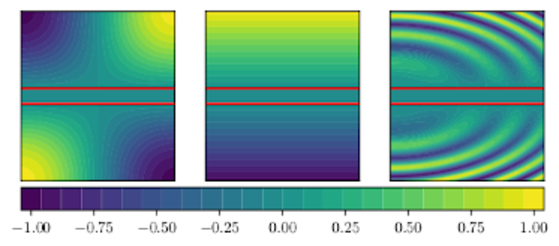
\includegraphics[scale=1.0]{Diagram_GradZeroIllustrations-Scaled.pdf}
	\caption{\label{fig:Diagram_GradZeroIllustrations} Examples illustrating how non-zero gradients of zero can arise, with the region between the red lines representing an edge $I_{jk}$, which has been thickened so one can view the function values along this edge. Despite each of the functions appearing constant along the edge $I_{jk}$, and thus constant to the measure $\lambda_{jk}$, the function is changing in the direction $n_{jk}$ as it crosses $I_{jk}$ and it's behaviour ``off the edge" is unknowable from the perspective of $\lambda_{jk}$. }
\end{figure}
Indeed, the measure $\lambda_{jk}$ is unable to deduce whether (for $x\in I_{jk}$) $u(x+hn_{jk})$ is different from $u(x)$ for $h\neq0$, given the only information it can have about $u$ are its values on $I_{jk}$.
Consequentially, $\lambda_{jk}$ can have no concept of $\pdiff{u}{n_{jk}}$ --- changing the profile of $u$ across the edge $I_{jk}$ does not change $u$ on $I_{jk}$, and consequentially the component of any ``gradient" directed along $n_{jk}$ corresponds to no change in the function $u$ from the perspective of $\lambda_{jk}$, making this component a gradient of zero.
In contrast, the measure $\lambda_{jk}$ can evaluate expressions like $u(x+he_{jk})-u(x)$ --- that is, changes in the function along $I_{jk}$ are detected by the measure $\lambda_{jk}$.
Such changes correspond to $\pdiff{u}{e_{jk}}$ being non-zero, and thus we find that tangential gradients are directed along $e_{jk}$ (and provide a ``derivative" in this direction too).
This also highlights the reason for defining the gradients of zero and tangential gradients as in section \ref{sec:BorelMeasSobSpaces} --- given a tangential gradient $\ktgrad_{\lambda_{jk}}u$, $\lambda_{jk}$ can reconstruct the function $u$ along the edge $I_{jk}$, but cannot determine what $u$ is doing across $I_{jk}$.
Ergo, every function has a gradient that is unique up to a gradient of zero, because there is no way for $\lambda_{jk}$ to determine what $u$ looks like across (and thus outside of) $I_{jk}$.

The above story is similar when considering the tangential gradient of $u$ with respect to the measure $\nu$.
Here, the ``view" of the measure is even more restricted, only being able to view the value of $u$ at the vertices, which are a set of isolated points in $\ddom$.
As such, there is no way for the measure $\nu$ to reconstruct any kind of sensible gradient --- there are no ``nearby" function values $u\bracs{v_j + h x}, x\neq 0$ to compare the value of $u\bracs{v_j}$ to.
The result is corollary \ref{cory:NuTangGradChar}, any gradient must be a gradient of zero, because as far as $\nu$ is concerned, there is no visible change in $u$ in any neighbourhood of $v_j$.
Then, given that $\dddmes$  is just the sum of the measures $\ddmes$ and $\nu$, we find that $\ktgrad_{\dddmes}u$ inherits the behaviours from $\ddmes$ and $\nu$.

\subsection{Derivation of the system \eqref{eq:SingularWaveEqnQGProblem}} \label{ssec:Scalar-QGDerivation}
We can now provide an argument for how a system of the form \eqref{eq:SingularWaveEqnQGProblem} arises from \eqref{eq:SingularScalarWaveEqn}.
Take any $\varphi\in\csmooth{\sqbracs{0,l_{jk}}}$ and let $\phi\in\psmooth{\ddom}$ be such that $\phi\circ r_{jk} = \varphi$ on $\sqbracs{0,l_{jk}}$, with $\supp\phi\cap\graph\subset I_{jk}^{\circ}$.
Recall that the change of variables $r_{jk}$ is affine (see \eqref{eq:EdgeParameterisation}), so in particular this change of variables is invertable.
Testing against such $\phi$ in \eqref{eq:SingularScalarWaveEqn-VariationalForm}, combined with the fact that $\dddmes$ is a sum of the edge measures and point masses at the vertices, and that $\tgrad_{\dddmes}u=\tgrad_{\lambda_{jk}}u$ on the edge $I_{jk}$, equation \eqref{eq:SingularScalarWaveEqn-VariationalForm} implies
\begin{align*}
	0 &= \integral{\ddom}{ \bracs{\tgrad_\ddmes u \cdot \overline{\tgrad\phi} - \omega^2 u\overline{\phi}} }{\ddmes}
	= \integral{I_{jk}}{ \bracs{\tgrad_{\lambda_{jk}}u \cdot \overline{\tgrad\phi} - \omega^2 u^{(jk)}\overline{\phi}} }{\lambda_{jk}} \\
	&= \integral{I_{jk}}{ \clbracs{ \bracs{\bracs{u^{(jk)}}' + \rmi\qm_{jk} u^{(jk)}}\bracs{\overline{\phi}' - \rmi\qm_{jk} \overline{\phi} } - \omega^2 u^{(jk)}\overline{\phi} } }{\lambda_{jk}}.
\end{align*}
Now using the change of variables $r_{jk}$ and denoting $\tilde{u}^{(jk)} = u^{(jk)} \circ r_{jk}$, we arrive at
\begin{align*}
	0 &= \int_{0}^{l_{jk}} \bracs{\bracs{\tilde{u}^{(jk)}}' + \rmi\qm_{jk} \tilde{u}^{(jk)}}\bracs{\overline{\varphi}' - \rmi\qm_{jk} \overline{\varphi} } - \omega^2 \tilde{u}^{(jk)}\overline{\varphi} \ \md y. \\
	\implies
	\int_{0}^{l_{jk}} \bracs{\tilde{u}^{(jk)}}'\overline{\varphi}' \ \md y &=
	\int_{0}^{l_{jk}} \clbracs{ \omega^2\tilde{u}^{(jk)} + 2\rmi\qm_{jk}\bracs{\tilde{u}^{(jk)}}' + \bracs{\rmi\qm_{jk}}^2\tilde{u}^{(jk)} } \overline{\varphi} \ \md y.
\end{align*}
This holds for all $\varphi\in\csmooth{\sqbracs{0,l_{jk}}}$, and thus implies that $\tilde{u}^{(jk)}$ is twice (weakly) differentiable along $\sqbracs{0,l_{jk}}$.
Furthermore, we then obtain the (strong) equation
\begin{align*}
	-\bracs{\diff{}{y} + \rmi\qm_{jk}}^2 \tilde{u}^{(jk)} &= \omega^2 \tilde{u}^{(jk)}, \quad y\in\sqbracs{0,l_{jk}}.
\end{align*}

Now we turn our attention to the derivation of the vertex conditions.
Fix a vertex $v_j\in \vertSet$, and consider functions $\phi\in\psmooth{\ddom}$ with $\supp\phi\cap\graph\subset \mathcal{J}(v_j)\setminus\clbracs{v_j}$ (that is, smooth functions that are only non-zero on $\graph$ close to the vertex $v_j$).
Using the change of variables $r_{jk}$ on each edge and writing $\tilde{u}^{(jk)} = u^{(jk)} \circ r_{jk}$, $\varphi_{jk} = \phi\circ r_{jk}$ for each $k\con j$, we can work from \eqref{eq:SingularScalarWaveEqn-VariationalForm} to obtain
\begin{align*}
	0 &= \sum_{k: \ k\con j} \integral{I_{jk}}{ \bracs{ \tgrad_\ddmes u \cdot \overline{\tgrad\phi} - \omega^2 u\overline{\phi} } }{\lambda_{jk}} 
	+ \integral{\ddom}{ \bracs{ \tgrad_{\dddmes}u\cdot\overline{\tgrad_{\dddmes}\phi}-\omega^2 u\overline{\phi} } }{\massMes} \\
	&= \sum_{k: \ k\con j} \int_{0}^{l_{jk}} \clbracs{ \bracs{\bracs{\tilde{u}^{(jk)}}' + \rmi\qm_{jk} \tilde{u}^{(jk)}}\bracs{\overline{\varphi}_{jk}' - \rmi\qm_{jk} \overline{\varphi}_{jk} } - \omega^2 \tilde{u}^{(jk)}\overline{\varphi}_{jk} } \ \md y \\
	&\qquad + \alpha_j\left.\bracs{ \tgrad_{\dddmes}u\cdot\overline{\tgrad_{\dddmes}\phi}-\omega^2 u\overline{\phi} }\right\vert_{v_j} \\
	&= \sum_{k: \ k\con j} \int_{0}^{l_{jk}} \clbracs{ \bracs{\bracs{\tilde{u}^{(jk)}}' + \rmi\qm_{jk} \tilde{u}^{(jk)}}\bracs{\overline{\varphi}_{jk}' - \rmi\qm_{jk} \overline{\varphi}_{jk} } - \omega^2 \tilde{u}^{(jk)}\overline{\varphi}_{jk} } \ \md y
	 - \alpha_j \omega^2 u\bracs{v_j}\overline{\phi}\bracs{v_j}.
\end{align*}
Here we have used the fact that $\tgrad_{\dddmes}u\bracs{v_j}=0$ (see section \ref{sec:3DGradSobSpaces}).
Given that (from our considerations along the edges) $u$ is twice differentiable on each $I_{jk}$, and $\phi$ is zero at every vertex except $v_j$, it follows that
\begin{align*}
	\alpha_j\omega^2 u\bracs{v_j}\overline{\phi}\bracs{v_j} 
	&= - \sum_{k: \ k\con j} \int_{0}^{l_{jk}} \bracs{ \bracs{\diff{}{x} + \rmi\qm_{jk}}^2 \tilde{u}^{(jk)} +\omega^2 \tilde{u}^{(jk)} }\overline{\varphi}_{jk} \ \md y \\
	&\qquad + \sum_{k: \ k\con j}\overline{\varphi}_{jk}\bracs{v_j}\bracs{\pdiff{}{n} + \rmi\qm_{jk}}\tilde{u}^{(jk)}\bracs{v_j} \\
	&= \overline{\phi}\bracs{v_j}\sum_{k: \ k\con j}\bracs{\pdiff{}{n} + \rmi\qm_{jk}}\tilde{u}^{(jk)}\bracs{v_j}. \labelthis\label{eq:DerivationVertexConditionWeak}
\end{align*}
Given that \eqref{eq:DerivationVertexConditionWeak} holds for every smooth $\varphi$, and that $\varphi_{jk}\bracs{v_j}=\phi\bracs{v_j}$, we arrive at the condition
\begin{align*}
	\alpha_j\omega^2 u\bracs{v_j} &= \sum_{j\con k}\bracs{\pdiff{}{n} + \rmi\qm_{jk}}\tilde{u}^{(jk)}\bracs{v_j}.
\end{align*}

Repeating the argument for each $v_j\in \vertSet$ then provides us with a condition of this form at each vertex.
One should note the presence of $\omega^2$ in this equation, so this is not a Kirchoff condition on the derivatives of the edge functions $u^{(jk)}$, and indicates that the problem we have arrived at is defined through an operator acting in an extended space, as mentioned in section \ref{ssec:DiffOpsOnGraphs}.
The result of theorem \ref{thm:dddmesTangGradImplication} tells us that functions $u\in\gradSobQM{\ddom}{\dddmes}$ are also continuous at each vertex $v_j$, and thus the following problem (precisely \eqref{eq:SingularWaveEqnQGProblem}) has been derived:
\begin{subequations}
	\begin{align*}
		-\bracs{\diff{}{y} + \rmi\qm_{jk}}^2 u^{(jk)} &= \omega^2 u^{(jk)}, \quad &y\in\sqbracs{0,l_{jk}}, \ \forall I_{jk}\in\edgeSet, \tag{\eqref{eq:SingularWaveEqnQGProblem-1} restated} \\
		u \text{ is continuous at } & v_j, \quad &\forall v_j\in\vertSet,  \tag{\eqref{eq:SingularWaveEqnQGProblem-2} restated} \\
		\sum_{j\con k}\bracs{\pdiff{}{n} + \rmi\qm_{jk}}u^{(jk)}\bracs{v_j} &= \omega^2\alpha_j u\bracs{v_j}, \quad &\forall v_j\in\vertSet, \tag{\eqref{eq:SingularWaveEqnQGProblem-3} restated}
	\end{align*}
\end{subequations}
where we henceforth drop the overhead tilde notation and simply write $u^{(jk)}$ for brevity (appealing to the obvious association between $u^{(jk)}$ and $\tilde{u}^{(jk)}$).
As will be made clear in the discussion that follows, the quantum graph problem \eqref{eq:SingularWaveEqnQGProblem} is much easier to handle (than \eqref{eq:SingularScalarWaveEqn}) analytically and numerically thanks to the utility of the $M$-matrix.

Now that we have obtained the system \eqref{eq:SingularWaveEqnQGProblem}, we can affirm our interpretation of the coupling constants $\alpha_j$ as the (limit of the) ratio of vertex volume $V_{\mathrm{vertex}}$ to edge volume $V_{\mathrm{edge}}$ that was described in section \ref{ssec:Intro-ThinStructures}.
As can clearly be seen from \eqref{eq:SingularWaveEqnQGProblem-3}, when $\alpha_j$ is non-zero and finite, we obtain Wentzell conditions between the incoming derivatives to the vertex $v_j$.
This is precisely the boundary condition we would obtain in the zero-thickness limit for the (Neumann) Laplacian on a thickened graph, provided the ratio $\frac{V_{\mathrm{vertex}}}{V_{\mathrm{edge}}}\rightarrow\alpha_j$ as the thickness of the structure tended to zero.
Moreover, notice that if $\alpha_j=0$ in \eqref{eq:SingularWaveEqnQGProblem-3}, we obtain an exact Kirchoff condition at the vertex $v_j$, along with continuity of the incoming edge functions --- precisely the case when $V_{\mathrm{vertex}}\ll V_{\mathrm{edge}}$.
Finally, if one divides through by $\alpha_j$ in \eqref{eq:SingularWaveEqnQGProblem-3} and takes a formal limit as $\alpha_j\rightarrow\infty$, the resulting system imposes homogeneous Dirichlet boundary conditions on the solution $u$ at $v_j$ --- corresponding to the conditions obtained in the limiting case $V_{\mathrm{vertex}}\gg V_{\mathrm{edge}}$.
We can also predict the resulting problems of thickened graphs that possess a mixture of vertex and edge volumes; that is when a thickened graph $\mathcal{G}_{\delta}$ of $\graph$ is such that $V_{\mathrm{edge}}\bracs{\delta}$ is the same for every (thickened) edge, yet the scaling of the volume of the thickened vertices $V_{v_j}\bracs{\delta}, v_j\in\vertSet$ with $\delta$ changes between vertices.
Letting $\alpha_j = \lim_{\delta\rightarrow0}\frac{V_{v_j}}{V_{\mathrm{edge}}}$ (where we formally allow $\alpha_j=\infty$) for each $v_j$, our consideration of singular measures and the variational problem \eqref{eq:SingularScalarWaveEqn} predicts that the resulting system will be realisable as the following quantum graph problem:
\begin{subequations}
	\begin{align*}
		-\bracs{\diff{}{y} + \rmi\qm_{jk}}^2 u^{(jk)} &= \omega^2 u^{(jk)}, \quad & y\in\sqbracs{0,l_{jk}}, \ \forall I_{jk}\in\edgeSet, \\
		u \text{ is continuous at } & v_j, \quad &\forall v_j\in\vertSet, \\
		\sum_{j\con k}\bracs{\pdiff{}{n} + \rmi\qm_{jk}}u^{(jk)}\bracs{v_j} &= \omega^2\alpha_j u\bracs{v_j}, \quad &\forall v_j\in\vertSet, \ \alpha_j\in\bracs{0,\infty}, \\
		\sum_{j\con k}\bracs{\pdiff{}{n} + \rmi\qm_{jk}}u^{(jk)}\bracs{v_j} &= 0, \quad &\forall v_j\in\vertSet, \ \alpha_j = 0, \\
		u\bracs{v_j} &= 0, \quad &\forall v_j\in\vertSet, \ \alpha_j = \infty.
	\end{align*}
\end{subequations}
We also remark that, for a graph with $\alpha_j<\infty$ for every $v_j$, our approach via the $M$-matrix (section \ref{sec:ScalarDiscussion}) for determining the spectrum of the above problem can be employed.

\subsection{The relation between $\tgradSob{\ddom}{\dddmes}$ and extended spaces} \label{ssec:ExtendedSpaces}
As we have already discussed, the problem \eqref{eq:SingularWaveEqnQGProblem} coincides with the problems that arise in the zero-thickness limit of thin-structures.
Indeed, the system \eqref{eq:SingularWaveEqnQGProblem} corresponds to the operator $\mathcal{A}_{\mathrm{ext}}$ that acts in the \emph{extended space}
\begin{align*}
	\dom\mathcal{A}_{\mathrm{ext}} 
	&= \clbracs{ (u, \beta) \setVert u\in H^2\bracs{\graph}, \ u \text{ is continuous at each } v_j\in\vertSet, \ \beta_j=\alpha_j u(v_j) } \\
	& \subset L^2\bracs{\graph}\oplus\complex^{\abs{\vertSet}}.
\end{align*}
The element $\bracs{u,\beta}$ is a $\abs{\edgeSet}+\abs{\vertSet}$ ``vector" (more precisely, tuple) consisting of the edge functions $u^{(jk)}$, followed by the (scaled) vertex values $\beta_j$, which we shall write as
\begin{align*}
	\begin{pmatrix} u \\ \beta \end{pmatrix}
	&= \begin{pmatrix} \clbracs{u^{(jk)}}_{I_{jk}\in\edgeSet} \\ \clbracs{\beta_j}_{v_j\in\vertSet} \end{pmatrix}.
\end{align*}
The action of $\mathcal{A}_{\mathrm{ext}}$ defined as
\begin{align*}
	\mathcal{A}_{\mathrm{ext}} \begin{pmatrix} u \\ \beta \end{pmatrix}
	&= 
	\begin{pmatrix}
		\clbracs{-\bracs{\diff{}{y}+\rmi\qm_{jk}}^2 u^{(jk)}}_{I_{jk}\in\edgeSet} \\ 
		\clbracs{\sum_{j\con k}\bracs{ \pdiff{}{n} + \rmi\qm_{jk} }u^{(jk)}(v_j)}_{v_j\in\vertSet}
	\end{pmatrix},
\end{align*}
the space $L^2\bracs{\graph}\oplus\complex^{\abs{\vertSet}}$ is the extended space, and $\mathcal{A}_{\mathrm{ext}}$ the Strauss extension for the problem \eqref{eq:SingularWaveEqnQGProblem}.

It is clear that the operators $\mathcal{A}_{\mathrm{ext}}$ and $-\laplacian_{\dddmes}^{\qm}$ possess the same spectrum and eigenfunctions, by virtue of theorem \ref{thm:CharOfSobSpaces}.
Now let $f\in L^2\bracs{\graph}\oplus\complex^{\abs{\vertSet}} \cong \ltwo{\ddom}{\dddmes}$.
Setting aside questions of solubility for the time being, a solution to the problem $\mathcal{A}_{\mathrm{ext}}u=f$ is also guaranteed to provide a solution to $-\laplacian_{\qm}^{\dddmes}u=f$ and vice-versa through this theorem.
The converse also assured upon realising the problem $-\laplacian_{\qm}^{\dddmes}u=f$ can be written in the form \eqref{eq:SingularWaveEqnQGProblem}\footnote{The fact that $f\in\ltwo{\ddom}{\dddmes}$ is important here, as it provides enough regularity for $u$ to be an element of $H^2\bracs{\graph}$.}, except replacing $\omega^2 u$ with $f$ in \eqref{eq:SingularWaveEqnQGProblem-1} and $\omega^2\alpha_j u(v_j)$ with $\alpha_j f(v_j)$ in \eqref{eq:SingularWaveEqnQGProblem-3}.
Our approach via singular measures has resulted in the immediate construction of the extended space \emph{and corresponding operator} one obtains in the zero-thickness limit of thin-structure problems.
Within the context of the acoustic approximation we already knew what these limits where, however our original formulation provides a method of defining this limiting problem by appealing to the geometry.
This also presents an opportunity we look to investigate going forward; the non-classical Sobolev spaces and variational problems provide us with a method of defining (up to isomorphism) the spaces and problems that may correspond to the --- presently unknown --- ``limits" of other thin-structure problems.

\section{General formula for the $M$-matrix of a finite period graph} \label{sec:ScalarDiscussion}
Having obtained the quantum graph problem \eqref{eq:SingularWaveEqnQGProblem}, we turn our attention to determining the eigenvalues $z := \omega^2$.
The advantage of \eqref{eq:SingularWaveEqnQGProblem} over working directly with \eqref{eq:SingularScalarWaveEqnWholeSpace} is that we can now use the $M$-matrix (introduced in section \ref{ssec:MMatrix}) as a tool in our analysis.
In this section we contextualise the theory introduced in section \ref{sec:QuantumGraphs}, and in particular section \ref{ssec:MMatrix}, showing how it is employed for studying the spectrum of \eqref{eq:SingularScalarWaveEqnWholeSpace}.
In doing so, we provide a general formula for the $M$-matrix of a finite period graph on which \eqref{eq:SingularWaveEqnQGProblem} is posed.
We will follow up on this in section \ref{sec:Examples}, where we provide some explicit examples of quantum graph problems that can be solved by employing the $M$-matrix in the manner discussed below.

\subsection{General formula for the $M$-matrix} \label{ssec:MMatrixResult}
One of the foremost advantages of the $M$-matrix is that we can explicitly (and analytically) compute its entries for any (finite period) metric graph $\graph$ on which the system \eqref{eq:SingularWaveEqnQGProblem} is posed.
We also break from assumption \ref{ass:MeasTheoryProblemSetup}, and allow for the period graph to include looping edges (edges whose endpoints correspond to same vertex), since such loops do not effect the (procedure in the) proof of the result.
The inclusion of looping edges is mostly for completeness, since when we come to use the $M$-matrix to determine the eigenvalues of \eqref{eq:SingularWaveEqnQGProblem}, we will want to introduce ``artificial vertices" (section \ref{ssec:ArtificialVertices}) to break these loops.
The following proposition provides the entries of the $M$-matrix.
\begin{prop}[$M$-matrix entries] \label{prop:M-MatrixEntries}
	Let $\graph=\bracs{\vertSet,\edgeSet}$ be an embedded graph on which the problem \eqref{eq:SingularWaveEqnQGProblem} is posed.
	Suppose that $\dmap u = e_k$ where $e_k$ is the $k$\textsuperscript{th} canonical unit vector in $\complex^{\abs{\vertSet}}$.
	Then the $j$\textsuperscript{th} entry of $\nmap u$, and hence the $jk$\textsuperscript{th} entry in the $M$-matrix, is given by
	\begin{align*}
		\bracs{\nmap u}_j &= 
		\begin{cases}
			0,	
			& j \not\con k, \\[5pt]
			\sum_{j\conLeft k} \omega \e^{\rmi\qm_{jk}l_{jk}} \csc\bracs{l_{jk}\omega} 
			+ \sum_{j\conRight k} \omega \e^{-\rmi\qm_{kj}l_{kj}} \csc\bracs{l_{kj}\omega},
			& j\neq k, \ j\con k, \\[5pt]
			- \sum_{\substack{j\con l \\ j\neq l}} \omega\cot\bracs{l_{jl}\omega}
			- 2\omega\sum_{j\conLeft j} \clbracs{ \cot\bracs{l_{jj}\omega} - \cos\bracs{\qm_{jj}l_{jj}}\csc\bracs{l_{jj}\omega} },
			& j=k.
		\end{cases}
	\end{align*}
\end{prop}
Note the choice of $j\conLeft j$ in the contributions from loops is simply a convention, $j\conRight j$ is equivalent here.
Also recall the convention for summing over $j\con k$:
\begin{align*}
	\sum_{j\con k} \omega\cot\bracs{l_{jk}\omega} &= \sum_{j\conLeft k} \omega\cot\bracs{l_{jk}\omega}	+ \sum_{j\conRight k} \omega\cot\bracs{l_{kj}\omega}
\end{align*}
\begin{proof}
	The proof below is an explicit computation, similar to that in \cite{ershova2014isospectrality} with adjustments for the dependence on $\qm$.
	
	We first write the general form of the edge solution $u^{(jk)}$ from \eqref{eq:SingularWaveEqnQGProblem-1}:
	\begin{align} \label{eq:EdgeEqnGeneralSolution}
		u^{(jk)} &= \e^{-\rmi\qm_{jk}t}\bracs{ C_{+}^{(jk)}\e^{-\rmi\omega x} + C_{-}^{(jk)}\e^{\rmi\omega x} },
		\quad C_{+}^{(jk)}, C_{-}^{(jk)}\in\complex.
	\end{align}
	Since the $M$-matrix maps $\complex^{\abs{\vertSet}}$ to $\complex^{\abs{\vertSet}}$, it is sufficient to determine its action on the canonical basis of $\complex^{\abs{\vertSet}}$.
	So for each fixed $k\in\clbracs{1,...,\abs{\vertSet}}$ we set $\dmap u = e_k$.
	This provides us with sufficient Dirichlet data to solve \eqref{eq:SingularWaveEqnQGProblem-1} on each edge and eliminate the constants $C_{+}^{(jk)}$, $C_{-}^{(jk)}$ in \eqref{eq:EdgeEqnGeneralSolution}, obtaining
	\begin{align*}
		j\not\con k &\implies
		\begin{cases}
			u_{jk}(x) = 0, \\
			u_{kj}(x) = 0,
		\end{cases} \\
		j\neq k, \ j\con k &\implies
		\begin{cases}
			u_{jk}(x) = \e^{-\rmi\qm_{jk}\bracs{x-l_{jk}}}\csc\bracs{\omega l_{jk}}\sin\bracs{\omega x}, \\
			u_{kj}(x) = \e^{-\rmi\qm_{kj}x}\csc\bracs{\omega l_{kj}}\sin\bracs{\omega \bracs{l_{kj}-x}},
		\end{cases} \\
		j = k &\implies 
		\begin{cases}
			u_{jj}(t) = \e^{-\rmi\qm_{jj}x} \bracs{ \e^{-\rmi\omega x} + \sqbracs{\e^{\rmi\qm_{jj}l_{jj}}-\e^{-\rmi\omega l_{jj}}}\csc\bracs{\omega l_{jj}}\sin\bracs{\omega x}  },
		\end{cases}
	\end{align*}
	This in turn enables us to explicitly differentiate the expressions for $u_{jk}$, and read off the values of $\bracs{\pdiff{}{n}+\rmi\qm_{jk}}u_{jk}$ at the vertices.
	In the case $j\not\con k$, we obviously get zero contribution from the edges $I_{jk}$ and $I_{kj}$.
	The case $j\neq k, \ j\con k$, yields the following contributions from the edges $I_{jk}$ and $I_{kj}$:
	\begin{align*}
		\bracs{\pdiff{}{n}+\rmi\qm_{jk}}u^{(jk)}\bracs{v_j} = -\omega \e^{\rmi\qm_{jk}l_{jk}}\csc\bracs{\omega l_{jk}}, 
		&\qquad \bracs{\pdiff{}{n}+\rmi\qm_{jk}}u^{(jk)}\bracs{v_k} = \omega\cot\bracs{\omega l_{jk}}, \\
		\bracs{\pdiff{}{n}+\rmi\qm_{kj}}u^{(kj)}\bracs{v_j} = -\omega \e^{-\rmi\qm_{kj}l_{kj}}\csc\bracs{\omega l_{kj}}, 
		&\qquad \bracs{\pdiff{}{n}+\rmi\qm_{kj}}u^{(kj)}\bracs{v_k} = \omega\cot\bracs{\omega l_{kj}}.
	\end{align*}
	Finally, when considering the case $j=k$, the contribution to $\bracs{\nmap u}_j$ from loops $I_{jj}$ in the graph also requires us to compute
	\begin{align*}
		-\lim_{x\rightarrow0}\bracs{\bracs{u^{(jj)}}'+i\qm_{jj}u^{(jj)}}(x) + \lim_{x\rightarrow l_{jj}} & \bracs{\bracs{u^{(jj)}}'+i\qm_{jj}u^{(jj)}}(x) \\
		&\qquad = 2\omega\bigl( \cot\bracs{\omega l_{jj}} - \cos\bracs{\qm_{jj}l_{jj}}\csc\bracs{\omega l_{jj}} \bigr).	
	\end{align*}
	We then use the formula
	\begin{align*}
		\bracs{\nmap u}_j &= -\sum_{j\con l} \bracs{\pdiff{}{n}+\rmi\qm_{jl}}u^{(jl)}\bracs{v_j},
	\end{align*}
	which yields the desired result.
\end{proof}

Proposition \ref{prop:M-MatrixEntries} also explicitly demonstrates that the $M$-matrix (in the context of \eqref{eq:SingularWaveEqnQGProblem}) is parametrised by $\qm$, and so we shall denote it by $M_{\qm}$ henceforth.
The dependence of $M_\qm$ on $\qm$ is due to our decision to specify our singular structure (comprising the domain in which \eqref{eq:SingularScalarWaveEqnWholeSpace} was posed) as an embedded, periodic metric graph and then apply the Gelfand transform (see section \ref{ssec:MMatrix}).
In the following section, we continue our analysis of the $M$-matrix and outline how it can be used to recover the eigenvalues $z=\omega^2$ of \eqref{eq:SingularWaveEqnQGProblem}, and thus \eqref{eq:SingularScalarWaveEqnWholeSpace}.

\subsection{Consequences of Proposition \ref{prop:M-MatrixEntries}} \label{ssec:MMatrixConsequences}
Whilst proposition \ref{prop:M-MatrixEntries} provides an explicit form for the entries of the $M$-matrix,  it is not the most convenient when looking for a method for determining the spectrum of \eqref{eq:SingularWaveEqnQGProblem}.
Proposition \ref{prop:M-MatrixEntries} shows that $M_\qm$ is meromorphic, and thus has the following decomposition:
\begin{cory} \label{cory:M-MatrixEntriesNoPoles}
	Let $G^{(1)}_\qm\bracs{\omega}$ have entries defined by
	\begin{align*}
		\bracs{G^{(1)}_\qm}_{jk} &= 
		\begin{cases}
			\!\begin{aligned}
				&0,
			\end{aligned}			
			& j \not\con k, \\
			\!\begin{aligned}
				&\sum_{j\conLeft k} \bracs{ \e^{\rmi\qm_{jk}l_{jk}} \prod_{v_l\in\vertSet}\prod_{\substack{ l\conLeft m \\ \bracs{l,m} \neq \bracs{j,k} }}\sin\bracs{l_{lm}\omega} }
				\\ &\quad + \sum_{j\conRight k} \bracs{ \e^{-\rmi\qm_{kj}l_{kj}} \prod_{v_l\in\vertSet}\prod_{\substack{l\conLeft m \\ \bracs{l,m} \neq \bracs{k,j} }}\sin\bracs{l_{lm}\omega} },
			\end{aligned}
			& j\neq k, \ j\con k, \\
			\!\begin{aligned}
				&- \sum_{\substack{j\con l \\ j\neq l}} \bracs{ \cos\bracs{l_{jl}\omega}\prod_{v_m\in\vertSet}\prod_{\substack{ m\conLeft n \\ \bracs{m,n}\neq\bracs{j,l} }}\sin\bracs{l_{mn}\omega} }
				\\ &\quad - 2\sum_{j\conLeft j} \bracs{ \sqbracs{ \prod_{v_l\in\vertSet}\prod_{\substack{l\conLeft m \\ \bracs{l,m}\neq\bracs{j,j} }}\sin\bracs{l_{lm}\omega} }\bigl[ \cos\bracs{l_{jj}\omega} - \cos\bracs{\qm_{jj}l_{jj}} \bigr] },
			\end{aligned}
			& j=k,
		\end{cases}
	\end{align*}
	and set
	\begin{align*}
		G^{(2)}\bracs{\omega} &= \prod_{v_j\in\vertSet} \prod_{j\conLeft k}\sin\bracs{l_{jk}\omega}.
	\end{align*}
	Further define
	\begin{align*}
		H^{(1)}_{\qm}(z) &:= 
		\begin{cases} 
			\omega G_\qm^{(1)}(\omega), & \abs{\edgeSet} \text{ is even}, \\
			G_\qm^{(1)}(\omega), & \abs{\edgeSet} \text{ is odd},
		\end{cases} \\
		H^{(2)}(z) &:=
		\begin{cases}
			G^{(2)}(\omega), & \abs{\edgeSet} \text{ is even}, \\
			\omega^{-1} G^{(2)}(\omega), & \abs{\edgeSet} \text{ is odd}.
		\end{cases}
	\end{align*}
	Then the functions $H^{(1)}_{\qm}(z)$ and $H^{(2)}(z)$ are analytic in $z:=\omega^2$ and we have
	\begin{align*}
		M_\qm\bracs{z} &= \bracs{ H^{(2)}\bracs{z} }^{-1} H^{(1)}_\qm\bracs{z}.
	\end{align*}
\end{cory}
The product notation should be understood analogously to the summation notation over $j\con k$ introduced in section \ref{sec:QuantumGraphs}.
The zeros of $H^{(2)}$ exactly coincide with the poles of $M_\qm$, both $H^{(1)}_\qm$ and $H^{(2)}$ are analytic, and the matrix $H^{(1)}_\qm$ even has its entry at position $jk$ bounded (uniformly in $\omega$) by the number of (direct) connections between $v_j$ and $v_k$.

Recall that (section \ref{ssec:MMatrix}) we need to determine those $z$ for which the matrix $M_\qm(z)-B(z)$ has at least one zero eigenvalue, where we have $B(z) = -z\alpha$.
Note the dependence of $B$ on $z$ --- this was raised in section \ref{ssec:DiffOpsOnGraphs}.
Now let $\beta_j\bracs{z}, j\in\clbracs{1,...,\abs{\vertSet}}$ denote the eigenvalue branches of the matrix $M_\qm(z)-B(z)$.
Also set $\mathfrak{M}_\qm(z) = H^{(1)}_\qm(z) - H^{(2)}(z)B(z)$, and let $\widetilde{\beta}_j\bracs{z}, j\in\clbracs{1,...,\abs{\vertSet}}$ denote the eigenvalue branches of $\mathfrak{M}_\qm$.
The matrix $\mathfrak{M}_\qm$ is analytic, and so has at least one zero eigenvalue at those $z$ for which there exists a $w\in\complex^{\abs{\vertSet}}\setminus\clbracs{0}$ such that
\begin{align} \label{eq:QGGenEvalSolveNoPoles}
	\mathfrak{M}_\qm\bracs{z}w = 0.
\end{align}
We could also chose to determine these $z$ via solution to 
\begin{align} \label{eq:QGDetSolveCondition}
	\det\mathfrak{M}_\qm\bracs{z} &= 0,
\end{align}
the merits of each approach (via \eqref{eq:QGGenEvalSolveNoPoles} or \eqref{eq:QGDetSolveCondition}) we will discuss in section \ref{ssec:ApproachConsiderations}.
If $z_0$ solves \eqref{eq:QGGenEvalSolveNoPoles} (or equivalently \eqref{eq:QGDetSolveCondition}), then $M_{\qm}\bracs{z_0}-B\bracs{z_0}$ has a zero eigenvalue when
\begin{align} \label{eq:EigenvalueBranchLimit}
	\lim_{z\rightarrow z_0} \beta_j\bracs{z} = \lim_{z\rightarrow z_0} \bracs{ H^{(2)}\bracs{z} }^{-1} \widetilde{\beta}_j\bracs{z} = 0
\end{align}
for at least one $j$ with $\widetilde{\beta}_j\bracs{z_0}=0$.
Checking the limit in \eqref{eq:EigenvalueBranchLimit} is not necessary for all solutions $z_0$ to \eqref{eq:QGDetSolveCondition}; provided that $H^{(2)}\bracs{z_0}\neq 0$, which by corollary \ref{cory:M-MatrixEntriesNoPoles} occurs when
\begin{align*}
	z_0 \neq \bracs{ \frac{n\pi}{l_{jk}} }^2, \quad j\conLeft k, \ n\in\naturals_{0},
\end{align*}
the limit in \eqref{eq:EigenvalueBranchLimit} is clearly zero, and so $z_0$ belongs to the spectrum of \eqref{eq:SingularWaveEqnQGProblem}.
As we will discuss in section \ref{ssec:ApproachConsiderations}, checking the limit \eqref{eq:EigenvalueBranchLimit} may not be necessary at all, given known results about the spectra of periodic quantum graph problems.
Considerations concerning which of the two equations (\eqref{eq:QGGenEvalSolveNoPoles} or \eqref{eq:QGDetSolveCondition}) should be used for determining the spectrum $\sigma_\qm$ are also discussed in section \ref{ssec:ApproachConsiderations}.
In any event, \eqref{eq:SingularScalarWaveEqnWholeSpace} has now been reduced to a more accessible (family of) matrix-eigenvalue problems for $\mathfrak{M}_\qm$.

\subsection{Artificial Vertices and Splitting Edges} \label{ssec:ArtificialVertices}
As noted in section section \ref{ssec:MMatrix}, it is required that the underlying graph $\graph$ contains no looping edges and has all edge-lengths pairwise irrationally-related.
Failure to ensure that this condition is met may result in the ``loss" of certain eigenvalues when using the $M$-matrix to determine the spectrum of \eqref{eq:SingularWaveEqnQGProblem} --- these are highlighted explicitly in section \ref{ssec:Example1DLoop}.
Of course, the graphs motivated by physical applications generally do not adhere to these restrictions, so it is necessary to introduce ``artificial" or ``dummy" vertices.
These artificial vertices ``split" edges of the original graph, removing any loops and ensuring all (new) edges have irrationally-related lengths.

Introducing an artificial vertex to split an edge is as intuitive as it sounds --- suppose $\graph=\bracs{\vertSet, \edgeSet}$ and one wishes to ``split" the edge $I_{jk}$ (where it may be the case that $j=k$).
Place a vertex $v_l$ at some point along the edge $I_{jk}$, and replace $I_{jk}$ with the edges $I_{jl}$ and $I_{lk}$, to obtain a new graph $\graph^*$.
The total length of the edges must be preserved, so $\abs{I_{jk}} = \abs{I_{jl}}+\abs{I_{lk}}$, but the lengths of the new edges should be chosen in accordance with the requirements above in mind.
Furthermore, a zero coupling constant should be placed at the artificial vertex $v_l$ --- this ensures matching of the solution $u$ and its derivative at the artificial vertex, as would have been the case along the original edge if it had not been split.
The quasi-momentum parameters should also satisfy $\qm_{jl}=\qm_{lk}=\qm_{jk}$ (although this is a by-product of having straight edges, see assumption \ref{ass:MeasTheoryProblemSetup}).
This ensures (via \eqref{eq:SingularWaveEqnQGProblem-2} and \eqref{eq:SingularWaveEqnQGProblem-3}) that any eigenvalues $\omega^2$ of \eqref{eq:SingularWaveEqnQGProblem} on $\graph^*$ are also eigenvalues of \eqref{eq:SingularWaveEqnQGProblem} on $\graph$, with the eigenfunction $u^{(jk)}$ being related to $u^{(jl)}$ and $u^{(lk)}$ in the obvious manner.
This process can be iterated, splitting edges iteratively to remove rational-relations between edge lengths, and any loops themselves.
Doing so means that any graph representing a singular-structure can now be treated in the manner described in section \ref{ssec:MMatrixConsequences}.

\subsection{Considerations for the Approach to Solving \eqref{eq:QGGenEvalSolveNoPoles} or \eqref{eq:QGDetSolveCondition}} \label{ssec:ApproachConsiderations}
In this section we briefly discuss some considerations for recovering the spectrum of \eqref{eq:SingularScalarWaveEqnWholeSpace} (which we denote by $\sigma$), and the merits of determining the spectrum of \eqref{eq:SingularWaveEqnQGProblem} (denoted $\sigma_\qm$) via \eqref{eq:QGGenEvalSolveNoPoles} or \eqref{eq:QGDetSolveCondition}.
Recall that our use of the Gelfand transform informs us that $\sigma = \bigcup_{\qm}\sigma_{\qm}$.
We also take as a baseline that one has to hand an appropriate numerical scheme for handling the generalised eigenvalue problem \eqref{eq:QGGenEvalSolveNoPoles} (a good introduction to which can be found in \cite{guttel2017nonlinear}), and so do not delve into the details of how such an algorithm would operate.
It is however worth mentioning that $\mathfrak{M}_\qm$ is Hermitian, from which most numerical schemes benefit.

There are also several known results concerning the spectra of (periodic) quantum graphs, and here we highlight those most relevant to our context. 
A detailed discussion of the spectral structure of (periodic) quantum graphs, including statements (and proofs) of the results cited here, can be found in \cite[Chapter 4]{berkolaiko2013introduction}.
Foremost, it is known that there exist real numbers $a_j, b_j, j\in\naturals$ such that $\sigma = \bigcup_{j\in\naturals}\sqbracs{a_j,b_j}$ --- $\sigma$ is said to have a \emph{band-gap structure} or \emph{representation} \cite[Chapter 4.3]{berkolaiko2013introduction} if this is the case.
The \emph{spectral bands} are the intervals $I_j=\sqbracs{a_j,b_j}, \ j\in\naturals$, with the regions between $b_j$ and $a_{j+1}$ being referred to as \emph{spectral gaps}, where there are no eigenvalues.
For this reason the points $a_j$ and $b_j$ sometimes referred to as the \emph{spectral edges}, and in general $a_j\rightarrow\infty$ as $j\rightarrow\infty$.
Knowing that $\sigma$ has a band-gap representation is particularly useful when attempting to use either \eqref{eq:QGGenEvalSolveNoPoles} or \eqref{eq:QGDetSolveCondition} to determine it, which we will touch on shortly.
Other notable results are that $\sigma$ has no singular continuous part (\cite[Chapter 4.4]{berkolaiko2013introduction}) but may have non-empty pure-point part (\cite[Chapter 4.5]{berkolaiko2013introduction}) --- a non-empty pure-point spectrum implies the existence of a compactly supported eigenfunction for the graphs considered in this work.

Using corollary \ref{cory:M-MatrixEntriesNoPoles}, the following proposition can be proved.
\begin{prop} \label{prop:MMatrixDetForm}
	Given a graph $\graph = \bracs{\vertSet, \edgeSet}$, with the lengths of the edges of $\graph$ pairwise-irrationally related, there exists a function $F\bracs{\qm,\omega}$ such that
	\begin{align} \label{eq:MMatrixDetForm}
		\det\mathfrak{M}_\qm\bracs{\omega^2} = \bracs{ \omega H^{(2)}\bracs{\omega^2} }^{\abs{\vertSet}-2} F\bracs{\qm,\omega}.
	\end{align}
	Furthermore, $F\bracs{\qm,\omega}$ is analytic in both its arguments.
\end{prop}
The proof of this result can be found in section \ref{sec:ProofOfProp}, but essentially involves counting the number of times a given factor can appear in the expression for the determinant.
The prefactor $\bracs{ \omega H^{(2)}\bracs{\omega^2} }^{\abs{\vertSet}-2}$ informs us that checking \eqref{eq:EigenvalueBranchLimit} will be necessary for all the roots of $H^{(2)}$.
The set $F_0 := \clbracs{\omega \setVert \exists\qm \text{ s.t. }F\bracs{\qm, \omega}=0}$ then determines the remainder of $\sigma$ --- so in particular, the function $F$ determines the ``width" of the spectral bands, or the vast majority of the spectrum.
Finding $\sigma$ (up to checking roots of $H^{(2)}$) now becomes a question of obtaining $F_0$ efficiently.
One can always take the ``brute-force" approach: compute $F_0^{\qm} := \clbracs{\omega \setVert F\bracs{\qm, \omega}=0}$ for each $\qm$ (or for each $\qm$ in a suitable mesh if working numerically), and then take the union over $\qm$ to obtain $F_0$.
This is computationally expensive (both numerically and analytically) and ``brute force" should only be a last resort, so we highlight some alternatives.

If we can write $F\bracs{\qm,\omega} = F_1\bracs{\qm} - F_2\bracs{\omega}$ for continuous $F_1$ and $F_2$, then \eqref{eq:QGDetSolveCondition} implies $F_0$ can be found simply by examining
\begin{align*}
	\min_{\qm}\clbracs{F_1(\qm)} \leq F_2\bracs{\omega} \leq \max_{\qm}\clbracs{F_1(\qm)},
\end{align*} 
although such a separation of $F$ will not generally be possible, and this also relies finding an analytic expression for $\det\mathfrak{M}_\qm$.
One can always ask the more general question of whether, given the knowledge that $\sigma$ has a band-gap structure, an alternative to finding all $\omega\in F_0$ is to only compute the spectral edges $a_j, b_j$ and then reconstruct $F_0$ from them.
It is known for (second order) periodic PDE problems that the edges of the spectrum occur at the symmetry values of the quasi-momentum --- those values of $\qm$ which correspond to the periodic and anti-periodic problems (in each axis direction) on the unit cell.
If the above statement were true for (periodic) quantum graphs, then the dimensionality of the problem of computing $F_0$ (hence $\sigma$) could be reliably reduced to determining $F_0^\qm$ for the aforementioned symmetry values of $\qm$.
However as discussed in \cite[Chapter 4.6]{berkolaiko2013introduction}, whilst this has been experimentally observed to be true for most physically motivated quantum graph topologies, but is in fact untrue in general.
Despite this, \cite[Chapter 4.6]{berkolaiko2013introduction} remarks that adopting this approach of assuming the spectral edges lie at the symmetry points of the quasi-momentum doesn't often lead to errors in practice, although it is unclear why.
The ``working hypothesis" or ``rule of thumb" is that the period graph needs to be made (very) asymmetric to move the spectral edges away from the symmetry points of the quasi-momentum, and since most physical structures of interest display symmetries in their unit cells, the statement appears to be ``true in practice".

The discussion in the previous paragraph focused on obtaining $\sigma$ and $\sigma_\qm$ via the solution to \eqref{eq:QGDetSolveCondition}.
Here we discuss some situations where it is more appropriate to use \eqref{eq:QGGenEvalSolveNoPoles} to determine $\sigma_{\qm}$ (and thus $\sigma$), although the discussion concerning the determination of the spectral edges $a_j, b_j$ is still applicable to solution methods that work via \eqref{eq:QGGenEvalSolveNoPoles}.
If one is looking to numerically solve for $\sigma_\qm$, then the default choice should be to solve the generalised eigenvalue problem \eqref{eq:QGGenEvalSolveNoPoles}.
Eigenvalue-finding schemes usually benefit from knowing that $\mathfrak{M}_\qm$ is Hermitian, and \eqref{eq:QGGenEvalSolveNoPoles} avoids having to work with $\det\mathfrak{M}_\qm$ --- which is generally advisable when handling matrices numerically. 
On the other hand, if one is willing to perform some analytic work, solving via \eqref{eq:QGDetSolveCondition} offers the possibility of finding an expression for $\det\mathfrak{M}_\qm$ in terms of rational functions ($\sin, \cos$, etc) on which less expensive numerical schemes can be used, or determining $\sigma_\qm$ outright.
As such, the choice of approach largely depends on how willing the solver is to work analytically with $\mathfrak{M}_\qm$.
With this in mind, corollary \ref{cory:M-MatrixEntriesNoPoles} tells us that the complexity of the entry of $\bracs{\mathfrak{M}_\qm}_{jk}$ depends on the number of edges between the vertices $v_j$ and $v_k$, whilst the complexity of the diagonal entries depends on the degree of the vertex $v_j$.
Furthermore, the number of vertices in the graph determines the dimensions of $\mathfrak{M}_\qm$, and the sparsity of $\mathfrak{M}_\qm$ depends on the number of pairs of vertices that are not (directly) connected by an edge.
This leads to the colloquial rule that solving \eqref{eq:QGDetSolveCondition} (analytically) is generally manageable for graphs with a ``small number" of edges and/or vertices, whilst graphs with a large number of edges and/or vertices often warrant solution via \eqref{eq:QGGenEvalSolveNoPoles}.
Of course, the cut-off for the terms ``small number" and ``large number" will depend on the person (or program) solving the problem themselves!
With this in mind, the ratio $\frac{\abs{\edgeSet}}{\abs{\vertSet}}$ can also be a good indicator the ``sparsity" of $\mathfrak{M}_\qm$, and thus how difficult $\mathfrak{M}_\qm$ will be to work with.
If $\frac{\abs{\edgeSet}}{\abs{\vertSet}}\approx 1$, then the number of non-zero entries in any row (or column) of $\mathfrak{M}_\qm$ should be approximately 2 --- the diagonal entry plus the entry corresponding to the expected single connection of this vertex.
At the extremes, $\frac{\abs{\edgeSet}}{\abs{\vertSet}}\approx 0$ corresponds to an almost-diagonal $\mathfrak{M}_\qm$, whilst $\frac{\abs{\edgeSet}}{\abs{\vertSet}}\approx \abs{\vertSet}$ corresponds to an almost-dense $\mathfrak{M}_\qm$.
A sparse $\mathfrak{M}_\qm$ can be easy to handle analytically and efficient to work with numerically, even if $\abs{\vertSet}$ is relatively large.
For denser $\mathfrak{M}_\qm$, one likely begins to lean toward numerical schemes, as the expressions involved in \eqref{eq:QGDetSolveCondition} becomes increasingly cumbersome.

\section{Dispersion relations for concrete graph topologies} \label{sec:ScalarExamples}
In this section we provide examples to demonstrate how the spectrum of the problem \eqref{eq:SingularScalarWaveEqnWholeSpace} is obtained via the analysis of the $M$-matrix for the quantum graph problem \eqref{eq:SingularWaveEqnQGProblem}.
The examples are chosen to highlight the methodology and some of the remarks discussed in sections \ref{sec:QuantumGraphs} and \ref{sec:ScalarDiscussion}.

\subsection{One-Dimensional Loop} \label{ssec:Example1DLoop}
We begin with the simplest example: a ``chain" of vertices that is periodic in one direction, to demonstrate how one takes the period graph of a physical singular-structure and employs proposition \ref{prop:M-MatrixEntries} to construct the $M$-matrix and extract the spectral information.
We also highlight the necessity of ``splitting" edges of a graph via the use of ``dummy vertices", to remove loops and edge-lengths that are rationally-related to compliment section \ref{ssec:ArtificialVertices}.

Consider the graph $\graph$ periodic in one direction in $\reals\times\sqbracs{0,1}$, with vertices $v_j = \bracs{j + \recip{2}, 0}^\top$ and edges $I_{j\bracs{j+1}}, \ j\in\integers$.
Since $\graph$ is only periodic in the $x_1$-direction, the period cell lies in $S^1\times\sqbracs{0,1}$ rather than the 2D-torus, and the quasi-momentum $\qm\in\left[-\pi,\pi\right)$ is scalar (one can simply set $\qm_2=0$ in \eqref{eq:SingularWaveEqnQGProblem} when constructing the $\qm_{jk}$ to account for the lack of periodicity in $x_2$).
Place identical coupling constants at each vertex, with $\alpha_j = \alpha_1>0 \ \forall v_j\in\vertSet$.
The quantum graph that corresponds to the period graph of $\graph$ consists of a single vertex $v$ with a looping edge $I$ of length 1, with quasi-momentum $\qm$ on $I$ and coupling constant $\alpha_1$ at $v$.
We must introduce an artificial vertex (section \ref{ssec:ArtificialVertices}) to break the loop $I$ into two edges with irrationally-related edge lengths, producing a new quantum graph $\graph_{\mathcal{P}}=\bracs{\vertSet, \edgeSet}$ with
\begin{align*}
	\vertSet = \clbracs{ v_1 , v_2 }, \quad \edgeSet = \clbracs{ I_{12}, I_{21} },
	&\qquad \abs{I_{12}} = a, \quad \abs{I_{21}} = 1-a,  \\
	\alpha_1 >0, \quad \alpha_2 = 0,
	&\qquad \qm_{12} = \qm_{21} = \qm,
\end{align*}
where $a$ and $1-a$ are irrationally related --- taking $a = \recip{\sqrt{2}}$ would suffice, for example.
The process of moving from $\graph$ to $\graph_{\mathcal{P}}$ is illustrated in figure \ref{fig:Diagram_1DExample}.
Studying the $M$-matrix of $\graph_{\mathcal{P}}$ to determine the eigenvalues $\omega^2$ is now equivalent to studying the spectrum of the original problem.
\begin{figure}[b!]
	\centering
	\begin{subfigure}[t]{0.3\textwidth}
		\centering
		\includegraphics[scale=2]{Diagram_1DLineGraph.pdf}
		\caption{\label{fig:Diagram_1DLineGraph} The graph $\graph$, periodic in one dimension, consisting of integer-spaced vertices.}
	\end{subfigure}
	~
	\begin{subfigure}[t]{0.3\textwidth}
		\centering
		\includegraphics[scale=2]{Diagram_1DLineQuantumGraph.pdf}
		\caption{\label{fig:Diagram_1DLineQuantumGraph} The corresponding quantum graph of the period cell of $\graph$, containing one (looping) edge of length 1}
	\end{subfigure}
	~
	\begin{subfigure}[t]{0.3\textwidth}
		\centering
		\includegraphics[scale=2]{Diagram_1DLineComputationGraph.pdf}	
		\caption{\label{fig:Diagram_1DLineComputationGraph} The equivalent graph $\graph_{\mathcal{P}}$ that we study. Note that the dummy vertex $v_2$ has coupling constant 0.}
	\end{subfigure}
	\caption{\label{fig:Diagram_1DExample} The graphs $\graph$ and $\graph_{\mathcal{P}}$.}
\end{figure} \newline

Using proposition \ref{prop:M-MatrixEntries} and corollary \ref{cory:M-MatrixEntriesNoPoles}, and setting
\begin{align*}
	s_a\bracs{\omega} &= \sin\bracs{a\omega}, \quad c_a\bracs{\omega} = \cos\bracs{a\omega}, 
	\quad \tilde{s}_a\bracs{\omega} = \sin\bracs{(1-a)\omega}, \quad \tilde{c}_a\bracs{\omega} = \cos\bracs{(1-a)\omega},
\end{align*} 
we find that
\begin{align*}
	\mathfrak{M}_{\qm}\bracs{\omega^2} &= 
	\begin{pmatrix}[1.75]
		-\omega c_a \tilde{s}_a - \omega s_a \tilde{c}_{a} + \omega^2\alpha_1 s_a \tilde{s}_a &
		\omega e^{\rmi\qm a} \tilde{s}_a + \omega e^{-\rmi\qm(1-a)} s_a \\
		\omega e^{-\rmi\qm a} \tilde{s}_a + \omega e^{\rmi\qm(1-a)} s_a &
		-\omega c_a \tilde{s}_a - \omega s_a \tilde{c}_a
	\end{pmatrix}, \\
	H^{(2)}\bracs{\omega^2} &= s_a\bracs{\omega} s_b\bracs{\omega},\\
\end{align*}
where we have suppressed the dependencies on $\omega$ and $\omega^2$ for brevity --- we will only emphasise these dependencies in important formulae.
Computing $\det\mathfrak{M}_{\qm}\bracs{\omega^2}$ and solving \eqref{eq:QGDetSolveCondition} yields
\begin{align} \label{eq:1DChainDetEqual0}
	0 = 2\omega^2 s_a\bracs{\omega} \tilde{s}_a\bracs{\omega} \bracs{ \cos\omega - \frac{\omega\alpha_1}{2}\sin\omega - \cos\qm }.
\end{align}
Notice that the factor in front of the brackets in \eqref{eq:1DChainDetEqual0} is $2\omega^2 H^{(2)}\bracs{\omega^2}$, so is zero at $\omega=0$ and at the roots of $H^{(2)}$.
Otherwise, since $\cos\qm$ attains every value in $\sqbracs{-1,1}$ for $\qm\in\left[-\pi,\pi\right)$, the bracketed term in \eqref{eq:1DChainDetEqual0} implies that any $\omega$ satisfying
\begin{align*}
	-1 \leq \cos\omega - \frac{\omega\alpha_1}{2}\sin\omega \leq 1,
\end{align*}
is part of the spectrum of \eqref{eq:SingularWaveEqnQGProblem}.

We now consider solutions of \eqref{eq:1DChainDetEqual0} that are also zeros of $H^{(2)}$ --- let $\omega_0$ denote one of these values, so $\omega_0\in\clbracs{\frac{n\pi}{a}, \frac{n\pi}{b} \setVert n\in\naturals }$.
The eigenvalue branches of $\mathfrak{M}_{\qm}$ can be computed,
\begin{align*}
	\widetilde{\beta}_{\pm, \qm}\bracs{\omega^2} &= -\omega\sin\omega + \frac{\omega^2\alpha_1}{2}s_a \tilde{s}_a \pm \omega\sqrt{ \sin^2\omega + \frac{\omega^2\alpha_1^2}{4}s_a^2 \tilde{s}_a^2 - 2s_a \tilde{s}_a\bracs{\cos\omega+\cos\qm} },
\end{align*}
however only $\widetilde{\beta}_{+, \qm}\bracs{\omega_0^2}=0$.
As such, $\omega_0$ is part of the spectrum of \eqref{eq:SingularWaveEqnQGProblem} when
\begin{align*}
	\lim_{\omega\rightarrow\omega_0}\bracs{ H^{(2)}\bracs{\omega^2} }^{-1}\widetilde{\beta}\bracs{\omega^2}_{+} = 0,
\end{align*}
which (after applying L'h\^ospital's rule) only occurs when
\begin{align*}
	\exists\qm_0\in\left[-\pi,\pi\right) \text{ s.t. } \cos\omega_0 - \frac{\omega_0\alpha_1}{2}\sin\omega_0 - \cos\qm_0 = 0. 
\end{align*}
Therefore, the spectrum of \eqref{eq:SingularWaveEqnQGProblem} is fully described by those $\omega$ that satisfy
\begin{align*}
	\-1 \leq \cos\omega - \frac{\omega\alpha_1}{2}\sin\omega \leq 1.
\end{align*}

Breaking the looping edge and ensuring that the resulting edge-lengths are irrationally-related is necessary to obtain a full description of the spectrum, and failure to do so results in the loss of the Dirichlet eigenvalues.
By way of illustration, if the looping edge is not broken then one obtains
\begin{align*}
	\det\mathfrak{M}_{\qm}\bracs{\omega^2} &= \cos\omega - \frac{\omega\alpha_1}{2}\sin\omega - \cos\qm, \\
	H^{(2)}\bracs{\omega^2} &= \omega\sin\omega, \\
	\beta_{\qm}\bracs{\omega^2} &= \cos\omega - \frac{\omega\alpha_1}{2}\sin\omega - \cos\qm.
\end{align*}
This means that $\beta_{0}\bracs{(2k\pi)^2}=0$ and $\beta_{-\pi}\bracs{(2(k-1)\pi)^2}=0$ for $k\in\naturals$, but 
\begin{align*}
	\lim_{\omega\rightarrow 2k\pi}H^{(2)}\bracs{\omega^2}\beta_{0}\bracs{\omega^2} &= \alpha_1\bracs{2k\pi}^2 \neq 0, \\
	\lim_{\omega\rightarrow 2(k-1)\pi} H^{(2)}\bracs{\omega^2}\beta_{-\pi}\bracs{\omega^2} &= \alpha_1\bracs{2(k-1)\pi}^2 \neq 0,
\end{align*}
which leads one to falsely exclude $\omega=n\pi, \ n\in\naturals$ from the spectrum.
These cases $\omega=2k\pi, \qm=0$ and $\omega=2(k-1)\pi, \qm=-\pi$ are in fact the eigenvalues of the problem
\begin{align*}
	-\bracs{\diff{}{t} + \rmi\qm_{jk}}^2 \tilde{u}^{(jk)} = \omega^2 \tilde{u}^{(jk)}, \quad &t\in\interval{I_{jk}}, \quad \forall I_{jk}\in \edgeSet, \\
	u \text{ is continuous at each } &v_j \in \vertSet, \\
	u\bracs{v_j} = 0, \quad &v_j\in\vertSet,
\end{align*}
which also happen to be solutions to \eqref{eq:SingularWaveEqnQGProblem}.
Similar problems occur when the lengths $a$ and $1-a$ are rationally related --- taking $a=\recip{2}$ results in similar ``loss" of the eigenvalues $\omega=2k\pi, \ k\in\naturals$, for example.

\subsection{``Decorated" Graph with Dependencies Arising from the Embedding} \label{ssec:EmbeddingDependentExample}
We next provide an explicit example to complement the discussion that concluded section \ref{ssec:MMatrix}, concerning our decision to bestow our quantum graphs with an embedding. 
To avoid confusion in this section, the term ``quantum graph" will be prefixed with ``(embedded)" when we are discussing an quantum graph that has been equipped with an embedding, and prefixed with ``(abstract)" when referring to a quantum graph that has not been assigned an embedding.

Consider the (embedded) graph $\graph$ in $\reals\times\sqbracs{0,1}$, with vertices
\begin{align*}
	v_1^m = \bracs{m + \recip{2}, \recip{2}}^\top, 
	&\quad v_2^m = \bracs{m + \recip{2}\bracs{1+\cos\beta}, \recip{2}\bracs{1+\sin\beta}}^\top,
\end{align*}
for a fixed angle $\beta\in\bracs{0,\pi}$, and edges $I_{1}^{m} = \sqbracs{v_1^m, v_1^{m+1}}$ and $I_{12}^m=\sqbracs{v_1^m, v_2^m}$ for $m\in\integers$.
Place a coupling constant $\alpha_1$ at each $v_1^m$, and let $v_2^m$ have zero coupling constant, for each $m$.
Then the (abstract) quantum graph which corresponds to the (embedded) period graph of $\graph$ consists of two vertices and two edges, with one of the edges being a loop.
It is also worth noting that the (abstract) quantum graph does not contain any reference to the angle $\beta$ at which the edges $I^m_{12}$ are orientated at --- this is entirely an artefact of our decision to embed this graph into $\reals\times\sqbracs{0,1}$.
Upon introducing an artificial vertex to break the looping edge (see example \ref{ssec:Example1DLoop}), the (embedded) quantum graph $\graph_{\mathcal{P}}$ which describes the (embedded) period graph of $\graph$ is
\begin{align*}
	&\graph_{\mathcal{P}} = \bracs{\vertSet, \edgeSet}, \quad
	\vertSet = \clbracs{ v_1, v_2, v_3 }, \quad
	\edgeSet = \clbracs{ I_{12}, I_{13}, I_{31} }, \\
	&v_1 = \bracs{0,\recip{2}}, \quad
	v_2 = \bracs{\recip{2}\cos\beta, \recip{2}\sin\beta}, \quad
	v_3 = \bracs{a, \recip{2}},
\end{align*}
where $a$ is chosen so that the lengths of the edges ($a, 1-a,$ and $\recip{2}$) are pairwise irrationally related.
Since $\graph_{\mathcal{P}}$ is periodic in the $x_1$-direction with period 1, the quasi-momentum $\qm\in\left[-\pi,\pi\right)$ is scalar and
\begin{align*}
	\qm_{13} = \qm_{31} = \qm, \quad \qm_{12} = \qm\cos\beta,
\end{align*}
and the coupling constant at $v_1$ is $\alpha_1$. 
The process of moving from $\graph$ to $\graph_{\mathcal{P}}$ is illustrated in figure \ref{fig:Diagram_1DAngledEdgeExample}.
\begin{figure}[t]
	\centering
	\begin{subfigure}[t]{0.3\textwidth}
		\centering
		\includegraphics[scale=1.85]{Diagram_1DAngledEdge-Embedded.pdf}
		\caption{\label{fig:Diagram_1DAngledEdge-Embedded} The graph $\graph$, periodic in one dimension, consisting of integer-spaced vertices with an edge ``hanging" at an angle $\beta$.}
	\end{subfigure}
	~
	\begin{subfigure}[t]{0.3\textwidth}
		\centering
		\includegraphics[scale=1.85]{Diagram_1DAngledEdge-Quantum.pdf}
		\caption{\label{fig:Diagram_1DAngledEdge-Quantum} The corresponding quantum graph of the period cell of $\graph$, containing one (looping) edge of length 1 and another edge connecting the two vertices.}
	\end{subfigure}
	~
	\begin{subfigure}[t]{0.3\textwidth}
		\centering
		\includegraphics[scale=1.85]{Diagram_1DAngledEdge-Computation.pdf}	
		\caption{\label{fig:Diagram_1DAngledEdge-Computation} The equivalent graph $\graph_{\mathcal{P}}$ that we study. Note that the dummy vertex $v_3$ has coupling constant 0, and the edges $I_{13}$, $I_{31}$, and $I_{12}$ have irrationally-related lengths.}
	\end{subfigure}
	\caption{\label{fig:Diagram_1DAngledEdgeExample} The graphs $\graph$ and $\graph_{\mathcal{P}}$.}
\end{figure}

Applying proposition \ref{prop:M-MatrixEntries} and corollary \ref{cory:M-MatrixEntriesNoPoles} yields
\begin{align*} 
	\mathfrak{M}_\qm\bracs{\omega^2} &=
	\begin{pmatrix}[2.5]
		\begin{split}
			&-c_a \tilde{s}_a s_2 
			- s_a \tilde{c}_a s_2  \\
			&- s_a \tilde{s}_a c_2
			+ \omega\alpha_1 s_a \tilde{s}_a s_2
		\end{split} &
		\exp\bracs{\dfrac{\rmi\qm\cos\beta}{2}}s_a \tilde{s}_a &
		e^{\rmi\qm a}\tilde{s}_a s_2 + e^{-\rmi\qm(1-a)}s_a s_2 \\
		\begin{split}		
			& \exp\bracs{-\dfrac{\rmi\qm\cos\beta}{2}}s_a \tilde{s}_a 
		\end{split} &
		-s_a \tilde{s}_a c_2 &
		0 \\
		\begin{split}
			& e^{-\rmi\qm a}\tilde{s}_a s_2 + e^{\rmi\qm(1-a)}s_a s_2 
		\end{split} &
		0 &
		-\bracs{c_a \tilde{s}_a s_2 + s_a \tilde{c}_a s_2}
	\end{pmatrix}, \\
	H^{(2)}\bracs{\omega^2} &= \omega^{-1} s_a\bracs{\omega} \tilde{s}_a\bracs{\omega} s_2\bracs{\omega},
\end{align*}
where
\begin{alignat*}{3}
	& s_a\bracs{\omega} = \sin\bracs{a\omega}, \quad
	& \tilde{s}_a\bracs{\omega} = \sin\bracs{(1-a)\omega}, \quad
	& s_2\bracs{\omega} = \sin\bracs{\frac{\omega}{2}}, \\
	& c_a\bracs{\omega} = \cos\bracs{a\omega}, \quad
	& \tilde{c}_a\bracs{\omega} = \cos\bracs{(1-a)\omega}, \quad
	& c_2\bracs{\omega} = \cos\bracs{\frac{\omega}{2}},
\end{alignat*}
and we again suppress explicit dependencies on $\omega$ for brevity.
Note that the angle $\beta$ has entered into the form of the $M$-matrix due to our embedding, however we shall see that the spectrum of \eqref{eq:SingularWaveEqnQGProblem} on $\graph$ is independent of $\beta$, as one would expect from examining its (abstract) periodic quantum graph in the alternative manner described in section \ref{ssec:MMatrix}.

Solving \eqref{eq:QGDetSolveCondition} yields
\begin{align} \label{eq:EmbeddedGraphDetSolveCondition}
	0 = 2s_a^2\bracs{\omega} \tilde{s}_a^2\bracs{\omega} s_2^2\bracs{\omega} c_2\bracs{\omega}
	\sqbracs{ \cos\qm + \recip{2} - \frac{3}{2}\cos\omega + \frac{\alpha_1\omega}{2}\sin\omega }.
\end{align}
Set $\Xi\bracs{\omega} = \frac{3}{2}\cos\omega - \frac{\alpha_1\omega}{2}\sin\omega$.
We find ourselves in a similar situation to example \ref{ssec:Example1DLoop}: the factor in front of the brackets in \eqref{eq:EmbeddedGraphDetSolveCondition} is $2\bracs{ \omega H^{(2)}\bracs{\omega^2} }^2$, so is zero at the roots of $H^{(2)}\bracs{\omega^2}$, whilst the rest of the spectrum is those $\omega$ for which there exists at least one $\qm$ such that $\Xi\bracs{\omega} = \cos\theta + \recip{2}$.
Thus, the remainder of the spectrum is those $\omega$ such that
\begin{align*}
	\min_{\qm\in\left[-\pi,\pi\right)}\bracs{\cos\theta + \recip{2}} &\leq \Xi\bracs{\omega} 
	\leq \max_{\qm\in\left[-\pi,\pi\right)} \bracs{\cos\theta + \recip{2}}, \\
	\Leftrightarrow & \abs{ 3\cos\omega - \alpha_1\omega\sin\omega + 1 } \leq 2, 
\end{align*}
these points are visualised in figure \ref{fig:1DDecoratedGraph}.
\begin{figure}[b!]
	\centering
	\begin{subfigure}[t]{0.45\textwidth}
		\centering
		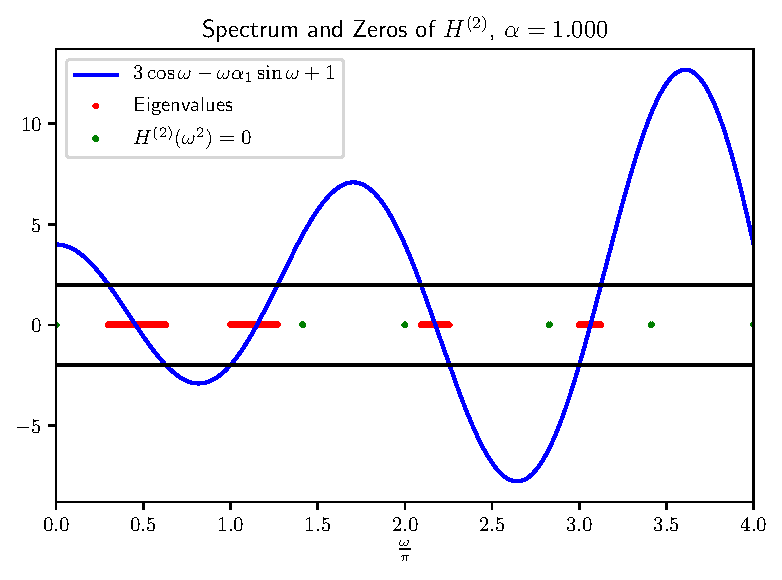
\includegraphics[scale=0.5]{1DDecoratedGraph_alpha1.pdf}
		\caption{\label{fig:1DDecoratedGraph_alpha1} The values of $\omega$ which solve \eqref{eq:EmbeddedGraphDetSolveCondition} with $\alpha_1=1$. No zeros of $H^{(2)}$ form part of the spectrum in this case.}
	\end{subfigure}
	~
	\begin{subfigure}[t]{0.45\textwidth}
		\centering
		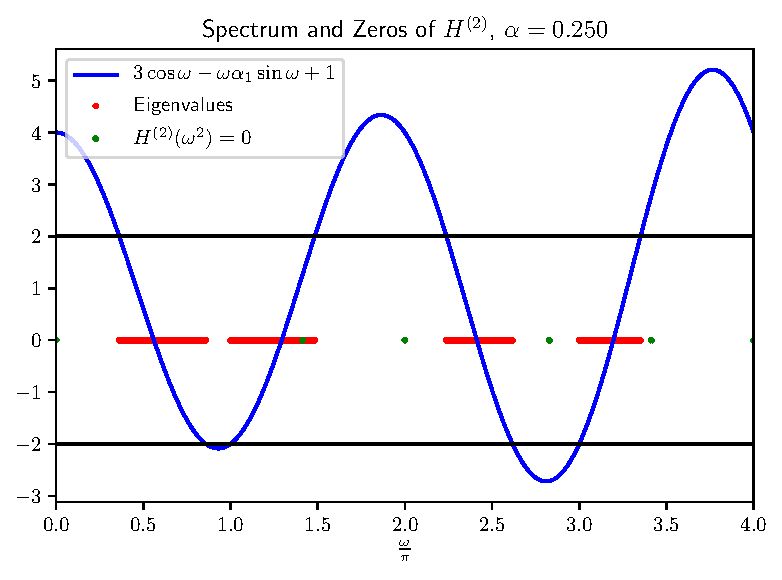
\includegraphics[scale=0.5]{1DDecoratedGraph_alpha0-25.pdf}
		\caption{\label{fig:1DDecoratedGraph_alpha0-25} The values of $\omega$ which solve \eqref{eq:EmbeddedGraphDetSolveCondition} with $\alpha_1=\recip{4}$. With $\alpha_1$ this small, some of the zeros of $H^{(2)}$ form part of the spectrum.}
	\end{subfigure}
	\caption{\label{fig:1DDecoratedGraph} The values of $\omega$ which solve \eqref{eq:EmbeddedGraphDetSolveCondition}, using $a=\recip{\sqrt{2}}$. Changing the value of $\alpha$ effects how many zeros of $H^{(2)}$ are included in the spectrum.}
\end{figure}
Zeros of $H^{(2)}$ occur at $\omega= 2n\pi, \frac{n\pi}{a}, \frac{n\pi}{b}$, which also solve \eqref{eq:EmbeddedGraphDetSolveCondition} for all values of $\qm$.
Examining the limit \eqref{eq:EigenvalueBranchLimit} reveals that if $H^{(2)}\bracs{\omega_0^2}=0$, $\omega_0$ is part of the spectrum only when there exists a $\qm_0\in\left[-\pi,\pi\right)$ such that $\Xi\bracs{\omega_0}=\cos\theta_0+\recip{2}$.
That is, the bracketed term in \eqref{eq:EmbeddedGraphDetSolveCondition} is required to be zero for a root of $H^{(2)}$ to be part of the spectrum.
The eigenvalue branches in the vicinity of root $\omega_0=\pi\sqrt{2}$ are plotted in figure \ref{fig:1DDecoratedGraphEvalBranches-Thetas}, to illustrate this point.
\begin{figure}[t!]
	\centering
	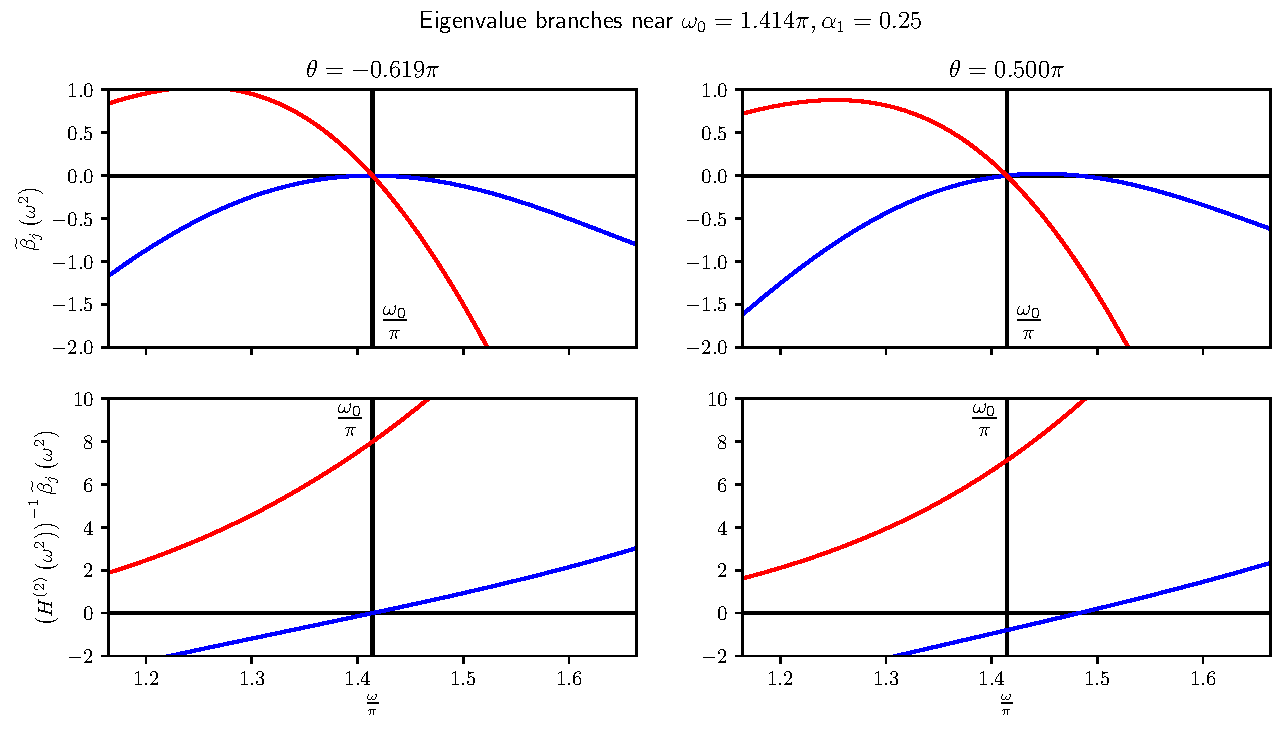
\includegraphics[scale=0.7]{1DDecoratedGraphEvalBranches-Thetas.pdf}
	\caption{\label{fig:1DDecoratedGraphEvalBranches-Thetas} eigenvalue branches of the matrix $\mathfrak{M}_{\qm}$ near $\omega_0 = \pi\sqrt{2}$, which is a root of $H^{(2)}$. The value $\qm_0\approx-0.691\pi$ solves $\Xi\bracs{\omega_0}=\cos\qm_0+\recip{2}$, and the limit \eqref{eq:EigenvalueBranchLimit} is zero. At other values of $\qm$ however, the limit \eqref{eq:EigenvalueBranchLimit} is non-zero.}
\end{figure}
It is also worth noting that (in figure \ref{fig:1DDecoratedGraphEvalBranches-Thetas}) there are two eigenvalue branches which are zero at $\omega_0$, with the third being non-zero at $\omega_0$.
For both branches, the limit \eqref{eq:EigenvalueBranchLimit} exists, however only for one is it zero.
The spectrum of \eqref{eq:SingularScalarWaveEqnWholeSpace} thus consists of those $\omega^2$ such that
\begin{align*}
	\abs{ 3\cos\omega - \alpha_1\omega\sin\omega + 1 } \leq 2.
\end{align*}
As expected, the spectrum does not depend on $\beta$ despite the fact that the $M$-matrix for each operator on $\graph_{\mathcal{P}}$ does.
It does differ from the spectrum of the quantum graph in section \ref{ssec:Example1DLoop} due to the presence of the ``decoration" $I_{12}$, although this difference only depends on the length this additional edge.

\subsection{Cross in the Periodic Plane} \label{ssec:ExampleCrossInPlane}
Our final example is a two-dimensional graph whose period cell represents a lattice-like structure in $\reals^2$.
Consider the embedded, periodic graph defined as follows --- for each $\bracs{n,m}\in\integers^2$ define
\begin{align*}
	v^{(n,m)} &= \bracs{n+\recip{2}, m+\recip{2}}, \quad
	I_{\mathrm{left}}^{\bracs{n,m}} = \sqbracs{v^{\bracs{n,m}}, v^{\bracs{n+1,m}}}, \quad
	I_{\mathrm{up}}^{\bracs{n,m}} = \sqbracs{v^{\bracs{n,m}}, v^{\bracs{n,m+1}}}, \\
	\vertSet^* &= \clbracs{v^{\bracs{n,m}} \setVert \bracs{n,m}\in\integers^2}, \quad
	\edgeSet^* = \clbracs{ I_{\mathrm{l}}^{\bracs{n,m}}, I_{\mathrm{u}}^{\bracs{n,m}} \setVert \bracs{n,m}\in\integers^2}, \quad
	\graph^* = \bracs{\vertSet^*, \edgeSet^*}.
\end{align*}
Place a coupling constant $\alpha^{\bracs{n,m}} =: \alpha_3>0$ at each $v^{(n,m)}$.
The period graph of $\graph^*$ occupies $\left[0,1\right)^2$ and consists of a single vertex with two looping edges of length 1.
Breaking the loops by introducing two artificial vertices takes us to the quantum graph
\begin{align*}
	\vertSet = \clbracs{v_1, v_2, v_3}, \quad
	\edgeSet = \clbracs{I_{13}, I_{31}, I_{23}, I_{32}}, \quad
	\graph = \bracs{\vertSet, \edgeSet},
\end{align*}
with
\begin{align*}
	l_{13} = b, \quad l_{31} = \tilde{b} := 1-b, \quad 
	l_{23} = a, \quad l_{32} = \tilde{a} := 1-a, \qquad
	\qm_{13} = \qm_{31} = \qm_2, \quad \qm_{23} = \qm_{32} = \qm_1,
\end{align*}
and coupling constant $\alpha_3$ at $v_3$ (and zero coupling constants at the dummy vertices $v_1$ and $v_2$).
Also define
\begin{align*}
	 s_a\bracs{\omega} = \sin\bracs{a\omega}, \quad 
	 c_a\bracs{\omega} = \cos\bracs{a\omega}, \quad 
	 s_b\bracs{\omega} = \sin\bracs{b\omega}, \quad 
	 c_b\bracs{\omega} = \cos\bracs{b\omega},
\end{align*}
\begin{align*}
	 \tilde{s}_a\bracs{\omega} = \sin\bracs{\omega\bracs{1-a}}, \quad 
	 \tilde{c}_a\bracs{\omega} = \cos\bracs{\omega\bracs{1-a}}, \quad 
	 \tilde{s}_b\bracs{\omega} = \sin\bracs{\omega\bracs{1-b}}, \quad 
	 \tilde{c}_b\bracs{\omega} = \cos\bracs{\omega\bracs{1-b}}.
\end{align*}
Using corollary \ref{cory:M-MatrixEntriesNoPoles} we set $H^{(2)}\bracs{\omega^2} = s_a\bracs{\omega} s_b\bracs{\omega} \tilde{s}_a\bracs{\omega} \tilde{s}_b\bracs{\omega}$, and obtain
\begin{align*}
	\mathfrak{M}_{\qm}\bracs{\omega^2} &=
	\begin{pmatrix}[2.5]
		-\omega s_a \tilde{s}_a \bracs{ s_b \tilde{c}_b + c_b \tilde{s}_b } &
		0 &
		\begin{split}
			&\omega s_a \tilde{s}_a \bracs{ e^{\rmi\qm_2\tilde{b}}s_b + e^{-\rmi\qm_2 b}\tilde{s}_b }
		\end{split} \\
		0 &
		-\omega s_b \tilde{s}_b \bracs{ s_a \tilde{c}_a + c_a \tilde{s}_a } &
		\begin{split}
			&\omega s_b \tilde{s}_b \bracs{ e^{\rmi\qm_1\tilde{a}}s_a + e^{-\rmi\qm_1 a}\tilde{s}_a } 
		\end{split} \\
		\omega s_a \tilde{s}_a \bracs{ e^{-\rmi\qm_2\tilde{b})}s_b + e^{\rmi\qm_2 b}\tilde{s}_b } &
		\omega s_b \tilde{s}_b \bracs{ e^{-\rmi\qm_1\tilde{a}}s_a + e^{\rmi\qm_1 a}\tilde{s}_a } &
		\begin{split}
			&-\omega ( s_a s_b \tilde{s}_a \tilde{c}_b 
			+ s_a s_b \tilde{c}_a \tilde{s}_b \\ 
			& + s_a c_b \tilde{s}_a \tilde{s}_b
			+ c_a s_b \tilde{s}_a \tilde{s}_b \\
			& - \omega\alpha_3 s_a s_b \tilde{s}_a \tilde{s}_b )
		\end{split}
	\end{pmatrix}.
\end{align*}
Examining \eqref{eq:QGDetSolveCondition} yields
\begin{align} \label{eq:ExampleThickVertexSolution}
	0 = \omega^3 s_a^2\bracs{\omega} s_b^2\bracs{\omega} \tilde{s}_a^2\bracs{\omega} \tilde{s}_b^2\bracs{\omega} \sin\bracs{\omega} 
	\bracs{ 4\cos\bracs{\frac{\qm_1+\qm_2}{2}}\cos\bracs{\frac{\qm_1-\qm_2}{2}} + \omega\alpha_3\sin\omega - 4\cos\omega}.
\end{align}
For ease, we define
\begin{align*}
	\Xi\bracs{\omega} := \cos\omega - \frac{\alpha_3\omega}{4}\sin\omega.
\end{align*}
From here, the analysis is similar to that of example \ref{ssec:EmbeddingDependentExample} --- any root of $H^{(2)}$ solves \eqref{eq:ExampleThickVertexSolution}, in addition to those $\omega$ for which $-1\leq\Xi\bracs{\omega}\leq 1$.
Examination of the eigenvalue branches then produces a familiar conclusion; if $H^{(2)}\bracs{\omega_0^2}=0$, $\omega_0$ forms part of the spectrum of \eqref{eq:SingularWaveEqnQGProblem} on $\graph$ if and only if there exists a $\qm_0$ such that the bracket in \eqref{eq:ExampleThickVertexSolution} is zero at $\bracs{\omega_0,\qm_0}$ -- that is if 
\begin{align} \label{eq:ExampleThickVertexSolutionReduced}
	\Xi\bracs{\omega}=\cos\bracs{\frac{\qm_1+\qm_2}{2}}\cos\bracs{\frac{\qm_1-\qm_2}{2}}.
\end{align}
As a result, the spectrum consists of exactly those $\omega$ such that
\begin{align*}
	-1 \leq \cos\omega - \frac{\alpha_3\omega}{4}\sin\omega \leq 1.
\end{align*}
In addition to recovering the spectrum of \eqref{eq:SingularWaveEqnQGProblem}, we can use \eqref{eq:ExampleThickVertexSolution} and \eqref{eq:QGGenEvalSolveNoPoles} to recover the eigenfunctions too.
For a given $\qm$, equation \eqref{eq:ExampleThickVertexSolutionReduced} can be solved for (a solution) $\omega=\omega_0$.
This $\omega_0$ corresponds to an eigenvalue $\omega_0^2$ of \eqref{eq:SingularWaveEqnQGProblem}, but also implies that there exists a $w\in\complex^{\abs{\vertSet}}$ such that \eqref{eq:QGGenEvalSolveNoPoles} holds at $\omega=\omega_0$.
Given that we can compute $\mathfrak{M}_{\qm}\bracs{\omega_0^2}$, and we \emph{know} $\mathfrak{M}_{\qm}\bracs{\omega_0^2}$ has a zero eigenvalue, it is not hard to (numerically) determine the associated eigenvector(s) $w$.
By definition of $\mathfrak{M}_\qm$ and the $M$-matrix, this vector $w = \dmap u$ is the Dirichlet data of the eigenfunction $u$ that corresponds to the eigenvalue $\omega_0^2$.
Given \eqref{eq:EdgeEqnGeneralSolution} and $w$, it is thus possible to reconstruct each of the edge functions $u^{(jk)}$ --- some examples of the result of this process are plotted in figure \ref{fig:CrossInPlane-EdgePlot}.
\begin{figure}[h!]
	\begin{subfigure}[t]{0.45\textwidth}
		\centering
		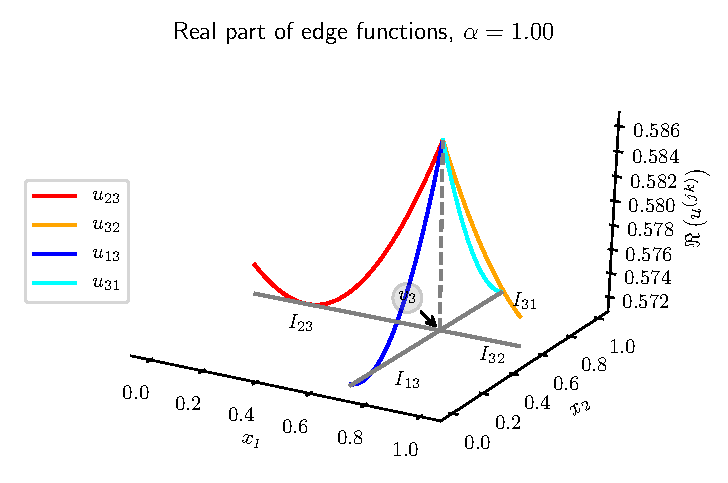
\includegraphics[scale=0.6]{CrossInPlane_EdgePlot-R-a1.pdf}
		\caption{\label{fig:CrossInPlane_EdgePlot-R-a1} The real part of the eigenfunction when $\omega_0=0.63936, \alpha=1$.}
	\end{subfigure}
	~
	\begin{subfigure}[t]{0.45\textwidth}
		\centering
		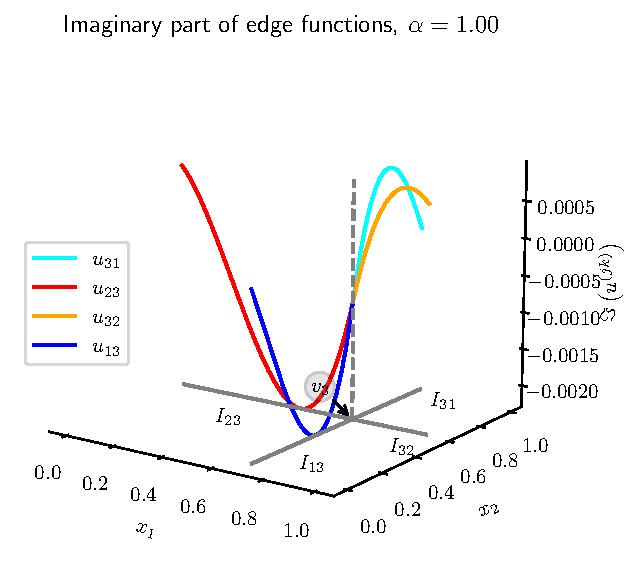
\includegraphics[scale=0.6]{CrossInPlane_EdgePlot-I-a1.pdf}
		\caption{\label{fig:CrossInPlane_EdgePlot-I-a1} The imaginary part of the eigenfunction when $\omega_0=0.63936, \alpha=1$.}
	\end{subfigure}
	\vskip\baselineskip
	\begin{subfigure}[t]{0.45\textwidth}
		\centering
		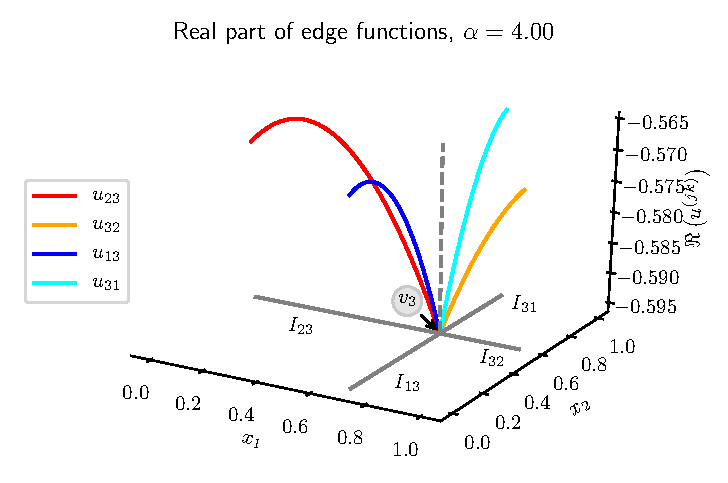
\includegraphics[scale=0.6]{CrossInPlane_EdgePlot-R-a4.pdf}
		\caption{\label{fig:CrossInPlane_EdgePlot-R-a4} The real part of the eigenfunction when $\omega_0=0.44812, \alpha=4$.}
	\end{subfigure}
	~
	\begin{subfigure}[t]{0.45\textwidth}
		\centering
		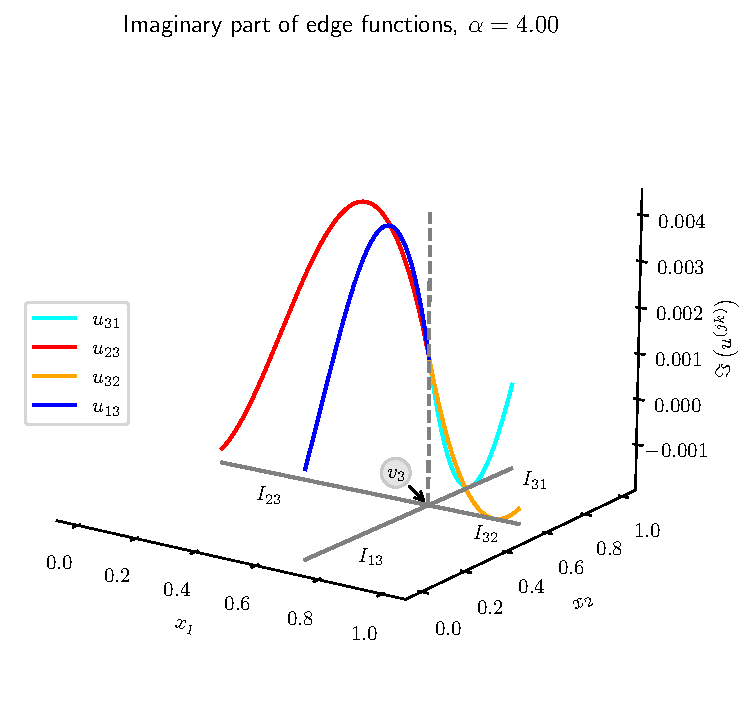
\includegraphics[scale=0.6]{CrossInPlane_EdgePlot-I-a4.pdf}
		\caption{\label{fig:CrossInPlane_EdgePlot-I-a4} The imaginary part of the eigenfunction when $\omega_0=0.44812, \alpha=4$.}
	\end{subfigure}	
	\caption{\label{fig:CrossInPlane-EdgePlot} Plots of the eigenfunction corresponding to the eigenvalue $\omega_0=0.63936$  when $\alpha=1$, and $\omega_0=0.44812$ when $\alpha=4$. Both eigenvalues are attained when $\qm=\bracs{\frac{\pi}{4},\frac{\pi}{4}}^\top$, and the edge functions are plotted above the graph $\graph$ in the $\bracs{x_1,x_2}$-plane.}
\end{figure}

To round off the analysis, quantities such as the integrated density of states (IDoS) and density of states (DoS) can also be estimated from \eqref{eq:ExampleThickVertexSolution}, shown in figure \ref{fig:CrossInPlane_ScalarDoS}, displaying the band-gap structure of the spectrum and demonstrating that the eigenvalues ``concentrate" at the center of each spectral band.
\begin{figure}[t!]
	\begin{subfigure}[t]{0.45\textwidth}
		\centering
		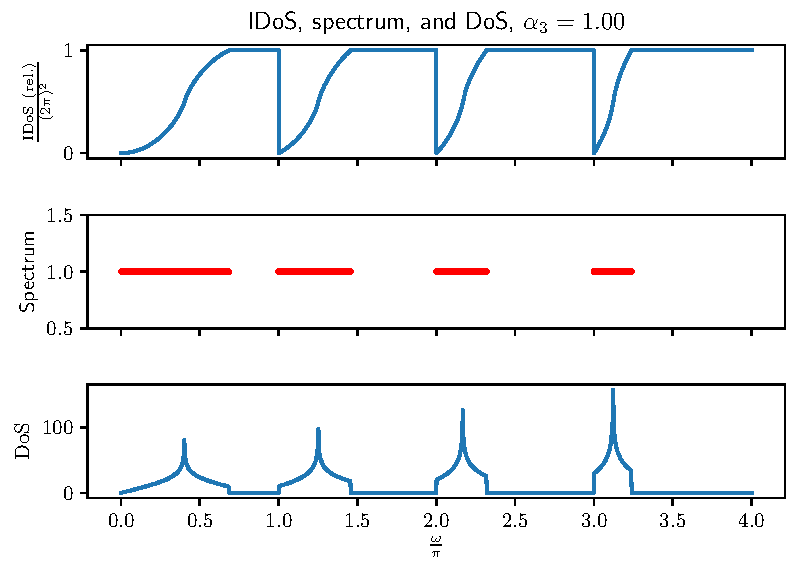
\includegraphics[scale=0.5]{CrossInPlane_ScalarDoS_alpha1-00.pdf}
		\caption{\label{fig:CrossInPlane_ScalarDoS_alpha1-00} The (relative) integrated density of states (IDoS), density of states (DoS) and spectrum for the system with $\alpha_3=1$.}
	\end{subfigure}
	~
	\begin{subfigure}[t]{0.45\textwidth}
		\centering
		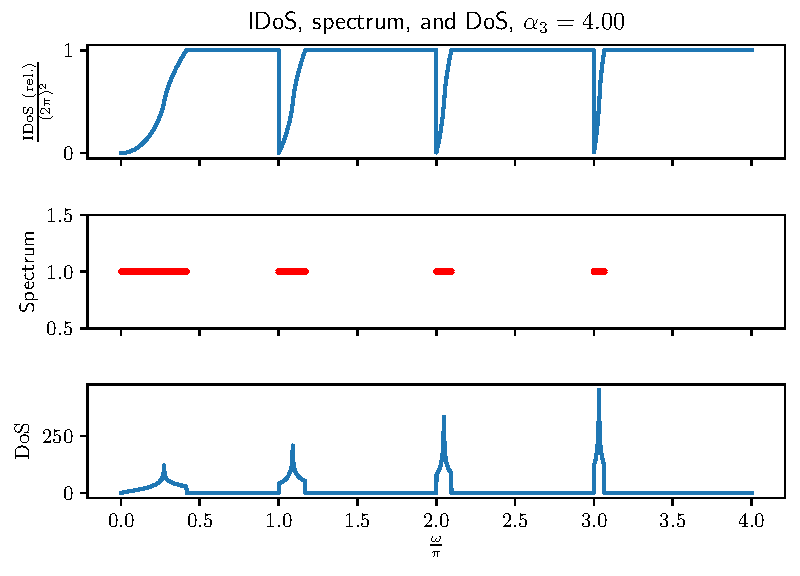
\includegraphics[scale=0.5]{CrossInPlane_ScalarDoS_alpha4-00.pdf}
		\caption{\label{fig:CrossInPlane_ScalarDoS_alpha4-00} The (relative) integrated density of states (IDoS), density of states (DoS) and spectrum for the system with $\alpha_3=4$.}
	\end{subfigure}	
	\caption{\label{fig:CrossInPlane_ScalarDoS} The (relative) IDoS, DoS, and spectrum for the graph topology in section \ref{ssec:ExampleCrossInPlane}.
	The relative IDoS at the value $x$ is defined as the IDoS at the value $x$ minus $\left\lfloor\frac{x}{\pi}\right\rfloor\bracs{2\pi}^2$.}
\end{figure}
For any $\alpha_3>0$, it can also be shown that the spectral bands $I_n$ satisfy $I_n\subset\sqbracs{(n-1)\pi, n\pi}$, each with left-endpoint $(n-1)\pi$ and a right-endpoint strictly less than $n\pi$.
It is worth remarking that this behaviour is reversed for $\alpha_3<0$, the bands having right-endpoint $n\pi$ and left-endpoint strictly greater than $(n-1)\pi$.
For $\alpha\leq-2$ there is even a gap between an isolated eigenvalue at $0$ and the beginning of the band $I_1$ --- however as mentioned in section \ref{sec:ScalarEqnChapterIntro}, $\alpha<0$ does not correspond to any physical material.
This result is consistent with similar applications of singular-structures as approximations to thin-material structures, like the work of \cite{cherednichenko2019time}, in which the natural physical constraints on the parameters in the problem prevent a similar opening of a band-gap at the bottom of the spectrum.


%Curl-curl equation plus 1st order Maxwell chapter begins
\chapter{Curl-of-the-Curl Equation} \label{ch:CurlCurl}
\tstk{make this title more focused when the time comes.}

%\input{./Chapters/Curl-Curl/Introduction}

\subsection{Geometric Interpretation of Tangential Curls} \label{ssec:CC-Geometric}
Unlike the gradient, the curl of a vector field does not have an intuitive one-dimensional analogue that we can appeal to when looking to work on singular structure domains.
This makes the analysis of section \ref{sec:CC-CurlAnalysis} crucial to our understanding of the curl of the curl equation \tstk{ref!}.
In the interests of providing the reader an intuitive idea of what the tangential curl is for a singular measure, we provide a geometric interpretation in this section prior to beginning the process of deriving a quantum graph problem from our variational formulation.
We will also address a remark made in section \ref{sec:TP-DomainSetup}, concerning why we do not consider a singular structure modelled by a (periodic) graph embedded into $\reals^3$, and instead consider a domain formed from the extrusion into 3 dimensions of a periodic graph embedded in $\reals^2$.

Let us begin by demonstrating why curls of zero on a singular structure embedded into $\reals^3$ do not give rise to any interesting variational problems.
Consider a segment $I_{jk}\subset\reals^3$, with $I_{jk} = \clbracs{0}\times\sqbracs{0,l_{jk}}\times\clbracs{0}$, which we can view as one edge of a graph embedded into $\reals^3$.
We can then prove the following result:
\begin{prop} \label{prop:3DGraph-CurlsAreZero}
	Every vector field is a curl of zero, that is
	\begin{align*}
		\curlZero{\reals^3}{\lambda_{jk}} = \ltwo{\reals^3}{\lambda_{jk}}^3,
	\end{align*}
	and consequentially every vector field $u\in\ltwo{\reals^3}{\lambda_{jk}}^3$ is also an element of $\ktcurlSob{\reals^3}{\lambda_{jk}}$ with tangential curl equal to zero.
\end{prop}
The assumption on the position and orientation of $I_{jk}$ is not restrictive, in the sense that the result we prove will generalise to any line segment (and thus edge) in $\reals^3$.
This result also holds when we replace $\reals^3$ with a finite domain $U\subset\reals^3$ (with non-zero $\lambda_3$-measure) and consider $I_{jk}\subset U$, and consequentially if we consider $U$ the period cell of some 3-dimensional singular structure $\graph$ and consider curls on the torus.
\begin{proof}
	We construct explicit approximating sequences for any function in $\ltwo{\reals^3}{\lambda_{jk}}^3$, by first considering $\phi\in\smooth{\reals^3}$.
	Consider the vector field $\varphi^{(2)} = -x_1\phi\widehat{x}_3\in\smooth{\reals^3}^3$ --- note that we can always multiply $\varphi^{(2)}$ by a smooth cut-off function which is equal to unity on $I_{jk}$ to obtain a compactly supported smooth function if we are so inclined.
	Then we can observe that $\varphi^{(2)}=0$ on $I_{jk}$ (since $x_1=0$ here) and 
	\begin{align*}
		\curl{}\varphi^{(2)} = -x_1\partial_2\phi\widehat{x}_1 + \bracs{\phi + x_1\partial_1\phi}\widehat{x}_2,
	\end{align*}
	which is equal to $\phi\widehat{x}_2$ on $I_{jk}$.
	This implies that $\varphi^{(2)}$ serves as an approximating ``sequence" with
	\begin{align*}
		\varphi^{(2)} \lconv{\ltwo{\reals^3}{\lambda_{jk}}^3} 0, 
		\qquad
		\curl{}\varphi^{(2)} \lconv{\ltwo{\reals^3}{\lambda_{jk}}^3} \phi\widehat{x}_2,
	\end{align*}
	so $\phi\widehat{x}_2\in\curlZero{\reals^3}{\lambda_{jk}}$.
	Consideration of the functions $\varphi^{(1)} = -x_3\phi\widehat{x}_2$ and $\varphi^{(3)}=x_1\phi\widehat{x}_2$ demonstrates that $\phi\widehat{x}_1$ and $\phi\widehat{x}_3$ are also elements of $\curlZero{\reals^3}{\lambda_{jk}}$.
	By linearity, we have that $\smooth{\reals^3}^3\subset\curlZero{\reals^3}{\lambda_{jk}}$ and then by the density of smooth functions in $\ltwo{\reals^3}{\lambda_{jk}}$, we obtain
	\begin{align*}
		\curlZero{\reals^3}{\lambda_{jk}} = \ltwo{\reals^3}{\lambda_{jk}}^3.
	\end{align*}
	We can also infer that any smooth vector field $\Phi\in\smooth{\reals^3}{\lambda_{jk}}^3$ is an element of $\ktcurlSob{\reals^3}{\lambda_{jk}}$ with $\ktcurl{\lambda_{jk}}\Phi = 0$ since $\ltwo{\reals^3}{\lambda_{jk}}^{\perp} = \clbracs{0}$.
	Density of smooth functions in $\ltwo{\reals^3}{\lambda_{jk}}^3$ then demonstrates that any $u\in\ltwo{\reals^3}{\lambda_{jk}}^3$ is also an element of $\ktcurlSob{\reals^3}{\lambda_{jk}}$ with tangential curl equal to zero.
\end{proof}
That is to say, a singular structure in 3 dimensions represented by a graph does not give rise to any non-trivial notion of the curl of a vector field.
Needless to say, this makes exploration of the curl of the curl equation trivial in this context --- it is clear from section \ref{sec:CC-CurlAnalysis} that tangential curls with respect to the measure $\ddmes$ will inherit the behaviour of tangential curls with respect to each $I_{jk}$ on the respective edges, and thus only produce trivial variational problems.

Rather than examining a graph embedded into $\reals^3$, let us instead return to the domain $\dddom$.
First, recall that $\dddom$ consists of a periodic graph embedded into $\reals^2$ with unit cell $\ddom$, and then extruded into $\dddom = \ddom\times[0,\infty)$ to form a domain that consists of a union of planes parallel to the $x_3$-axis.
Our use of a Fourier transform in $x_3$ then brings us back onto the 2 dimensional domain $\ddom$, however it is important for us to remember that each edge of $\graph$ in $\ddom$ actually represents a \emph{plane} in $\reals^3$.
In what follows, we will let $P_{jk}$ be the plane induced by the edge $I_{jk}$ of the graph $\graph$, so $P_{jk} = I_{jk}\times[0,\infty)\subset\ddom\times[0,\infty)$.

Classically, one can interpret the curl $c$ of a vector field $u$ by identifying $c(x)$ as the axis of rotation that an (infinitesimally small) spherical body would undergo if placed in the field $u$ at position $x$, with the angular speed of the rotation equal to half the magnitude of $c(x)$.
Our intuition and geometric interpretation for tangential gradients (section \ref{ssec:3DGradGeometric}) was largely based on the idea that the singular measure $\lambda_{jk}$ cannot ``see" changes in functions \emph{across} the edges $I_{jk}$.
Formally, the interpretation we have for tangential curls (and curls of zero) also appeals to this idea; the measure $\lambda_{jk}$ does not have any concept of normal derivative across $I_{jk}$, and correspondingly the product measure $\lambda_{jk}\times\lambda_1$ does not have any concept of a derivative \emph{outward} from the plane $P_{jk}$.
However, when we are restricted to only observing the values of $u$ in the plane $P_{jk}$, any changes in $u$ in the direction of the outward normal $\widehat{n}_{jk}$ to $P_{jk}$ cannot be seen, or observed.
Such changes in $u$ only affect the components of $c(x)$ in the directions orthogonal to $\widehat{n}_{jk}$, but if we do not know how we are rotating in one direction, we do not know how to orient \emph{the axis} about which we rotate.
In this case, the directions $\widehat{e}_{jk}$ and $\widehat{x}_3$ are those which are orthogonal to $\widehat{n}_{jk}$ (corollary \ref{cory:CurlZero-Rotated}).
On the other hand, the only component of $c(x)$ that isn't derived from changes in $u$ in the direction $\widehat{n}_{jk}$ is the component along the direction $\widehat{n}_{jk}$ itself, which is the only component in tangential curls that is non-zero (corollary \ref{cory:TangCurlEdgeRotated}).
This idea carries over into our previous consideration of singular structures (and conclusion in proposition \ref{prop:3DGraph-CurlsAreZero}) in three dimensions too ---  $\lambda_{jk}$ still has no concept of derivative across the edge $I_{jk}$, and in three dimensions this means there are two linearly independent directions in which rates of change cannot be seen.
Consequentially, we can never accurately reconstruct the axis about which we are rotating, as all three components of the curl would need to know the rate of change in $u$ in at least one of the directions normal to $I_{jk}$.
The measure $\massMes$ tells a similar story --- except in this case we have thrown away the ability to detect change in \emph{every} axial direction!

For a visual interpretation of tangential curls, one can imagine the following picture (illustrated in figure \ref{fig:Diagram_CurlGeometric} with the commentary that follows).
Place a sphere of radius $\ll 1$\footnote{Or alternatively, think of the sphere as being infinitesimally small.} centred at a point $x\in P_{jk}$.
Place a point $p$ on the intersection between the surface of the sphere and the plane $P_{jk}$, and consider the (closed) path $\gamma_p$ that $p$ traces out under the rotation induced by the vector field $u$.
Under the axis of rotation provided by $\ktcurl{\lambda_{jk}}u$, the curve $\gamma_p$ will be entirely contained in the plane $P_{jk}$, and thus the rotation is ``visible" to\footnote{Or for want of a better phrase, the rotation \emph{traces out a path that can be followed by}.} the measure $\lambda_{jk}\times\lambda_1$.
\begin{figure}[b!]
	\centering
	\includegraphics[scale=1.0]{./Diagram_CurlGeometric.pdf}
	\caption{\label{fig:Diagram_CurlGeometric} An illustration of the notation of tangential curl and curls of zero on $P_{jk}$. Tangential curls cause points on an (infinitesimally small) sphere to rotate within the plane $P_{jk}$, whilst curls of zero induce rotations that move points on the sphere out of the plane.}
\end{figure}
However under the axis of rotation provided by a curl of zero, the curve $\gamma_p$ is not contained in the plane $P_{jk}$ --- in fact, it's intersection with the plane will be at most a finite number of points.
If instead $P_{jk}\cap\gamma_p\supset\clbracs{p,p^*}$ for $p^*\neq p$, the measure $\lambda_{jk}\times\lambda_1$ still has no way of knowing \emph{how} $p$ travelled to $p^*$, since the path $\gamma_p$ is not visible (and, from the 3-dimensional perspective, there are infinitely many curls of varying magnitudes that could rotate $p$ to $p^*$ and back).
In the event that $P_{jk}\cap\gamma_p=\clbracs{p}$, then it appears that the sphere is not rotating at all.
That is to say, curls of zero induce rotations ``out of the plane" $P_{jk}$, which the measure $\lambda_{jk}$ cannot observe, whilst tangential curls ensure that all rotation happens ``within" the plane $P_{jk}$.

\tstk{now it's time for the summary of key tangential curl results.}
Similarly to chapter \ref{ch:ScalarSystem}, having an edge-wise behaviour for the tangential curl and curls of zero (that is, with respect to $\lambda_{jk}$) will allow us to construct those with respect to $\ddmes$ and $\dddmes$.
These arguments are the focus of section \ref{sec:CC-CurlAnalysis}, however we again provide the reader with a summary of the key properties of the tangential curl so that the manipulations in section \tstk{derivation section} can be followed, and to provide some familiarity with the objects that are discussed in \tstk{discussion session where everything is broken}.
To this end, a function $u\in\ktcurlSob{\ddom}{\dddmes}$ has the following properties:
\begin{enumerate}[(i)]
	\item On a given edge $I_{jk}$, we have that $\ktcurl{\dddmes}u = \ktcurl{\lambda_{jk}}u$.
	\item Along the edge $I_{jk}$, only the ``in-plane" components of $u$ are relevant.
	To this end we set $U^{(jk)} = R_{jk}\begin{pmatrix} u^{(jk)}_1 \\ u^{(jk)}_2 \end{pmatrix}$.
	Then we have that $\ktcurl{\lambda_{jk}}u = \bracs{u_3' + \rmi\qm_{jk}u_3 - \rmi\wavenumber U^{(jk)}_2}\widehat{n}_{jk}$, where $\qm_{jk}$ are the same constants from section \ref{sec:ScalarDerivation}, and $u_3'$ is the derivative in the $H^1$ sense of $u^{(jk)}_3\circ r_{jk}$.
	The term $\rmi\wavenumber U^{(jk)}_2$ resembles the information about any rotation induced by changes in $u$ along the $x_3$-axis that the measure $\lambda_{jk}\times\lambda_1$ can see.
	\item We have that $u_3\in\ktgradSob{\ddom}{\dddmes}$, so in particular it is continuous at each vertex $v_j$.
	\item At each $v_j$, we have that $\ktcurl{\dddmes}u = 0$.
\end{enumerate}
\tstk{why did we bother with divergence free stuff, maybe this should come after we get back to the scalar system post-derivation...}

%\section{Reduction to a Quantum Graph Problem} \label{sec:3DSystemDerivation}
We now look to find an alternative formulation of \eqref{eq:SingularCurlEquation}, which is more amenable to analysis.
Similarly to our working in section \ref{sec:ScalarDerivation}, the result will be a problem realisable as a quantum graph problem.
To ease the notational burden, for $u=\bracs{u_1,u_2,u_3}^\top\in\ktcurlSob{\ddom}{\dddmes}$ and $\Phi=\bracs{\phi_1,\phi_2,\phi_3}^\top\in\psmooth{\ddom}^3$ we define (for each $I_{jk}\in\edgeSet$),
\begin{align*}
	U^{(jk)} := R_{jk} \begin{pmatrix} u_1^{(jk)} \\ u_2^{(jk)} \end{pmatrix},
	\qquad
	\Psi^{(jk)} := R_{jk} \begin{pmatrix} \phi_1^{(jk)} \\ \phi_2^{(jk)} \end{pmatrix}.
\end{align*}
We use an overhead tilde to denote composition with $r_{jk}$, and for a function $v$ with $\widetilde{v}^{(jk)}\in\ktgradSob{\sqbracs{0,l_{jk}}}{y}$ write $\bracs{v^{(jk)}}' := \bracs{\widetilde{v}^{(jk)}}' \circ r_{jk}^{-1}$.
Finally, for a given quasi-momentum $\qm$ we set $\qm_{jk} = \qm\cdot e_{jk}$.

Now suppose that $u\in\ktcurlSob{\ddom}{\dddmes}$ is divergence free with respect to $\dddmes$, and is a solution to \eqref{eq:SingularCurlEquation} for some $\omega>0$, and take arbitrary $\varphi_1,\varphi_2\in\csmooth{\sqbracs{0,l_{jk}}}$.
Since $R_{jk}\in\mathrm{SO}(2)$, the system
\begin{align*}
	\begin{pmatrix} \phi_1 \\ \phi_2 \end{pmatrix} &= R_{jk}^\top \begin{pmatrix} \varphi_1 \\ \varphi_2 \end{pmatrix}
\end{align*}
has a unique solution for $\bracs{\phi_1,\phi_2}^\top$, and we can construct a $\Phi\in\csmooth{\ddom}$ with $\supp\Phi\cap\graph\subset I_{jk}^{\circ}$, $\widetilde{\Psi}_1^{(jk)}=\varphi_1$, and $\widetilde{\Psi}_2^{(jk)}=\varphi_2$.
Fix an edge $I_{jk}$ and take $\Phi$ such that $\supp\Phi\cap\graph\subset I_{jk}^{\circ}$.
The equation \eqref{eq:SingularCurlEquation-VariationalForm} reduces to
\begin{align*}
	\omega^2 \integral{I_{jk}}{ u\cdot\overline{\Phi} }{\lambda_{jk}}
	&= \integral{I_{jk}}{ \ktcurl{\ddmes}u\cdot\overline{\ktcurl{\ddmes}\Phi} }{\lambda_{jk}} \\
	&= \integral{I_{jk}}{ \bracs{ \bracs{u_3^{(jk)}}' + \rmi\qm_{jk} u_3^{(jk)} - \rmi\wavenumber U_2^{(jk)} }\overline{\bracs{ \bracs{\phi_3^{(jk)}}' + \rmi\qm_{jk} \phi_3^{(jk)} - \rmi\wavenumber \Psi_2^{(jk)} }} }{\lambda_{jk}}.
\end{align*}
Using the change of variables $r_{jk}$ we obtain
%\begin{align*}
%	\int_0^{l_{jk}} & \bracs{ \bracs{\widetilde{u}_3^{(jk)}}' + \rmi\qm_{jk} \widetilde{u}_3^{(jk)} - \rmi\wavenumber \widetilde{U}_2^{(jk)} } \bracs{ \bracs{\overline{\widetilde{\phi}}_3^{(jk)}}' - \rmi\qm_{jk} \overline{\widetilde{\phi}}_3^{(jk)} + \rmi\wavenumber \overline{\widetilde{\Psi}}_2^{(jk)} } \ \md y \\
%	&= \omega^2 \int_0^{l_{jk}} \widetilde{U}_1^{(jk)}\overline{\widetilde{\Psi}}_1^{(jk)} + \widetilde{U}_2^{(jk)}\overline{\widetilde{\Psi}}_2^{(jk)} + \widetilde{u}_3^{(jk)}\overline{\widetilde{\phi}}_3^{(jk)} \ \md y.
%\end{align*}
%We thus observe that
\begin{align*}
	\int_0^{l_{jk}} & \bracs{ \bracs{\widetilde{u}_3^{(jk)}}' + \rmi\qm_{jk} \widetilde{u}_3^{(jk)} - \rmi\wavenumber \widetilde{U}_2^{(jk)} } \bracs{ \bracs{\overline{\widetilde{\phi}}_3^{(jk)}}' - \rmi\qm_{jk} \overline{\widetilde{\phi}}_3^{(jk)} + \rmi\wavenumber \overline{\varphi_2} } \ \md y \\
	&= \omega^2 \int_0^{l_{jk}} \widetilde{U}_1^{(jk)}\overline{\varphi_1} + \widetilde{U}_2^{(jk)}\overline{\varphi_2} + \widetilde{u}_3^{(jk)}\overline{\widetilde{\phi}}_3^{(jk)} \ \md y,
\end{align*}
which holds for any $\varphi_1,\varphi_2,\widetilde{\phi}_3^{(jk)}\in\csmooth{\sqbracs{0,l_{jk}}}$.
Therefore it must hold that for any $\varphi\in\csmooth{\sqbracs{0,l_{jk}}}$,
\begin{subequations}
	\begin{align*}
		0 &= \int_0^{l_{jk}} \overline{\varphi} \widetilde{U}_1^{(jk)} \ \md y, \labelthis\label{eq:CurlCurlWeakFormPhi1} \\
		0 &= \int_0^{l_{jk}} \overline{\varphi} \bracs{ \rmi\wavenumber\bracs{\widetilde{u}_3^{(jk)}}' + \bracs{\wavenumber^2 - \omega^2}\widetilde{U}_2^{(jk)} - \wavenumber\qm_{jk}\widetilde{u}_3^{(jk)}  } \ \md y, \labelthis\label{eq:CurlCurlWeakFormPhi2} \\
		0 &= \int_0^{l_{jk}} \overline{\varphi}' \bracs{ \bracs{\widetilde{u}_3^{(jk)}}'
		- \rmi\wavenumber\widetilde{U}_2^{(jk)} + \rmi\qm_{jk}\widetilde{u}_3^{(jk)} } \\
		&\qquad -\rmi\qm_{jk}\overline{\varphi}\bracs{ \bracs{\widetilde{u}_3^{(jk)}}' - \rmi\wavenumber\widetilde{U}_2^{(jk)} + \rmi\qm_{jk}\widetilde{u}_3^{(jk)} }
		- \omega^2 \widetilde{u}_3^{(jk)}\overline{\varphi} \ \md y. \labelthis\label{eq:CurlCurlWeakFormPhi3}
	\end{align*}
\end{subequations}
The equation \eqref{eq:CurlCurlWeakFormPhi1} implies that $U_1^{(jk)}=0$ on $I_{jk}$, whilst \eqref{eq:CurlCurlWeakFormPhi2} implies that
\begin{align*}
	\rmi\wavenumber\bracs{\diff{}{y} + \rmi\qm_{jk}}\widetilde{u}_3^{(jk)} + \wavenumber^2\widetilde{U}_2^{(jk)} &= \omega^2\widetilde{U}_2^{(jk)},
\end{align*}
on $I_{jk}$.
Given that $u$ is divergence-free, proposition \ref{prop:DivFree-AllGradsConditions} informs us that $\widetilde{U}_2^{(jk)}$ is weakly differentiable in the $\gradSob{\sqbracs{0,l_{jk}}}{y}$-sense and we can manipulate \eqref{eq:CurlCurlWeakFormPhi3} to obtain
\begin{align*}
	\int_0^{l_{jk}} \overline{\varphi}' \widetilde{u}'_{3,jk} \ \md y
	&= -\int_0^{l_{jk}} \overline{\varphi} \bracs{ \rmi\wavenumber\widetilde{U}'_{2,jk} - \wavenumber\qm_{jk}\widetilde{U}_{2,jk} - 2\rmi\qm_{jk}\widetilde{u}'_{3,jk} + \qm_{jk}^2\widetilde{u}_{3,jk} - \omega^2\widetilde{u}_{3,jk} } \ \md y.,
\end{align*}
for all $\varphi\in\csmooth{\sqbracs{0,l_{jk}}}$.
Thus we can conclude that $\widetilde{u}_3\in\gradgradSob{\sqbracs{0,l_{jk}}}{y}$, from which we deduce that
\begin{align*}
	-\bracs{ \diff{}{y} + \rmi\qm_{jk} }^2\widetilde{u}_3^{(jk)} + \rmi\wavenumber\bracs{ \diff{}{y} + \rmi\qm_{jk} }\widetilde{U}_2^{(jk)} &= \omega^2 \widetilde{u}_3^{(jk)}
\end{align*}
on $I_{jk}$.
This provides us with a system of two coupled ODEs on each of the edges $I_{jk}$.
The information that the component $\widetilde{U}_1^{(jk)}=0$ on each edge is also obtained, which we remark is one of the consequences of $u$ being divergence-free with respect to $\dddmes$.

Now we look at how these edge ODEs are coupled at the vertices.
Fix a vertex $v_j$ and consider a $\Phi\in\csmooth{\ddom}$ whose support contains $v_j$ in its interior, and no other vertices of $\graph$.
Testing against such $\Phi$ in \eqref{eq:SingularCurlEquation-VariationalForm} implies that
\begin{align*}
	\alpha_j\omega^2 u(v_j)\cdot\overline{\Phi}(v_j)
	&= \integral{\ddom}{ \ktcurl{\ddmes}u\cdot\overline{\ktcurl{\ddmes}\Phi} - \omega^2 u\cdot\overline{\Phi} }{\ddmes} \\
	&= \sum_{j\con k}\integral{I_{jk}}{ \bracs{ \bracs{u_3^{(jk)}}' + \rmi\qm_{jk}u_3^{(jk)} - \rmi\wavenumber U_2^{(jk)}} \bracs{ \bracs{\overline{\phi}_3^{(jk)}}' - \rmi\qm_{jk}\overline{\phi}_3^{(jk)} + \rmi\wavenumber \overline{\Psi}_2^{(jk)}} \\
	&\qquad - \omega^2 U_1^{(jk)}\overline{\Psi}_1 - \omega^2 U_2^{(jk)}\overline{\Psi}_2 - \omega^2 u_3^{(jk)}\overline{\phi}_3 }{\lambda_{jk}} \\
	&= \sum_{j\con k}\int_0^{l_{jk}} \bracs{ \bracs{\widetilde{u}_3^{(jk)}}' + \rmi\qm_{jk}\widetilde{u}_3^{(jk)} - \rmi\wavenumber \widetilde{U}_2^{(jk)}} \bracs{ \bracs{\overline{\widetilde{\phi}}_3^{(jk)}}' - \rmi\qm_{jk}\overline{\widetilde{\phi}}_3^{(jk)} + \rmi\wavenumber \overline{\widetilde{\Psi}}_2^{(jk)}} \\
	&\qquad - \bracs{\bracs{\widetilde{u}_3^{(jk)}}' + \rmi\qm_{jk}\widetilde{u}_3^{(jk)} - \rmi\wavenumber \widetilde{U}_2^{(jk)}}\rmi\wavenumber\overline{\widetilde{\Psi}_2^{(jk)}} - \omega^2 \widetilde{u}_3^{(jk)}\overline{\widetilde{\phi}}_3 \ \md y \\
	&= -\sum_{j\con k}\int_0^{l_{jk}} \overline{\widetilde{\phi}}_3
	\sqbracs{ \bracs{\widetilde{u}_3^{(jk)}}'' + 2\rmi\qm_{jk}\bracs{\widetilde{u}_3^{(jk)}}' + \bracs{\rmi\qm_{jk}}^2\widetilde{u}_3^{(jk)} + \omega^2\widetilde{u}_3^{(jk)} } \\
	&\qquad - \overline{\widetilde{\phi}}_3\sqbracs{\rmi\wavenumber\bracs{ \bracs{\widetilde{U}_2^{(jk)}}' + \rmi\qm_{jk}\widetilde{U}_2^{(jk)} } } \ \md y \\
	&\qquad + \overline{\phi}_3(v_j)\sqbracs{ \sum_{j\con k}\bracs{\pdiff{}{n}+\rmi\qm_{jk}}u_3^{(jk)}(v_j) + \sum_{j\conRight k}U_2^{(kj)}(v_j) - \sum_{j\conLeft k}U_2^{(jk)}(v_j) } \\
	&= \overline{\phi}_3(v_j)\sqbracs{ \sum_{j\con k}\bracs{\pdiff{}{n}+\rmi\qm_{jk}}u_3^{(jk)}(v_j) + \sum_{j\conRight k}U_2^{(kj)}(v_j) - \sum_{j\conLeft k}U_2^{(jk)}(v_j) },
\end{align*}
where $U_2^{(jk)}(v_j)$ is the trace of $U_2^{(jk)}$ to the vertex $v_j$ --- these exist since $\widetilde{U}_2^{(jk)}(v_j)\in\gradSob{\sqbracs{0,l_{jk}}}{y}$, although of course they do not have to coincide at common vertices.
Identifying that the above procedure can be conducted for any $\phi_1(v_j), \phi_2(v_j), \phi_3(v_j)\in\complex$, we conclude that
\begin{align*}
	u_1(v_j) &= 0, \\
	u_2(v_j) &= 0, \\
	\alpha_j\omega^2u_3(v_j) &= \sum_{j\con k}\bracs{\pdiff{}{n}+\rmi\qm_{jk}}u_3^{(jk)}(v_j) + \sum_{j\conRight k}U_2^{(kj)}(v_j) - \sum_{j\conLeft k}U_2^{(jk)}(v_j).
\end{align*}

We are thus presented with the following set of equations on each edge $I_{jk}$;
\begin{subequations} \label{eq:QGRawSystem}
	\begin{align}
		\widetilde{U}_1^{(jk)} &= 0 \\
		\rmi\wavenumber \bracs{ \diff{}{y} + \rmi\qm_{jk} }\widetilde{u}_3^{(jk)} + \wavenumber^2\widetilde{U}_2^{(jk)} &= \omega^2\widetilde{U}_2^{(jk)}, \labelthis\label{eq:QGPhi2} \\
		-\bracs{ \diff{}{y} + \rmi\qm_{jk} }^2\widetilde{u}_3^{(jk)} + \rmi\wavenumber\bracs{ \diff{}{y} + \rmi\qm_{jk} }\widetilde{U}_2^{(jk)} &= \omega^2 \widetilde{u}_3^{(jk)}, \labelthis\label{eq:QGPhi3} 
	\end{align}
complemented by the vertex conditions
	\begin{align}
		\widetilde{u}_3 \text{ is continuous at } v_j &\quad\forall v_j\in\vertSet, \labelthis\label{eq:QGContinuity} \\
		u_1(v_j) &= 0, \labelthis\label{eq:QGu1VertCond} \\
		u_2(v_j) &= 0, \labelthis\label{eq:QGu2VertCond} \\
		\alpha_j \omega^2 u_3\bracs{v_j}
		&= \sum_{j\con k} \bracs{ \pdiff{}{n} + \rmi\qm_{jk} }u_3^{(jk)}\bracs{v_j} - \rmi\wavenumber\bracs{ \sum_{j\conRight k} U_2^{(jk)} - \sum_{j\conLeft k} U_2^{(jk)} }. \labelthis\label{eq:QGVertexCondition}
	\end{align}
\end{subequations}
The short discussion in section \ref{ssec:CalderonOp} will demonstrate that this problem greatly resembles a ``graph-version" of the curl-of-the-curl equation, through analogy with the classical curl-of-the-curl equation.
Further to this, the same discussion will also demonstrate that the vertex conditions \eqref{eq:QGu1VertCond}-\eqref{eq:QGVertexCondition} can be written as ``Wentzell-like" conditions, but concerning the incoming curls rather than the incoming derivatives (see \eqref{eq:NGMap-CurlTraceForm}).
It is worth remarking here that the conditions (i) and (iv) from proposition \ref{prop:DivFree-AllGradsConditions} appear explicitly in the system \eqref{eq:QGRawSystem}.
By contrast, the conditions (ii), and (v) are both utilised in the manipulations performed above, and the condition (iii) combined with \eqref{eq:CurlCurlWeakFormPhi2} can be used to obtain \eqref{eq:CurlCurlWeakFormPhi3}.
This places a particular emphasis on our earlier discussion (section \ref{sec:DivFreeCondition}) concerning whether the correct analogue of the (classical) divergence-free condition includes orthogonality to gradients of zero or not.
In the case of the problem \eqref{eq:SingularCurlEquation} and the derivation of \eqref{eq:QGRawSystem}, this distinction is moot: any solution $u\in\ktcurl{\ddom}{\dddmes}$ to \eqref{eq:SingularCurlEquation} is necessarily both divergence free and tangentially divergence free, as one can take approximating sequences for $g\in\gradZero{\ddom}{\dddmes}$ or $v\in\ktgradSob{\ddom}{\dddmes}$, just test against these approximating sequences in \eqref{eq:SingularCurlEquation-VariationalForm}, and then apply lemma \ref{lem:CurlOfGradSmoothFunctions}.
However this distinction will become particularly important if one wants to examine the first-order Maxwell system, which we discuss in section \ref{ssec:CC-1stOrderMaxwell}.

As we will discuss in section \ref{ssec:CalderonOp}, we can construct (an operator analogous to) the $M$-matrix for the problem \eqref{eq:QGRawSystem} which opens us a route to explicitly determining the eigenvalues $\omega^2$.
However we can eliminate the $U_2^{(jk)}$ from the system \eqref{eq:QGRawSystem} via substitution of \eqref{eq:QGPhi2} into \eqref{eq:QGPhi3}, and use corollary \ref{cory:DivFree-TangGradsConditions}(v), to obtain
\begin{subequations} \label{eq:CurlCurl-ScalarQGProblem}
	\begin{align}
		-\bracs{ \diff{}{y} + \rmi\qm_{jk} }^2 u_3^{(jk)} &= \bracs{\omega^2-\wavenumber^2}u,
		\qquad &\text{on each } I_{jk}, \\
		u_3 \text{ is continuous at } & v_j \qquad &\forall v_j\in\vertSet, \\
		\sum_{j\con k}\bracs{\pdiff{}{n}+\rmi\qm_{jk}}u_3^{(jk)}(v_j) &= \alpha_j\bracs{\omega^2-\wavenumber^2}u_3(v_j), \qquad &\forall v_j\in\vertSet.
	\end{align}
\end{subequations}

That is, the system \eqref{eq:SingularCurlEquation} has reduced to the scalar system \eqref{eq:SingularWaveEqnQGProblem} obtained in section \ref{sec:ScalarDerivation}, except with $\sqrt{\omega^2-\wavenumber^2}$ playing the role of the spectral parameter --- for ease of reference, we provide state this as the theorem below.
\begin{theorem} \label{thm:CurlCurlReduction-Theorem}
	The variational problem \eqref{eq:SingularCurlEquation-VariationalForm} reduces to the system \eqref{eq:CurlCurl-ScalarQGProblem}.
\end{theorem}
This revelation is rather disappointing with regards to investigations into the explicit solution of the system --- we have already explored the methods one can employ for studying \eqref{eq:CurlCurl-ScalarQGProblem} in chapter \ref{ch:ScalarSystem}.
To this end, reader is referred to the discussion of section \ref{sec:ScalarDiscussion}, covering the techniques one can employ through the study of the $M$-matrix.

From an investigative perspective, it is surprising that our analysis of \eqref{eq:SingularCurlEquation} and the associated function spaces has resulted in us obtaining what is essentially the (singular) acoustic approximation.
Even when we do not consider oblique waves (for which $\kappa=0$), we still find that we have this reduction to a scalar system, which does not occur for the classical Maxwell system or curl of the curl equation.
We will continue to discuss the implications of \eqref{eq:CurlCurl-ScalarQGProblem}, and give an a posteriori understanding as to why we have obtained it, in section \ref{sec:CC-Discussion}.
Having said this, we have ultimately still managed achieved out objective of obtaining a solvable system \eqref{eq:CurlCurl-ScalarQGProblem} through the analysis of sections \ref{sec:CC-CurlAnalysis} and \ref{sec:DivFreeCondition}, and non-trivial manipulations of unfamiliar objects like $\ktcurl{\dddmes}u$.
Combined with our treatment of the divergence-free condition, this demonstrates that our approach to the postulation and solution of variational problems on singular structures is consistent, and provides a coherent framework for the handling of such problems.
We will continue to discuss the implications of \eqref{eq:CurlCurl-ScalarQGProblem}, and give an a posteriori understanding as to why we have obtained it, in section \ref{sec:CC-Discussion}.

\subsection{Analogies with the Calder\'on operator} \label{ssec:CalderonOp}
Whilst \eqref{eq:SingularCurlEquation} reduces to the acoustic approximation, there are further parallels that can be drawn between the (classical) curl-of-the-curl problem and the system \eqref{eq:QGRawSystem}.
One of our key motivating factors and themes throughout this work has been retaining an intuitive link between the spaces and objects necessary for studying variational problems on singular structures and their classical counterparts.
With this in mind, we will demonstrate that the Dirichlet map, Neumann map, and consequentially the Dirichlet-to-Neumann map associated with the problem \eqref{eq:QGRawSystem} are direct analogues of their counterparts in the classical context.
In particular, the Dirichlet-to-Neumann map associated to the operator \eqref{eq:QGRawSystem} is a graph-version of the Calder\'{o}n operator $\mathcal{C}$ --- the Dirichlet-to-Neumann operator for the curl-of-the-curl equation.

Let us quickly introduce the Calder\'{o}n operator; let $D\subset\reals^3$ be a domain, and let $\mathcal{A}$ be the (classical) curl of the curl operator
\begin{align*}
	\dom\bracs{\mathcal{A}} = H^2\bracs{D}, \qquad
	\mathcal{A}u = \curl{}\bracs{\curl{}u}.
\end{align*}
The Dirichlet map $\dmap$ and Neumann map $\nmap$ associated to $\mathcal{A}$ are defined as
\begin{align} \label{eq:ClassicalEM-DNMaps}
	\dmap u = u\vert_{\partial D}, \qquad
	\nmap u = \hat{n}\wedge\curl{u}\vert_{\partial D}.
\end{align}
The Green's identity follows from standard vector calculus identities;
\begin{align*}
	\integral{D}{ \mathcal{A}u \cdot \overline{v} - u \cdot \overline{\mathcal{A}v} }{x}
	&= \integral{D}{ \curl{}\bracs{\curl{}u}\cdot\overline{v} - u\cdot\overline{\curl{}\bracs{\curl{}v}} }{x} \\
	&= \integral{D}{ \curl{}u\cdot\overline{\curl{}v} - \curl{}u\cdot\overline{\curl{}v} }{x} \\
	&\quad + \integral{\partial D}{ \hat{n}\wedge\curl{}u\cdot\overline{v} - u\cdot\hat{n}\wedge\overline{\curl{}v} }{S} \\
	&= \integral{\partial D}{ \nmap u \cdot \overline{\dmap v} - \dmap u \cdot \overline{\nmap v} }{S},
\end{align*}
so $\bracs{\ltwo{\partial D}{S}^3, \dmap, \nmap}$ is a boundary triple for the curl-of-the-curl operator $\mathcal{A}$.
The Calder\'{o}n operator $\mathcal{C}$ is the associated Dirichlet-to-Neumann map, acting as
\begin{align*}
	u\vert_{\partial D} \rightarrow \hat{n}\wedge\bracs{\curl{}u}\vert_{\partial D}.
\end{align*}

Now let us turn to the (vector) quantum graph problem \eqref{eq:QGRawSystem}, and define the operator $\ag$ with domain 
\begin{align*}
	u\in\mathrm{dom}\bracs{\ag} \quad\Leftrightarrow\quad &
	\begin{cases}
	u\in L^2\bracs{\graph}\times L^2\bracs{\graph}\times H^2\bracs{\graph}, \\
	U_2^{(jk)}\in \gradSob{I_{jk}}{y}, & \forall I_{jk}\in\edgeSet, \\
	u_3 \text{ is continuous at } v_j, & \forall v_j\in\vertSet, \\
	u_1(v_j) = u_2(v_j) = 0, & \forall v_j\in\vertSet, %\\
%	\text{\eqref{eq:QGVertexCondition} is satisfied at } v_j, & \forall v_j\in\vertSet,
	\end{cases}
\end{align*}
whose action on each edge is given by
\begin{align*}
	\ag u &= 
	\sqbracs{ \rmi\wavenumber\bracs{\diff{}{y} + \rmi\qm_{jk} }u_3^{(jk)} + \wavenumber^2 U_2^{(jk)} }\widehat{e}_{jk}
	+ U_1^{(jk)} \widehat{n}_{jk} \\
	&\qquad + \sqbracs{ - \bracs{\diff{}{y} + \rmi\qm_{jk} }^2 u_3^{(jk)} + \rmi\wavenumber \bracs{\diff{}{y} + \rmi\qm_{jk} }U_2^{(jk)} }\widehat{x}_3.
\end{align*}
Given the definition of $\dmap$ in \eqref{eq:ClassicalEM-DNMaps}, we define the map
\begin{align} \label{eq:DGMapDef}
	\dgmap u &= 
	\begin{pmatrix}
		u\bracs{v_1} \\ u\bracs{v_2} \\ \vdots \\ u\bracs{v_N}
	\end{pmatrix}
	\in\complex^{3N},
\end{align}
where we have stacked the 3-vectors on top of each other and set $N=\abs{\vertSet}$ --- the map $\dgmap$ will be the Dirichlet map associated to $\ag$.
As for the Neumann map $\ngmap$, for $j\in\clbracs{1,...,N}$ we define
\begin{align} \label{eq:NGMapDef}
	\bracs{\ngmap u}_{3j-2} &= 0 \\
	\bracs{\ngmap u}_{3j-1} &= 0 \\
	\bracs{\ngmap u}_{3j} &= \rmi\wavenumber\sum_{j\con k} \sgn_{jk}(v_j) U_2^{(jk)}\bracs{v_j}
	- \sum_{j\con k}\bracs{\pdiff{}{n} + \rmi\qm_{jk}}u_3^{(jk)}\bracs{v_j}
\end{align}
so $\ngmap u\in\complex^{3N}$.
Notice that
\begin{align*}
	\integral{I_{jk}}{ &\ag u \cdot \overline{v} }{y} - \integral{I_{jk}}{ u \cdot \overline{\ag v} }{y} \\
	&= \sqbracs{ -\bracs{u^{(jk)}_3}' \overline{v}^{(jk)}_3 + u^{(jk)}_3 \bracs{\overline{v}^{(jk)}_3}' - 2\rmi\qm_{jk}u_3^{(jk)} \overline{v}^{(jk)}_3 + \rmi\wavenumber\bracs{U_2^{(jk)} \overline{v}^{(jk)}_3 + u^{(jk)}_3 \overline{V}^{(jk)}_2} }_{v_j}^{v_k} \\
	&= -\sqbracs{ \overline{v}^{(jk)}_3\bracs{ \bracs{\diff{}{y} + \rmi\qm_{jk} }u^{(jk)}_3 - \rmi\wavenumber U^{(jk)}_2 } }_{v_j}^{v_k} \\
	&\qquad + \sqbracs{ u^{(jk)}_3\overline{\bracs{ \bracs{\diff{}{y} + \rmi\qm_{jk} }v^{(jk)}_3 - \rmi\wavenumber V^{(jk)}_2 }} }_{v_j}^{v_k},
\end{align*}
implying
\begin{align*}
	&\ip{\ag u}{v}_{L^2\bracs{\graph}^3} - \ip{u}{\ag v}_{L^2\bracs{\graph}^3} \\
	&\quad = \sum_{v_j\in\vertSet}\sum_{j\conLeft k} \integral{I_{jk}}{ \ag u \cdot \overline{v} - u \cdot \overline{\ag v} }{y} \\
	&\quad = \sum_{v_j\in\vertSet}\sum_{j\conLeft k} -\sqbracs{ \overline{v}_3^{(jk)}\bracs{ \bracs{\diff{}{y} + \rmi\qm_{jk} }u_3^{(jk)} - \rmi\wavenumber U_2^{(jk)} } }_{v_j}^{v_k}
	+ \sqbracs{ u_3^{(jk)}\overline{\bracs{ \bracs{\diff{}{y} + \rmi\qm_{jk} }v_3^{(jk)} - \rmi\wavenumber V_2^{(jk)} }} }_{v_j}^{v_k} \\
	&\quad = \sum_{v_j\in\vertSet} u_3\bracs{v_j}\overline{\bracs{ \sum_{j\con k}\bracs{\pdiff{}{n} + \rmi\qm_{jk}}v_3^{(jk)} - \rmi\wavenumber\sum_{j\con k} \sgn_{jk}(v_j) V_2^{(jk)}\bracs{v_j} }} \\
	&\quad + \sum_{v_j\in\vertSet} \overline{v}_3\bracs{v_j}\bracs{ \sum_{j\con k}\bracs{\pdiff{}{n} + \rmi\qm_{jk}}u_3^{(jk)} - \rmi\wavenumber\sum_{j\con k} \sgn_{jk}(v_j) U_2^{(jk)}\bracs{v_j} } \\
	&\quad = \ngmap u \cdot \overline{\dgmap v} - \dgmap u \cdot \overline{\ngmap v}
	= \ip{\ngmap u}{\dgmap v}_{\complex^{3N}} - \ip{\dgmap u}{\ngmap v}_{\complex^{3N}}.
\end{align*}
So the Green's identity holds, and $\bracs{\complex^{3N}, \dgmap, \ngmap}$ is a boundary triple for the operator $\ag$.
Additionally, the vertex conditions \eqref{eq:QGu1VertCond}-\eqref{eq:QGVertexCondition} can be written in the form \eqref{eq:BoundaryConditionAsDNMaps}.

The analogy between $\dmap$ and $\dgmap$ is apparent, however the relationship between $\nmap$ and $\ngmap$ is not immediately obvious without performing some computations.
Define the functions
\begin{align*}
	\sgn_{jk}: \clbracs{v_j, v_k} \rightarrow \clbracs{-1,0,1}, 
	&\qquad
	\sgn_{jk}(x) = \begin{cases} -1 & x=v_j, \\ 1 & x=v_k, \end{cases}
	&\qquad
	\hat{\sigma}_{jk}(x) &= \sgn_{jk}(x)\widehat{e}_{jk},
\end{align*}
so $\hat{\sigma}_{jk}$ is the ``exterior normal" to the edge $I_{jk}$.
From our analysis of $\kt$-tangential curls (corollary \ref{cory:TangCurlEdgeRotated}), on each edge $I_{jk}$ we have
\begin{align*}
	\widehat{e}_{jk}\wedge\ktcurl{\lambda_{jk}}u &= \bracs{ \bracs{ u_3^{(jk)} }' + \rmi\qm_{jk}u_3^{(jk)} - \rmi\wavenumber U_2^{(jk)} }\widehat{x}_3.
\end{align*}
For those $u\in\dom\bracs{\ag}$, the trace
\begin{align*}
	\ktcurl{\lambda_{jk}}u\bracs{v_j}:= \bracs{ \bracs{ u_3^{(jk)} }'(v_j) + \rmi\qm_{jk}u_3^{(jk)}(v_j) - \rmi\wavenumber U_2^{(jk)}(v_j) }\widehat{x}_3
\end{align*}
exists, and we can notice that 
\begin{align*}
	\sum_{j\conRight k} U_2^{(kj)}\bracs{v_j} - \sum_{j\conLeft k} U_2^{(jk)}\bracs{v_j} &=
	\sum_{j\con k} \sgn_{jk}(v_j) U_2^{(jk)}\bracs{v_j}.
\end{align*} 
Thus for each $v_j\in\vertSet$,
\begin{align*}
	\sum_{j\con k} \hat{\sigma}_{jk}\bracs{v_j} \wedge \ktcurl{\dddmes}u\bracs{v_j}
	&= \bracs{ 
	\rmi\wavenumber\sum_{j\con k} \sgn_{jk}(v_j) U_2^{(jk)}\bracs{v_j}
	- \sum_{j\con k}\bracs{\pdiff{}{n} + \rmi\qm_{jk}}u_3^{(jk)}\bracs{v_j}
	} \widehat{x}_3,
\end{align*}
and the action of the Neumann map $\ngmap$ can be written as
\begin{align} \label{eq:NGMap-CurlTraceForm}
	\ngmap u &= 
	\begin{pmatrix}
		\sum_{1\con k} \hat{\sigma}_{1k}\bracs{v_1}\wedge\ktcurl{\lambda_{jk}}u^{(jk)}\bracs{v_1} \\
		\sum_{2\con k} \hat{\sigma}_{2k}\bracs{v_2}\wedge\ktcurl{\lambda_{jk}}u^{(jk)}\bracs{v_2} \\
		\vdots \\
		\sum_{N\con k} \hat{\sigma}_{Nk}\bracs{v_N}\wedge\ktcurl{\lambda_{jk}}u^{(jk)}\bracs{v_N}
	\end{pmatrix}
	\in\complex^{3N},
\end{align}
where we have again stacked the 3-vectors vertically.
Our construction and understanding of the tangential curls has enabled us to demonstrate that the Neumann data for the operator $\ag$ is precisely the trace of (a suitable rotation of) the incoming curls from the edges.
The similarity between the Dirichlet-to-Neumann map associated to the triple $\bracs{\complex^{3N}, \dgmap, \ngmap}$ for $\ag$ and the Caulder\'{o}n operator is now clear.
Whilst only an analogy, this demonstrates that our variational problems and studies of the space $\ktcurlSob{\ddom}{\dddmes}$ have allowed us to formulate a problem on a zero thickness structure that involves curl-like objects.
Given our studies of the properties of tangential curls, the boundary data associated with these problems also match our expectations by analogy with the classical setting.

% After derivation, we talk about how we failed to find a new system b/c curls are kinda redundant
%\section{Discussion and Research Outlook} \label{sec:CC-Discussion}
In this chapter we have performed a detailed analysis of the equation \eqref{eq:SingularCurlEquation} and the associated function spaces.
By extending the definitions and techniques from chapter \ref{ch:ScalarSystem}, we have been able to provide a definition for a curl-like object in one dimension (the tangential curl), and understand the properties of said object on our singular structure.
Complementing this analysis is the analysis and discussion of section \ref{sec:DivFreeCondition}, on the condition of being divergence free in our singular structure context.
It is possible to define a ``strong" notion of the divergence of a vector field in a similar manner to gradients and curls, \tstk{for which de Rham works}, but forces us to accept that the divergence of any vector field is the zero function.
Were we considering a problem in which the divergence appeared as an interior operator, this approach would be necessary for our understanding of the variational form of said problem, as we would need to explicitly work with the object $\ktdiv{\dddmes}u$.
However the problem \eqref{eq:SingularCurlEquation} does not require us to provide such a ``strong" definition of the divergence, and we instead interpret the divergence free condition weakly, as is done classically.
This enables us to characterise divergence-free vector fields, and its utility extends into exploration of the first order Maxwell system, which we discuss shortly.

Our efforts to turn \eqref{eq:SingularCurlEquation} into a more tractable problem in section \ref{sec:3DSystemDerivation} culminate in us arriving at the acoustic approximation.
This marks a departure from the classical setting when one considers the curl of the curl equation \eqref{eq:Intro-CurlCurlEqns} on a periodic medium in the $\bracs{x_1,x_2}$-plane that is extruded into $x_3$.
In such a setup, we only obtain the acoustic approximation from \eqref{eq:Intro-CurlCurlEqns} under the assumption of oblique wave propagation --- when the propagation constant in one of the axial directions is zero.
This would imply that we should only obtain \eqref{eq:SingularScalarWaveEqn} from \eqref{eq:SingularCurlEquation} when we set $\wavenumber=0$, however we obtain \eqref{eq:SingularScalarWaveEqn} regardless of the value of $\wavenumber$, and even have $\wavenumber$ appearing as part of an effective spectral parameter in $\omega^2-\wavenumber^2$.
The reason for this reduction lies in the nature of our variational problem itself --- specifically the dynamics induced by the tangential curls.
Let us imagine we now have a wave $u = u_0\e^{\rmi\vec{k}\cdot x}$ propagating in our material with wave-vector $\vec{k} = \qm_1\widehat{x}_1 + \qm_2\widehat{x}_2 + \wavenumber\widehat{x}_3$.
For each edge $I_{jk}$ (or plane $P_{jk}$) we can write this wave-vector using the local frame of reference provided by $\widehat{e}_{jk}$ and $\widehat{n}_{jk}$, obtaining $\vec{k}_{jk} := \qm_{jk}\widehat{e}_{jk} + \qm_{jk}^\perp\widehat{n}_{jk} + \wavenumber\widehat{x}_3$, where $\qm_{jk}^\perp := \qm\cdot n_{jk}$.
Now $\ktcurl{\dddmes}u$ on $I_{jk}$ is directed in the $\widehat{n}_{jk}$ direction, effectively only inducing dynamics or changes in $u$ in the $\widehat{e}_{jk}$ and $\widehat{x}_3$ directions.
There is no propagation out of the plane $P_{jk}$ as a result, which corresponds to when we have the component of $\vec{k}$ in the $\widehat{n}_{jk}$ direction being zero --- $\vec{k}\cdot\widehat{n}_{jk}=0$, which happens only if $\qm_{jk}^\perp=0$.
By analogy with the classical setting, one component of our wave-vector being zero will then result in the curl of the curl equation reducing to the acoustic approximation.
This occurs for each plane $P_{jk}$, and thus we find that our edge ODEs always reduce to the (singular analogue of the) acoustic approximation.
We also highlight that this is a direct consequence of the behaviour of the tangential curls on the singular structure geometry --- a union of planes induced by the extrusion of $\hat{\graph}$ --- which we have chosen to study.
There is no way to avoid such a reduction since it is tied to the nature of our singular structure being \emph{singular} --- we are always going to effectively ``loose" the ability to observe wave propagation in one direction.

This last observation does provide an idea that might prevent this collapse to the acoustic approximation:  we need part of our domain to be non-singular, which can be done by ``filling" the regions between the edges $I_{jk}$ with some background material.
Doing so will move us closer towards a true ``fibre-like" geometry, where we have a background material interlaced with periodic inclusions, and then extruded into three dimensions.
Pursuit of this idea naturally leads us on to the work in chapter \ref{ch:SingInc}.
Before moving on however, we highlight some further considerations and open problems that have been bought to the forefront of our attention in light of the results of this section.

\subsection{Open Questions} \label{ssec:CC-OpenQuestions}
\tstk{comment at end - Whilst it is not known whether the problem \eqref{eq:SingularCurlEquation} is the ``limit" of a thin-structure problem with thick vertices, in the sense of \tstk{scalar SS problem to scalar TS problem, via KZ and EP}, the motivation for our consideration of such variational problems stems from the coincidence? Might go in a future directions/ open questions subsection instead}

Given that our investigation into the curl of the curl equation has resulted in us obtaining the acoustic approximation, it is natural to consider stepping back to a variational problem for the general Maxwell system;
\begin{subequations} \label{eq:CC-Maxwell1stOrder}
	\begin{align}
		\ktdiv{\dddmes}\cdot E = 0,
		&\qquad
		\ktcurl{*}E = \rmi\omega\mu_m H, \\
		\ktdiv{\dddmes}\cdot H = 0,
		&\qquad
		\ktcurl{*}H = -\rmi\omega\epsilon_m E,
	\end{align}
\end{subequations}
for the purpose of illustration, we will assume the material parameters are constants. 
A thorough analysis would establish a formal definition for the Maxwell operator, the eigenvalue problem for which corresponds to \eqref{eq:CC-Maxwell1stOrder}, which we interpret as the problem of finding divergence-free $E,H\in\pltwo{\ddom}{\dddmes}^3$ such that
\begin{subequations} \label{eq:CC-Maxwell1stOrderVariational}
	\begin{align} 
		\integral{\ddom}{ E\cdot\overline{\ktcurl{}\phi} - \rmi\omega\mu_m H\cdot\overline{\phi} }{\dddmes} &= 0, 
		\qquad &\forall \phi\in\psmooth{\ddom}^3, \\
		\integral{\ddom}{ H\cdot\overline{\ktcurl{}\psi} + \rmi\omega\epsilon_m E\cdot\overline{\psi} }{\dddmes} &= 0,
		\qquad &\forall \psi\in\psmooth{\ddom}^3.
	\end{align}
\end{subequations}
One has to answer a number of new questions when attempting to examine the first order Maxwell operator.
Definition \ref{def:DivFree-AllGradients} translates directly into the first order context, but we write the ``curls" in \eqref{eq:CC-Maxwell1stOrder} with a subscript asterisk to distinguish them from the tangential curls that belong to fields in $\ktcurlSob{\ddom}{\dddmes}$.
Unlike in \eqref{eq:SingularCurlEquation}, the curl appears as a first-order operator in \eqref{eq:CC-Maxwell1stOrder}, and so there is no guarantee that the object $\ktcurl{*}E$ coincides with $E\in\ktcurlSob{\ddom}{\dddmes}$.
Indeed, the objects $\ktcurl{*}E$ and $\ktcurl{*}H$ in \eqref{eq:CC-Maxwell1stOrder} are only really ``defined" upon determining a solution $E,H$ to \eqref{eq:CC-Maxwell1stOrderVariational}.
Circumnavigating these issues and performing an analysis of the resulting system is the natural next step in pursuit of understanding the Maxwell system on singular structures, and the behaviour of the modes supported by such structures.
There is also the related question of whether the singular curl of the curl equation \eqref{eq:SingularCurlEquation} would still be a consequence of the more general (singular) Maxwell system \eqref{eq:CC-Maxwell1stOrder} that is defined.
More precisely, is it true that a solution $E,H$ to \eqref{eq:CC-Maxwell1stOrder} gives rise to a solution $\bracs{u, \ktcurl{\dddmes}u }\in\ktcurlSob{\ddom}{\dddmes}$ to \eqref{eq:SingularCurlEquation}? \tstk{here}

% Then there's a conclusions chapter

% Now the appendicies, with the curl-curl theory :) ...

%\input{./Chapters/Curl-Curl/Old_CC_Appendix}

\section{Sobolev Spaces of Functions with Curls} \label{sec:CC-CurlAnalysis}
In similar vein to section \ref{sec:3DGradSobSpaces}, our focus for this section will be the analysis of curls of zero and tangential curls with respect to the measures $\ddmes$, $\massMes$ and $\dddmes$.
We will again utilise the thematic approach of the aforementioned section; first looking to understand curls of zero and tangential curls on (planes induced by an) edge $I_{jk}$, then show that we can ``add" such edge functions together to form functions on the whole graph $\graph$.

\subsection{Curls of Zero} \label{ssec:CurlsOfZero}
Our analysis begins, analogously to how it did in section \ref{ssec:GradZero}, with an examination of $\curlZero{\ddom}{\lambda_{jk}}$.
\begin{prop} \label{prop:CurlZero-Parallel}
	Let $I_{jk}$ be an edge in $\ddom$ with $e_{jk} = \widehat{x}_2$.
	Then
	\begin{align*}
		\curlZero{\ddom}{\lambda_{jk}} &= \clbracs{ \bracs{0,c_2,c_3}^\top \setVert c_2,c_3\in\pltwo{\ddom}{\lambda_{jk}} }.
	\end{align*}
\end{prop}
The proof of this result is one particular case of the more general proof that we present for the following corollary, when we no longer assume that the edge $I_{jk}$ is parallel to the $x_2$-axis.
However we note that for any $c\in\pltwo{\ddom}{\lambda_{jk}}^3$, the function $\bracs{0,c_2,c_3}^{\top}$ is simply the function $c$ with its $\widehat{x}_1$ component removed, and in the setup of proposition \ref{prop:CurlZero-Parallel} $n_{jk} = \widehat{x}_1$.
\begin{cory}[Curls of Zero on an Edge] \label{cory:CurlZero-Rotated}
	Let $I_{jk}$ be an edge of $\graph$.
	Then we have that
	\begin{align*}
		\curlZero{\ddom}{\lambda_{jk}} &= \clbracs{ c_{jk}\widehat{e}_{jk} + c_3\widehat{x}_3 \setVert c_{jk},c_3\in\pltwo{\ddom}{\lambda_{jk}} }.
	\end{align*}
\end{cory}
\begin{proof}
	First, suppose that $c\widehat{n}_{jk}\in\curlZero{\ddom}{\lambda_{jk}}$ and take an approximating sequence $\Phi^n$ for it.
	This means that we have the following convergences in $\ltwo{\ddom}{\lambda_{jk}}$:
	\begin{align*}
		\Phi^n_1 \rightarrow 0, \quad
		\Phi^n_2 &\rightarrow 0, \quad
		\Phi^n_3 \rightarrow 0, \\
		\partial_2\Phi^n_3 - \rmi\wavenumber\Phi^n_2 \rightarrow c n_1^{(jk)} = c e_2^{(jk)}, \quad
		\partial_1\Phi^n_3 - \rmi\wavenumber\Phi^n_1 &\rightarrow -c n_2^{(jk)} = c e_1^{(jk)}, \quad
		\partial_1\Phi^n_2 - \partial_2\Phi^n_1 \rightarrow 0.
	\end{align*}
	Therefore, we have that
	\begin{align*}
		\grad^{(0)}\Phi^n_3 \lconv{\ltwo{\ddom}{\lambda_{jk}}^2} c \widehat{e}_{jk},
	\end{align*}
	and $\Phi^n_3\rightarrow 0$ in $\ltwo{\ddom}{\lambda_{jk}}$.
	As such, $c\widehat{e}_{jk}\in\gradZero{\ddom}{\lambda_{jk}}$, and then proposition \ref{prop:3DGradZeroRotated} implies that $c=0$.
	
	Now, let $c\in\psmooth{\ddom}$.
	Take $\Phi, \Psi\in\csmooth{\ddom}$ which, within some open neighbourhood of $I_{jk}$, have the form
	\begin{align*}
		\Phi = \bracs{v_j - x}\cdot n_{jk} c\widehat{x}_3, &\quad
		\Psi = \bracs{v_j - x}\cdot n_{jk} c\widehat{e}_{jk}.
	\end{align*}
	This ensures that both $\Phi$ and $\Psi$ are zero on $I_{jk}$, as for $x\in I_{jk}$ we have that $v_j-x$ is some scalar multiple of $e_{jk}$.
	Furthermore, we also have that
	\begin{align*}
		\curl{}\Phi &= \begin{pmatrix} \bracs{v_j-x}\cdot n_{jk} \partial_2 c - c n_2^{(jk)} \\ -\bracs{v_j-x}\cdot n_{jk} \partial_1 c + c n_1^{(jk)} \\ 0 \end{pmatrix}
		= \begin{pmatrix} \bracs{v_j-x}\cdot n_{jk} \partial_2 c + c e_1^{(jk)} \\ -\bracs{v_j-x}\cdot n_{jk} \partial_1 c + c e_2^{(jk)} \\ 0 \end{pmatrix}, \\
		\curl{}\Psi &= \begin{pmatrix} 0 \\ 0 \\ \bracs{\partial_1 c + \partial_2 c}\bracs{x-v_j}\cdot n_{jk} + c\norm{n_{jk}}_2 \end{pmatrix}
		= \begin{pmatrix} 0 \\ 0 \\ \bracs{\partial_1 c + \partial_2 c}\bracs{x-v_j}\cdot n_{jk} + c \end{pmatrix},
	\end{align*}
	so again for $x\in I_{jk}$, we have that
	\begin{align*}
		\curl{}\phi = c\widehat{e}_{jk}, \qquad \curl{}\psi = c\widehat{x}_3,
	\end{align*}
	whenever $x\in I_{jk}$, and thus $c\widehat{e}_{jk}, c\widehat{x}_3\in\curlZero{\ddom}{\lambda_{jk}}$.
	Density of $\psmooth{\ddom}$ in $\pltwo{\ddom}{\lambda_{jk}}$ then completes the proof.
\end{proof}

Corollary \ref{cory:CurlZero-Rotated} provides the backbone for our geometric interpretation of curls of zero and tangential curls, which was given in section \ref{ssec:CC-Geometric}.
The curls of zero always lie in the plane induced by $I_{jk}$, as vectors within the plane only serve to induce rotations perpendicular to said plane.
In three dimensions (that is, with the usual Lebesgue measure) we would be able to observe such rotations, however with our limited view (through $\lambda_{jk}$), we cannot.
As one might expect, the behaviour of curls of zero on $\graph$ can be characterised by the behaviour of in the individual edges, as was the case for gradients of zero and tangential gradients.
\begin{theorem}[Characterisation of $\curlZero{\ddom}{\ddmes}$] \label{thm:CurlZeroChar}
	We have that
	\begin{align*}
		\curlZero{\ddom}{\ddmes} = \clbracs{ c\in\pltwo{\ddom}{\ddmes}^3 \setVert c\in\curlZero{\ddom}{\lambda_{jk}}, \ \forall I_{jk}\in\edgeSet }.
	\end{align*}
\end{theorem}
For ease, let us denote $C = \clbracs{ c\in\pltwo{\ddom}{\ddmes}^3 \setVert c\in\curlZero{\ddom}{\lambda_{jk}}, \ \forall I_{jk}\in\edgeSet }$, and we note that thanks to corollary \ref{cory:CurlZero-Rotated} we have that
\begin{align*}
	C &= \clbracs{ c\in\pltwo{\ddom}{\ddmes} \setVert c\cdot\widehat{n}_{jk}\vert_{I_{jk}}=0, \ \forall I_{jk}\in\edgeSet }.
\end{align*}

The method of proof proceeds in much the same way as that of proposition \ref{prop:3DGradZeroChar}, the inclusion $\curlZero{\ddom}{\ddmes}\subset C$ is immediate, the reverse direction requires us to deal with the issue of reconciling the different edge-wise curls of zero as we approach the vertices.
Our first target is the aforementioned easier inclusion:
\begin{lemma} \label{lem:CurlZeroInC}
	\begin{align*}
		\curlZero{\ddom}{\ddmes} \subset C.
	\end{align*}
\end{lemma}
\begin{proof}
	Let $c\in\curlZero{\ddom}{\ddmes}$, and take an approximating sequence $\Phi^n$.
	Clearly we have that
	\begin{align*}
		\norm{ \Phi^n }_{\ltwo{\ddom}{\lambda_{jk}}^3} &\leq \norm{ \Phi^n }_{\ltwo{\ddom}{\ddmes}^3} \rightarrow 0, \\
		\norm{ \grad^{(0)}\wedge\Phi^n - c }_{\ltwo{\ddom}{\lambda_{jk}}^3} & \leq \norm{ \grad^{(0)}\wedge\Phi^n - c }_{\ltwo{\ddom}{\ddmes}^3} \rightarrow 0,
	\end{align*}
	and so $c\in C$.
\end{proof}

Next, we require an extension lemma for curls of zero (compare this result with the role of lemma \ref{lem:3DExtensionLemmaGrads} for gradients of zero), and from this we will use closure of $\curlZero{\ddom}{\ddmes}$ to show the inclusion $\curlZero{\ddom}{\ddmes}\supset C$.
\begin{lemma}[Extension lemma for $\curlZero{\ddom}{\lambda_{jk}}$] \label{lem:CurlZeroExtensionLemma}
	Let $n\in\naturals$ and $I_{jk}^n$ be as in \eqref{eq:ShortenedEdgeDef}.
	Suppose that $c\in\curlZero{\ddom}{\lambda_{jk}}$ with $c=0$ on $I_{jk}\setminus I_{jk}^n$.
	Then
	\begin{align*}
		c\in\curlZero{\ddom}{\ddmes}.
	\end{align*}
	Furthermore, define $\tilde{c}$ via
	\begin{align*}
		\tilde{c} &= \begin{cases} c & x\not\in\vertSet, \\ 0 & x\in\vertSet. \end{cases}
	\end{align*}
	Then we also have that $\tilde{c}\in\curlZero{\ddom}{\dddmes}$.
\end{lemma}
\begin{proof}
	Let $\Phi^l$ be an approximating sequence for $c$ as in \eqref{eq:CurlZeroSequenceDef}, and $\chi_{jk}^n$ be the smooth function defined in \eqref{eq:SmoothChiDef}.
	Recall that we can choose $\chi_{jk}^n$ such that $\sup\abs{\grad\chi_{jk}^n}\leq kn$ for some constant $k$.
	Consider the sequence $\Psi^l := \chi_{jk}^n \Phi^l$, by construction we have that
	\begin{align*}
		\integral{\ddom}{ \abs{\Psi^l}^2 }{\ddmes} \leq \integral{I_{jk}}{ \abs{\Phi^l}^2 }{\lambda_{jk}} \rightarrow 0 \toInfty{l}.
	\end{align*}
	Since $\chi_{jk}^n$ and $\Phi^l$ are smooth, we can use the identity
	\begin{align*}
		\curl{}\Psi^l &= \grad\chi_{jk}^n\wedge\Phi^l + \chi_{jk}^n\curl{}\Phi^l,
	\end{align*}
	to deduce that
	\begin{align*}
		\integral{\ddom}{ \abs{ \curl{}\Psi^l - c }^2 }{\ddmes}
		&\leq 2\integral{I_{jk}}{ \abs{ \chi_{jk}^n\curl{}\Phi^l - c }^2 }{\lambda_{jk}}
		+ 2\sup\abs{\grad\chi_{jk}^n}^2 \integral{I_{jk}}{ \abs{ \Phi^l }^2 }{\lambda_{jk}} \\
		&\leq2\integral{I_{jk}}{ \abs{ \curl{}\Phi^l - c }^2 }{\lambda_{jk}}
		+ 2(kn)^2 \integral{I_{jk}}{ \abs{ \Phi^l }^2 }{\lambda_{jk}} \\
		&\rightarrow 0 \toInfty{l}.
	\end{align*}
	The sequence $\Psi^l$ now serves as the required approximating sequence, giving us that $c\in\curlZero{\ddom}{\ddmes}$.
	Furthermore, we also notice that $\Psi^l\bracs{v_j}=0$ and $\curl{}\Psi^l\bracs{v_j}=0$ for every $v_j\in\vertSet$, so we additionally have that
	\begin{align*}
		\Psi^l \lconv{\ltwo{\ddom}{\dddmes}^3} 0, 
		\qquad
		\curl{}\Psi^l \lconv{\ltwo{\ddom}{\dddmes}^3} \tilde{c},
	\end{align*}
	which demonstrates that $\tilde{c}\in\curlZero{\ddom}{\dddmes}$.
\end{proof}

\begin{lemma} \label{lem:CInCurlZero}
	\begin{align*}
		C \subset \curlZero{\ddom}{\ddmes}.
	\end{align*}
	Furthermore, the function
	\begin{align*}
		\tilde{c} &= \begin{cases} c & x\not\in\vertSet, \\ 0 & x\in\vertSet, \end{cases}
	\end{align*}
	is an element of $\curlZero{\ddom}{\dddmes}$.
\end{lemma}
\begin{proof}
	Let $\eta_j^n$ be as in \eqref{eq:SmoothEtaDef}, take $c\in C$, and define two families of functions $c_n$, $\tilde{c}_n$ by
	\begin{align*}
		c_n = \sum_{v_j\in\vertSet}\sum_{j\conLeft k} \eta_j^n \eta_k^n c_{jk},
		\qquad
		\tilde{c}_n = \begin{cases} c_n & x\not\in\vertSet, \\ 0 & x\in\vertSet. \end{cases}
	\end{align*}
	For each $n\in\naturals$ and $j\conLeft k$, the function $\eta_j^n \eta_k^n c_{jk}$ satisfies the hypothesis of the extension lemma \ref{lem:CurlZeroExtensionLemma}, and so is an element of $\curlZero{\ddom}{\ddmes}$, and its extension by zero the the vertices of $\graph$ is an element of $\curlZero{\ddom}{\dddmes}$.
	As both $\curlZero{\ddom}{\ddmes}$ and $\curlZero{\ddom}{\dddmes}$ are linear subspaces, $c_n\in\curlZero{\ddom}{\ddmes}$ and $\tilde{c}_n\in\curlZero{\ddom}{\dddmes}$ for every $n\in\naturals$.
	Since $\eta_j^n\rightarrow 1$ in $\ltwo{\ddom}{\ddmes}$, we conclude that $c_n\rightarrow c$ in $\ltwo{\ddom}{\ddmes}^3$, and since $\curlZero{\ddom}{\ddmes}$ is closed, we have that $c\in\curlZero{\ddom}{\ddmes}$.
	Similarly we can conclude that $\tilde{c}$ is the limit of $\tilde{c}_n$, and thus is an element of $\curlZero{\ddom}{\dddmes}$.
\end{proof}
Lemmas \ref{lem:CurlZeroInC}, \ref{lem:CurlZeroExtensionLemma}, and \ref{lem:CInCurlZero} then form the proof of theorem \ref{thm:CurlZeroChar}.

Our next brief stop will be an examination of the set $\curlZero{\ddom}{\massMes}$, before we then look to fully characterise the set $\curlZero{\ddom}{\dddmes}$.
Much of the same intuition that we had for gradients also holds for curls in the context of the measure $\massMes$ --- given that $\massMes$ only respects a finite number of points in $\ddom$, there is no way to measure rotations at these points, and so all curls will be curls of zero.
\begin{prop} \label{prop:VertexCurlZero}
	\begin{align*}
		\curlZero{\ddom}{\massMes} &= \pltwo{\ddom}{\massMes}^3.
	\end{align*}
\end{prop}
\begin{proof}
	For each $j\in\vertSet$ and $k\in\clbracs{1,2,3}$, let $c^k_1\in\pltwo{\ddom}{\massMes}^3$ be the function
	\begin{align*}
		c^j_k\bracs{x} &= \begin{cases} e_k & x=v_j, \\ 0 & x\neq v_j, \end{cases}
	\end{align*}
	where $e_k$ is the $k$\textsuperscript{th} canonical unit vector in $\complex^3$.
	Note that the collection 
	\begin{align*}
		\mathcal{C} = \clbracs{c^j_k \ \setVert v_j\in\vertSet, k\in\clbracs{1,2,3}}
	\end{align*}
	is a basis for $\pltwo{\ddom}{\massMes}^3$, so it is sufficient to show that $\mathcal{C}\subset\curlZero{\ddom}{\massMes}$, since $\curlZero{\ddom}{\massMes}$ is a closed linear subspace of $\ltwo{\ddom}{\massMes}^3$.
	To this end, let $d=\min_\edgeSet\abs{I_{jk}}$ and $\psi:\reals\rightarrow\reals$ be a smooth function with 
	\begin{align*}
		\psi(0) = 0, \quad \psi'(0) = 1, \quad \supp\bracs{\psi} \subset \bracs{-d,d}.
	\end{align*}
	Then for each $v_j\in\vertSet$, the function $\Phi_j\in\csmooth{\ddom}^3$ via 
	\begin{itemize}
		\item $\Phi_j(x) = \bracs{0, 0, \psi\bracs{x_2 - v_j^{(2)}}}^\top$ is such that $\Phi_j = 0, \ \grad^{(0)}\wedge\Phi_j = c^j_1$ in $\ltwo{\ddom}{\massMes}^3$,
		\item $\Phi_j(x) = \bracs{0, 0, \psi\bracs{v_j^{(1)} - x_1}}^\top$ is such that $\Phi_j = 0, \ \grad^{(0)}\wedge\Phi_j = c^j_2$ in $\ltwo{\ddom}{\massMes}^3$,
		\item $\Phi_j(x) = \bracs{0, \psi\bracs{x_1 - v_j^{(1)}}, 0}^\top$ is such that $\Phi_j = 0, \ \grad^{(0)}\wedge\Phi_j = c^j_3$ in $\ltwo{\ddom}{\massMes}^3$,
	\end{itemize}
	and thus $\mathcal{C}\subset\curlZero{\ddom}{\massMes}$, and the result follows.
\end{proof}

\begin{cory} \label{cory:VertexCurlSob}
	\begin{align*}
		\ktcurlSob{\ddom}{\massMes} &= \clbracs{ \bracs{u,0} \setVert u\in\pltwo{\ddom}{\massMes}^3 }.
	\end{align*}
\end{cory}
\begin{proof}
	($\subset$) If $u\in\ktcurlSob{\ddom}{\massMes}$ with $\ktcurl{\massMes}u=\bracs{v_1,v_2,v_3}^\top$ then the requirement that $\ktcurl{\massMes}u \perp \curlZero{\ddom}{\massMes}$ and proposition \ref{prop:VertexCurlZero} imply that $v_1=v_2=v_3=0$.
	
	($\supset$) Conversely if $u\in\ltwo{\ddom}{\massMes}^3$, for each $v_j\in\vertSet$ let $\psi_j$ denote the smooth ``bump" function centred on $v_j$ with
	\begin{align*}
		\psi_j\bracs{v_j} = 1, \quad
		\psi_j'\bracs{v_j} = 0, \quad
		\supp\bracs{\psi_j} \subset B_d\bracs{v_j},
	\end{align*}
	where $d=\min_{\edgeSet}\abs{I_{jk}}$.
	Setting $\Phi(x) = \sum_{v_j\in\vertSet}u\bracs{v_j}\psi_j\bracs{x}$, we have that $\Phi=u$ in $\ltwo{\ddom}{\massMes}^3$ so $\bracs{u,\ktcurl{}\Phi}\in W^{\kt}_{\mathrm{curl}}$.
	Therefore, there exists some $c\in\curlZero{\ddom}{\massMes}^{\perp}$ such that $\bracs{u,c}\in\ktcurlSob{\ddom}{\massMes}$, however from the ``$\subset$" inclusion we can then conclude that $c = 0$.
\end{proof}

We can now combine our understanding of $\curlZero{\ddom}{\ddmes}$ and $\curlZero{\ddom}{\massMes}$ to show that linear combinations of these functions make up the set $\curlZero{\ddom}{\dddmes}$.
\begin{prop} \label{prop:ThickVertexCurlZeroCharacterisation}
	Let $\tilde{c}\in\ltwo{\ddom}{\dddmes}^3$ where
	\begin{align*}
		\tilde{c} &= \begin{cases} c_{\ddmes} & x\not\in\vertSet, \\ c_{\massMes} & x\in\vertSet, \end{cases}
	\end{align*}
	for $c_{\ddmes}\in\pltwo{\ddom}{\ddmes}^3$ and $c_{\massMes}\in\pltwo{\ddom}{\massMes}^3$.
	Then we have that
	\begin{align*}
		c\in\curlZero{\ddom}{\dddmes} \quad\Leftrightarrow\quad 
		& c_{\ddmes}\in\curlZero{\ddom}{\ddmes} \text{ and } c_{\massMes}\in\curlZero{\ddom}{\massMes}.
	\end{align*}
\end{prop}
\begin{proof}
	($\Rightarrow$) For the right-directed implication it is sufficient to notice that 
	\begin{align*}
		\norm{\cdot}_{\ltwo{\ddom}{\dddmes}}^2 &= \norm{\cdot}_{\ltwo{\ddom}{\ddmes}}^2 + \norm{\cdot}_{\ltwo{\ddom}{\massMes}}^2,
	\end{align*}
	so any approximating sequence for $c$ that converges in $\ltwo{\ddom}{\dddmes}^3$ also converges in $\ltwo{\ddom}{\ddmes}^3$ to $c_{\ddmes}$ and in $\ltwo{\ddom}{\massMes}^3$ to $c_{\massMes}$.
	
	($\Leftarrow$) For the left-directed implication, it is sufficient for us to demonstrate the implication holds for the case when $c_{\massMes}=0$, and the case that $c_{\ddmes}=0$ with $c_{\massMes}\neq0$ at precisely one vertex $v$.
	Having shown the implication in these cases, linearity of $\curlZero{\ddom}{\dddmes}$ will then complete the proof.
	
	The case when $c_{\massMes}=0$ is handled by the extension lemma \ref{lem:CurlZeroExtensionLemma} and lemma \ref{lem:CInCurlZero}.
	
	Next, consider the case when $c_{\ddmes}=0$, and when $c_{\massMes}=0$ at all vertices except $v\in\vertSet$, with $v=\bracs{v_1, v_2}\in\ddom$ and with $c_{\massMes}(v) = \bracs{c_1, c_2, c_3}^\top$.
	For each $n\in\naturals$ take a smooth function $\phi_n:\reals\rightarrow\sqbracs{-1,1}$ with the properties
	\begin{align*}
		\phi_n(0) = 0,
		&\quad	\phi'_n(0) = 1, \\
		\phi_n(t) = 0, &\quad t\not\in B_{\frac{2}{n}}(0), \\
		\abs{\phi_n(t)} \leq \recip{n} &\quad t\in B_{\frac{2}{n}}(0).
	\end{align*}
	Since $\abs{\phi_n(t)} \leq \recip{n}$ when $\abs{t}\leq\recip{n}$, $\phi_n$ can be chosen so that exists a constant $K$ independent of $n$ such that $\abs{\grad\phi_n} \leq K$ when $\recip{n} \leq \abs{x-v} \leq \frac{2}{n}$.
	Define the functions $\Phi^n\in\csmooth{\ddom}$ (and compute their curls) as follows;
	\begin{align*}
		\Phi^n(x) = 
		\begin{pmatrix} 
			0 \\ 
			c_3\phi_n\bracs{x_1 - v_1} \\ 
			c_1\phi_n\bracs{x_2-v_2} + c_2\phi_n\bracs{v_1-x_1} 
		\end{pmatrix},
		&\qquad
		\curl{}\Phi_n(x) =
		\begin{pmatrix}
			c_1\phi'_n\bracs{x_2-v_2} \\
			c_2\phi'_n\bracs{v_1-x_1} \\
			c_3\phi'_n\bracs{x_1-v_1}
		\end{pmatrix}.
	\end{align*}
	Then we have the following:
	\begin{align*}
		\integral{\ddom}{ \abs{ \Phi^n }^2 }{\dddmes}
		&\leq \bracs{c_3^2 + \bracs{c_1 + c_2}^2} \bracs{ \integral{B_{\frac{2}{n}}(v)}{ \recip{n^2} }{\ddmes}
		+ \alpha_v\abs{\phi_n(0)}^2 } \\
		&= \frac{2\mathrm{deg}(v)}{n^3}\bracs{\abs{c_3}^2 + \abs{c_1 + c_2}^2} \rightarrow 0 \toInfty{n}, \\
		\integral{\ddom}{ \abs{ \curl{}\Phi^n - c }^2 }{\dddmes}
		&= \integral{\ddom}{ \abs{ \curl{}\Phi^n}^2 }{\ddmes}
		+ \integral{\ddom}{ \abs{ \curl{}\Phi^n - c_{\massMes} }^2 }{\massMes} \\
		&= \abs{c_1}^2\integral{\ddom}{ \abs{\phi'_n\bracs{x_2-v_2}}^2 }{\ddmes}
		+ \abs{c_2}^2\integral{\ddom}{ \abs{\phi'_n\bracs{v_1-x_1}}^2 }{\ddmes} \\
		&\quad + \abs{c_3}^2\integral{\ddom}{ \abs{\phi'_n\bracs{x_1-v_1}}^2 }{\ddmes}
		+ \alpha_v\abs{c(v)}^2\abs{\phi'_n(0)-1}^2 \\
		&\leq \abs{c(v)}^2 \bracs{ K^2\integral{B_{\frac{2}{n}}(v)}{ }{\ddmes}
		+ \alpha_v\abs{\phi'_n(0)-1}^2 } \\
		&= \frac{2\mathrm{deg}(v)}{n}\abs{c(v)}^2 K^2 \rightarrow 0 \toInfty{n},
	\end{align*}
	where $\mathrm{\deg}(v)$ is the degree of the vertex $v$.
	We thus conclude that $c\in\curlZero{\ddom}{\dddmes}$, and given the linearity of $\curlZero{\ddom}{\dddmes}$, the proof is complete.
\end{proof}

\subsection{Tangential Curls} \label{ssec:TangCurls}


%Sing Inclusions chapter begins
\chapter{Composite Medium w/ Singular Inclusions} \label{ch:SingInc}
\tstk{title name of chapter needs redoing once you have an idea for what to change it to! As does the title of the next section!!!}

\section{Chapter Introduction} \label{sec:SingIncChapterIntro}

The focus of the previous chapters \tstk{refs} rested solely on the singular structure itself and how to understand the notion of a derivative (or curl) on such a structure.
Once established, it was shown that a quantum graph problem can be obtained from a more abstract variational formulation, and the spectrum of such a problem analysed via tools like the $M$-matrix.
This choice to ignore or neglect the ``bulk" of our domain ($\ddom\setminus\graph$) reflects a physical situation where we expect there to be no field (or propagation) in this region.
In the context of electromagnetism for example, this would represent some (singular) dielectric material surrounded by conductors --- there would be no field in the conducting regions, and only ``along" the dielectric materials.
Of course, photonic crystals (and the fibres they are manufactured into) do not consist of a (thin, periodic) dielectric encased in a conducting material; rather they are composed of a (thin, periodic) dielectric material surrounded by \emph{another} dielectric material.
This is where the motivation for our final problem stems from --- we will examine a problem on a (two dimensional) domain with \emph{singular} inclusions.
We would like to view such a problem as (some appropriate) limit of a problem on a domain with thin-structure inclusions, as the thickness of such inclusions tends to zero.
There have been studies related to this topic, \tstk{Kirill-Evans, Zhikov-Past. on how what we're doing here is similar to this stuff, but is not it exactly. Highlight that this means we are shooting in the dark a bit, as we have nothing to go off of!}

\subsection{Notation and Conventions} \label{ssec:SINotation}
Let us formalise the notation and terminology we will us to describe the domain we will be working with in this section.
As usual, we take $\ddom$ and $\graph$ to be a singular structure domain, with $\graph$ being the period graph of some embedded, metric graph and $\ddom$ the unit cell, which is identified with the torus \tstk{as in section where this was all established}.
The domain $\ddom$ will henceforth be referred to as the ``composite domain".
The graph $\graph$ naturally breaks $\ddom$ into a collection of disjoint union of (open) polygonal regions (or subdomains); we label these $\ddom_i$ for $i\in\Lambda$ for some appropriate (finite) index set $\Lambda$, and we then have that $\ddom = \graph\cup\bigcup_{i\in\Lambda}\ddom_i$.
We will refer to the graph $\graph$ and its constituent edges $I_{jk}\in\edgeSet$ as the ``(singular) skeleton", and refer to the $\ddom_i$ as the ``bulk (regions)" or ``(dielectric) composite regions"\footnote{We neglect to use the term ``inclusion" for either of $\ddom_i$ or $\graph$ since there is an argument to be made both ways about which material is being ``included" in the other.}.
Additionally, we denote by $\lambda_2$ the two-dimensional Lebesgue measure on $\ddom$ and write
\begin{align*}
	\compMes := \lambda_2 + \ddmes,
\end{align*}
where we shall refer to $\compMes$ as the ``composite" measure on $\ddom$ with respect to the graph $\graph$.
\tstk{haven't done $\nu$ additions yet, mention this because using the tilde notation is somewhat unfortunate.}
Also, define $\compMes_{jk} = \lambda_2 + \lambda_{jk}$ for each edge $I_{jk}$.

Note that our singular inclusions are distinct from boundaries or material interfaces; at an interface one simply has matching conditions between the solutions (to a suitable differential problem) approaching from one side of the interface and from the other.
The interface itself has no size or bulk, and there are no dynamics happening along these interfaces beyond the matching conditions imposed --- the behaviour of the solution is determined in the bulk, and then matched to the expected (or physically relevant) interface conditions.
On the other hand, our skeleton is bestowed a notion of length by $\ddmes$, and thus has the potential to (and does) give rise to dynamics along the edges of $\graph$, which will be coupled to the dynamics in the composite regions $\ddom_i$.
That is to say, the behaviour of a solution is no longer determined by the behaviour in the bulk regions, then matched to the other regions via the inclusions which separate them.
In fact, we will see that it is even possible to reformulate a problem on the composite domain into a problem posed solely on the graph $\graph$, where the interplay between the solution in the bulk and on the edges is encoded in the non-locality of the resulting problem.

\subsection{Chapter Overview} \label{ssec:SIOverview}
The focus of this chapter will be on the ``Helmholtz-equation" (thought of as a Fourier transformed ``wave-equation"),
\begin{align} \label{eq:SI-WaveEqn}
	-\bracs{\tgrad_{\compMes}}^2 u = \omega^2 u \qquad\text{in } \ddom,
\end{align}
now posed on our composite domain and respecting our singular skeleton.
Our goal of studying the spectrum of \eqref{eq:SI-WaveEqn} will direct our analysis in this chapter as follows; foremost, in section \ref{ssec:SI-WaveEqnSetup} we establish formal definitions of the appropriate function space for $u$ and the operator for which \eqref{eq:SI-WaveEqn} is the eigenvalue problem of, motivated by our approaches in chapters \tstk{scalar and curl}.
This ensures that there \emph{are} eigenfunctions and eigenvalues of \eqref{eq:SI-WaveEqn} to talk about, and we then move onto considerations for determining these.
In doing so, we discover that \eqref{eq:SI-WaveEqn} possesses several equivalent formulations, each of which will be the basis of a numerical scheme with benefits and hindrances relative to the other formulations.
The first such formulation we consider (section \ref{ssec:SI-VP}) comes directly from the variational problem for the operator that defines \eqref{eq:SI-WaveEqn}, and the second (section \ref{ssec:FDMSingInc}) comes from the corresponding ``strong form" that we can derive using analysis of the function space that $u$ lives in.
These formulations still require us to work with the unfamiliar gradients ($\tgrad_{\compMes}u$) or handle interplay between the solution in the bulk and on the skeleton, which brings us to the third formulation in section \ref{sec:SI-NonLocalQG} where we reformulate \eqref{eq:SI-WaveEqn} into a problem on the skeleton only.

Our investigation into each of these formulations will highlights several ``trade-offs" that are made as we move between the various formulations or numerical approaches to solving \eqref{eq:SI-WaveEqn}.
For example, moving towards a problem on the skeleton only allows us to avoid handling tangential gradients with respect to $\compMes$ (and other non-classical objects) and theoretically reduces the dimensionality of any numerical scheme we want to employ because the skeleton is 1D.
On the other hand, moving onto the skeleton also results in the introduction of non-local effects into the equations on each $I_{jk}$, to compensate for the effect of the bulk regions, which complicates the solutions process.
We will also establish a link between the first and second formulations by means of \tstk{motivated by the use of a Strauss dilations, extended spaces}, and speculate on the affect of introducing non-zero coupling constants at the vertices.

\section{The Narrative (placeholder section)}
\tstk{In section (narrative section or whatever it becomes) we will formalise the problem \eqref{eq:SI-WaveEqn} and define the operator for which it is the eigenvalue problem of.
We will then write down the variational problem for this operator with a view to determining its eigenvalues, and the equivalent ``strong form" problem that it gives rise to.}

\subsection{The Wave Equation in our Composite Medium} \label{ssec:SI-WaveEqnSetup}
Let us begin defining the objects in \eqref{eq:SI-WaveEqn} accurately.
This requires us to first analyse the set $\tgradSob{\ddom}{\compMes}$, much in the same vein as did with $\ktgradSob{\ddom}{\dddmes}$ and $\ktcurlSob{\ddom}{\dddmes}$ before (\tstk{section ref}), and is the focus of section \ref{sec:CompSobSpaces}.
A summary of the key results for a function $u\in\tgradSob{\ddom}{\compMes}$ is provided here for reference:
\begin{itemize}
	\item The tangential gradient $\tgrad_{\compMes}u$ of $u$ is such that
	\begin{align*}
		\tgrad_{\compMes}u = \begin{cases} \grad u + \rmi\qm u & x\in\ddom\setminus\graph, \\ \tgrad_{\ddmes}u & x\in\graph, \end{cases}
	\end{align*}
	where $\grad u$ denotes the weak gradient of $u\in\gradSob{\ddom}{\lambda_2}$.
	Essentially, in the bulk regions the function $u$ and its tangential gradient coincide with the familiar notion of a weak derivative (with respect to the Lebesgue measure).
	\item The function $u$ lives in $\gradSob{\ddom_i}{\lambda_2}$ for each of the bulk regions, and the traces of $u$ from $\ddom_i$ onto the inclusions $I_{jk}$ coincide with the values of $u^{(jk)}$ on the inclusions.
	This is as close to a condition of ``continuity across the inclusions" as we can get.
	Additionally, the $u^{(jk)}$ are continuous at the vertices of $\graph$, as was the case for functions in $\ktgradSob{\ddom}{\dddmes}$.
\end{itemize}
We then consider (for a fixed $\qm$) the bilinear form $b_{\qm}$ defined on pairs $(u,v)\in\tgradSob{\ddom}{\compMes}\times\tgradSob{\ddom}{\compMes}$ where\footnote{Of course, we can be less stringent with this definition and define $b$ on smooth functions, which are (by construction) dense in $\tgradSob{\ddom}{\compMes}$.}
\begin{align*}
	b_{\qm}(u,v) &= \integral{\ddom}{ \tgrad_{\compMes}u\cdot\overline{\tgrad_{\compMes}v} }{\compMes}
	= \ip{\tgrad_{\compMes}u}{\tgrad_{\compMes}v}_{\ltwo{\ddom}{\compMes}^2}.
\end{align*}
Clearly $b_{\qm}$ is symmetric and satisfies $b_{\qm}(u,u)\geq 0$ with equality if and only if $u=0$, and thus defines a self-adjoint operator
\begin{align*}
	\mathcal{A}_{\qm} := -\bracs{\tgrad_{\compMes}}^2,
\end{align*}
\tstk{provided we equip $\tgradSob{\ddom}{\compMes}$ with a suitable inner product, which'll just be the analogue of the usual Sobolev inner product} by
\begin{align*} 
	\dom\bracs{ \mathcal{A}_{\qm} } &= \clbracs{ u\in\tgradSob{\ddom}{\compMes} \setVert \exists f\in\ltwo{\ddom}{\compMes} \text{ s.t. } \right.
	\\
	& \qquad
	\left. \integral{\ddom}{ \tgrad_{\compMes}u\cdot\overline{\tgrad_{\compMes}v} }{\compMes} = \integral{\ddom}{ f\overline{v}}{\compMes}, \quad \forall v\in\tgradSob{\ddom}{\compMes} }, \labelthis\label{eq:CompLaplaceOpDom}
\end{align*}
with action
\begin{align*}
	\mathcal{A}_{\qm}u = -\bracs{\tgrad_{\compMes}}^2 u = f,
\end{align*}
where $u$ and $f$ are related as in \eqref{eq:CompLaplaceOpDom}.
Equation \eqref{eq:SI-WaveEqn} is then the eigenvalue equation for the operator $\mathcal{A}_{\qm}$, interpreted as the problem of finding $\omega^2>0$ and non-zero $u\in\tgradSob{\ddom}{\compMes}$ such that
\begin{align} \label{eq:SI-WeakWaveEqn}
	\integral{\ddom}{ \tgrad_{\compMes}u\cdot\overline{\tgrad_{\compMes}\phi} }{\compMes}
	&= \omega^2 \integral{\ddom}{ u\overline{\phi} }{\compMes}, \quad\forall\phi\in\smooth{\ddom}.
\end{align}
\tstk{this is the discussion about how we have a catch-22 between the variational formulation of our operator (proving it exists, is well defined, has discrete spectrum, etc, and generally being useful in an abstract setting) vs the unfamiliarity of the objects involved making it difficult to comprehend and solve explicitly (which requires us to find an alternative, non-standard form only involving objects we are familiar with).}
With $\ddom$ being bounded and $\mathcal{A}_{\qm}$ self-adjoint, the spectrum of $\mathcal{A}_{\qm}$ consists of a discrete set of values $\omega^2\in\reals$ (as we expect from the Gelfand transform and introduction of the quasi-momentum) and taking the union of the spectra of the $\mathcal{A}_{\qm}$ over $\qm$ will provide us with the spectrum of a periodic operator on $\reals^2$ with period cell $\ddom$.
We can even utilise the min-max principle to write down a variational formulation whose solution determines the eigenvalues (and eigenfunctions) of $\mathcal{A}_{\qm}$, which will form the basis of our numerical approach to solving this problem.
Yet despite these useful analytic properties, \eqref{eq:CompLaplaceOpDom} and \eqref{eq:SI-WeakWaveEqn} do not lend themselves particularly well to explicit analytic solution, nor provide any insight into how to handle objects like $\tgrad_{\compMes}u$ numerically.
This places us in something of a catch-22; the variational formulation \eqref{eq:SI-WeakWaveEqn} is the ``standard" form of the eigenvalue problem for our operator $\mathcal{A}_{\qm}$ - and ensures that it exists, is well-defined, provides us with qualitative information about its spectrum, \tstk{and fits into the framework of existing theory concerning operators on Hilbert spaces - ask Kirill about how to word this point}.
However, the objects involved (like $\tgrad_{\compMes}u$) and the integrals in \eqref{eq:SI-WeakWaveEqn} with respect to $\compMes$ are unfamiliar both from an analytic and numerical standpoint --- we know some of their properties when restricted to different regions of $\ddom$, but not how to work directly with them to obtain a ``solution" (or approximation thereof) to \eqref{eq:SI-WeakWaveEqn}.
This motivates us to find an alternative formulation to \eqref{eq:SI-WeakWaveEqn}, leading to the following  formulation in section \ref{ssec:SI-Derivation} which brings us to a problem involving objects we are familiar with from \tstk{scalar and curl, and classical Sob}, at the expense of sacrificing the variaitonal form and our ability to use the min-max principle.
Indeed, we shall see that the system we end up at will have the spectral parameter $\omega^2$ appearing in multiple places in the problem, taking us towards the realm of problems with generalised resolvents.
We will take this idea further in section \ref{sec:SI-NonLocalQG} when we attempt to reformulate our problem on the skeleton, and discard the bulk regions.

\subsection{Variational Problem and Strong Form of \eqref{eq:SI-WaveEqn}} \label{ssec:SI-Derivation}
Now that \eqref{eq:SI-WaveEqn} is well-defined through \eqref{eq:SI-WeakWaveEqn} and the operator $\mathcal{A}_{\qm}$, we can begin to consider our approach to solving it.
As mentioned in section \ref{ssec:SI-WaveEqnSetup}, the fact that $\mathcal{A}_{\qm}$ is self-adjoint for each $\qm$ combined with the min-max principle implies that the eigenvalues $\omega_{n}^2$ (and eigenfunctions $u_n$) of $\mathcal{A}_{\qm}$ are the minimum values (respectively minimisers) of the following variational problem:
\begin{align} \label{eq:SI-VarProb}
	\omega_n^2 &:= \min_{u}\clbracs{ \integral{\ddom}{ \abs{\tgrad_{\compMes}u}^2 }{\compMes} \setVert \norm{u}_{\ltwo{\ddom}{\compMes}}=1, \ u\perp u_l \ \forall 1\leq l\leq n-1 }.,
\end{align} 
where the eigenvalues are numbered in ascending order, and the orthogonality condition is meant with respect to the inner product in $\ltwo{\ddom}{\compMes}$.
We will discuss a numerical approach to solving \eqref{eq:SI-VarProb} in section \ref{ssec:SI-VP}, but for now we look for an alternative formulation to work with.

First, we should consider what our intuition is telling us about the behaviour we expect from any solutions $u$ to \eqref{eq:SI-WeakWaveEqn}.
A good starting point is to consider how we expect our solutions to behave if we could (n\"{i}avely) interpret \eqref{eq:SI-WeakWaveEqn} in a strong sense.
Away from the skeleton, \eqref{eq:SI-WeakWaveEqn} looks like the usual Helmholtz problem on a bounded domain, and so we expect our solution to possess sufficient regularity to be differentiated twice in the bulk.
We also know that solutions to the ``wave equation" on the inclusions possess two derivatives along the edges of $\graph$ (\tstk{chapter ref!}), and are tied together through the vertex conditions.
Finally, we must consider what should happen in the vicinity of the skeleton --- here we have (what we expect to be) a twice differentiable function in a bulk region $\ddom_i$ approaching its boundary, and so there should be ($L^2$) traces of $u$ and its normal derivative onto this boundary.
However, this boundary coincides with (a subregion of) the skeleton, so the function $u$ should ``feel" the affect of these traces as it moves along the skeleton.
A partial converse is also expected; $u$ is twice differentiable along the skeleton, and given that $u$ \emph{also} has a trace onto the skeleton, we expect that these traces should be consistent with the function values from the bulk.
In summary, we expect that \eqref{eq:SI-WeakWaveEqn} can be reformulated into a system (which we colloquially label a ``strong form") that consists of the following components:
\begin{enumerate}[(a)]
	\item A (Helmholtz-like) PDE in each of the bulk regions, the solution to which has boundary traces matching the solution to a quantum graph problem on the inclusions.
	\item A 2nd-order quantum graph problem on the singular inclusions, with the edge ODEs involving or being influenced by the traces from the bulk regions.
	\item Conditions at the vertices of the graph to tie the quantum graph problem, and hence the PDE problems, together.
\end{enumerate}

At a glance, solutions $u$ to \eqref{eq:SI-WeakWaveEqn} appear to be less regular than what we expect from our intuitive arguments above, and \eqref{eq:SI-WeakWaveEqn} itself is not in the form (a)-(c).
However, much like in sections \ref{sec:ScalarDerivation} and \tstk{sec:VectorDerivation} we can work from \eqref{eq:SI-WeakWaveEqn} and the definition of $\tgradSob{\ddom}{\compMes}$ to obtain a system as described by (a)-(c)\footnote{As we will later remark in section \ref{ssec:SI-VP}, this system can also be derived from an application of the Lagrange multiplier theorem to the variational problem \eqref{eq:SI-MinProblem}.}.
Our starting point is the problem \eqref{eq:SI-WeakWaveEqn}, repeated here for ease of reading: find $\omega^2>0$ and non-zero $u\in\tgradSob{\ddom}{\compMes}$ such that
\begin{align*}
	\integral{\ddom}{ \tgrad_{\compMes}u\cdot\overline{\tgrad_{\compMes}\phi} }{\compMes}
	&= \omega^2 \integral{\ddom}{ u\overline{\phi} }{\compMes}, \quad\forall\phi\in\smooth{\ddom}. \tag{\eqref{eq:SI-WeakWaveEqn} restated}
\end{align*}
We will need to make use of several standard integral identities, which we summarise below.
Let $D$ be an open Lipschitz domain, let $u\vert_{\partial D}$ denote the trace (of a suitably regular) function $u$ on $D$ into $\ltwo{\partial D}{S}$, and $n^D$ denote the exterior normal on the boundary of $D$.
\begin{itemize}
	\item For $u,v\in\gradSob{D}{\lambda_2}$ and $j\in\clbracs{1,2}$,
	\begin{align*}
		\integral{D}{ v\partial_j u + u\partial_j v }{\lambda_2}
		&= \integral{\partial D}{ u v n^D_j }{S}.
	\end{align*}
	\item For $u\in H^2\bracs{D,\lambda_2}, v\in\gradSob{D}{\lambda_2}$,
	\begin{align*}
		\integral{D}{ \grad u\cdot \grad v }{\lambda_2} 
		&=  - \integral{D}{ v\laplacian u }{\lambda_2} + \integral{\partial D}{ v\vert_{\partial D}\pdiff{u}{n^D}\vert_{\partial D} }{S}.
	\end{align*}
\end{itemize}
From the above, we can deduce that whenever $u\in H^2\bracs{D,\lambda_2}$ and $v\in\gradSob{D}{\lambda_2}$, we have that
\begin{align*}
	\integral{D}{ \tgrad u\cdot\overline{\tgrad v} }{\lambda_2}
	&= - \integral{D}{ \overline{v}\tgrad\cdot\tgrad u }{\lambda_2} + \integral{\partial D}{ \overline{v}\vert_{\partial D}\bracs{\tgrad u\cdot n^D}\vert_{\partial D} }{S}.
\end{align*}
We now begin the reformulation, throughout let us assume $\omega^2>0$ and $u\in\tgradSob{\ddom}{\compMes}$ solve \eqref{eq:SI-WeakWaveEqn}.

Suppose that the test function $\phi$ in \eqref{eq:SI-WeakWaveEqn} has support contained within one of the bulk regions $\ddom_i$.
This implies that \eqref{eq:SI-WeakWaveEqn} becomes
\begin{align*}
	\omega^2\integral{\ddom_i}{u\overline{\phi}}{\lambda_2} 
	&= \integral{\ddom_i}{ \grad u\cdot\overline{\grad\phi} - \rmi\qm\overline{\phi}\cdot\tgrad u + \rmi\qm  u\cdot\overline{\grad\phi} - \rmi^2\qm\cdot\qm u\overline{\phi} }{\lambda_2} \\
	&= \integral{\ddom_i}{ \grad u\cdot\overline{\grad\phi} - 2\rmi\qm\overline{\phi}\cdot\tgrad u - \rmi^2\qm\cdot\qm u\overline{\phi} }{\lambda_2}, \\ 
	&= \integral{\ddom_i}{ \bracs{\omega^2 u + 2\rmi\qm\cdot\tgrad u + \rmi^2\qm\cdot\qm u} \overline{\phi} }{\lambda_2}, 
\end{align*}
which holds for all smooth $\phi$ with compact support in $\ddom_i$.
Given that we also know that $u$ is $\ltwo{\partial\ddom_i}{S}$ (and is even $H^1$ in this space), this implies that $u\in \gradgradSob{\ddom_i}{\lambda_2}$ with
\begin{align*}
	\laplacian u &= -\bracs{ \omega^2 u + 2\rmi\qm\cdot\tgrad u + \rmi^2\qm\cdot\qm u } &\qquad\text{in } \ddom_i, \\
	\implies
	\tgrad\cdot\tgrad u =: \laplacian_\qm u &= -\omega^2 u &\qquad\text{in } \ddom_i. \labelthis\label{eq:SI-BulkEqn}
\end{align*}
The additional regularity of the solution $u$ in the bulk regions provides equation \eqref{eq:SI-BulkEqn}, which matches our expectations in (a) of $u$ satisfying a Helmholtz-like equation in the bulk regions.

Next, we turn to addressing what happens when we lie in the vicinity of an edge $I_{jk}\in\edgeSet$.
For this, we need to introduce a local labelling system for the bulk regions that are adjacent to $I_{jk}$, as follows.
Let $\ddom_{jk}^+$ be the bulk region whose boundary has non-empty intersection with $I_{jk}$ and whose exterior unit normal on $\partial\ddom_{jk}^+\cap I_{jk}$ is equal to $-n_{jk}$.
Similarly let $\ddom_{jk}^-$ be the bulk region whose boundary has non-empty intersection with $I_{jk}$ and whose exterior unit normal on $\partial\ddom_{jk}^-\cap I_{jk}$ is equal to $n_{jk}$.
Note the sign convention; this is chosen because the region $\ddom_{jk}^+$ is ``to the right" of $I_{jk}$ as viewed from the local coordinate system $y_{jk}=\bracs{n_{jk}, e_{jk}}$, and $\ddom_{jk}^-$ is ``on the left" --- see figure \ref{fig:Diagram_SI-AdjacentBulkRegions}.
\begin{figure}[h]
	\centering
	\includegraphics[scale=1.0]{Diagram_SI-AdjacentBulkRegions.pdf}
	\caption{\label{fig:Diagram_SI-AdjacentBulkRegions} Labelling convention for regions adjacent to an edge $I_{jk}$.}
\end{figure}
Now consider \eqref{eq:SI-WeakWaveEqn} when $\phi$ is taken to have compact support that intersects (the interior of) an edge $I_{jk}$, the adjacent bulk regions $\ddom_{jk}^+$ and $\ddom_{jk}^-$, and no other parts of $\ddom$.
Equation \eqref{eq:SI-WeakWaveEqn} then implies that
\begin{align*}
	\integral{\ddom}{ \omega^2 u\overline{\phi} - \tgrad_{\lambda_{jk}}u\cdot\overline{\tgrad_{\lambda_{jk}}\phi} }{\lambda_{jk}}
	&= \integral{\ddom}{ \tgrad u\cdot\overline{\tgrad\phi} - \omega^2 u\overline{\phi} }{\lambda_2} \\
	&= \integral{\ddom_{jk}^+}{ \tgrad u\cdot\overline{\tgrad\phi} - \omega^2 u\overline{\phi} }{\lambda_2}
	+ \integral{\ddom_{jk}^-}{ \tgrad u\cdot\overline{\tgrad\phi} - \omega^2 u\overline{\phi} }{\lambda_2}.
\end{align*}
Next, we know that $u\in \gradgradSob{\ddom_{jk}^{\pm}}{\lambda_2}$ for both $\ddom_{jk}^+$ and $\ddom_{jk}^-$, and so $u$ and its normal derivative possess an $L^2$-trace onto $I_{jk}$.
Using the notation $\tgrad u\cdot n_{jk} = \pdiff{u}{n_{jk}} + \rmi\qm u\cdot n_{jk}$; and denoting the trace of $u$ viewed as an element of $\gradgradSob{\ddom_{jk}^{\pm}}{\lambda_2}$ onto the boundary by $u^{\pm}$, we have that
\begin{align*}
	\integral{\ddom}{ \omega^2 u\overline{\phi} - \tgrad_{\lambda_{jk}}u\cdot\overline{\tgrad_{\lambda_{jk}}\phi} }{\lambda_{jk}}
	&= \integral{\ddom_{jk}^+}{ -\overline{\phi}\bracs{ \tgrad\cdot\tgrad u + \omega^2 u } }{\lambda_2} \\
	&\qquad + \integral{\ddom_{jk}^-}{ -\overline{\phi}\bracs{ \tgrad\cdot\tgrad u + \omega^2 u } }{\lambda_2} \\
	&\qquad + \integral{\partial\ddom_{jk}^+}{ -\overline{\phi}\bracs{\tgrad u\cdot n_{jk}}^{+} }{S} \\
	&\qquad + \integral{\partial\ddom_{jk}^-}{ \overline{\phi}\bracs{\tgrad u\cdot n_{jk}}^{-} }{S},
\end{align*}
since the exterior normal to $\ddom_{jk}^{\pm}$ is $\mp n_{jk}$.
Given \eqref{eq:SI-BulkEqn} and the support of $\phi$, this further implies that
\begin{align*}
	\integral{\ddom}{ \omega^2 u\overline{\phi} - \tgrad_{\lambda_{jk}}u\cdot\overline{\tgrad_{\lambda_{jk}}\phi} }{\lambda_{jk}}
	&= \integral{I_{jk}}{ \overline{\phi}\sqbracs{\bracs{\tgrad u\cdot n_{jk}}^- - \bracs{\tgrad u\cdot n_{jk}}^+} }{S} \\
	&= \int_0^{\abs{I_{jk}}} \overline{\phi}\sqbracs{\bracs{\tgrad u\cdot n_{jk}}^- - \bracs{\tgrad u\cdot n_{jk}}^+} \ \md y.
\end{align*}
Changing variables via $r_{jk}$ in the integral on the left hand side, substituting the known form for the tangential gradients, and rearranging then provides us with
\begin{align*}
	\int_0^{\abs{I_{jk}}} \bracs{u^{(jk)}}'\overline{\phi}' \ \md y
	&= \int_0^{\abs{I_{jk}}} \overline{\phi}\sqbracs{ \bracs{\tgrad u\cdot n_{jk}}^- - \bracs{\tgrad u\cdot n_{jk}}^+ \right. \\
	&\qquad \left. - \omega^2 u^{(jk)} - 2\rmi\qm_{jk}\bracs{u^{(jk)}}' - \bracs{\rmi\qm_{jk}}^2 u^{(jk)} } \ \md y,
\end{align*}
which holds for all smooth $\phi$ with support contained in the interior of $I_{jk}$.
Thus, we can deduce that $u^{(jk)}\in\gradgradSob{\interval{I_{jk}}}{y}$, and that
\begin{align*}
	- \bracs{\diff{}{y} + \rmi\qm_{jk}}^2u^{(jk)} 
	&= \omega^2 u^{(jk)} + \bracs{\tgrad u\cdot n_{jk}}^+ - \bracs{\tgrad u\cdot n_{jk}}^-,
	&\qquad\text{in } \bracs{0,I_{jk}}.
\end{align*}
If we additionally recall that the trace of $u$ from the bulk regions $\ddom_{jk}^{\pm}$ is equal to $u^{(jk)}$, we can eliminate part of the trace-terms to obtain
\begin{align} \label{eq:SI-InclusionEqn}
	- \bracs{\diff{}{y} + \rmi\qm_{jk}}^2u^{(jk)} 
	&= \omega^2 u^{(jk)} + \bracs{\grad u\cdot n_{jk}}^+ - \bracs{\grad u\cdot n_{jk}}^-,
	&\qquad\text{in } I_{jk}.
\end{align}
This provides us with part (b) from our intuitive argument --- on the edges of the graph we have the second-order differential equation from chapter \ref{ch:ScalarSystem}, but with the addition of a term capturing the differences in the trace of the normal derivative of $u$ from either side of the inclusion.
It is worth remarking how, if our inclusions were merely interfaces, we would simply obtain an algebraic equation in the difference of the normal derivative traces on the $I_{jk}$.
Giving the edges a notion of length, even though it is 1-dimensional length within a 2-dimensional domain, has resulted in this difference (or ``jump" in the normal derivatives) directly influencing the behaviour of $u$ on the inclusions.
Conversely, the requirement that the traces of $u$ from $\ddom_{jk}^{\pm}$ be equal to $u^{(jk)}$ also means that the behaviour of $u$ on the inclusions will affect the solution in the bulk regions.
This means we have something resembling a ``feedback loop"; the solution in the bulk exerts influence on the edges through the traces of the normal derivatives, and the solution on the inclusions exerts influence on the bulk via the requirement that the traces coincide with the values on the inclusion.

Finally, we consider the solution $u$ to \eqref{eq:SI-WeakWaveEqn} in the vicinity of a vertex, or more precisely when $\phi$ has support containing a vertex $v_j$ (and without loss of generality, no other vertices).
The process is straightforward; we aim to proceed as before and use \eqref{eq:SI-BulkEqn} and \eqref{eq:SI-InclusionEqn} to cancel terms on the inclusions and in the bulk regions, leaving us with a ``vertex condition", however we require one final set of temporary notation to transcribe the argument.
Fix $v_j\in\vertSet$ and let $J(v_j) = \clbracs{I_{jk} \setVert j\con k}$, which is a finite set since $\graph$ is finite.
For each $I_{jk}\in J(v_j)$
\footnote{The direction of the edges $I_{jk}$ is not important here, so we use  $I_{jk}\in J(v_j)$ to refer to a general element of $J(v_j)$, despite the fact that both $I_{kj}$ and $I_{jk}$ may be elements of $J(v_j)$. 
Once we shortly assign an ordering, this point will become moot.} 
let $\beta_{jk}$ be the anticlockwise angle between the angle between the segment $I_{jk}$ and the $v_j+\hat{x}_1$ direction.
The $\clbracs{\beta_{jk}}$ can then be ordered by size, and correspondingly we can also order the $I_{jk}\in J(v_j)$, writing
\begin{align*}
	\beta_{jk_1} < \beta_{jk_2} < ... < \beta_{jk_{\deg(v_j)}}, 
	\qquad I_{jk_1} < I_{jk_2} < ... < I_{jk_{\deg(v_j)}}.
\end{align*}
Also adopt a cyclic convention, where $k_0 = k_{\deg(v_j)}$ and $k_{\deg(v_j)+1} = k_1$.
Now, for each $l\in\clbracs{1,...,\deg(v_j)}$ let $\ddom_{jk_l}$ be the bulk region that lies between (in the sense of the angles $\beta_{jk_{l-1}}$ and $\beta_{jk_l}$) $I_{jk_{l-1}}$ and $I_{jk_l}$.
This notation can be visualised in figure \ref{fig:Diagram_SI-JunctionLabelling}.
\begin{figure}[h]
	\centering
	\includegraphics[scale=1.5]{Diagram_SI-JunctionLabelling.pdf}
	\caption{\label{fig:Diagram_SI-JunctionLabelling} The labelling conventions for the bulk regions and edges surrounding a vertex.}
\end{figure}

Fix $v_j\in\vertSet$ and let $\phi\in\smooth{\ddom}$ be such that $\supp(\phi)\subset\bigcup_{l}\ddom_{jk_l}$, and have $v_j\in\supp(\phi)$.
With such a $\phi$, the following equalities hold;
\begin{align*}
	\integral{\ddom}{ \tgrad u\cdot\overline{\tgrad\phi} - \omega^2u\overline{\phi} }{\lambda_2}
	&= \sum_{l} \integral{\ddom_l}{ \tgrad u\cdot\overline{\tgrad\phi} - \omega^2u\overline{\phi} }{\lambda_2} \\
	&= \sum_{l} \integral{\ddom_l}{ -\overline{\phi}\bracs{ \tgrad\cdot\tgrad u + \omega^2 u } }{\lambda_2}
	+ \integral{\partial\ddom_l}{ \overline{\phi}\tgrad u\cdot n_{jk_l} }{S} \\
	&= \sum_l \integral{I_{jk_l}}{ \overline{\phi}\tgrad u\cdot n_{jk_l} }{S} + \integral{I_{jk_{l-1}}}{ \phi\tgrad u\cdot n_{jk_{l-1}} }{S} \\
	&= \sum_l \integral{I_{jk_l}}{ \overline{\phi}\bracs{ \bracs{\tgrad u\cdot n_{jk_l}}^- - \bracs{\tgrad u\cdot n_{jk_l}}^+ } }{S}, \\
	\integral{\ddom}{ \tgrad_{\compMes} u\cdot\overline{\tgrad_{\compMes}\phi} - \omega^2u\overline{\phi} }{\ddmes}
	&= \sum_l \integral{I_{jk_l}}{ -\overline{\phi}\bracs{\bracs{\diff{}{y}+\rmi\qm_{jk_l}}^2 u^{(jk_l)} + \omega^2 u^{(jk_l)}} }{\lambda_{jk_l}} \\
	&\qquad + \sum_l \sqbracs{ \bracs{\pdiff{}{n}+\rmi\qm_{jk_l}} u^{(jk_l)}(v_j)\overline{\phi}(v_j) }.
\end{align*}
Thus, equation \eqref{eq:SI-WeakWaveEqn} becomes
\begin{align*}
	0
	&= \sum_l \clbracs{ \integral{I_{jk_l}}{ \overline{\phi}\bracs{ \bracs{\tgrad u\cdot n_{jk_l}}^- - \bracs{\tgrad u\cdot n_{jk_l}}^+ } }{S} \right. \\
	&\qquad \left.	+ \integral{I_{jk_l}}{ -\overline{\phi}\bracs{\bracs{\diff{}{y}+\rmi\qm_{jk_l}}^2 u^{(jk_l)} + \omega^2 u^{(jk_l)}} }{\lambda_{jk_l}} \right. \\
	&\qquad \left.	+ \sqbracs{ \bracs{\pdiff{}{n}+\rmi\qm_{jk_l}} u^{(jk_l)}(v_j)\overline{\phi}(v_j) } } \\
	&= \sum_l \sqbracs{ \bracs{\pdiff{}{n}+\rmi\qm_{jk_l}} u^{(jk_l)}(v_j)\overline{\phi}(v_j) }
	&\quad\text{using \eqref{eq:SI-InclusionEqn}}, \\
	\implies 0
	&= \sum_l \bracs{\pdiff{}{n}+\rmi\qm_{jk_l}} u^{(jk_l)}(v_j), \labelthis\label{eq:SI-VertexCondition}
\end{align*}
since $\phi(v_j)$ is arbitrary.
We find that, in addition to continuity of $u$ at each of the vertices, $u$ also adheres to a Kirchoff-like condition at each of the vertices. \tstk{like in Scalar chapter, if had point masses added, probably would be equal to $\alpha_j\omega^2 u$ here. Add a pointer to our Strauss section and extended spaces, where we present with the $\alpha_j$ there.}
\tstk{restate system here so that it looks nicer??}

The equations \eqref{eq:SI-BulkEqn}-\eqref{eq:SI-VertexCondition},
\begin{subequations}
	\begin{align*}
		-\laplacian_\qm u 
		&= \omega^2 u 
		&\text{in } \ddom_i, \tag{\eqref{eq:SI-BulkEqn} restated} \\
		- \bracs{\diff{}{y} + \rmi\qm_{jk}}^2u^{(jk)}  
		&= \omega^2 u^{(jk)} + \bracs{\bracs{\grad u\cdot n_{jk}}^+ - \bracs{\grad u\cdot n_{jk}}^-}
		&\text{in } I_{jk}, \tag{\eqref{eq:SI-InclusionEqn} restated} \\
		\sum_k \bracs{\pdiff{}{n}+\rmi\qm_{jk}} u^{(jk)}(v_j) 
		&= 0 
		&\text{at } v_j\in\vertSet, \tag{\eqref{eq:SI-VertexCondition} restated}
	\end{align*}
\end{subequations}
combined with the knowledge that $u^{(jk)}$ matches the traces of $u$ from the adjacent bulk regions, provides us with a reformulated system reflecting our intuition from (a)-(c).

We nominally call the system \eqref{eq:SI-BulkEqn}-\eqref{eq:SI-VertexCondition} ``strong" since it no longer involves integration against test functions.
Indeed, the system is composed of two differential equations (the PDE \eqref{eq:SI-BulkEqn} on the bulk, and the ODE \eqref{eq:SI-InclusionEqn} on the skeleton) coupled through the vertex condition \eqref{eq:SI-VertexCondition} and the requirement that the traces from adjacent regions match the function values on the skeleton, all of which stemmed from the original variational (or ``weak") formulation \eqref{eq:SI-WeakWaveEqn}.
However this system is still somewhat cumbersome to handle because we have a PDE coupled to an ODE on the inclusions, which gives rise to two ``scales" on which a solution $u$ behaves, and we need resolution in both of them.
However the objects that we are required to work with are more familiar to us, being a combination of classical gradients and those studied in \tstk{$\ddmes$ sob space analysis chapter}. 
We also expect it will be easier for us to work with this system both analytically and numerically, largely due to the interaction between the bulk regions and skeleton being made explicit.

There are also parallels to be drawn between the system \eqref{eq:SI-BulkEqn}-\eqref{eq:SI-VertexCondition} and \tstk{scalar/curl chapter system} --- in particular, we remark at how the ODEs on the skeleton \eqref{eq:SI-InclusionEqn} depend in a non-standard way on the spectral parameter $\omega^2$.
Most notably, the system \tstk{scalar/curl chapter system} has $\omega^2$ appearing in the vertex conditions, or to rephrase this, in what would normally simply be the \emph{boundary conditions} for the ODEs on the edges $I_{jk}$.
This appearance of $\omega^2$ in the vertex conditions was the direct affect of the measure $\nu$ providing the vertices with some ``size".
Here, rather than a graph with ``bulky vertices", we instead have a set of regions $\ddom_i$ with ``bulky boundaries" (the singular inclusions).
And again, we observe that bestowing a notion of length to our singular inclusions (through $\ddmes$) has caused $\omega^2$ to appear in what would normally be our boundary conditions for the regions $\ddom_i$.
In \tstk{conclusion ref} we will explore how reintroducing the point masses at the vertices will cause the coupling constants and spectral parameter $\omega^2$ to also be present in \eqref{eq:SI-VertexCondition}.
\tstk{so we're now back in the realm of generalised resolvents? We should now expect the possibility of spectral gaps being opened up. Also, we'll return to this when we talk about Strauss extensions and hypothesise about adding the vertex measure $\nu$ back in.}

\section{Numerical Approach to the Variational Problem and Strong Formulation} \label{sec:SI-VPandFDM}
\tstk{fix this section's name once you decide what makes the cut. Also make a proper introduction here, or at least a lead-in.}

In this section we turn to numerical schemes for handling the variational problem \eqref{eq:SI-VarProb} and the strong formulation \eqref{eq:SI-BulkEqn}-\eqref{eq:SI-VertexCondition}.
For each formulation, we will outline the numerical scheme we have chosen to pursue and, importantly, the methods in which we can handle the non-standard integrals and gradients with respect to $\compMes$ numerically.
Where appropriate we will use the "cross-in-the-plane" geometry from the example in section \tstk{ref!!}, now equipped with $\compMes$, to illustrate the results of these methods.

\subsection{Variational Problem} \label{ssec:SI-VP}
We begin by examining the variational problem \eqref{eq:SI-VarProb},
\begin{align*} 
	\omega_n^2 &:= \min_{u}\clbracs{ \integral{\ddom}{ \abs{\tgrad_{\compMes}u}^2 }{\compMes} \setVert \norm{u}_{\ltwo{\ddom}{\compMes}}=1, \ u\perp u_l \ \forall 1\leq l\leq n-1 }. \tag{\eqref{eq:SI-VarProb} restated}
\end{align*}
Our interest is in determining the eigenvalues $\omega_n^2$, however we also need to determine the eigenfunctions $u_n$ since we need $u_n$ to be orthogonal to each of $u_l, 1\leq l\leq n-1$.
Given that we can obtain the eigenvalue $\omega_n^2$ from the eigenfunction $u_n$ by evaluating the integral in \eqref{eq:SI-VarProb}, we will focus our discussion on the approximation (and computation) of the eigenfunctions.
We also drop the explicit subscript $n$, and just consider the problem of determining the function $u\in\tgradSob{\ddom}{\compMes}$ which solves the optimisation problem
\begin{subequations} \label{eq:SI-MinProblem}
	\begin{align}
		\text{Minimise} \quad & \quad \integral{\ddom}{ \abs{\tgrad_{\compMes}u}^2 }{\compMes} \\
		\text{Subject to} \quad & \quad \integral{\ddom}{ \abs{u}^2 }{\compMes} = 1, \\
		& \quad \integral{\ddom}{ u\cdot\overline{u}_l }{\compMes} = 0, \ 1\leq l\leq n-1,
	\end{align}
\end{subequations}
where $n\in\naturals$, $u_l, 1\leq l\leq n-1$ are given (pairwise) orthogonal functions.
The traditional idea when attempting to approximate a minimising function is to represent the minimising function $u$ in a basis $\clbracs{\varphi_m}_{m\in\naturals_0}\subset\tgradSob{\ddom}{\compMes}$, truncate the basis expansion at some index $M$,
\begin{align} \label{eq:SI-VPTruncatedBasis}
	u &\approx \sum_{m=0}^M u_m \varphi_m,
\end{align}
and solve the minimisation problem (that arises from substituting \eqref{eq:SI-VPTruncatedBasis} into \eqref{eq:SI-MinProblem}) in the coefficients of the basis expansion that remain --- the choice of $M$ determines the accuracy in the approximate eigenfunction (and hence eigenvalue).
This minimisation problem will be discrete (solving for the $M+1$ independent variables $u_m$), and can be handled using optimisation methods.

None of the steps above are prohibited for the problem \eqref{eq:SI-MinProblem}, and so we can proceed with the aforementioned ideas.
We will illustrate this implementation for the "cross-in-the-plane" geometry first introduced in \tstk{example reference}\footnote{For convenience, we have translated the period cell by $\bracs{\recip{2},\recip{2}}$ with regards to how this geometry was handled in \tstk{ref}. This just allows us to avoid carrying additional constant terms around in our computations, and we would obtain the same results as if we didn't apply any translation.}; we take $\ddom=\left[0,1\right)^2$, and let $\graph$ be the period graph with a single vertex $v_0=\bracs{0,0}^\top$, and two ``looping" edges $I_h = \sqbracs{0,1}\times\clbracs{0}$, $I_v=\clbracs{0}\times\sqbracs{0,1}$.
Our first task is to decide on the basis functions $\varphi_m$ that we want to use to approximate $u$.
From the standpoint of accuracy (and typically speed) of the numerical solution there are several properties that it is desirable for this basis to have; orthonormality between the $\varphi_m$, similar shape to that expected of $u$, and of course periodicity.
This is where problems concerning the unfamiliar nature of our space $\tgradSob{\ddom}{\compMes}$ begin to arise, as the choice of basis is considerably more complex --- as choosing the behaviour of $\varphi_m$ in the bulk regions then restricts what $\varphi_m$ can do on the skeleton, and vice-versa. 
The geometry of the skeleton can also compound this issue, particularly if there are a large number of bulk regions $\ddom_i$, if they have irregular shapes, or if their shapes are significantly different (in terms of size or shape) from each other.
As a general approach, one can choose a basis in similar fashion to how this is done for finite element schemes; mesh $\ddom$ into a union of simplexes (usually triangles) by placing nodes $\tau_i$, ensuring that none of the simplexes straddle any parts of the skeleton (that is, the interior of a simplex never has non-empty intersection with part of the skeleton).
Then, use ``tent" or ``hat" functions centred on each node $\tau_i$ for the truncated basis functions $\varphi_m$.
This allows sufficient flexibility in the behaviour of $u$ on the edges and in the bulk regions, at the expense of requiring a new mesh for every new graph geometry.

Fortunately, the geometry of our ``cross-in-the-plane" example is rather simple, since the two edges $I_h, I_v$ are aligned with the coordinate axes.
This makes computing integrals on the skeleton much simpler, and traces from the bulk region can be computed with relative ease, so we can avoid taking the approach of meshing $\ddom$ as described above.
Instead, we can opt to choose a basis in a way more akin to spectral methods --- by choosing ``global" basis functions rather than the ``local" tent-basis functions that meshing $\ddom$ would utilise.
Combined with the fact that we only have one bulk region that spans the entire period cell, the natural candidate for our basis functions would be the 2D Fourier basis $\e^{2\pi\rmi(\alpha x + \beta y)}$.
These functions are orthogonal in $\ltwo{\ddom}{\compMes}$, have period cell $\ddom$, and on each of the edges of $\graph$ reduce to a 1D-Fourier series.
However, these functions also possess a continuous (in the sense of matching traces) normal derivative across the skeleton, which functions in $\tgradSob{\ddom}{\compMes}$ are not required to have, and so we cannot use the Fourier basis.
Instead, we will look to use 2D polynomials to approximate our function $u$, by taking $M\in\naturals$ and setting
\begin{align} \label{eq:2DPolyBasisDef}
	\varphi_m(x,y) &= x^{i_m} y^{j_m}, \quad m = j_m + Mi_m, \ i,j\in\clbracs{0,...,M-1}.
\end{align}
These functions are not periodic by definition, so we are required to add the additional constraints
\begin{align*}
	u\bracs{0,y} = u\bracs{1,y}, \ \forall y\in\sqbracs{0,1}, 
	\qquad 
	u\bracs{x,0} = u\bracs{x,1}, \ \forall x\in\sqbracs{0,1},
\end{align*}
to our minimisation problem to account for this.
With this choice of basis, and writing $U = \bracs{u_0,...,u_{M^2-1}}^\top$, we are tasked with solving the following problem.
\begin{problem}[Discrete Variational Problem] \label{prob:DiscVarProb}
	Let $M,N\in\naturals$ and $\varphi_m$ be as in \eqref{eq:2DPolyBasisDef}.
	Given coefficients $U_l=\bracs{u^l_0,...,u^l_{M^2-1}}^\top$ for $1\leq l\neq N-1$, find values $U=\bracs{u_0,...,u_{M^2-1}}^\top$ that:
	\begin{subequations} \label{eq:SI-ExampleMinProb}
		\begin{align}
			\text{Minimise} \quad & \quad J\sqbracs{U} := \sum_{m=0}^{M^2-1}\sum_{n=0}^{M^2-1}u_m\overline{u}_n\ip{\tgrad_{\compMes}\varphi_m}{\tgrad_{\compMes}\varphi_n}_{\ltwo{\ddom}{\compMes}^2} 
			\label{eq:SI-EMPObjectiveFn} \\
			\text{Subject to} \quad & \quad \sum_{m=0}^{M^2-1}\sum_{n=0}^{M^2-1}u_m\overline{u}_n\ip{\varphi_m}{\varphi_n}_{\ltwo{\ddom}{\compMes}} = 1, 
			\label{eq:SI-EMPNormConstraint} \\
			& \quad \sum_{i_m=1}^{M-1}u_{j_m+Mi_m} = 0, \ \forall j_m\in\clbracs{0,...,M-1}, 
			\label{eq:SI-EMPxPeriodicity} \\
			& \quad \sum_{j_m=1}^{M-1}u_{j_m+Mi_m} = 0, \ \forall i_m\in\clbracs{0,...,M-1},
			\label{eq:SI-EMPyPeriodicity} \\
			& \quad \sum_{m=0}^{M^2-1}\sum_{n=0}^{M^2-1}u_m\overline{u}^l_n\ip{\varphi_m}{\varphi_n}_{\ltwo{\ddom}{\compMes}} = 0, \ \forall 1\leq l\leq N-1.
			\label{eq:SI-EMPOrthogonality}
		\end{align}
	\end{subequations}
\end{problem}
The minimiser $U$ of problem \ref{prob:DiscVarProb} then provides our approximation of $u$, and we have that $\omega^2 \approx J[U]$.
Equation \eqref{eq:SI-EMPNormConstraint} is the norm constraint on the eigenfunction $u$, \eqref{eq:SI-EMPxPeriodicity} (respectively \eqref{eq:SI-EMPyPeriodicity}) are the constraints that ensure periodicity of the eigenfunction in the $x$ (respectively $y$) directions, and \eqref{eq:SI-EMPOrthogonality} forces $u$ to be orthogonal to the previously computed eigenfunctions $u^l$.
Due to the finite dimension of our problem (through the truncation at order $M$ for the functions $\varphi_m$), we are only ever able to compute approximations to the lowest $M^2 - \bracs{2M + 1} + 1$ eigenvalues due to the number of constraints in the problem \ref{prob:DiscVarProb}.

\tstk{time to display some nice figures, maybe some comparisons between the two methods etc? Could also do a run of this with $\alpha_3\neq0$ just to see what on earth happens!}

\subsection{Finite Difference Scheme} \label{ssec:FDMSingInc}
\tstk{This is the content summary of \texttt{CompositeMedium\_PeriodicFDM.ipynb}}
As an alternative to working directly from the variational problem \ref{prob:DiscVarProb}, we can instead choose to work from our ``strong formulation" \eqref{eq:SI-BulkEqn}-\eqref{eq:SI-VertexCondition}.
Before we do so, it is convenient to notice that we can move the ``trace" terms in \eqref{eq:SI-InclusionEqn} to the left-hand-side to obtain the slightly nicer (in terms of the numerics that follow) looking system
\begin{subequations} \label{eq:SI-FDMEquationsToDisc}
	\begin{align}
		-\laplacian_\qm u 
		&= \omega^2 u 
		&\text{in } \ddom_i, \label{eq:SI-FDMBulk} \\
		- \bracs{\diff{}{y} + \rmi\qm_{jk}}^2u^{(jk)}  - \bracs{\bracs{\grad u\cdot n_{jk}}^+ - \bracs{\grad u\cdot n_{jk}}^-}
		&= \omega^2 u^{(jk)},
		&\text{in } I_{jk}, \label{eq:SI-FDMSkeleton} \\
		\sum_l \bracs{\pdiff{}{n}+\rmi\qm_{jk_l}} u^{(jk_l)}(v_j) 
		&= 0 
		&\text{at } v_j\in\vertSet. \label{eq:SI-FDMVertex}
	\end{align}
\end{subequations}
We have now placed everything except terms involving the spectral parameter on the left hand side of \eqref{eq:SI-FDMEquationsToDisc}, and our goal now is to devise a numerical scheme to approximate the action of the ``operators" on the left-hand-side, and from that approximate the spectrum of the problem.

Our idea is as follows; we recognise that $u$ is twice differentiable (in the familiar, classical sense) in each of the bulk regions and along each of the skeleton edges, so we can look to to approximate the spectrum of our problem by approximating $u$ through a (somewhat n{\"i}ave) finite-difference approximation in each of the bulk regions and skeleton edges, and tying these ``region-wise" approximations together.
To this end, we take each of the bulk regions $\ddom_i$, and place nodes $\tau_j\in\overline{\ddom}_{i}$ appropriately, so as to write finite difference approximations for $\laplacian_{\qm}u$ at each node $\tau_j\in\ddom_i$.
Note that, since $u$ is not required to be differentiable (in the classical sense) across the skeleton, it is important that any finite difference approximation at $\tau_j$ only uses the values of $u$ at other nodes in $\overline{\ddom}_{i}$.
In placing nodes in $\overline{\ddom}_{i}$, we will also end up with nodes placed on the portion of the skeleton (and vertices) that form part of $\partial\ddom_i$.
Since $u$ is twice differentiable along the skeleton, the placement of these nodes allows us to derive finite-difference approximations for the derivatives in \eqref{eq:SI-FDMSkeleton}.
The traces of the normal derivates (in \eqref{eq:SI-FDMSkeleton}) can also be approximated via one-sided differences using suitable nodes from each of the adjacent bulk regions.
Finally, an approximation for \eqref{eq:SI-FDMVertex} can be derived for nodes that lie at vertices $v_j\in\vertSet$, using the nodes that lie on edges that connect to $v_j$.
We will come to highlight some of the difficulties with this procedure \tstk{where?}, but assuming we have approximations for the gradient- and derivative-like objects, we can then approximate the action of the left-hand-side of \eqref{eq:SI-FDMEquationsToDisc} via the action of a matrix $\mathcal{F}$ on the vector $U = \bracs{u_j}^\top$, where $u_j:=u\bracs{\tau_j}$.
As a result, we can then approximate the system \eqref{eq:SI-FDMEquationsToDisc} by the matrix-eigenvalue problem involving $\mathcal{F}$.

\tstk{once you have the plots ready, rephrase this to something like ``we will begin by demonstrating this idea for the X-in-plane geometry, and it's coincidence with the results from the previous VP method".}
Let us begin by illustrating this approach using the ``Cross in the plane" geometry \tstk{section ref}.
We first discretise $\ddom$ into a uniform mesh consisting of $N\times N$ nodes $\tau_{p,q} = \bracs{(p-1)h,(q-1)h}$ for $p,q\in\clbracs{1,...,N}$, with a mesh width of $h = \recip{N-1}$, and write $u_{p,q} = u\bracs{\tau_{p,q}}$.
It is important to note at this early stage that we can utilise a uniform mesh thanks to the rather simple geometry of the skeleton, and in general the meshing process will be more complex (which we will address \tstk{where? soon? after this description?})
Note that there is no need to place nodes along both of the periodic edges of $\ddom$, so long as we keep track of which nodes are connected by periodicity, but for notational purposes it is convenient to include such nodes in our description.
Proceeding with the discretisation of the above equations, $u$ is twice differentiable in the bulk region $\ddom^{\circ}$, and so at points $\tau_{p,q}\not\in\graph$ we can discretise as
\begin{align*}
	-\laplacian_\qm u\bracs{\tau_{p,q}} &\approx 
	\bracs{\abs{\qm}^2 + 4h^{-2}}u_{p,q}
	-h^{-1}\bracs{h^{-1} + \rmi\qm_1}u_{p+1,q}
	-h^{-1}\bracs{h^{-1} - \rmi\qm_1}u_{p-1,q} \\
	&\qquad -h^{-1}\bracs{h^{-1} + \rmi\qm_2}u_{p,q+1}
	-h^{-1}\bracs{h^{-1} - \rmi\qm_2}u_{p,q-1}, \labelthis\label{eq:SI-FDMBulkDiscretise}
\end{align*}
using centred differences.
One can also use forward (also known as left) or backward (a.k.a right) differences to approximate the $\laplacian_{\qm}$ operator --- this will likely be necessary for more complex skeleton geometries as was hinted at previously.
Also worth noting is that, should one choose not to use (or be unable to use) a uniform mesh, one will still obtain a similar expression to \eqref{eq:SI-FDMBulkDiscretise} for the approximation of $\laplacian_\qm u$ at a node $\tau\not\in\graph$, but in terms of the values of $u$ at, and the distances to, the ``nearest neighbour" nodes to $\tau$.

For nodes $\tau_{p,q}\in I_{jk}$ (for either $I_{jk}=I_h$ or $I_v$), our finite difference approximations become slightly more complex as we are forced to consider the nearest nodes to $\tau_{p,q}$ that lie in the directions $e_{jk}$ and $n_{jk}$.
This is because $u$ is twice differentiable \emph{along the skeleton}, so we must approximate $\bracs{\diff{}{y} + \rmi\qm_{jk}}^2u^{(jk)}$ through finite differences along the edge $I_{jk}$, which will involve the values of $u$ at the nodes ``adjacent" to $\tau_{p,q}$ in the $e_{jk}$ and $-e_{jk}$ directions.
For the normal-derivative trace terms, we use one-sided finite differences to approximate these values at $\tau_{p,q}$, which involves the values of $u$ at the nodes ``adjacent" to $\tau_{p,q}$ in the $n_{jk}$ and $-n_{jk}$ directions.
In general, these requirements will contribute to the complications with meshing the domain as discussed in \tstk{where?!}, but since the edges are aligned with the coordinate axes in the cross-in-the-plane geometry, the vectors $e_{jk}$ and $n_{jk}$ are also aligned with the coordinate axes and the discretisation proceeds easily.
Those $\tau_{p,q}$ that lie on the horizontal edge $I_h$ have $q=\frac{N-1}{2}$ and $p\neq\frac{N-1}{2}$, so our finite difference approximation is
\begin{align*}
	- \bracs{\diff{}{y} + \rmi\qm_{jk}}^2u_{p,q} - \bracs{\bracs{\grad u_{p,q}\cdot n_{jk}}^+ - \bracs{\grad u_{p,q}\cdot n_{jk}}^-}
	& \approx \bracs{\qm_1^2 + 2h^{-1} + 2h^{-2}}u_{p,q} \\
	& \quad - h^{-1}\bracs{h^{-1} + \rmi\qm_1}u_{p+1,q} \\
	& \quad - h^{-1}\bracs{h^{-1} - \rmi\qm_1}u_{p-1,q} \\
	& \quad - h^{-1}u_{p,q+1} - h^{-1}u_{p,q-1}, \labelthis\label{eq:SI-FDMHorzEdgeDiscretise}
\end{align*}
(where we reiterate $q=\frac{N-1}{2}$ and $p\neq\frac{N-1}{2}$).
Here we have used centred differences along the edge $I_h$, identifying that the nodes $\tau_{p-1,q}, \tau_{p+1,q}$ are the adjacent nodes in the $x_1 (= e_h)$ direction.
The traces cause the introduction of the terms $u_{p,q-1}$ and $u_{p,q+1}$, since $-x_2 = n_h$.
Analogously, nodes $\tau_{p,q}$ on the vertical edge $I_v$ have $p=\frac{N-1}{2}$ and $q\neq\frac{N-1}{2}$, and the finite difference approximation is
\begin{align*}
	- \bracs{\diff{}{y} + \rmi\qm_{jk}}^2_{p,q} - \bracs{\bracs{\grad u_{p,q}\cdot n_{jk}}^+ - \bracs{\grad u_{p,q}\cdot n_{jk}}^-}
	& \approx \bracs{\qm_2^2 + 2h^{-1} + 2h^{-2}}u_{p,q} \\
	& \quad - h^{-1}\bracs{h^{-1} + \rmi\qm_2}u_{p,q+1} \\
	& \quad - h^{-1}\bracs{h^{-1} - \rmi\qm_2}u_{p,q-1} \\
	& \quad - h^{-1}u_{p+1,q} - h^{-1}u_{p-1,q}. \labelthis\label{eq:SI-FDMVertEdgeDiscretise}
\end{align*}

Finally, we come to the node $\tau_{\frac{N-1}{2},\frac{N-1}{2}}$ placed at the vertex $v_0$.
Our finite difference approximation already enforces that $u$ be continuous at $v_0$, so we just have to enforce the vertex condition at this node.
Here we again approximate each (signed) normal derivative by a one-sided finite difference from the adjacent edges, giving us
\begin{align} \label{eq:SI-FDMVertCond}
	\sum_{j\con k}\bracs{ \pdiff{}{n} + \rmi\qm_{jk} }u_{\frac{N-1}{2},\frac{N-1}{2}}
	&\approx h^{-1} \bracs{ 4u_{p,q} - u_{p+1,q} - u_{p-1,q} - u_{p,q+1} - u_{p,q-1} },
\end{align}
where $p = q = \frac{N-1}{2}$.
We now insert these finite difference approximations \eqref{eq:SI-FDMBulkDiscretise}-\eqref{eq:SI-FDMVertCond} into \eqref{eq:SI-FDMEquationsToDisc}, which provides the following system in the $\bracs{N-1}^2$ nodal values $u_{p,q}$;
\begin{subequations} \label{eq:SI-FDMDiscreteEqns}
	\begin{align*}
		\bracs{\abs{\qm}^2 + 4h^{-2}}u_{p,q} \\
		-h^{-1}\bracs{h^{-1} + \rmi\qm_1}u_{p+1,q}
		-h^{-1}\bracs{h^{-1} - \rmi\qm_1}u_{p-1,q} & & \\
		\quad -h^{-1}\bracs{h^{-1} + \rmi\qm_2}u_{p,q+1}
		-h^{-1}\bracs{h^{-1} - \rmi\qm_2}u_{p,q-1}
		& = \omega^2 u_{p,q}, &\quad p,q\neq\frac{N-1}{2}, \labelthis\label{eq:SI-FDMBulkDiscEqns} \\
		\bracs{\qm_1^2 + 2h^{-1} + 2h^{-2}}u_{p,q} \\
		- h^{-1}\bracs{h^{-1} + \rmi\qm_1}u_{p+1,q}
		- h^{-1}\bracs{h^{-1} - \rmi\qm_1}u_{p-1,q} & & \\
		\quad - h^{-1}u_{p,q+1} - h^{-1}u_{p,q-1}
		&= \omega^2 u_{p,q}, &\quad p\neq\frac{N-1}{2}, q=\frac{N-1}{2}, \labelthis\label{eq:SI-FDMHEdge} \\
		\bracs{\qm_2^2 + 2h^{-1} + 2h^{-2}}u_{p,q} \\
		- h^{-1}\bracs{h^{-1} + \rmi\qm_2}u_{p,q+1}
		- h^{-1}\bracs{h^{-1} - \rmi\qm_2}u_{p,q-1} & & \\
		- h^{-1}u_{p+1,q} - h^{-1}u_{p-1,q}
		&= \omega^2 u_{p,q}, &\quad p=\frac{N-1}{2}, q\neq\frac{N-1}{2}, \labelthis\label{eq:SI-FDMVEdge} \\
		h^{-1} \bracs{ 4u_{p,q} - u_{p+1,q} - u_{p-1,q} - u_{p,q+1} - u_{p,q-1} }
		&= 0, & p=q=\frac{N-1}{2}, \labelthis\label{eq:SI-FDMDiscVertex}
	\end{align*}
\end{subequations}
where $p,q\in\clbracs{0,...,N-1}$.
This system can then be written in matrix form as 
\begin{align} \label{eq:SI-FDMMatrixEqn}
	\mathcal{F}U &= \omega^2 B U,
\end{align}
where $B=\mathrm{diag}\bracs{1,...,1,0,1,...,1}$ is a (negative semi-definite) diagonal matrix with the zero in the row corresponding to the equation \eqref{eq:SI-FDMDiscVertex}.
The equation \eqref{eq:SI-FDMMatrixEqn} can then be solved using a generalised eigenvalue solver to recover the approximate eigenvalues $\omega^2$ and eigenvectors $U$.

\tstk{this gives us the numerical results in the file \texttt{CompositeMedium\_PeriodicFDM.ipynb} - I can export the results we want to pdfs and import them as images here.
Things to note are that the finite-difference matrix $\mathcal{F}$ is not Hermitian, but the eigenvalues appear to all be real.
The eigenfunction plots are also quite nice, but we don't have anything to compare them to (true values, etc).
Comparison with the ``spectral" method is also a must, certainly for the results we have obtained --- maybe give the difference in spectral values found for a fixed theta, and varying the mesh width and $M$ (in VP)?
Also need to mention how we have wasted a lot of our effort in solving in the bulk regions, when in reality we don't actually need the form of the function here...}

\tstk{now reflections on how this method might get much more complicated}
Our example using the cross-in-the-plane geometry illustrates the principle behind this approach; use finite differences to approximate $u$ in each $\ddom_i$ and along each $I_{jk}$, and tie approximations from adjacent bulk regions together through the nodal values along the common edge of the skeleton.
Compared to the variational approach in section \ref{ssec:SI-VP}, this approach avoids working with $\compMes$ directly and instead allows us to work solely in terms of classical derivatives, approximating them through Taylor's theorem.
However by choosing to approximate our function within each region and then ``stitch" these approximations together, we must choose our mesh in such a way as to abide by this decision, which can lead to some further considerations.
Let us begin by considering the requirements of the placement of nodes within the bulk regions --- each node must have neighbours in each of the coordinate directions that lie within the (closure of) the bulk region.
Now, consider a bulk region like that in figure \ref{fig:Diagram_FDMMeshIssue}, where a part of the skeleton is not aligned to the coordinate axes.
\begin{figure}[t]
	\centering
	\begin{subfigure}[t]{0.3\textwidth}
		\centering
		\includegraphics[scale=1.0]{Diagram_FDMMeshIssue-a.pdf}
		\caption{\label{fig:Diagram_FDMMeshIssue-a} A uniform mesh does not ensure that nodes in the bulk regions have neighbouring nodes which will provide us with a $C^2$-approximation, nor that every vertex has a node placed at it.}
	\end{subfigure}
	~
	\begin{subfigure}[t]{0.3\textwidth}
		\centering
		\includegraphics[scale=1.0]{Diagram_FDMMeshIssue-b.pdf}
		\caption{\label{fig:Diagram_FDMMeshIssue-b} Placing additional nodes along the skeleton edges, ensuring nodes in the bulk region have neighbours that lie within that same bulk region or on its boundary.}
	\end{subfigure}
	~
	\begin{subfigure}[t]{0.3\textwidth}
		\centering
		\includegraphics[scale=1.0]{Diagram_FDMMeshIssue-c.pdf}
		\caption{\label{fig:Diagram_FDMMeshIssue-c} The nearest nodes in the directions $\pm n_{jk}$ from the skeleton may be far from the edge or not exist at all (left highlighted node). Interpolation (right highlighted node) offers a solution, provided the bulk region is meshed well.}
	\end{subfigure}
	\caption{\label{fig:Diagram_FDMMeshIssue} An illustration of the complications encountered and considerations to be made when setting up a finite difference based approach for a general skeleton.}
\end{figure}
As we can quickly realise, uniform mesh will not be sufficient in this case, nor in general when the skeleton has edges that are not aligned to the coordinate axes. 
In figure \ref{fig:Diagram_FDMMeshIssue-a}, the highlighted node in the bulk region has no neighbour ``below" that lies within the same bulk region or its boundary, so a centred difference approximation to $\laplacian_{\qm}u$ at this node cannot be used.
One could argue that a suitable value for $u$ ``below" the highlighted node could be read off from interpolating values between nodes along the edge (then applying the knowledge that $u$ is continuous across the skeleton).
However there is no assurance that this interpolation will produce an accurate value for $u$, particularly if we are in the situation in figure \ref{fig:Diagram_FDMMeshIssue-a} where there are only two nodes along the diagonal edge, and the lower-left vertex doesn't even have a node placed at it.
To address this meshing complication, one can introduce additional nodes along the skeleton (and at the vertices) where necessary, as in figure \ref{fig:Diagram_FDMMeshIssue-b} (highlighted in blue).
This results in every node in the bulk regions having suitable neighbours in the coordinate directions, and has the additional bonus of improving the approximation of the derivative of $u$ along the skeleton.
Our expense is that we have given up a uniform distance between all nodes, which will require us to take slightly more care when deriving difference equations at each node and assembling the matrix $\mathcal{F}$.
We also may end up compounding another issue when we come to approximate the normal derivative traces in \eqref{eq:SI-FDMSkeleton}, which we highlight in figure \ref{fig:Diagram_FDMMeshIssue-c} --- if an edge is not aligned with the coordinate axes, where are the nearest nodes in the directions $\pm n_{jk}$ from the edge?
There is the possibility that such a node is far from the edge, again resulting in a poor approximation to the trace of the normal derivative, or that such a node may not even exist (see the leftmost highlighted node in figure \ref{fig:Diagram_FDMMeshIssue-c}).
We again have the option of interpolating a value for $u$ in the bulk regions, schematically illustrated at the right highlighted node in figure \ref{fig:Diagram_FDMMeshIssue-c} --- the values at the orange points can be interpolated from nodes in the bulk region, provided we have already made sensible mesh choices within the adjacent bulk regions\footnote{Note that we cannot simply decide to make the mesh in the bulk region finer, so that a node is placed in the position we want to interpolate. In general, doing so will end up in us requiring more nodes on the skeleton through the issue in figure \ref{fig:Diagram_FDMMeshIssue-a}, sending us in circles!}.
These issues arise due to how the skeleton (or more precisely, each edge of the skeleton) is effectively using a different coordinate system (for its derivatives) to the bulk regions, which is why this issue disappears when the edges of the skeleton are aligned to the coordinate axes --- the ``neighbouring" nodes we need on the skeleton are in the directions $e_{jk}, n_{jk}$ rather than the coordinate directions $x_1, x_2$.
Whilst the complications this brings can be combatted in the manners discussed above, it does highlight the need for care when setting up and implementing this approach for general skeleton geometries.
Contrastingly, the variational approach in \ref{ssec:SI-VP} does not run into these issues since (in that approach) we have made the choice to work with $\compMes$ directly and approximate the related gradients globally (over the whole domain) rather than utilising their properties on sub-regions.

\tstk{could have a final paragraph or two commenting on a finite element based approach, which is a middle ground between the two approaches discussed here. It uses the variational form, but the basis functions that we'll be using would be local...}

\section{Reformulation of \eqref{eq:SI-WaveEqn} as a Non-Local Quantum Graph Problem} \label{sec:SI-NonLocalQG}
Both of the methods employed in sections \ref{sec:SI-VarProbMethod} and \ref{ssec:SI-FDMMethod} force us to handle the interaction between the bulk regions and skeleton in some way; either through the global approximation we use (if working from \eqref{eq:SI-VarProb}) or through how we tie the various approximations in the bulk regions and skeleton together (in the approach of section \ref{ssec:SI-FDMMethod}).
The question we ask here is whether we can take this one step further; can we entirely remove the equations in the bulk regions from our formulation, replacing them with a suitable term (or terms) in the equations along the skeleton?
Our objective is to arrive at a quantum graph problem, which are relatively well understood when compared to the measure-theoretic formulation \eqref{eq:SI-WaveEqn} that we begun with.
We also expect to see some kind of reward in dimension or complexity reduction, as a quantum graph is ultimately a set of one-dimensional intervals.

\subsection{Reduction to a Quantum Graph Problem} \label{ssec:SI-ToQG}
In order to investigate how to reduce \eqref{eq:SI-WaveEqn} to a quantum graph problem, we should look at how the behaviour of an eigenfunction in the bulk regions affects the behaviour of said eigenfunction on the skeleton.
We already know that the eigenfunction itself is continuous across the skeleton, so the function values on the boundary of each bulk region coincide with the function values on the skeleton.
Furthermore, we also observe that the normal derivative of the eigenfunction from the adjacent regions affects the behaviour along the skeleton.
So, the question is whether we can express the (traces of the) normal derivatives from the adjacent regions in terms of the values of our function on the skeleton, given that we know \eqref{eq:SI-BulkEqn} is satisfied in each bulk region?
This draws our attention to the Dirichlet-to-Neumann map for the Helmholtz equation on $\ddom_i$: we are asking whether we can determine the Neumann data of a function that satisfies \eqref{eq:SI-BulkEqn}, given its Dirichlet values on the boundary.

For each bulk region $\ddom_i$ and $\omega^2>0$ that is \emph{not} an eigenvalue of the Dirichlet laplacian on $\ddom_i$\footnote{That is, an eigenvalue of Laplace's equation on $\ddom_i$ satisfying homogeneous boundary conditions on $\partial\ddom_i$.}, define the set $D_i$ by
\begin{align*}
	D^i_\omega = \{ \bracs{g,h}\in\ltwo{\partial\ddom_i}{S}\times\ltwo{\partial\ddom_i}{S} \ \vert \
	& \exists v\in\gradgradSob{\ddom_i}{\lambda_2} \text{ s.t. } \\
	&\quad \bracs{\laplacian_\qm + \omega^2}v = 0, \\
	&\quad v\vert_{\partial\ddom_i}=g, \ \left.\bracs{\tgrad v\cdot n}\right\vert_{\partial\ddom_i} = h \}.
	\labelthis\label{eq:SI-DtNMapRegion}
\end{align*}
The Dirichlet to Neumann map $\dtn^i_\omega$ for the operator $\laplacian_{\qm}+\omega^2$ in the bulk region $\ddom_i$ is then the operator $\dtn^i_\omega$ where
\begin{align*}
	\dom\bracs{\dtn^i_\omega} = D^i_\omega, \qquad
	\dtn^i_\omega g = h,
\end{align*}
where $g,h$ are related as in \eqref{eq:SI-DtNMapRegion}.
Notice that it is imperative that $\omega^2$ is not an eigenvalue of the Dirichlet laplacian on $\ddom_i$, as otherwise $\dtn_{\omega}^i$ is ill-defined (the zero function can be mapped to infinitely many other functions).
Now suppose we have a solution $u, \omega^2$ to \eqref{eq:SI-StrongForm}, with $\omega^2$ not being an eigenvalue of the Dirichlet laplacian on any of the bulk regions.
Then for every bulk region $\ddom_i$, $u\in\gradSob{\partial\ddom_i}{S}$ and there exists a $v$ as in \eqref{eq:SI-DtNMapRegion} (that $v$ \emph{being} $u$).
Given continuity of $u$ across the skeleton, we thus have that
\begin{align*}
	\bracs{\tgrad u\cdot n_{jk}}^+ = -\bracs{\dtn^+_\omega u}\vert_{I_{jk}},
	&\quad
	\bracs{\tgrad u\cdot n_{jk}}^- = \bracs{\dtn^-_\omega u}\vert_{I_{jk}},
\end{align*}
where we have used $\pm$ to denote the Dirichlet-to-Neumann maps for the regions $\ddom^{\pm}_{jk}$.
Substituting into \eqref{eq:SI-InclusionEqn} gives us the new equation
\begin{align*}
	- \bracs{\diff{}{y} + \rmi\qm_{jk}}^2u^{(jk)} 
	&= \omega^2 u^{(jk)} - \bracs{ \dtn^+_\omega u + \dtn^-_\omega u },
\end{align*}
on each $I_{jk}$.

Conversely, consider an eigenpair $\omega^2>0, u\in H^2\bracs{\graph}$ of the problem
\begin{subequations} \label{eq:SI-NonLocalQG}
	\begin{align}
		- \bracs{\diff{}{y} + \rmi\qm_{jk}}^2u^{(jk)} 
		&= \omega^2 u^{(jk)} - \bracs{ \dtn^+_\omega u^{(jk)} + \dtn^-_\omega u^{(jk)}},
		&\qquad\text{on } I_{jk}, \label{eq:SI-NonLocalQGEdgeEquation}  \\
		\sum_{j\con k} \bracs{\pdiff{}{n}+\rmi\qm_{jk}} u^{(jk)}(v_j) &= 0,
		&\qquad\text{at every } v_j\in\vertSet, \label{eq:SI-NonLocalQGVertexDeriv} \\
		u \text{ is continuous,} & 
		&\qquad\text{at every } v_j\in\vertSet. \label{eq:SI-NonLocalQGVertexCont}
	\end{align}
\end{subequations}
It can be demonstrated that this eigenpair of \eqref{eq:SI-NonLocalQG} also defines a solution $\omega^2, \tilde{u}$ to \eqref{eq:SI-StrongForm}; take $\tilde{u}=u$ on $\graph$, and in the bulk regions assign $\tilde{u}$ the values of the function $v$ in \eqref{eq:SI-DtNMapRegion} for $g=u$ (which exists since we assume $u$ solves \eqref{eq:SI-NonLocalQG} in the first place).
Therefore, up to possibly the eigenvalues of the Dirichlet laplacian in the bulk regions, \eqref{eq:SI-NonLocalQG} shares the same eigenvalues as \eqref{eq:SI-StrongForm}.

The problem \eqref{eq:SI-NonLocalQG} is inherently non-local --- notice that (for each edge $I_{jk}$) the terms $\dtn^{\pm}_\omega u$ require information about the function $u$ on edges that form the boundary of one of the adjacent region $\ddom_{jk}^{\pm}$, which are not necessarily (directly) connected to $I_{jk}$ itself.
The Dirichlet-to-Neumann map is the tool that allows us to encode this non-local effect that arises due to the dynamics that are occurring in the (now removed) bulk regions, and its appearance in \eqref{eq:SI-NonLocalQGEdgeEquation} can be thought of as the price we have to pay in order to move to the purely quantum graph problem \eqref{eq:SI-NonLocalQG}.
Our previous approaches via the $M$-matrix (section \ref{sec:ScalarDiscussion}) largely depended upon determining an explicit form for the entries of the $M$-matrix, something which is currently unfeasible here as there is no closed form for the Dirichlet-to-Neumann map.
This lack of a closed form also has serious implications when we attempt to solve \eqref{eq:SI-NonLocalQG} numerically, which is the subject of section \ref{ssec:SI-GraphMethod}.

When $\omega^2$ lies on the spectrum of the Dirichlet laplacian on one of the bulk regions $\ddom_i$, we cannot use $\dtn^i_{\omega}$ to reduce \eqref{eq:SI-BulkEqn}-\eqref{eq:SI-VertexCondition} to a quantum graph problem.
Intuitively, with $\omega^2$ on the Dirichlet spectrum there are multiple possible behaviours for $u$ in $\ddom_i$ which cannot be distinguished from one another by examining the Dirichlet boundary values of $u$ and the equation it satisfies in the bulk.
Thus, we also cannot deduce what the Neumann data for $u$ on $\partial\ddom_i$ should be without looking at what $u$ is explicitly doing in the bulk region $\ddom_i$, and hence can never ``remove" $\ddom_i$ from our formulation.
Phrased more precisely, the eigenfunctions of the Dirichlet laplacian on $\ddom_i$ would satisfy \eqref{eq:SI-BulkEqn} in $\ddom_i$, and all would have zero trace onto $\partial\ddom_i$ but different Neumann data.
As a result, $\dtn^i_\omega 0$ would be many-valued and (by linearity) $\dtn^i_\omega g = \dtn^i_\omega\bracs{g+0}$ is also undefined for any $g\in\gradSob{\partial\ddom}{S}$.

Of course, it is worth briefly exploring what we can do if we happen to land on a value $\omega_i^2$ which \emph{is} an eigenvalue of the Dirichlet laplacian in one of the bulk regions $\ddom_i$.
Let $\varphi^{(i)}_n$ be the eigenfunctions corresponding to this eigenvalue (where the index $n$ ranges over the multiplicity of $\omega_i^2$), and write $S_i = \mathrm{span}_n\clbracs{\varphi^{(i)}_n}$.
Clearly, we can add linear combinations of these $\varphi^{(i)}_n$ to a function $u$ that satisfies \eqref{eq:SI-BulkEqn} in $\ddom_i$ and still end up with a function $\tilde{u} := u + \sum_{n}c_n\varphi^{(i)}_n$ that satisfies \eqref{eq:SI-BulkEqn}, $c_n\in\complex$.
Clearly $\tilde{u}\vert_{\partial\ddom_i} = u\vert_{\partial\ddom_i}$, but the traces of the normal derivatives no longer match.
As such, we gain some additional ``freedom" in \eqref{eq:SI-InclusionEqn} when the edge $I_{jk}$ forms part of the boundary of $\ddom_i$.
Therefore, if there exists a $\phi\in S_i$ such that $u$ satisfies
\begin{subequations}
	\begin{align*}
		-\laplacian_{\qm}u &= \omega_i^2 u, &\text{in every } \ddom_j, \\
		-\bracs{\diff{}{y} + \rmi\qm_{jk}}^2u^{(jk)}  
		&= \omega_i^2 u^{(jk)} + \bracs{\bracs{\grad u\cdot n_{jk}}^+ - \bracs{\grad u\cdot n_{jk}}^-} + \mathrm{T}\phi,
		&\text{on } I_{jk}, \\
		\sum_{k} \bracs{\pdiff{}{n}+\rmi\qm_{jk}} u^{(jk)}(v_j) 
		&= 0 
		&\text{at each } v_j\in\vertSet,
	\end{align*}
\end{subequations}
where
\begin{align*}
	\mathrm{T}\phi &=
	\begin{cases}
		0, & \ddom_i\neq\ddom_{jk}^{\pm}, \\
		\bracs{\grad\phi\cdot n_{jk}}^+, & \ddom_i = \ddom_{jk}^+, \\
		-\bracs{\grad\phi\cdot n_{jk}}^-, & \ddom_i = \ddom_{jk}^-, \\
		\bracs{\grad\phi\cdot n_{jk}}^+ -\bracs{\grad\phi\cdot n_{jk}}^-, & \ddom_i = \ddom_{jk}^+ \text{ and } \ddom_i = \ddom_{jk}^-,
	\end{cases}
\end{align*}
then $u, \omega_i^2$ will be a solution to \eqref{eq:SI-StrongForm}.
The $\mathrm{T}\phi$ term encodes this aforementioned freedom that comes from our ability to add eigenfunctions of the Dirichlet laplacian to $u$ in $\ddom_i$, and the knock-on affect on the equations on the skeletons.
We also clearly see why the Dirichlet-to-Neumann map cannot be used in these cases, as both $\tgrad\bracs{u+\phi}\cdot n$ and $\tgrad u\cdot n$ are possible Neumann data for the Dirichlet data $u\vert_{\partial\ddom_i}$.

\subsection{``Spectral Method" on the Inclusions} \label{ssec:SI-GraphMethod}
In this section we discuss some of the considerations and ideas for a numerical method for solving \eqref{eq:SI-NonLocalQG}.
Compared to sections \ref{sec:SI-VarProbMethod} and \ref{ssec:SI-FDMMethod}, the problem \eqref{eq:SI-NonLocalQG} is posed on the one-dimensional domain $\graph$, rather than our original two-dimensional domain $\ddom$, but we have to overcome non-locality in the ODEs themselves.
This non-locality rules out a finite difference approach along the edges of $\graph$, as we have no way of expressing the action of the Dirichlet-to-Neumann map \emph{soley} in terms of nearby function values.
It also rules out our previous approach involving the $M$-matrix since we can no longer make use of the same idea as before and reconstruct the entries of the $M$-matrix just from the knowledge of the function values at the vertices\footnote{There is also the more pressing theoretical question as to whether \eqref{eq:SI-NonLocalQG} admits a boundary triple.}.
Indeed, the handling of the Dirichlet-to-Neumann map term is the main problem with any numerical approach to solving \eqref{eq:SI-NonLocalQG}.

We have to accept this non-locality, and so it does not make sense for us to consider numerical methods that rely on local approximations.
Instead we must use the ideas from spectral methods; decide on a finite-dimensional subspace $V$ in which to approximate the solution to $u$, determine a suitable basis for this space, the expand our approximate solution in terms of this basis and choose the coefficients of the basis expansion to satisfy the problem \eqref{eq:SI-NonLocalQG} in $V$.
A spectral method on the other hand looks to use basis functions that are non-zero over the whole domain.
For the time being, we will simply let $V\subset\htwo{\graph}$ be a finite-dimensional subspace with dimension $M$ and basis functions $\clbracs{\psi_m}_{m=1}^{M}$.
Write the approximate solution $u_V\in V$ to \eqref{eq:SI-NonLocalQG} as
\begin{align*}
	u_V &= \sum_{m=1}^M u_m\psi_m, \qquad u_m\in\complex,
\end{align*}
for basis coefficients $u_m$ to be determined.
We then write the problem \eqref{eq:SI-NonLocalQG} in the (``weak") form
\begin{align*}
	\sum_{v_j\in\vertSet}\sum_{j\conLeft k} 
	\clbracs{ 
	\integral{I_{jk}}{\tgrad_{\lambda_{jk}}u\cdot\overline{\tgrad_{\lambda_{jk}}\phi}}{\lambda_{jk}} 
	+ \integral{I_{jk}}{\overline{\phi}\dtn^+_{\omega}u + \overline{\phi}\dtn^-_{\omega}u}{\lambda_{jk}} 
	}
	&= \omega^2 \sum_{v_j\in\vertSet}\sum_{j\conLeft k}\integral{I_{jk}}{u\overline{\phi}}{\lambda_{jk}},
\end{align*}
which holds for each $\phi$ in a suitable space of test functions.
From here, we replace $u$ with $u_V$, substitute the basis expansion, and choose $\phi=\psi_n$ for each $n\in\clbracs{1,...,M}$ to obtain
\begin{align*}
	0 &= 
	\sum_{m=1}^{M} u_m \bracs{ A_{n,m} + L_{n,m} - \omega^2 B_{n,m} }, \\
	A_{n,m} &= \sum_{v_j\in\vertSet}\sum_{j\conLeft k} \ip{\tgrad_{\lambda_{jk}}\psi_m}{\tgrad_{\lambda_{jk}}\psi_n}_{L^2\bracs{I_{jk}}}, \\
	L_{n,m}\bracs{\omega} &= \sum_{v_j\in\vertSet}\sum_{j\conLeft k} \ip{\dtn^+_{\omega}\psi_m + \dtn^-_{\omega}\psi_m}{\psi_n}_{L^2\bracs{I_{jk}}}, \\
	B_{n,m} &= \sum_{v_j\in\vertSet}\sum_{j\conLeft k} \omega^2\ip{\psi_m}{\psi_n}_{L^2\bracs{I_{jk}}}.
\end{align*}
Letting $M\bracs{\omega^2}$ be the matrix-valued function with entries
\begin{align} \label{eq:SI-NonLocalQGNumericalDisc}
	\bracs{M\bracs{\omega^2}}_{n,m} &= A_{n,m} + L_{n,m}\bracs{\omega} - \omega^2 B_{n,m},
\end{align}
our coefficients $u_m$ and approximate eigenvalues $\omega^2$ are then determined by the solution to the generalised eigenvalue problem
\begin{align*}
	M\bracs{\omega^2}U &= 0,
	\qquad
	U = \bracs{u_1, u_2, ... , u_M}^{\top}.
\end{align*}
Insofar we have done nothing different to a standard spectral or finite element method, with the only non-standard terms appearing in our matrix $M\bracs{\omega^2}$ being the $L_{n,m}$ terms coming from the Dirichlet to Neumann map.
These depend in a non-trivial way on the spectral parameter $\omega^2$, and form the major obstacle to the implementation of any numerical scheme.
In order to evaluate $L_{n,m}$, we need to know the action of $\dtn_{\omega}^i$ (for every bulk region $\ddom_i$) on \emph{every} basis function $\psi_m$, or at the least be able to approximate this.
Asking for an analytic expression is a tall order, especially given the wide variety of shapes that the bulk regions $\ddom_i$ can take --- in general, $\ddom_i$ could be any bounded, polygonal domain.
On the numerical approximation side, our obvious option for computing $\dtn^i_\omega\psi_m$ is solving the equation \eqref{eq:SI-BulkEqn} subject to the boundary conditions $u=\psi_m$, and reading off the Neumann data.
However this forces us back to numerically solving each of the problems
\begin{align*}
	-\laplacian_{\qm}v &= \omega^2 v &\text{on } \ddom_i, \\
	v\vert_{\partial\ddom_i} &= \psi_m,
\end{align*}
for every $m=1,...,M$ and bulk region $\ddom_i$, and then reading off the Neumann data of the computed solution.
Furthermore, we will have to perform these computations every time we want to evaluate $M(\omega^2)$ whilst solving the generalised eigenvalue problem.
Ultimately, short of obtaining an analytic expression (or an expression that can be easily approximated numerically) for the action of $\dtn^i_{\omega}$ in terms of $\omega$, there is no simple way to deal with
the inherent influence of \eqref{eq:SI-BulkEqn} on \eqref{eq:SI-NonLocalQGEdgeEquation}.
Possible ideas for alternatives include expressing $L_{n,m}$ in terms of the eigenvalues and eigenfunctions of the $\dtn^i_\omega$, or exploring whether the Dirichlet-to-Neumann map admits an ``expansion" --- these are briefly elaborated on in section \ref{sec:SIApp-NonLocalSolve}.
Ultimately however, a deeper understanding of the properties of $\dtn_\omega^i$ are required to make any further progress without falling back to solving a two-dimensional problem in the bulk regions.

%\section{The Space $\tgradSob{\ddom}{\ccompMes}$} \label{sec:CompSobSpaces}
Our analysis of the relevant Sobolev spaces in this section follows a similar approach to that we performed in chapter \ref{ch:ScalarSystem}.
However, we now have to worry about the behaviour of our approximating sequences on the bulk regions --- previously we did not have to pay particular care to what they were doing in these regions, since $\lambda_2$ was not present in the problem.

Throughout this section, let $\xi:\reals\rightarrow\reals$ be a smooth function such that
\begin{align*}
	\supp\bracs{\xi} = \sqbracs{-1,1}, \quad -1\leq\xi(y)\leq1 \ \forall y\in\sqbracs{-1,1}, \quad \xi(0)=0, \quad \xi'(0)=1.
\end{align*}
Note that we can choose $\xi$ such that there exists a $c>0$ s.t. $\abs{\xi'(y)}\leq c$ for all $y\in\sqbracs{-1,1}$ (and given the support of $\xi$, all $y\in\reals$).
For some of the estimates we want to make below, we also need the following notation.
\begin{definition}[Width in direction]
	Let $\ddom\subset\reals^2$ and $\clbracs{n, e}$ be a pair of orthonormal vectors in $\reals^2$.
	For each $\alpha\in\reals$, let $L_{\alpha} = \clbracs{x\in\ddom \setVert x = \alpha n + \beta e, \beta\in\reals}$ be the segment parallel to $e$ a ``signed distance" $\alpha$ from the diagonal $e$.
	Let $\lambda_{\alpha}$ be the singular measure that supports $L_{\alpha}$.
	Then the \emph{width of $\ddom$ in the direction $e$}, denoted $\ddom_e$, is defined to be $\ddom_e := \sup_{\alpha}\clbracs{\lambda_{\alpha}(L_{\alpha})}$.
\end{definition}
Note that $\ddom$ is always assumed bounded so the supremum exists, and if $\ddom$ is closed then is is a maximum and is attained for some $\alpha'$.
Furthermore, for $\alpha\in\reals$ let $\mathbf{I}^{\alpha} = \cup_{\abs{\alpha'}\leq\abs{\alpha}}L_{\alpha'}$.

\begin{lemma} \label{lem:SI-SmoothFunctionsResults}
	Let $I_{jk}\in\edgeSet$, and for $n\in\naturals$ define the function 
		\begin{align*}
			\xi_n:\ddom\rightarrow\reals, \qquad \xi_n(x) = \recip{n}\xi\bracs{n\bracs{x-v_j}\cdot n_{jk}}
		\end{align*}
		Then $\xi_n\in\psmooth{\ddom}\cap\csmooth{\ddom}$ for any\footnote{It may be required that we discard all  $n$ less than or equal to some $N\in\naturals$ for this to hold, depending on the geometry of the edge $I_{jk}$. Regardless, the result concerning the limit holds, and we can just use the subsequence $\bracs{\xi_n}_{n>N}$.} $n\in\naturals$.
	\begin{enumerate}[(i)]
		\item  We have that
		\begin{align*}
			\xi_n \lconv{\ltwo{\ddom}{\lcompMes}} 0, \qquad
			\grad\xi_n \lconv{\ltwo{\ddom}{\lcompMes}^2} n_{jk}\charFunc{jk},
		\end{align*}
		$\toInfty{n}$.
		\item For every $v_j\in\vertSet$, the functions $\eta_n^j$ defined in \eqref{eq:SmoothEtaDef} are such that
		\begin{align*}
			\eta_n^j \lconv{\ltwo{\ddom}{\compMes}} 1,
			&\qquad
			\eta_n^j \lconv{\ltwo{\ddom}{\ccompMes}} \charFunc{\ddom\setminus\clbracs{v_j}} := \begin{cases} 1 & x\neq v_j, \\ 0 & x=v_j. \end{cases}
		\end{align*}
	\end{enumerate}
\end{lemma}
\begin{proof}
	\begin{enumerate}[(i)]
		\item The $\xi_n$ are clearly smooth by construction, so we move onto establishing the convergences.
		Note that for any $x\in I_{jk}$, we have that $x = v_j + \beta e_{jk}$ for some $\beta\geq0$, and thus $\bracs{x-v_j}\cdot n_{jk} = 0$.
		Therefore, $\xi_n(x) = \recip{n}\xi(0) = 0$ whenever $x\in I_{jk}$.
		Additionally for $x\in I_{jk}$, we have that$\grad\xi_n(x) = n_{jk}\xi'\bracs{n\bracs{x-v_j}\cdot n_{jk}}$ so $\grad\xi_n(x) = n_{jk}$.
		Now,
		\begin{align*}
			\integral{\ddom}{ \abs{\xi_n(x)}^2 }{\lcompMes}
			&= \integral{\ddom}{ \recip{n^2}\abs{\xi\bracs{n\bracs{x-v_j}\cdot n_{jk}}}^2 }{\lambda_2}
			+ \integral{\ddom}{ \abs{\xi_n(0)}^2 }{\lambda_{jk}} \\
			&= \recip{n^2}\integral{\mathbf{I}^{1/n}}{ \abs{\xi\bracs{n\bracs{x-v_j}\cdot n_{jk}}}^2 }{\lambda_2}
			\leq \recip{n^2}\integral{\mathbf{I}^{1/n}}{ }{\lambda_2} \\
			&= \frac{2\ddom_{e_{jk}}}{n^3} \rightarrow 0,
		\end{align*}
		so we have that the $\xi_n$ converge to 0 in $\ltwo{\ddom}{\lcompMes}$.
		Since $n_{jk}\charFunc{jk}=0$ $\lambda_2$-almost-everywhere, we also have the estimate
		\begin{align*}
			\integral{\ddom}{ \abs{ \grad\xi_n(x) - n_{jk}\charFunc{jk} }^2 }{\lambda_2}
			&= \integral{\ddom}{ \abs{ \grad\xi_n(x) }^2 }{\lambda_2}
			= \integral{\ddom}{ \abs{n_{jk}}^2\abs{\xi'\bracs{n\bracs{x-v_j}\cdot n_{jk}}}^2 }{\lambda_2} \\
			&\leq \integral{\mathbf{I}^{1/n}}{ c^2 }{\lambda_2} 
			= \frac{2c^2\ddom_{e_{jk}}}{n},
		\end{align*}
		since $\abs{\xi'(y)}\leq c$ for all $y\in\reals$.
		We also have that
		\begin{align*}
			\integral{\ddom}{ \abs{ \grad\xi_n(x) - n_{jk}\charFunc{jk} }^2 }{\lambda_{jk}}
			&= \integral{I_{jk}}{ \abs{n_{jk}}^2\abs{ \xi'(0)-1 }^2 }{\lambda_{jk}} = 0,
		\end{align*}
		and so
		\begin{align*}
			\integral{\ddom}{ \abs{ \grad\xi_n(x) - n_{jk}\charFunc{jk} }^2 }{\lcompMes}
			&\leq \frac{2c^2\ddom_{e_{jk}}}{n} \rightarrow 0 \toInfty{n},
		\end{align*}
		and we are done.
		\item For these results we can observe that
		\begin{align*}
			\integral{\ddom}{\abs{ \eta_n^j - 1 }^2}{\lambda_2}
			&\leq \integral{B_{1/n}(v_j)}{}{\lambda_2} = \frac{\pi}{n^2}, \\
			\integral{\ddom}{\abs{ \eta_n^j - 1 }^2}{\lambda_{jk}}
			&\leq \integral{I_{jk} \cap B_{1/n}(v_j)}{}{\lambda_{jk}} = \frac{1}{n}, \\
			\integral{\ddom}{\abs{ \eta_n^j - 1 }^2}{\ddmes}
			&= \sum_{j\con k} \integral{\ddom}{\abs{ \eta_n^j - 1 }^2}{\lambda_{jk}} \leq \frac{\abs{\edgeSet}}{n},
		\end{align*}
		which demonstrate that $\eta_n^j \lconv{\ltwo{\ddom}{\compMes}} 1$.
		For the other convergence, observe that for $n \geq 2d$ where $d$ is as in \eqref{eq:HalfMinDistBetweenVertsDef}, we have that $\eta_n^j(v_k) = 1$ when $k\neq j$.
		Thus for $n \geq 2d$ we have
		\begin{align*}
			\integral{\ddom}{\abs{ \eta_n^j - \charFunc{\ddom\setminus\clbracs{v_j}} }^2}{\nu}
			&= \sum_{\substack{v_k\in\vertSet, \\ k\neq j}}\alpha_k\abs{\eta_n^j(v_k) - 1}^2
			+ \alpha_j\abs{ \eta_n^j(v_j) - 0 }^2
			= 0,
		\end{align*}
		and hence
		\begin{align*}
			\integral{\ddom}{\abs{ \eta_n^j - \charFunc{\ddom\setminus\clbracs{v_j}} }^2}{\ccompMes}
			&= \integral{\ddom}{\abs{ \eta_n^j - 1 }^2}{\lambda_2}
			+ \integral{\ddom}{\abs{ \eta_n^j - 1 }^2}{\ddmes}
			+ \integral{\ddom}{\abs{ \eta_n^j - \charFunc{\ddom\setminus\clbracs{v_j}} }^2}{\nu} \\
			&\leq \frac{\pi}{n^2} + \frac{1}{n} + 0 \qquad\text{when } n\geq 2d, \\
			&\rightarrow 0 \toInfty{n},
		\end{align*}
		providing the other convergence result.
	\end{enumerate}
\end{proof}

Lemma \ref{lem:SI-SmoothFunctionsResults} demonstrates to us that, similarly to the case in chapter \ref{ch:ScalarSystem}, the measure $\compMes$ cannot see changes ``across" the edges $I_{jk}$.
\begin{lemma} \label{lem:SI-SmoothGradZero}
	Suppose that $\phi\in\psmooth{\ddom}$, and let $I_{jk}\in\edgeSet$.
	Then the function
	\begin{align*}
		\tilde{g} &= \begin{cases} 0 & x\in\ddom\setminus I_{jk}, \\ \phi n_{jk} & x\in I_{jk}, \end{cases}
		\in\gradZero{\ddom}{\lcompMes}.
	\end{align*}
\end{lemma}
\begin{proof}
	Take $\xi_n$ to be the sequence in lemma \ref{lem:SI-SmoothFunctionsResults}, and set $\phi_n(x) = \phi(x)\xi_n(x)$ for each $n\in\naturals$.
	Note that
	\begin{align*}
		\grad\phi_n(x) &= \xi_n(x)\grad\phi(x) + \phi(x)\xi'\bracs{n\bracs{x-v_j}\cdot n_{jk}}n_{jk},
	\end{align*}
	so $\phi_n(x) = 0$ and $\grad\phi_n(x) = \phi(x)n_{jk}$ when $x\in I_{jk}$, due to the properties of $\xi_n$.
	Then $\phi_n\rightarrow0$ and $\grad\phi_n\rightarrow\tilde{g}$ by lemma \ref{lem:SI-SmoothFunctionsResults}(i).
\end{proof}

Our next result demonstrates that we gradients of zero with respect to $\lambda_{jk}$ can be elevated to be gradients of zero with respect to $\lcompMes$.
\begin{lemma} \label{lem:SI-GradZeroEdgeToComposite}
	Let $I_{jk}\in\edgeSet$, and $g\in\gradZero{\ddom}{\lambda_{jk}}$.
	Then the function
	\begin{align*}
		\tilde{g} = \begin{cases} 0 & x\in\ddom\setminus I_{jk}, \\ g & x\in I_{jk}, \end{cases}
	\end{align*}
	is an element of $\gradZero{\ddom}{\lcompMes}$.
\end{lemma}
\begin{proof}
	By the characterisation proposition \ref{prop:3DGradZeroRotated} we can write $g = g_{jk}n_{jk}$ for some $g_{jk}\in\ltwo{\ddom}{\lambda_{jk}}$.
	Let $\phi_n$ be an approximating sequence for $g$, and notice that since $\grad\phi_n\rightarrow g$, we have that
	\begin{align*}
		\grad\phi_n\cdot n_{jk} \rightarrow g\cdot n_{jk} = g_{jk}, 
		&\implies
		\bracs{ \grad\phi_n\cdot n_{jk} }n_{jk} \rightarrow g_{jk}n_{jk} = g,
	\end{align*}
	in $\ltwo{\ddom}{\lambda_{jk}}^2$.
	Each of the functions $\grad\phi_n\cdot n_{jk}$ are smooth, and thus by lemma \ref{lem:SI-SmoothGradZero} we have that the functions
	\begin{align*}
		\tilde{g}_n &= \begin{cases} 0 & x\in\ddom\setminus I_{jk}, \\ \bracs{ \grad\phi_n\cdot n_{jk} }n_{jk} & x\in I_{jk}, \end{cases}
	\end{align*}
	are all elements of $\gradZero{\ddom}{\lcompMes}$.
	Furthermore, we can observe that
	\begin{align*}
		\integral{\ddom}{\abs{ \tilde{g}_n - \tilde{g} }^2}{\lcompMes}
		&= \integral{\ddom}{\abs{ \tilde{g}_n - \tilde{g} }^2}{\lambda_{jk}}
		= \integral{I_{jk}}{\abs{ \bracs{ \grad\phi_n\cdot n_{jk} }n_{jk} - g }^2}{\lambda_{jk}} \\
		&\rightarrow 0 \toInfty{n},
	\end{align*}
	and so $\tilde{g}_n\lconv{\ltwo{\ddom}{\lcompMes}^2}\tilde{g}$.
	Since $\gradZero{\ddom}{\lcompMes}$ is closed, and $\tilde{g}_n\in\gradZero{\ddom}{\lcompMes}$ for every $n\in\naturals$, we thus conclude that the limit $\tilde{g}\in\gradZero{\ddom}{\lcompMes}$, and we are done.
\end{proof}

Now that we can ``lift" (via lemma \ref{lem:SI-GradZeroEdgeToComposite}) gradients of zero on an edge up to a gradients of zero with respect to the composite measure $\lcompMes$, and that all gradients of zero with respect to $\lambda_2$ are zero, this effectively gives us our characterisation of $\gradZero{\ddom}{\lcompMes}$.
\begin{cory}[Characterisation of $\gradZero{\ddom}{\lcompMes}$.] \label{cory:SI-GradZeroEdgeChar}
	The following characterisations hold:
	\begin{enumerate}[(i)]
		\item Let $I_{jk}\in\edgeSet$, suppose that $g\in\ltwo{\ddom}{\lambda_{jk}}$ and $\tilde{g}\in\ltwo{\ddom}{\lcompMes}$ where
		\begin{align*}
			\tilde{g} = \begin{cases} 0 & x\in\ddom\setminus I_{jk}, \\ g & x\in I_{jk}. \end{cases}
		\end{align*}
		Then
		\begin{align*}
			\tilde{g}\in\gradZero{\ddom}{\lcompMes} \quad\Leftrightarrow\quad 
			& g\in\gradZero{\ddom}{\lambda_{jk}}.
		\end{align*}
		\item
		\begin{align*}
			\gradZero{\ddom}{\lcompMes} 
			&= \clbracs{ \tilde{g}\in\ltwo{\ddom}{\lcompMes} \setVert \exists g\in\gradZero{\ddom}{\lambda_{jk}} \text{ s.t. } \tilde{g} = \begin{cases} 0 & x\in\ddom\setminus I_{jk}, \\ g & x\in I_{jk}. \end{cases}}
		\end{align*}
	\end{enumerate}
\end{cory}
\begin{proof}
	\begin{enumerate}[(i)]
		\item ($\Rightarrow$) The right-directed implication holds since any approximating sequence for $\tilde{g}$ in $\ltwo{\ddom}{\lcompMes}$ also serves as an appropriate approximating sequence for $g$ in $\ltwo{\ddom}{\lambda_{jk}}$. \newline
		($\Leftarrow$) The left-directed implication is simply the result of lemma \ref{lem:SI-GradZeroEdgeToComposite}.
		\item The ``$\supset$" inclusion holds by part (i) above.
		For the ``$\subset$" inclusion, take $\tilde{g}\in\gradZero{\ddom}{\lcompMes}$.
		Then $\tilde{g}\in\gradZero{\ddom}{\lambda_2}$ and $\tilde{g}\in\gradZero{\ddom}{\lambda_{jk}}$ since any approximating sequence for $\tilde{g}$ in $\ltwo{\ddom}{\lcompMes}$ also serves as the approximating sequence in the other two spaces.
		However, $\tilde{g}\in\gradZero{\ddom}{\lambda_2}$ implies that $\tilde{g}=0$ $\lambda_2$-almost-everywhere,	and thus $\tilde{g}$ has the form
		\begin{align*}
			\tilde{g} = \begin{cases} 0 & x\in\ddom\setminus I_{jk}, \\ g & x\in I_{jk}, \end{cases}
		\end{align*}
		where $g = \tilde{g}$ $\lambda_{jk}$-almost-everywhere.
		Since $g = \tilde{g}\in\gradZero{\ddom}{\lambda_{jk}}$, have shown the desired inclusion.
	\end{enumerate}
\end{proof}

Now we look to demonstrate that the set $\gradZero{\ddom}{\compMes}$ is constructed from sums of edge functions belonging to $\gradZero{\ddom}{\lcompMes}$, and that the edge functions of elements of $\gradZero{\ddom}{\ccompMes}$ are also elements of $\gradZero{\ddom}{\lcompMes}$.
\begin{prop} \label{prop:SI-GradZeroExtensionAndChar}
	
	\begin{enumerate}[(i)]
		\item Fix $I_{jk}\in\edgeSet$.
		Suppose that $g_{jk}\in\gradZero{\ddom}{\lcompMes}$ with
		\begin{align*}
			g_{jk} = \begin{cases} 0 & x\in\ddom\setminus I_{jk}, \\ g^{(jk)} & x\in I_{jk}, \end{cases}
		\end{align*}
		and $\supp(g_{jk})\subset I_{jk}^n$ (where $I_{jk}^n$ is as in \eqref{eq:ShortenedEdgeDef}).
		Define the functions
		\begin{align} \label{eq:SI-GradZeroChar-ExtendedFunctions}
			g(x) := \begin{cases} 0 & x\in\ddom\setminus\graph, \\ 0 & x\in\graph\setminus I_{jk}, \\ g_{jk}(x) & x\in I_{jk}, \end{cases}
			&\qquad
			\widetilde{g}(x) := \begin{cases} 0 & x\in\ddom\setminus\graph, \\ 0 & x\in\graph\setminus I_{jk}, \\ g_{jk}(x) & x\in I_{jk}, \\ 0 & x\in\vertSet. \end{cases}			
		\end{align}
		Then $g\in\gradZero{\ddom}{\compMes}$ and $\widetilde{g}\in\gradZero{\ddom}{\ccompMes}$.
		\item Now only assume that $g_{jk}\in\gradZero{\ddom}{\lcompMes}$ with
		\begin{align*}
			g = \begin{cases} 0 & x\in\ddom\setminus I_{jk}, \\ g^{(jk)} & x\in I_{jk}. \end{cases}
		\end{align*}
		Then the functions $g$ and $\widetilde{g}$ defined in \eqref{eq:SI-GradZeroChar-ExtendedFunctions} are elements of $\gradZero{\ddom}{\compMes}$ and $\gradZero{\ddom}{\ccompMes}$ respectively.
		\item Let $g\in\ltwo{\ddom}{\compMes}^2$ where
	\begin{align*}
		g = \begin{cases} g_{\lambda_2} & x\in\ddom\setminus\graph, \\ g_{\ddmes} & x\in\graph, \end{cases}
	\end{align*}
	Then 
	\begin{align*}
		g\in\gradZero{\ddom}{\compMes}
		\quad\Leftrightarrow\quad &
		g_{\lambda_2} = 0 \text{ and } g_{\ddmes}\in\gradZero{\ddom}{\ddmes}.
	\end{align*}
	\end{enumerate}
\end{prop}
\begin{proof}
	\begin{enumerate}[(i)]
		\item Take an approximating sequence $\phi_l$ for $g_{jk}$, and set $\psi_l = \chi_{jk}^n\phi_l\in\psmooth{\ddom}$ for each $l\in\naturals$, where $\chi_{jk}^n$ is as in \eqref{eq:SmoothChiDef}.
		We then have that $\grad\psi_l = \chi_{jk}^n\grad\phi_l + \phi_l\grad\chi_{jk}^n$, and immediately see that $\psi_l\lconv{\ltwo{\ddom}{\compMes}}0$ since
		\begin{align*}
			\integral{\ddom}{\abs{ \psi_l }^2}{\compMes}
			&\leq \integral{\ddom}{\abs{ \phi_l }^2}{\lcompMes}.
		\end{align*}
		Additionally, we have the estimates
		\begin{align*}
			\recip{2}\integral{\ddom}{\abs{ \grad\psi_l - g }^2}{\ddmes}
			&= \recip{2}\integral{I_{jk}}{\abs{ \chi_{jk}^n\grad\phi_l - g^{(jk)}  + \phi_l\grad\chi_{jk}^n }^2}{\lambda_{jk}} \\
			&\leq \integral{I_{jk}}{\abs{ \chi_{jk}^n\grad\phi_l - g^{(jk)} }^2}{\lambda_{jk}}
			+ \integral{I_{jk}}{\abs{ \phi_l\grad\chi_{jk}^n }^2}{\lambda_{jk}} \\
			&\leq \integral{I_{jk}}{\abs{ \grad\phi_l - g^{(jk)} }^2}{\lambda_{jk}}
			+ \sup_{\ddom}\abs{\grad\chi_{jk}^n}^2 \integral{I_{jk}}{\abs{ \phi_l }^2}{\lambda_{jk}}, \\
			\recip{2}\integral{\ddom}{\abs{ \grad\psi_l - g }^2}{\lambda_2}
			&\leq \integral{\ddom}{\abs{ \chi_{jk}^n\grad\phi_l - g }^2}{\lambda_2}
			+ \sup_{\ddom}\abs{\grad\chi_{jk}^n}^2 \integral{\ddom}{\abs{ \phi_l }^2}{\lambda_2} \\
			&\leq \integral{\ddom}{\abs{ \grad\phi_l }^2}{\lambda_2}
			+ \sup_{\ddom}\abs{\grad\chi_{jk}^n}^2 \integral{\ddom}{\abs{ \phi_l }^2}{\lambda_2}.
		\end{align*}
		Therefore (since $g=0$ $\lambda_2$-almost-everywhere),
		\begin{align*}
			\recip{2}\integral{\ddom}{\abs{ \grad\psi_l - g }^2}{\compMes}
			&\leq \integral{\ddom}{\abs{ \grad\phi_l }^2}{\lambda_2}
			+ \integral{I_{jk}}{\abs{ \grad\phi_l - g^{(jk)} }^2}{\lambda_{jk}} \\
			&\quad + \sup_{\ddom}\abs{\grad\chi_{jk}^n}^2 
			\bracs{ \integral{\ddom}{\abs{ \phi_l }^2}{\lambda_2} 	+ \integral{I_{jk}}{\abs{ \phi_l }^2}{\lambda_{jk}} } \\
			&= \integral{\ddom}{\abs{ \grad\phi_l - g }^2}{\lcompMes}
			+ \norm{\phi_l}_{\ltwo{\ddom}{\lcompMes}}^2 \sup_{\ddom}\abs{\grad\chi_{jk}^n}^2 \\
			&\rightarrow 0 \toInfty{l},
		\end{align*}
		and we conclude that $g\in\gradZero{\ddom}{\compMes}$.
		Noticing that $\psi_l=0$ and $\grad\psi_l=0$ at every vertex $v_j$ and for every $l\in\naturals$ then implies that $\widetilde{g}\in\gradZero{\ddom}{\ccompMes}$ too.
		\item The function $g_{jk}\in\gradZero{\ddom}{\lambda_{jk}}$ by corollary \ref{cory:SI-GradZeroEdgeChar}, and thus for any $n\in\naturals$ the function $\eta_n^j\eta_n^k g_{jk}$ is an element of $\gradZero{\ddom}{\lambda_{jk}}$.
		By lemma \ref{lem:SI-GradZeroEdgeToComposite}, the functions
		\begin{align*}
			g_{jk,n} := \begin{cases} 0 & x\in\ddom\setminus I_{jk}, \\ \eta_n^j\eta_n^k g^{(jk)} & x\in I_{jk} \end{cases}
		\end{align*}
		are elements of $\gradZero{\ddom}{\lcompMes}$ too.
		By part (i), we then have that
		\begin{align*}
			g_n := 	\begin{cases} 0 & x\in\ddom\setminus\graph, \\ 0 & x\in\graph\setminus I_{jk}, \\ \eta_n^j\eta_n^k g_{jk} & x\in I_{jk}, \end{cases}
			\qquad
			\widetilde{g}_n := 	\begin{cases} 0 & x\in\ddom\setminus\graph, \\ 0 & x\in\graph\setminus I_{jk}, \\ \eta_n^j\eta_n^k g_{jk} & x\in I_{jk}, \\ 0 & x\in\vertSet, \end{cases}
		\end{align*}
		are elements of $\gradZero{\ddom}{\compMes}$ and $\gradZero{\ddom}{\ccompMes}$ respectively, $\forall n\in\naturals$.
		Given the result of lemma \ref{lem:SI-SmoothFunctionsResults}(ii), we have that $\widetilde{g}_n\rightarrow\widetilde{g}$ and $g_n\rightarrow g$, so by closure of the spaces of gradients of zero, we have the result.
%		\item The ``$\subset$" inclusion is simply a result of any approximating sequence for $\tilde{g}$ also serving as an approximating sequence in $\ltwo{\ddom}{\lcompMes}$ for each edge $I_{jk}$. \newline
%		The ``$\supset$" inclusion follows from part (ii) and linearity of the space $\gradZero{\ddom}{\compMes}$; each $\tilde{g}^{(jk)}\in\gradZero{\ddom}{\lcompMes}$ can be extended by zero (using part (ii)) to a function in $\gradZero{\ddom}{\compMes}$.
%		Summing up these extended functions then yields the function $\tilde{g}$ again, which is an element of $\gradZero{\ddom}{\compMes}$ by linearity of the subspace.
		\item ($\Leftarrow$) The left-directed implication follows from proposition \ref{prop:3DGradZeroChar}, corollary \ref{cory:SI-GradZeroEdgeChar}(ii), and part (ii). \newline
	($\Rightarrow$) The right-directed implication is simply a result of any approximating sequence for $\tilde{g}$ also serving as an approximating sequence for $g_{\lambda_2}$ and $g_{\ddmes}$.
	This also implies that $g_{\lambda_2} = 0$ (being a gradient of zero with respect to the Lebesgue measure), which completes the proof.
	\end{enumerate}
\end{proof}

We cannot conclude proposition \ref{prop:SI-GradZeroExtensionAndChar}(iii) with a characterisation of $\gradZero{\ddom}{\ccompMes}$, since we have not yet established what the contribution of the measure $\massMes$ is to $\gradZero{\ddom}{\ccompMes}$.
However proposition \ref{prop:NuGradZeroChar} makes this contribution relatively obvious --- gradients of zero with respect to $\massMes$ can take any value at the vertices.
\begin{prop} \label{prop:SI-MassMesGradZeroExtension}
	For any $c\in\complex^2$ and vertex $v_j\in\vertSet$, we have that the function
	\begin{align} \label{eq:MassMesExtension-VertexFunction}
		c\charFunc{v_j} = \begin{cases} c & x=v_j, \\ 0 & \text{otherwise}, \end{cases}
	\end{align}
	is an element of $\gradZero{\ddom}{\ccompMes}$.
\end{prop}
\begin{proof}
	Fix $v_j\in\vertSet$, and let $E = \clbracs{e_{jk} \setVert I_{jk}\in J(v_j) }$.
	Let $w\in\reals^2$ be a unit vector\footnote{Given any finite set of vectors in $\reals^2$, we can always find a vector that is not orthogonal to any of them. In fact, almost every vector in $\reals^2$ will satisfy this requirement!} that is \emph{not} perpendicular to any of the vectors in $E$, and let $w^{\perp}\in\reals^2$ be a unit vector such that $w\cdot w^{\perp}=0$. 
	%Existence of such vectors: https://math.stackexchange.com/questions/3413569/find-a-vector-not-perpendicular-to-a-given-set-of-vectors
	Let $\varphi:\reals\rightarrow\sqbracs{0,1}$ be a smooth function with support contained in $\sqbracs{-1,1}$ and with $\varphi(0)=1$, $\varphi'(0)=0$.
	Take $\gamma>0$, and consider the function
	\begin{align*}
		\xi_n^j(x) = \recip{n}\xi\bracs{n\bracs{x-v_j}\cdot w}\varphi\bracs{\gamma\bracs{x-v_j}\cdot w^{\perp}},
	\end{align*}
	the support of which is the set
	\begin{align*}
		S := \supp\bracs{\xi_n^j} =
		\clbracs{ x=v_j+aw+bw^{\perp} \setVert -\recip{n}\leq a\leq\recip{n}, \ -\gamma^{-1}\leq b\leq\gamma^{-1} }.
	\end{align*}
	Without loss of generality we can choose $\gamma, N$ such that for every $n\geq N$ we have that $S\subset\mathcal{J}(v_j)\setminus\vertSet$, and additionally that $\xi_n^j\in\csmooth{\ddom}$ so after extending by periodicity, $\xi_n^j\in\psmooth{\ddom}$.
	From this construction, we note that $\abs{\xi_n^j(x)}\leq\recip{n}$ for every $x\in\ddom$, and in particular $\xi_n^j(v_j)=0$.
	Additionally,
	\begin{align*}
		\grad\xi_n^j(x) &= \xi'\bracs{n\bracs{x-v_j}\cdot w}\varphi\bracs{\gamma\bracs{x-v_j}\cdot w^{\perp}}w + \recip{n\gamma}\xi\bracs{n\bracs{x-v_j}\cdot w}\varphi'\bracs{\gamma\bracs{x-v_j}\cdot w^{\perp}}w^{\perp},
	\end{align*}
	so
	\begin{align*}
		\abs{\grad\xi_n^j}^2 \leq \sup\abs{\xi'}^2 + \gamma^2\sup\abs{\varphi'}^2 =: C < \infty,
	\end{align*}
	and $\grad\xi_n^j(v_j)=w$.
	We now have that
	\begin{align*}
		\integral{\ddom}{\abs{\xi_n^j}^2}{\ccompMes}
		&= \integral{S}{\abs{\xi_n^j}^2}{\ccompMes}
		\leq \recip{n^2}\integral{S}{}{\compMes} + \alpha_j\xi_n^j(v_j) \\
		&= \recip{n^2}\integral{S}{}{\compMes} \rightarrow 0 \toInfty{n}.
	\end{align*}
	so $\xi_n^j\rightarrow0$ in $\ltwo{\ddom}{\ccompMes}$.
	For convergence of the gradients, we note that
	\begin{align*}
		\integral{\ddom}{\abs{\grad\xi_n^j}^2}{\lambda_2}
		&\leq C\integral{S}{}{\lambda_2} = \frac{4C}{\gamma}\recip{n},
	\end{align*}
	since $\lambda_2(S)\leq 4\bracs{n\gamma}^{-1}$.
	Additionally, we clearly have that
	\begin{align*}
		\integral{\ddom}{\abs{\grad\xi_n^j - w}^2}{\massMes} &= 0.
	\end{align*}
	Now consider any $I_{jk}\in J(v_j)$; since $e_{jk}\cdot w\neq 0$ there exists some angle $\beta_{jk}\neq\frac{\pi}{2},\frac{3\pi}{2}$ such that $\cos\beta_{jk}=e_{jk}\cdot w\neq 0$, and we have that
	\begin{align*}
		\lambda_{jk}\bracs{I_{jk}\cap S} &= \recip{n\abs{\cos\beta_{jk}}}.
	\end{align*}
	Therefore,
	\begin{align*}
		\integral{\ddom}{\abs{\grad\xi_n^j}^2}{\ddmes}
		&= \sum_{I_{jk}\in J(v_j)} \integral{I_{jk}}{\abs{\grad\xi_n^j}^2}{\lambda_{jk}} \\
		&\leq \sum_{I_{jk}\in J(v_j)} C\integral{I_{jk}\cap S}{}{\lambda_{jk}}
		= \frac{C}{n} \sum_{I_{jk}\in J(v_j)} \recip{\abs{\cos\beta_{jk}}},
	\end{align*}
	and so we have that
	\begin{align*}
		\integral{\ddom}{\abs{\grad\xi_n^j - w\charFunc{v_j}}^2}{\ccompMes}
		&\leq \frac{C}{n}\bracs{ 4\gamma^{-1} + \sum_{I_{jk}\in J(v_j)} \recip{\abs{\cos\beta_{jk}}} }
		\rightarrow0 \toInfty{n},
	\end{align*}
	where $w\charFunc{v_j}$ is as in \eqref{eq:MassMesExtension-VertexFunction} with $c=w$.
	This implies that we have the function $w\charFunc{v_j}\in\gradZero{\ddom}{\ccompMes}$.
	
	Now consider the set $E' = E \cup \clbracs{w^{\perp}, -w^{\perp}}$.
	There again exists some unit vector $\hat{w}\in\reals^2$ such that $\hat{w}$ is not perpendicular to any element of $E'$, and following the construction above we can conclude that $\hat{w}\charFunc{v_j}\in\gradZero{\ddom}{\ccompMes}$ too.
	Furthermore, we are guaranteed that $w$ and $\hat{w}$ are linearly independent in $\reals^2$, and in particular there exist constants $c_1,\hat{c}_1,c_2,\hat{c}_2\in\reals$ such that $\widehat{x}_1 = c_1 w + \hat{c}_1\hat{w}$ and $\widehat{x}_2 = c_2 + \hat{c}_2\hat{w}_2$.
	This informs us that $\widehat{x}_1\charFunc{v_j}, \widehat{x}_2\charFunc{v_j}\in\gradZero{\ddom}{\ccompMes}$ by linearity, and consequentially so is $c\charFunc{v_j}$.
\end{proof}

Armed with proposition \ref{prop:SI-MassMesGradZeroExtension}, we can now characterise $\gradZero{\ddom}{\ccompMes}$.
\begin{theorem}
	Let $g\in\ltwo{\ddom}{\ccompMes}$, where
	\begin{align*}
		g = \begin{cases} g_{\lambda_2} & x\in\ddom\setminus\graph, \\ g_{\ddmes} & x\in\graph\setminus\vertSet, \\ g_{\massMes} & x\in\vertSet. \end{cases}
	\end{align*}
	Then we have that
	\begin{align*}
		g\in\gradZero{\ddom}{\ccompMes}
		\quad\Leftrightarrow\quad &
		g_{\lambda_2} = 0 \text{ and } g_{\ddmes}\in\gradZero{\ddom}{\ddmes} \text{ and } g_{\massMes}\in\gradZero{\ddom}{\massMes}.
	\end{align*}
\end{theorem}
\begin{proof}
	($\Rightarrow$) The right directed implication is a consequence of approximating sequences in $\gradZero{\ddom}{\ccompMes}$ also serving as suitable approximating sequences in the other spaces.
	
	($\Leftarrow$) The left directed implication follows from propositions \ref{prop:NuGradZeroChar}, \ref{prop:SI-GradZeroExtensionAndChar}(iii), and \ref{prop:SI-MassMesGradZeroExtension}, along with linearity of $\gradZero{\ddom}{\ccompMes}$.
\end{proof}

Having understood the set of gradients of zero, we are now able to deduce some important properties of the functions that live in $\tgradSob{\ddom}{\compMes}$.
The most direct result that follows from proposition \ref{prop:SI-GradZeroExtensionAndChar}(iii) is that the tangential gradient $\tgrad_{\compMes}$ is the usual weak derivative (with respect to the Lebesgue measure) in the bulk regions, and equal to the tangential derivative with respect to $\ddmes$ on $\graph$.
\begin{cory}
	Suppose that $u\in\tgradSob{\ddom}{\compMes}$ and $\widetilde{u}\in\tgradSob{\ddom}{\ccompMes}$.
	Then 
	\begin{align*}
		\tgrad_{\compMes}u = \begin{cases} \grad u + \rmi\qm u & x\in\ddom\setminus\graph, \\ \tgrad_{\lambda_{jk}}u^{(jk)} & x\in I_{jk}, \ \forall I_{jk}\in\edgeSet, \end{cases}
		\qquad
		\tgrad_{\ccompMes}\widetilde{u} = \begin{cases} \grad\widetilde{u} + \rmi\qm\widetilde{u} & x\in\ddom\setminus\graph, \\ \tgrad_{\lambda_{jk}}\widetilde{u} ^{(jk)} & x\in I_{jk}, \ \forall I_{jk}\in\edgeSet \\ 0 & x\in\vertSet, \end{cases}
	\end{align*}
	where $\grad u$ (respectively $\grad\widetilde{u}$) denotes the weak derivative of $u\in\gradSob{\ddom}{\lambda_2}$ (respectively $\widetilde{u}\in\gradSob{\ddom}{\lambda_2}$).
\end{cory}
\begin{proof}
	The requirement that $\tgrad_{\compMes}u$ be orthogonal to $\gradZero{\ddom}{\compMes}$ and proposition \ref{prop:SI-GradZeroExtensionAndChar}(iii) implies that $\tgrad_{\compMes}u = \tgrad_{\lambda_{jk}}u^{(jk)}$ on $\graph$.
	For the bulk regions, we again notice that any approximating sequence $\phi_n$ for $u\in\tgradSob{\ddom}{\compMes}$ also serves as an approximating sequence in for $u\in\tgradSob{\ddom}{\lambda_2}$, and $\tgrad_{\lambda_2}u = \grad u + \rmi\qm u$.
	This implies that $\tgrad_{\compMes}u = \grad u + \rmi\qm u$ ($\lambda_2$-almost-everywhere) in $\ddom\setminus\graph$, completing the proof.
	Similar deductions can be made concerning $\widetilde{u}$.
\end{proof}

Functions in $\tgradSob{\ddom}{\compMes}$ also exhibit additional regularity when approaching the edges of $\graph$ from the bulk regions $\ddom_i$, analogously to how functions in $\ktgradSob{\ddom}{\ddmes}$ exhibit continuity on approach the the vertices.
This is not immediately obvious from the definition (by approximation of smooth functions) of $\tgradSob{\ddom}{\compMes}$; however now that we understand that our tangential gradients are essentially the familiar (weak) gradients with respect to $\lambda_2$ in the bulk and are equal to tangential gradients with respect to $\ddmes$ on $\graph$, we can establish this connection between the bulk and inclusions.
\begin{theorem} \label{thm:SI-SobFuncEdgeContinuity}
	Let $u\in\tgradSob{\ddom}{\compMes}$, and fix a bulk region $\ddom_i$.
	Take $I_{jk}\in\edgeSet$ such that $\partial\ddom_i\cap I_{jk}\neq\emptyset$.
	Denote the trace operator (that extends the classical trace of functions in $\smooth{\overline{\ddom}_i}\cap\gradSob{\ddom_i}{\lambda_2}$) on $\gradSob{\ddom_i}{\lambda_2}$ into $\ltwo{\partial\ddom_i}{S}$ by $\mathrm{Tr}_i$.
	Then $\mathrm{Tr}_i(u)$ exists and $\mathrm{Tr}_i(u) = u^{(jk)}$ on $I_{jk}$.
\end{theorem}
\begin{proof}
	Take an approximating sequence $\phi_n$ for $u\in\tgradSob{\ddom}{\compMes}$; clearly this sequence is also such that
	\begin{align*}
		\phi_n \lconv{\ltwo{\ddom_i}{\lambda_2}} u, &\qquad \grad\phi_n\lconv{\ddom_i}{\lambda_2}\grad u, \\
		\phi_n \lconv{\ltwo{\ddom}{\lambda_{jk}}} u, &\qquad \tgrad\phi_n\lconv{\ddom}{\lambda_{jk}}\ktgrad_{\lambda_{jk}} u.
	\end{align*}
	Furthermore, since $\phi_n\in\psmooth{\ddom}$ and $\overline{\ddom}_i\subset\ddom$ (since the boundary of $\ddom_i$ consists of a union of edges of $\graph\subset\ddom$), we have $\phi_n\in\smooth{\overline{\ddom}_i}$.
	The regions $\ddom_i$ are also Lipschitz so the trace operator
	\begin{align*}
		\mathrm{Tr}_i: \gradSob{\ddom_i}{\lambda_2} \rightarrow \ltwo{\partial\ddom_i}{S},
	\end{align*}
	is linear and continuous.
	Because $\phi_n\rightarrow u$ in $\gradSob{\ddom_i}{\lambda_2}$ and $\phi_n\in\smooth{\overline{\ddom}_i}\cap\gradSob{\ddom_i}{\lambda_2}$, we have that
	\begin{align*}
		u\vert_{\partial\ddom_i} := \mathrm{Tr}_i(u) = \lim_{n\rightarrow\infty}\phi_n\vert_{\partial\ddom_i},
	\end{align*}
	where the limit is taken in $\ltwo{\partial\ddom_i}{S}$.
	In particular, we have that $\phi_n\lconv{\ltwo{I_{jk}}{S}}u\vert_{\partial\ddom_i}$ since $I_{jk}\subset\partial\ddom_i$.
	However,
	\begin{align*}
		\norm{ \phi_n - u\vert_{\partial\ddom_i} }_{\ltwo{I_{jk}}{S}}
		&= \integral{I_{jk}}{\abs{ \phi_n - u\vert_{\partial\ddom_i} }^2}{S}
		= \int_0^{l_{jk}} \abs{ \phi_n - u\vert_{\partial\ddom_i} }^2 \ \md y \\
		&= \integral{\ddom}{\abs{ \phi_n - u\vert_{\partial\ddom_i} }^2}{\lambda_{jk}}
		= \norm{ \phi_n - u\vert_{\partial\ddom_i} }_{\ltwo{\ddom}{\lambda_{jk}}},
	\end{align*}
	and so $\phi_n\rightarrow u\vert_{\partial\ddom_i}$ in $\ltwo{\ddom}{\lambda_{jk}}$.
	But we know that $\phi_n\rightarrow u^{(jk)}$ in $\ltwo{\ddom}{\lambda_{jk}}$ too, so it must be the case that $u^{(jk)} = u\vert_{\partial\ddom_i}$, and we are done.
\end{proof}
Clearly theorem \ref{thm:SI-SobFuncEdgeContinuity} also implies that traces from any two bulk regions $\ddom_1$ and $\ddom_2$ onto a common inclusion (that is, a shared boundary) must coincide with each other, as they both coincide with the values of $u^{(jk)}$ on the shared edges.
Also worth noting is that $u$ (restricted to the graph $\graph$) is continuous at the vertices (see theorem \ref{thm:3DTangGradGraph}), and thus combined with the previous remark will be continuous in the vicinity of any graph edges too.
Much like how theorem \ref{thm:3DTangGradGraph} established continuity of a function at the vertices of a graph, theorem \ref{thm:SI-SobFuncEdgeContinuity} will play an important part in our reformulation of the problem \eqref{eq:SI-WeakWaveEqn}.

%Create bibliography, starting on new page
\newpage
\bibliographystyle{acm}
\bibliography{./BibFiles/Thesis_MasterBib.bib}

\end{document}